\documentclass[12pt,a4paper]{report}
%% does not work in Latex2Html mode
%\usepackage{hyperref}
\usepackage{url}
\usepackage{html}
\usepackage{epic}
\usepackage{eepic}
\usepackage{makeidx}
\usepackage{array}
\usepackage{times}
\usepackage{amsmath}
\usepackage[dvips]{epsfig,rotating}
\usepackage{dingbat}


\usepackage{pdfdraftcopy}             % Draft
\draftstring{Version 1.0.1}

\setlength\topmargin{0.0cm}
%\setlength\oddsidemargin{3.501cm}
%\setlength\evensidemargin{3.501cm}

% Definition neuer Zeichen
\newcommand{\R}{{\mathbb R}}
\newcommand{\N}{{\mathbb N}}
\newcommand{\Z}{{\mathbb Z}}
% Standard Notationen
\newcommand{\vc}[1]{\mbox{\boldmath $#1$}}
\newcommand{\sv}[1]{\mbox{\boldmath $\vec{#1}$}}
\newcommand{\mx}[1]{\mbox{\boldmath $\underline{#1}$}}
\newcommand{\op}[1]{\mathcal{#1}}
% Sonstige Abkuerzungen
\newcommand{\backpar}{\rule{1mm}{0mm}\\[-5ex]\rule{1mm}{0mm}}
\newcommand{\ds}{\displaystyle}
\newcommand{\AND}{\quad\mbox{and}\quad}
\newcommand{\diag}{\mbox{diag }}
\newcommand{\arrstr}[1]{\rule[0mm]{0mm}{#1}}
\newcommand{\hstrut}[1]{\rule{0mm}{#1}}
\newlength{\mylablen}
\newlength{\mycaplen}
\newlength{\myislen}
% caption fuer Bilder
\newcommand{\fcap}[2]{\refstepcounter{figure} \settowidth{\mycaplen}{#2}
\settowidth{\mylablen}{\bf Figure \thefigure:~}
\settowidth{\myislen}{\textwidth-\mylablen}
\begin{center}
{\bf Figure \thefigure:~}\ifthenelse{\mycaplen > \myislen}{\parbox[t]{\textwidth-\mylablen}{#2}\label{#1}}{#2\label{#1}}\end{center}}
% caption fuer Tabellen
\newcommand{\tcap}[2]{\refstepcounter{table} \settowidth{\mycaplen}{#2}
\settowidth{\mylablen}{\bf Table \thetable:~}
\settowidth{\myislen}{\textwidth-\mylablen}
\begin{center}
{\bf Table \thetable:~}\ifthenelse{\mycaplen > \myislen}{\parbox[t]{\textwidth-\mylablen}{#2}\label{#1}}{#2\label{#1}}\end{center}}
%
\newtheorem{theorem}{Theorem}
\newtheorem{lemma}{Lemma}
\newtheorem{corollary}{Corollary}
\newtheorem{remark}{Remark}
\newtheorem{definition}{Definition}
\newtheorem{proposition}{Proposition}
\newenvironment{proof}{{\bf Proof:}}{{}\hfill{$\square$}\par\smallskip}

\renewcommand{\topfraction}{0.9}
\renewcommand{\bottomfraction}{0.9}
\renewcommand{\textfraction}{0.1}

\newcommand{\opalversion}{\text{1.1.0 }}
\newcommand{\mad}{\textsc{mad }}
\newcommand{\madnine}{\textsc{mad9 }}
\newcommand{\madninep}{\textsc{mad9p }}
\newcommand{\madeight}{\textsc{mad8 }}
\newcommand{\pooma}{\textsc{pooma }}
\newcommand{\classic}{\textsc{classic }}

\newcommand{\opal}{\textsc{OPAL }}
\newcommand{\opalt}{\textsc{OPAL-t }}
\newcommand{\opalcycl}{\textsc{OPAL-cycl }}
\newcommand{\opalmap}{\textsc{OPAL-map }}

\newcommand{\noopalt}{\textsc{\leftthumbsdown \opalt }}
\newcommand{\noopalmap}{\textsc{\leftthumbsdown \opal }}
\newcommand{\noopalcycl}{\textsc{\leftthumbsdown \opalcycl }}

\newcommand{\impactt}{\textsc{Impact-t }}


\newcommand{\latermore}{More details on this subject will be given in Version 1.1}

\newcommand{\partroot}{\textsc{H5PartROOT }}

\newcommand{\lieop}[1]
{{:}{#1}{:}}
\renewcommand{\arraystretch}{2.0}

\newcommand{\rms}[1]
{\overset{\sim}{#1}}

% Pfister stuff
\def\C{{{{\rm {\mbox{\small l}}} \kern -.50em {\rm C}}}}
\def\R{{{{\rm l} \kern -.15em {\rm R}}}}
\def\N{{{{\rm l} \kern -.15em {\rm N}}}}
\def\E{{{{\rm l} \kern -.15em {\rm E}}}}
\def\P{{{{\rm l} \kern -.15em {\rm P}}}}
\def\D{{{{\rm l} \kern -.15em {\rm D}}}}
\def\L{{{{\rm l} \kern -.15em {\rm L}}}}
\def\Z{{{{\rm Z} \kern -.35em {\rm Z}}}}
\def\Q{{{{\rm {\mbox{\small l}}} \kern -.45em {\rm Q}}}}
\def\qQ{{{{\rm {\mbox{\scriptsize l}}} \kern -.33em {\rm Q}}}}
\def\v{\vspace{1ex}}
\def\-v{\vspace{-1ex}}
\def\vv{\vspace{2ex}}
\def\vvv{\vspace{3ex}}
\def\vn{\vspace{3ex}\noindent}
\def\hs{\hspace{-1ex}}
\def\n{\noindent}
\def\dsl{\dis\sum\limits}
\def\dis{\displaystyle}
\def\O{\Omega}
\def\o{\omega}
\def\fr{\mbox{\footnotesize $\dis\frac{1}{2}$}}
\def\frvier{\mbox{\footnotesize $\dis\frac{1}{4}$}}
\def\ov{\overline}
\def\b{\big[}
\def\B{\big]}
\def\i{\big\{}
\def\g{\big\}}
\def\e{\epsilon}
\def\f{\footnotesize}
\def\l{\ell^\prime}
\def\ll{\ell,\ell^\prime}
\def\r{\rightarrow}
\def\point{{\mbox{\large $.$}}}
\def\wl{\widetilde{\ell}}
\def\wll{\widetilde{\ell},\widetilde{\ell}^\prime}
\def\w{\widetilde}
\def\wh{\widehat}
\def\wt{\widetilde}
\def\cA{{\cal A}}
\def\cT{{\cal T}}
\def\cE{{\cal E}}
\def\oS{\overline{S}}
\def\oT{\overline{T}}
\def\cI{{\cal I}}
\def\cK{{\cal K}}
\def\cH{{\cal H}}
\def\cP{{\cal P}}
\def\cF{{\cal F}}
\def\cS{{\cal S}}
\def\cG{{\cal G}}
\def\cO{{\cal O}}
\def\cU{{\cal U}}

%% REAL ADA STUFF
\def\bx{{\bf x}}
\def\br{{\bf r}}
\def\bv{{\bf v}}
\newcommand{\matr}[1]{\mathcal{#1}}
 \newcommand{\myvec}[1]{\bf{#1}}
%\newcommand{\figref}[2]{#1 (see~Figure~\ref{fig:#2})}
%\newcommand{\tabref}[2]{#1 (see~Table~\ref{tab:#2})}
%\newcommand{\secref}[2]{#1 (see~Section~\ref{sec:#2})}
\newcommand{\mytabline}[2]{\texttt{#1} & #2 \\}
\renewcommand{\vec}{\myvec}

\makeindex

\renewcommand{\topfraction}{1.0}
\renewcommand{\bottomfraction}{1.0}
\renewcommand{\textfraction}{0.0}

\newenvironment{tex2html_nowrap}{}{}

\newcommand{\bibref}[2]{\hypercite{#1}{}{}{bib:#2}}

\newcommand{\tabline}[3]{\hyperref{\texttt{#1}}%
  {\texttt{#1} (}{)}{sec:#3} & #2 \\}
\newcommand{\figref}[2]{\hyperref{#1}{#1 (see~Figure~}{)}{fig:#2}}
\newcommand{\secref}[2]{\hyperref{#1}{#1 (see~Section~}{)}{sec:#2}}
\newcommand{\tabref}[2]{\hyperref{#1}{#1 (see~Table~}{)}{tab:#2}}
\begin{htmlonly}
\bodytext{bgcolor = "#ffffff"}
\end{htmlonly}


\begin{document}

\begin{titlepage}

\begin{htmlonly}
\begin{rawhtml}
<center>
PAUL SCHERRER INSTITUT
<br>
<h1>The OPAL Framework , Version 1.1.0</h1>
<h2>(Object Oriented Parallel Accelerator Library)</h2>
<h2>User's Reference Manual</h2>
<br>
Andreas Adelmann, Ch. Kraus (PSI), Y. Ineichen (ETH), \\ Jianjun Yang (CIAE)
</center>
\end{rawhtml}
\end{htmlonly}

\begin{latexonly}
\begin{center}\normalsize

\includegraphics[width=1.\linewidth,angle=0]{figures/psi_logo_wide}  
\end{center}
\vskip 0.7cm
PSI-PR-08-02

\begin{flushright}
%\documentlabel \\                    % document label
\end{flushright}
%\vskip 2.3cm
\begin{center}\LARGE                 % document title
{\bf The OPAL Framework } \\
(Object Oriented Parallel Accelerator Library) \\
Version \opalversion \\
{\bf User's Reference Manual}
\end{center}
\vskip 1.5em
\begin{center}                       % author
Andreas Adelmann, Ch. Kraus (PSI), Y. Ineichen (ETH), \\ Jianjun Yang (CIAE)
\vskip 2em
{\large Abstract}
\end{center}
\end{latexonly}
\begin{quotation}
\opal is a tool for charged-particle optics in
accelerator structures and beam lines. \opal is derived from \madninep and is based 
on the
\htmladdnormallink{CLASSIC}{http://wwwslap.cern.ch/classic/} class library,
which was started in 1995 by an international collaboration.  IPPL (Independent Parallel Particle Layer) is
the framework which provides parallel particles and fields using data parallel ansatz. \opal is build from ground up
as a parallel application having in mind that: HPC (High Performance Computing) is the third leg of 
science, which complements theory and the experiment. HPC is made possible now through the increasingly sophisticated mathematical models and evolving computer power available on the desktop
and in super computer centres. \opal runs on your laptop as well as on the largest HPC clusters available today. \opal uses the \mad language with extensions.

The \opal framework makes it easy to add new features in the form of new
\texttt{C++}~classes.

The following OPAL flavours  exist:
\begin{itemize}
\item \opalmap (not yet released in V1.1.0)
\item \opalcycl 
\item \opalt .
\end{itemize}

\opalmap tracks particles with 3D space charge using split operator techniques, and is a proper subset of \madninep. In the future there will be also a linear space charge mode available
which allows one to track moments of the distribution. 

\opalcycl tracks particles which 3D space charge including neighbouring turns in cyclotrons
with time as the independent variable. 

\opalt is a superset of IMPACT-T \cite{qiang2005} and can be used to model guns, injectors and complete XFEL's but without the undulator.

Please note not all features of \opal are available in all flavours.\\ The following icon \noopalt means that a feature is not yet 
available in \opalt, similar icons are used for the other flavours. 

Documentation and quality assurance are regarded as very important. Using tools such as source code version
control system (subversion),  doxygen a source code documentation tool (check out  \url{http://amas.web.psi.ch/docs/opal/html/classParallelTTracker.html}) and the extensive user documentation
you are just enjoying, we are convinced to provide you with a state of the art documentation to \opal, for studying present and future particle accelerators. 

\end{quotation}
\vfill
%\begin{center}
%Villigen, Switzerland
%\today
%\end{center}
\end{titlepage}

\tableofcontents
\listoftables
\listoffigures
\chapter{Introduction}
\label{sec:Introduction}
One of \ippl 's most attractive features is its high performance on both single-processor and distributed-memory multiprocessor machines. As future releases of the library will also support shared-memory machines. 

The heart of the problem \ippl 's authors face is that while data-parallel programming is a natural way to express many scientific and numerical algorithms, straightforward implementations of it do exactly the wrong thing on modern architectures, whose performance depends critically on the re-use of data loaded into cache. If a program evaluates A+B+C for three arrays A, B, and C by adding A to B, then adding C to that calculation's result, performance suffers both because of the overhead of executing two loops instead of one, but also (and more importantly) because every value in the temporary array that stores the result of A+B has to be accessed twice: once to write it, and once to read it back in. As soon as this array is too large to fit into cache, the program's performance will drop dramatically.

%The first section of this tutorial explains what \ippl  does to solve this problem. Subsequent sections discuss other advanced aspects of \ippl , such as how to build pointwise functions, or reduction functions that will execute efficiently regardless of how arrays are laid out in memory.

%\ippl  tries to resolve the tension between how programmers want to express their ideas, and what runs most efficiently on modern architectures, by delaying the evaluation of expressions until enough is known about their context to ensure that they can be evaluated efficiently. It does this by blocking calculations into units called iterates, and putting those iterates into a queue of work that is still to be done. Each iterate is a portion of a computation, over a portion of a domain. \ippl  tracks data dependencies between iterates dynamically to ensure that out-of-order computation cannot occur.

%Depending on the switches specified during configuration when the library is installed, and the version of the \ippl  library that a program is linked against, \ippl  will run in one of four different modes. In the first mode, the work queue doesn't actually exist. Instead, the single thread of execution in the program evaluates iterates as soon as they are "enqueued", i.e. work is done immediately. The result is that all of the calculations in a statement are completed by the time execution reaches the semi-colon at the end of that statement.

%In its second mode, \ippl  maintains the work queue, but all work is done by a single thread. The queue is used because the explicit parceling up of work into iterates gives \ippl  an opportunity to re-order or combine those iterates. While the overhead of maintaining and inspecting the work queue can slow down operations on small arrays, it makes operations on large arrays much faster.

%For example, consider the four function calls that perform red/black relaxation in the second tutorial. In order to get the highest possible performance out of the cache, all four of these expressions should be evaluated on a given cache block before any of the expressions are evaluated for the next cache block. Managing this by hand is a nightmare, both because cache size varies from machine to machine (even when those machines come from the same manufacturer), and because very slight changes in the dimensions of arrays can tip them in or out of cache. \ippl 's array classes and overloaded operators do part of the job by creating appropriately-sized iterates; its work queue does the rest of the job by deciding how best to evaluate them. The net result is higher performance for less programmer effort.

%\ippl 's third and fourth modes of operation are multi-threaded. Each thread in a pool takes iterates from the work queue when and as they become available. Iterates are evaluated independently; the difference between the two modes is that one is synchronous, and blocks after evaluating each data-parallel statement, while the other is asynchronous, i.e. permits out-of-order execution. The table below summarizes these four modes, along with the configuration arguments used to produce each.


\section{Example 1 Laplace solver using Jacobi iteration}
\begin{code}[caption={Laplace solver}]
#include "Ippl.h"
int main(int argc, char *argv[])
{
    Ippl ippl(argc,argv);
    Inform msg(argv[0]);
    const unsigned N=8;
    const unsigned Dim=2;

    Index IGLOBAL(N);  // Specify the global domain 
    Index JGLOBAL(N); 

    Index I(1, N-1); // Specify the interior domain
    Index J(1, N-1);
    FieldLayout<Dim> layout(IGLOBAL,JGLOBAL);
    GuardCellSizes<Dim> gc(1);
    typedef UniformCartesian<Dim> Mesh;
    Field<double,Dim,Mesh> A(layout,gc);
    Field<double,Dim,Mesh> b(layout,gc);

    assign(A,0.0);  // Assign initial conditions
    assign(b,0.0);

    b[N/2][N/2] = -1.0;  // put a spike on the RHS 
    double fact = 0.25;

    // Iterate 200 times
    for (int i=0; i<200; ++i) {
        assign(A[I][J],fact*(A[I+1][J] +
                             A[I-1][J] +
                             A[I][J+1] +
                             A[I][J-1] - b[I][J]));
    }                                                                                                                                            
    msg << A << endl;
    return 0;
}
\end{code}
The syntax is very similar to that of Fortran 90: a single assignment fills an entire array with a scalar value, subscripts express ranges as well as single points, and so on. In fact, the combination of C++ and \ippl provides so many of the features of Fortran 90 that one might well ask whether it wouldn't better to just use the latter language straight up. One answer comes down to economics. While the various flavors of Fortran are still used in scientific computing, Fortran's user base is shrinking, particularly in comparison to C++. Networking, graphics, database access, and operating system interfaces are available in C++ programmers long before they're available in Fortran (if they become available at all). What's more, support tools such as debuggers and memory inspectors are primarily targeted at C++ developers, as are hundreds of books, journal articles, and web sites.

Another answer is that the abstraction facilities of C++ are much more powerful that those in Fortran. While Fortran 90 supports an attractive array syntax for floating point arrays one could not, for example, efficiently extend this high level syntax to arrays of vectors or tensors. Until recently, Fortran has had two powerful arguments in its favor: legacy applications, and performance. However, the importance of the former is diminishing as the invention of new algorithms force programmers to rewrite old codes, while the invention of techniques such as {\it expression templates} has made it possible for C++ programs to match, or exceed, the performance of highly-optimized Fortran 77. 
%!TEX encoding = UTF-8 Unicode

\section{Example 2 Power Spectrum}
A sinussoidal field  $\rho(i,j,k) = a_1sin(k_1 \frac{2\pi}{n_x} i) + a_5 sin(k_5 \frac{2\pi}{n_x} i)$, 
$i= 1 \dots n_x, ~ j= 1 \dots n_y, ~ k= 1 \dots n_z $ with $n_x,n_y$ and $n_z$ denoting the grid size is generated and
the power spectrum calculated. This examples shows how to initialise fields, compute discrete complex-complex FFT and 
compute the resulting powerspectrum.

Assume a real density field is defined like 
\begin{smallcode}
typedef Field<double,Dim,Mesh_t,Center_t>  Field_t;
Field_t rho;
\end{smallcode}
we then can immediately initialize the field according to the above formula 
\begin{smallcode}
assign(rho[I][J][K], a1*sin(2.0*pi/nr_m[0]*k1*I) + 
                     a5*sin(2.0*pi/nr_m[0]*k5*I));
\end{smallcode}
Normalizing to $\max(\rho) \le 1.0 $ with
\begin{smallcode}
rho /= max(rho)
\end{smallcode} 
we then assume to have defined a complex field "fC" and a complex-complex FFT. 
\begin{smallcode}
fC = rho;
fft->transform("forward" , fC);
 \end{smallcode}
Here we used the in place version of the FFT to obtain $\rho $ in Fourier space. Now
we can compute the power spectrum: 
\begin{smallcode}  
pwrSpec = real(fC*conj(fC));
\end{smallcode}
%\pagebreak
and calculate the 1D pwr-spectrum (in x direction) by integrating over y and z: \\
\begin{code}  
 NDIndex<3> elem;  
 for (int i=lDomain[0].min(); i<=(lDomain[0].max()-1)/2; ++i) {
  elem[0]=Index(i,i);
   for (int j=lDomain[1].min(); j<=(lDomain[1].max()-1)/2; ++j) {
    elem[1]=Index(j,j);
     for (int k=lDomain[2].min(); k<=(lDomain[2].max()-1)/2; ++k) {
       elem[2]=Index(k,k);
       f1D[i] += pwrSpec.localElement(elem);
     }
   }
 }
\end{code}
The power spectra of the local domain is stored in $f1$. We have to update all other node
so that each node has the full power spectrum by:
\begin{smallcode} 
reduce(&(f1[0]),&(f1[0])+f1_lenght,OpAddAssign());
\end{smallcode} 
assuming the non local part of $f1$ is initialized with zero.

%The full code pwrspec-1.cpp is located at $\ippl_ROOT/test/simple.

 
 \section{Example 3 Particle in Cell Code (PIC)}
 This example discusses how to write a 3D Particle in Cell Code (PIC). The 
 complete source file can be found at {\em \$IPPL\_ROOT/test/particles}. The 
 this presentation details are omitted, only the structure and important issues are
 highlighted. 
 \subsection{The {\em ChargedParticles} Class}
 The base class {\tt IpplParticleBase} is augmented with attributes such as charge to mass ration
 {\tt qm}, the vector momenta {\tt P} and the vector holding the electric field {\tt E}. 
 \begin{code}
 ChargedParticles(PL* pl, Vector_t hr, Vector_t rmin, 
                  Vector_t rmax, e_dim_tag decomp[Dim]) :
                  IpplParticleBase<PL>(pl),
                  hr_m(hr),
                  rmin_m(rmin),
                  rmax_m(rmax),
                  fieldNotInitialized_m(true)
{
    this->addAttribute(qm);
    this->addAttribute(P);
    this->addAttribute(E);

    for (int i=0; i < 2*Dim; i++) {
        this->getBConds()[i] = ParticlePeriodicBCond;
        bc_m[i]  = new PeriodicFace<double  ,Dim,Mesh_t,Center_t>(i);
        vbc_m[i] = new PeriodicFace<Vector_t,Dim,Mesh_t,Center_t>(i);
    }
    for(int i=0; i<Dim; i++)
        decomp_m[i]=decomp[i];
}
\end{code}
The arrays {\tt bc\_m} and {\tt vbc\_m} holding the boundary conditions for particles and fields.
In {\tt decomp\_m} the domain decomposition is stored.

\subsection{The {\em main}}

 \begin{code}
int main(int argc, char *argv[]) {
    Ippl ippl(argc, argv);
    Inform msg(argv[0]);

    Vektor<int,Dim> nr(atoi(argv[1]),atoi(argv[2]),atoi(argv[3]));

    const unsigned int totalP = atoi(argv[4]);
    const int nt              = atoi(argv[5]);

    e_dim_tag decomp[Dim];
    int serialDim = 2;

    Mesh_t *mesh;
    FieldLayout_t *FL;
    ChargedParticles<playout_t>  *partBunch;

    NDIndex<Dim> domain;
    for(int d=0; d<Dim; d++) {
        domain[d] = domain[d] = Index(nr[d] + 1);
        decomp[d] = (d == serialDim) ? SERIAL : PARALLEL;
    }
\end{code}
In the fist part of main, the discrete computational domain ({\tt domain}) and the 
domain decomposition ({\tt decomp}) is constructed. We have choose a 2D domain decomposition
with $z$ serial i.e. not parallelized. \\
\begin{code}
    mesh          = new Mesh_t(domain);
    FL            = new FieldLayout_t(*mesh, decomp);
    playout_t* PL = new playout_t(*FL, *mesh);

    Vector_t hr(1.0);
    Vector_t rmin(0.0);
    Vector_t rmax(nr);

    partBunch=new ChargedParticles<playout_t>(PL,hr,rmin,rmax,decomp);
\end{code} 
 Here we construct the {\tt mesh} the field layout ({\tt FL}), describing how the fields are distributed
  and finally the particle layout {\tt PL}. The latter is the used as a template argument to construct the
  particle container. For this example the mesh size is set to unity and the computational domain is
  the given by the number of mesh points defined in {\tt nr}. \\
\begin{code}
    unsigned long int nloc = totalP / Ippl::getNodes();

    partBunch->create(nloc);
    for (unsigned long int i = 0; i< nloc; i++) {
        for (int d = 0; d<Dim; d++)
            partBunch->R[i](d) =  IpplRandom() * nr[d];
    }

    partBunch->qm =  1.0/totalP;
    partBunch->myUpdate(); 
    partBunch->initFields();
\end{code} 
  Now each node created {\tt nloc} particles and initialized the coordinates randomly in the 
  computational domain.  A fixed charge to mass ration is assigned. The \texttt{myUpdate()} moves
  all particles to their node defined by the domain decomposition and initialized the fields. In the last
  call the fields gets initialized with the sinusoidal electric field.
  \clearpage
\begin{code}
    for (unsigned int it=0; it<nt; it++) {

        partBunch->R = partBunch->R + dt * partBunch->P;
        partBunch->myUpdate();
        partBunch->gather();
        partBunch->P += dt * partBunch->qm * partBunch->E;
    }
    return 0;
}
\end{code}
The last part of main consists of a simple integration scheme to advance the particles. The call
{\tt gather} interpolates the electric field at the particle position form the nearby grid points by a second
order {\it cloud in cell} (CIC) interpolation scheme. 
 
 
\subsection{{\em initFields}}
 
\begin{code}
void initFields() {

    NDIndex<Dim> domain = getFieldLayout().getDomain();

    for(int i=0; i<Dim; i++)
        nr_m[i] = domain[i].length();

    int nx = nr_m[0]; int ny = nr_m[1]; int nz = nr_m[2];

    double phi0 = 0.1*nx;            

    Index I(nx), J(ny), K(nz);

    assign(EFD_m[I][J][K](0), 
            -2.0*pi*phi0/nx * 
            cos(2.0*pi*(I+0.5)/nx) * 
            cos(4.0*pi*(J+0.5)/ny) * cos(pi*(K+0.5)/nz));

    assign(EFD_m[I][J][K](1),  ..... ;

    assign(EFD_m[I][J][K](2),  ..... ;

    assign(EFDMag_m[I][J][K],
           EFD_m[I][J][K](0) * EFD_m[I][J][K](0) +
           EFD_m[I][J][K](1) * EFD_m[I][J][K](1) +
           EFD_m[I][J][K](2) * EFD_m[I][J][K](2));
}
\end{code}

\subsection{{\em myUpdate}}
 
 \begin{code}
void myUpdate() {

    if(fieldNotInitialized_m) {
         fieldNotInitialized_m=false;
         getMesh().set_meshSpacing(&(hr_m[0]));
         getMesh().set_origin(rmin_m);
         EFD_m.initialize(getMesh(), getFieldLayout(), GuardCellSizes<Dim>(1), vbc_m);
         EFDMag_m.initialize(getMesh(), getFieldLayout(), GuardCellSizes<Dim>(1), bc_m);
    }
    this->update();  
}
\end{code}
 
  \subsection{{\em gather}}
 
\begin{code}
void gather() {	
    IntCIC myinterp;
    E.gather(EFD_m, this->R, myinterp);
}
\end{code}
 
 \section{Example 4 A Particle Particle - Particle Mesh (P$^3$M) Solver}
 Particle Particle - Particle Mesh solvers take the close range interaction of particles
into account by combining a mesh solver as seen in the previous section with a quadratic
Particle Particle computation for particles that are closer than a given interaction
radius $r_i$ (see \url{http://en.wikipedia.org/wiki/P3M}, 
\url{http://arxiv.org/abs/astro-ph/9805096} and \url{http://arxiv.org/abs/astro-ph/0512030}).
To be able to combine these two solutions the Greens functions of the PIC solver and the
particle-particle interaction have to be modified such that they add up to the desired
Green function:

\begin{equation}
G(x) = G_{pp}(x) + G_{mesh}(x).
\end{equation}
In case of the Green function $G(x) = {1 \over ||x||^2}$ this can be achieved by setting
\begin{equation}
G_{mesh}(x) = \left\{\begin{array}{cl} G(x), & \mbox{if } ||x||>r_i\\ -{3||x||^2\over r_i^4} + {4||x||\over r_i^3}, & \mbox{else} \end{array}\right.
\end{equation}
and
\begin{equation}
G_{pp}(x) = G(x) - G_{mesh}(x)
\end{equation}
see also Figure \ref{greensfunction}.

\begin{figure}[h!]
\includegraphics[width=\textwidth]{greens}
\caption{Decomposition of the Green function.}
\label{greensfunction}
\end{figure}

\begin{figure}[h!]
\includegraphics[width=\textwidth]{error_time}
\caption{Error and time scaling of the $P^3M$ solver for different interaction radii. Measured fo a uniform spherical
distribution of $10^4$ particles on 4 processors.}
\label{errortime}
\end{figure}
\pagebreak
Therefore the Green function from the PIC example has to be replaced by the following modified Green function:


\vspace{5mm}
\begin{code}
template<>
struct SpecializedGreensFunction<3> {
  template<class T, class FT, class FT2>
  //...

  template<class T, class FT, class FT2>
  static void calculate(Vektor<T, 3> &hrsq, FT &grn, FT2 *grnI, double R) {
    grn = grnI[0] * hrsq[0] + grnI[1] * hrsq[1] + grnI[2] * hrsq[2];
    grn = where(lt(R*R, grn), 1./sqrt(grn),
		((grn*sqrt(grn))/R-2*grn)/(R*R*R) + 2/R);
    grn[0][0][0] = grn[0][0][1];
  }   
};
\end{code}
\vspace{5mm}
The short range interaction is handled by IPPL's pairbuilding mechanism which applies
the Green function to each pair of particles whose distance is below the
interaction radius (see \ref{ppsection}). For this purpose \texttt{ChargedParticles} contains the following member
function:


\vspace{5mm}
\begin{code}
  void calculatePairForces(double interaction_radius)
  {
    HashPairBuilder< ChargedParticles<playout_t> > HPB(*this);
    //apply the field to each pair, the -1 is the field constant
    HPB.for_each(RadiusCondition<double, Dim>(interaction_radius), 
    			   ApplyField<double>(-1,interaction_radius));
  }
\end{code}
\vspace{5mm}
Which calls \texttt{ApplyField} for each pair of particles that fulfills the condition $||x_1-x_2|| = ||x|| <r_i$.
\clearpage
\pagebreak
\vspace{5mm}
\begin{code}
template<class T>
struct ApplyField {
  ApplyField(T c, double r) : C(c), R(r) {}
  void operator()(std::size_t i, std::size_t j, ChargedParticles<playout_t> &P) const
  {
    const Vector_t diff = P.R[i] - P.R[j];
    double sqr = 0;
    for(int d = 0;d<Dim;++d)
      sqr += diff[d]*diff[d];
		
     if(sqr!=0)
      {
	double r = std::sqrt(sqr);
	
	Vector_t Fij = C*(diff/r)*(1/sqr - (-3/(R*R*R*R)*r*r + 4/(R*R*R)*r));

	P.EF[i] -= P.Q[j]*Fij;
	P.EF[j] += P.Q[i]*Fij;
      }
  }
  T C;
  double R;
};
\end{code}

\section{Installation}
 \ippl uses the {\em cmake } build philosophy.  The following environment variables must be set
\begin{verbatim}
IPPL_ROOT
\end{verbatim} 
defining where \ippl is installed.

\subsection{Building \ippl}
\begin{verbatim}
cd $IPPL_ROOT
CXX=mpicxx cmake -DCMAKE_VERBOSE_MAKEFILE=OFF
-DCMAKE_INSTALL_PREFIX=~/extlib/ippl $IPPL_ROOT
\end{verbatim}


\subsection{Building \ippl with Dynamic Kernel Scheduler}
To build \ippl with Dynamic Kernel Scheduler the DKS library must be built first. See the DKS readme file
for detailed instructions on DKS installation. The following environment variables must be set
\begin{verbatim}
$DKS_PREFIX
\end{verbatim}
defining where DKS library is installed.\\
To use DKS in \ippl it must be eneabled in CMakeLists.txt file. There are six options than can be set to
enable DKS for \ippl. Options ENABLE\_OPENCL, ENABLE\_CUDA and ENABLE\_OPENMP set which framework the 
DKS  was compiled with, at least one of these options needs to be set for \ippl to be able 
to use DKS. USE\_OPENCL, USE\_CUDA and USE\_MIC specifies which framework \ippl should use for DKS, only one 
option can be enabled at a time.\\ 
If Intel compiler is used to compile \ippl than DKS should also be compiled 
with intel compiler and OpenCL and OpenMP framworks can be enabled and used. If GNU compiler is used to compile 
\ippl DKS should also be compiled with GNU compiler and OpenCL and CUDA frameworks can be enabled and used. 
If \ippl is compiled with MPI compiler then DKS should also be compiled with MPI compiler to enable full MPI 
support in DKS.


\subsection{Used Compilers and Libraries}
The supported operating systems and libraries are listed in Table \ref{tab:archlib}.
\begin{table}[h]
  \caption{Supported Architectures and needed Libraries}
  \label{tab:archlib}
  \begin{center}
    \begin{tabular}{|lcccc|}
      \hline
      Operating System & HDF5  & H5hut & Compiler & Open MPI\\
      \hline
      Linux (SL) 2.6.18 & hdf5-1.8.5 & V0.99 & GNU 4.4.x, icc11.1 & 1.4.2 \\
      Cray XTx  & hdf5-1.8.5 & V0.99 & GNU 4.4 & - \\
      \hline
    \end{tabular}
  \end{center}
\end{table}





\clearpage
\section{Acknowledgements}
The contributions of various individuals and groups are acknowledged in the relevant chapters, 
however a few individuals have or had considerable influence on the 
development, Julian Cummings, Yves Ineichen and Jakob Progsch.
Misprints and obscurity are almost inevitable in a document of this size.
Comments and {\em active contributions}  from readers are therefore most welcome.
They may also be sent to \htmladdnormallink{\texttt{andreas.adelmann@psi.ch}}{mailto:andreas.adelmann@psi.ch}.

\subsection{Citation}
Please cite \ippl in the following way:
\begin{small}
\begin{verbatim} 
@techreport{ippl-User-Guide,
title = "{The IPPL (Independent Parallel Particle Layer)
              Framework }",
author = "A. Adelmann",
institution = "Paul Scherrer Institut",
number = "PSI-PR-09-05",
year = 2009}
\end{verbatim}
\end{small}


%& OPAL \\
% & V 1.0



\chapter{Installation}
\label{chp:installation}
\opal\ and all its flavours are based on several packages which are all installable using the configure-make-install trilogy. \\ \\
\opal\ is also preinstalled on the FELSIM cluster at PSI. The preinstalled version can be accessed 
using the module command: 
\begin{footnotesize}
\begin{verbatim}
module load opal
\end{verbatim}
\end{footnotesize}

\section{Build and install \opal\ on a Mac (Snow Leopard)}
\subsection{Supporting Libraries}
The following libraries and tools must be present before starting with the actual \opal\ installation process described in (\ref{sec:instmacclop}).
The following packages are maybe already installed. Please check the versions carefully and do not use older ones. 
\begin{itemize}
\item macport from www.macports.org
\item Xcode \url{http://developer.apple.com/TOOLS/Xcode/}
\item automake-1.10.2                
\item autoconf-2.64
\item libtool-2.2           
\end {itemize}

\subsubsection{Environment Variables}
Assuming you install IPPL and \opal\ into {\tt \$HOME/svnwork}, five 
environment variables must be set accordingly:
\begin{footnotesize}
\begin{verbatim}
export OPAL_ROOT=$HOME/svnwork/OPAL/
export DOOM_ROOT=$OPAL_ROOT/doom/
export CLASSIC_ROOT=$OPAL_ROOT/classic/5.0/

export IPPL_ROOT=$HOME/svnwork/ippl/
export IPPL_ARCH=MACOSX
\end{verbatim}
\end{footnotesize}

\subsubsection{Build/Install gcc (4.5.0)}
\begin{footnotesize}
\begin{verbatim}
sudo port install gcc45
\end{verbatim}
\end{footnotesize}

\subsubsection{Build/Install gsl (1.13)}
\begin{footnotesize}
\begin{verbatim}
sudo port install gsl
\end{verbatim}
\end{footnotesize}

\subsubsection{Build/Install OpenMPI (openmpi-1.3.3)}
\begin{footnotesize}
\begin{verbatim}
CC=gcc CXX=g++ F77=gfortran ./configure
\end{verbatim}
\end{footnotesize}

\subsubsection{Build/Install HDF5 1.6.5}
\begin{footnotesize}
\begin{verbatim}
./configure --enable-parallel --prefix=/usr/local

Libraries have been installed in:
   /usr/local/lib

If you ever happen to want to link against installed libraries
in a given directory, LIBDIR, you must either use libtool, and
specify the full pathname of the library, or use the `-LLIBDIR'
flag during linking and do at least one of the following:
   - add LIBDIR to the `DYLD_LIBRARY_PATH' environment variable
     during execution

See any operating system documentation about shared libraries 
for more information, such as the ld(1) and ld.so(8) manual 
pages.
\end{verbatim}
\end{footnotesize}

\subsubsection{FFTW (3.2.1 www.fftw.org ) }
\begin{footnotesize}
\begin{verbatim}
./configure --enable-mpi --prefix=/usr/local

Libraries have been installed in:
   /usr/local/lib

If you ever happen to want to link against installed libraries
in a given directory, LIBDIR, you must either use libtool, and
specify the full pathname of the library, or use the `-LLIBDIR'
flag during linking and do at least one of the following:
   - add LIBDIR to the `DYLD_LIBRARY_PATH' environment variable
     during execution

See any operating system documentation about shared libraries 
for more information, such as the ld(1) and ld.so(8) manual pages.
\end{verbatim}
\end{footnotesize}

\subsubsection{Doom (H. Grothe CERN) }
Use the {\tt autogen.sh} if you install for the first time:
\begin{verbatim}
cd $DOOM_ROOT
autogen.sh
\end{verbatim}
The last two libraries to install (H5Part  and IPPL) are developed and hosted at PSI.
\subsubsection{H5Part (1.4)}
The tarball can be found at:
\begin{center}
\url{http:/h5part.web.psi.ch/Downloading.html} 
\end{center}
or alternatively the following svn checkout
\begin{center}
svn checkout svn+ssh://svn.psi.ch/repos/H5Part/H5Part/1.4
\end{center}
will get you the trunk of the repository. 
Now we can build and install the package:
\begin{footnotesize}
\begin{verbatim}
./configure --enable-parallel --disable-tools --prefix=/usr/local/
make 
sudo make install
\end{verbatim}
\end{footnotesize}

\subsubsection{IPPL}
The following svn checkout
\begin{footnotesize}
\begin{verbatim} cd $IPPL_ROOT
\end{verbatim}
\end{footnotesize}
\begin{center}
svn checkout svn+ssh://savannah.psi.ch/repos/amas/amas/ippl/trunk
\end{center}
will get you the trunk of the repository \footnote{If you can not checkout the sources
send email to \url{andreas.adelmann@psi.ch}.}. Now we can build and install the package:
\begin{footnotesize}
\begin{verbatim}
CXX=mpicxx F77=gfortran ./configure --with-ippl-linuxgcc 
         --libdir=$IPPL_ROOT/lib/$IPPL_ARCH
\end{verbatim}
\end{footnotesize}
Maybe {\tt Makefile.def} must be adapted prior to the {\tt configure} step.
What remains is actually the installation of \classic\ and \opal.

\subsection{Installing CLASSIC and OPAL} \label{sec:instmacclop}
The following svn checkout \footnote{If you can not checkout the sources
send an email to \url{andreas.adelmann@psi.ch}.}
\begin{footnotesize}
\begin{verbatim}cd $OPAL_ROOT
\end{verbatim}
\end{footnotesize}
\begin{center}
svn checkout svn+ssh://savannah.psi.ch/repos/amas/amas/OPAL/trunk
\end{center}
will get you the trunk of the repository. We start by installing \classic\:
\begin{footnotesize}
\begin{verbatim}
cd $CLASSIC_ROOT
\end{verbatim}
\end{footnotesize}
and then \opal :
\begin{footnotesize}
\begin{verbatim}
cd $OPAL_ROOT
\end{verbatim}
\end{footnotesize}
Please checkout the available {\tt autogenXX.sh} in the respective directories mentioned above.

\section{Build and install OPAL on FELSIM (PSI)}
This is a sample session for the PSI FELSIM, however it can be regarded as a prototype for any decent Linux cluster. 

First add the following commands to your {\tt .bashrc} if you have not already  done so. 
\begin{footnotesize}
\begin{verbatim}
module load mpi/mpich2-1.0.6
module load hdf5

export DOOM_ROOT=$HOME/svnwork/OPAL/doom/
export CLASSIC_ROOT=$HOME/svnwork/OPAL/classic/5.0/
export OPAL_ROOT=$HOME/svnwork/OPAL/
export IPPL_ROOT=~adelmann/svnwork/ippl/
export IPPL_ARCH=LINUX

# use IPPL 
source ~adelmann/svnwork/ippl/ENV/merlin3-Linux.bash
# path for hdf5
export HDF5ROOT=${HDF5HOME}
export H5Part=~adelmann/svnwork/H5Part
\end{verbatim}
\end{footnotesize}
Now we can checkout OPAL from the repository: 
\begin{footnotesize}
\begin{verbatim}
cd ${HOME}/svnwork
svn checkout \
    file:///afs/psi.ch/project/amas/svn/root/amas/OPAL/trunk OPAL
\end{verbatim}
\end{footnotesize}
To build OPAL we have to build DOOM and CLASSIC first.
\begin{footnotesize}
\begin{verbatim}
cd $DOOM_ROOT
autogen.sh

cd $CLASSIC_ROOT/src
autogen.sh
\end{verbatim}
\end{footnotesize}
Now it is time to build OPAL and again replace {\tt /home2/adelmann} by your home directory.
\begin{footnotesize}
\begin{verbatim}
cd $OPAL_ROOT/src
autogen.sh
\end{verbatim}
\end{footnotesize}

\section{Build and install OPAL on the Cray XT5}
This is a sample session for the Cray XT5 "Rosa" at CSCS, Switzerland. First add the following commands to your {\tt .bashrc} if
you have not already done so. It is assumed that IPPL and H5Part are installed in {\tt \${HOME}/svnwork/}.

\subsection{Gele}

\begin{footnotesize}
\begin{verbatim}
module load subversion/1.4.2
module swap PrgEnv-pgi/1.4.48 PrgEnv-gnu/1.4.48
module swap gcc/4.1.1 gcc/3.2.3
module load craypat
module load hdf5
#
export IPPL_ROOT=$HOME/svnwork/ippl
export IPPL_ARCH=XT3

# OPAL stuff
export DOOM_ROOT=$HOME/svnwork/OPAL/doom
export CLASSIC_ROOT=$HOME/svnwork/OPAL/classic/5.0/
export OPAL_ROOT=$HOME/svnwork/OPAL/
export H5Part=$HOME/svnwork/H5Part
export HDF5HOME=/apps/hdf5-1.6.5

export MPICH_ROMIO_NO_RECORD_LOCKING=1

export CXX=CC
export CPP=cc
\end{verbatim}
\end{footnotesize}

Then login the shell again or activate it by 
\begin{footnotesize}
\begin{verbatim}
$ source ~/.bashrc
\end{verbatim}
\end{footnotesize}
Now we can checkout OPAL from the repository: 

\begin{footnotesize}
\begin{verbatim}
$ cd ${HOME}/svnwork
$ svn checkout \
           https://svn.psi.ch/amas/amas/OPAL/trunk ~/svnwork/OPAL
\end{verbatim}
\end{footnotesize}
To build OPAL we first have to build DOOM and CLASSIC. 

\begin{footnotesize}
\begin{verbatim}
cd $DOOM_ROOT
autogen-gele.sh

cd $CLASSIC_ROOT/src
autogen-gele.sh
\end{verbatim}
\end{footnotesize}
Now it is time to build OPAL.
\begin{footnotesize}
\begin{verbatim}
cd $OPAL_ROOT/src
autogen-gele.sh
\end{verbatim}
\end{footnotesize}

\subsection{Palu}
Use the same recipe as for Gele but replace  {\em autogen-gele.sh} by {\em autogen-palu.sh}.

\clearpage
\section{Used Compilers and Libraries}
The supported operating systems and libraries are listed in Table \ref{tab:archlib}.
\begin{table}[Ht] \footnotesize
  \begin{center}
    \caption{Supported Architectures and needed Libraries}
    \label{tab:archlib}
    \begin{tabular}{|lcccc|}
      \hline
      Operating System & HDF5  & H5Part & IPPL & MPICH2\\
      \hline
      Linux merlin00 2.6.9-55.0.9.ELsmp & hdf5-1.6.5 & V1.0 & 1.0 & 1.0.6 \\
      Cray XT3/4 Palu 1.5.47 & hdf5-1.6.5 & V1.0 & 1.0 & - \\
      \hline
    \end{tabular}
  \end{center}
\end{table}

\section{Enabling the Multigrid Space Charge Solver}

{\bf Please note:} The Multigrid space charge solver is in an experimental stage at the moment. You are advised to use the FFT space charge solver for stable and reliable simulations.

We start by defining another environment variable that points to the directory where Trilinos is installed:
\begin{footnotesize}
\begin{verbatim}
export TRILINOS_ROOT=~ineichen/lib/Trilinos/LINUX_MPI
\end{verbatim}
\end{footnotesize}
If no Trilinos version ($>$8.0) is available, download and build the source code from the Trilinos webpage.\footnote{\url{http://trilinos.sandia.gov}} The following Trilinos packages are required:

\begin{itemize}
  \item epetra and epetraext
  \item ml and ml\_parmetis3x
  \item amesos and amesos-superludist
  \item ifpack
  \item teuchos and teuchos-extended
  \item aztecco and aztecoo-teuchos
  \item galeri 
\end{itemize}
To enable these packages run the Trilinos configure script with the following arguments:
\begin{footnotesize}
\begin{verbatim}
--enable-epetra --enable-epetraext \
--enable-ml --enable-ml_timing --enable-ml_flops \
--with-ml_parmetis3x --enable-amesos --enable-ifpack \
--enable-teuchos --enable-aztecoo-teuchos \
--enable-teuchos-extended  --enable-galeri \
--enable-amesos-superludist
\end{verbatim}
\end{footnotesize}
Finally execute the following configure command (i.e. on the FELSIM cluster)
\begin{footnotesize}
\begin{verbatim}
CXX=mpicxx ./configure \
    --with-classic-includedir=$CLASSIC_ROOT/src \
    --with-classic-libdir=$CLASSIC_ROOT/src \
    --with-doom-includedir=$DOOM_ROOT 
    --with-doom-libdir=$DOOM_ROOT \
    --with-ippl-includedir=$IPPL_ROOT/src \
    --with-ippl-libdir=$IPPL_ROOT/lib/$IPPL_ARCH \
    --with-h5part-includedir=$H5Part/src \
    --with-h5part-libdir=$H5Part/src \
    --with-hdf5-includedir=$HDF5HOME/include \
    --with-hdf5-libdir=$HDF5HOME/lib \
    --with-libdir="-L/opt/parmetis/parmetis-3.1 \
                   -L/opt/intel-mkl/mkl-10.0/lib/em64t \
                   -L/opt/intel/intel-10.0/fce-10.0/lib" \
    --with-libs="-lsuperlu_dist_2.0 -lifcore \
                 -lparmetis -lmetis" \
    --with-blas=mkl --with-lapack=mkl \
    --with-trilinos-includedir=$TRILINOS_ROOT/include \
    --with-trilinos-libdir=$TRILINOS_ROOT/lib \
    --enable-ml-solver
\end{verbatim}
\end{footnotesize}

\section{Debug Flags}\label{sec:debugflags}

\begin{table}[ht]\footnotesize
  \begin{center}
    \caption{Debug flags.}
    \label{tbl:debug_flags}
      \begin{tabular}{lll}
        \hline
        {\bf Name} & {\bf Description} & {\bf Default} \\
        \hline
        DBG\_SCALARFIELD & dumps scalar potential on the grid & not set \\
        DBG\_STENCIL & dumps stencil (MG solver) to a Matlab readable file & not set \\
        \hline
      \end{tabular}
    \end{center}
\end{table}

\paragraph{DBG\_SCALARFIELD} dumps the field to a file called rho\_scalar. The structure of the data can be deduced from the following Matlab script:

\begin{footnotesize}
\begin{verbatim}
function scalfield(RHO)

rhosize=size(RHO)
for i=1:rhosize(1)
  x = RHO(i,1);
  y = RHO(i,2);
  z = RHO(i,3);
  rhoyz(y,z) = RHO(i,4);
  rhoxy(x,y) = RHO(i,4);
  rhoxz(x,z) = RHO(i,4);
  rho(x,y,z) = RHO(i,4);
end
\end{verbatim}
\end{footnotesize}

\paragraph{DBG\_STENCIL} dumps the discretization stencil to a file (A.dat). The following Matlab code will read and store the sparse matrix in the variable 'A'.

\begin{footnotesize}
\begin{verbatim}
load A.dat;
A = spconvert(A);
\end{verbatim}
\end{footnotesize}


\section{Examples}
When checking out the \opal\ framework you will find the {\em opal-Tests} directory and moreover
a subdirectory called {\em RegressionTests}. There several input files can be found which are
run every day to check the validity of the current version of \opal. This is a good starting-point to learn how to
model accelerators with the various flavours of \opal. More examples will be given in subsequent chapters, enjoy!

%& IPPL \\
% & V 1.0



\chapter{Conventions}

\label{chp:definitions}
\index{conventions|(}
\index{global!reference}
\index{reference!global}
The accelerator and/or beam line to be studied with \opalmap is described as
a sequence of beam elements placed sequentially along a reference or
design orbit.
The global reference orbit, also known as the \figref{design orbit}{global} 
is the path of a charged particle having the central design momentum 
of the accelerator through idealised magnets with no fringe fields.

In case of \opalt and \opalcycl with time as the independent variable no such 
explicit design orbit exists. The rest of this chapter is only relevant to 
\opalmap except Section \ref{sec:units} on the physical units. 


\section{Design or Reference Orbit}
\index{design!orbit}
\index{orbit!design}
\index{reference!orbit}
\index{orbit!reference}
The reference orbit consists of a series of
straight line segments and circular arcs.
It is defined under the assumption that all elements are
perfectly aligned along the design orbit.
The accompanying tripod of the reference orbit spans
a local curvilinear right handed coordinate system $(x,y,s)$.
The local $s$-axis is the tangent to the reference orbit.
The other two axes are perpendicular to the reference orbit and
are labelled~$x$ (in the bend plane)
and~$y$ (perpendicular to the bend plane).

\section{Closed Orbit}
\index{closed!orbit}
\index{orbit!closed}
\index{misalignment}
\index{field!error}
\index{error!field}
\index{error!misalignment}
\index{fringe field}
\index{field!fringe}
Due to various errors like misalignment errors, field errors,
fringe fields etc.,
the closed orbit does not coincide with the design orbit.
It also changes with the momentum error.
The closed orbit is described with respect to the reference orbit, 
using the \figref{local reference system}{local}.
It is evaluated including any nonlinear effects.

\begin{figure}[ht]
  \begin{center}
    \setlength{\unitlength}{1pt}
    \begin{picture}(400,250)
                                % axes
      \thicklines
      \put(180,100){\vector(0,1){90}}
      \put(180,0){\line(0,1){33.3}}
      \put(187,185){\makebox(0,0){$y$}}
      \put(280,0){\vector(-1,1){160}}
      \put(120,150){\makebox(0,0){$x$}}
      \thinlines
      \put(180,100){\circle*{4}}
                                % coordinates
      \put(150,130){\line(0,1){60}}
      \put(155,125){\line(0,1){60}}
      \put(160,120){\line(0,1){60}}
      \put(165,115){\line(0,1){60}}
      \put(170,110){\line(0,1){60}}
      \put(175,105){\line(0,1){60}}
      \put(180,160){\line(-1,1){30}}
      \put(180,150){\line(-1,1){30}}
      \put(180,140){\line(-1,1){30}}
      \put(180,130){\line(-1,1){30}}
      \put(180,120){\line(-1,1){30}}
      \put(180,110){\line(-1,1){30}}
                                % radius of curvature and centre
      \put(280,0){\vector(-3,1){172}}
      \put(160,30){\makebox(0,0){$\rho$}}
      \put(280,0){\vector(0,1){142}}
      \put(290,60){\makebox(0,0){$\rho$}}
      \put(280,0){\circle*{4}}
      \put(295,15){\vector(-1,-1){12}}
      \put(295,15){\makebox(0,0)[bl]{\shortstack{centre of \\curvature}}}
      \path(270,3.3)(280,9)
      \path(260,6.7)(280,18)
      \path(250,10)(280,27)
      \path(240,13.3)(280,36)
      \path(230,16.7)(280,45)
      \path(220,20)(280,54)
      \path(210,23.3)(280,63)
      \path(200,26.7)(280,72)
      \path(190,30)(280,81)
      \path(180,33.3)(280,90)
      \path(170,36.7)(280,99)
      \path(160,40)(280,108)
      \path(150,43.3)(280,117)
      \path(140,46.7)(280,126)
      \path(130,50)(280,135)
      \path(120,53.3)(278,142)
      \path(110,56.7)(218,117.9)
                                % actual orbit
      \thicklines
      \bezier{150}(0,100)(75,165)(150,190)
      \bezier{150}(150,190)(240,220)(320,220)
      \put(320,220){\vector(1,0){4}}
      \put(80,180){\vector(1,-1){12}}
      \put(80,180){\makebox(0,0)[br]{\shortstack{actual \\orbit}}}
                                % reference orbit
      \bezier{150}(40,0)(100,60)(180,100)
      \bezier{150}(180,100)(260,140)(340,160)
      \put(340,160){\vector(4,1){4}}
      \put(330,165){\makebox{$s$}}
      \put(320,135){\vector(-1,1){12}}
      \put(320,135){\makebox(0,0)[tl]{\shortstack{reference \\orbit}}}
    \end{picture}
    \caption{Local Reference System}
    \label{fig:local}
  \end{center}
\end{figure}

\index{betatron motion}
\index{synchrotron motion}
\opalmap computes the betatron and synchrotron oscillations
with respect to the closed orbit.
Results are given in the local $(x, y, s)$-system
defined by the reference orbit.

\section{Global Reference System}
\index{global!reference}
\index{reference!global}

The \figref{global reference orbit}{global} 
of the accelerator is uniquely defined by the sequence of physical elements.
The local reference system $(x, y, s)$
may thus be related to a global Cartesian coordinate system $(X, Y, Z)$.
The positions between beam elements are numbered $0, \ldots , i, \ldots n$.
The local reference system $(x_i, y_i, s_i)$ at position $i$,
i.e.\ the displacement and direction of the reference orbit
with respect to the system $(X, Y, Z)$ are defined by three displacements 
$(X_i, Y_i, Z_i)$ and three angles $(\Theta_i, \Phi_i, \Psi_i)$.

\begin{figure}[ht]%                                         1.2
  \begin{center}
    \setlength{\unitlength}{1pt}
    \begin{picture}(400,270)
                                % global axes
      \thicklines
      \put(20,150){\line(2,-1){40}}
      \dashline{3}(60,130)(100,110)
      \put(100,110){\line(2,-1){60}}
      \put(193,63){\vector(2,-1){90}}
      \put(300,20){\makebox(0,0){$Z$}}
      \put(20,100){\line(3,1){30}}
      \dashline{3}(50,110)(248,176)
      \put(248,176){\vector(3,1){132}}
      \put(373,210){\makebox(0,0){$X$}}
      \put(80,0){\vector(0,1){270}}
      \put(70,265){\makebox(0,0){$Y$}}
                                %local axes
      \put(133.3,0){\vector(1,3){90}}
      \put(215,270){\makebox(0,0){$x$}}
      \put(300,150){\vector(-2,1){160}}
      \put(140,220){\makebox(0,0){$y$}}
      \put(0,100){\vector(2,1){270}}
      \put(260,240){\makebox(0,0){$s$}}
                                % projection of s onto ZX
      \thinlines
      \put(100,110){\circle*{4}}
      \put(200,200){\circle*{4}}
      \path(0,110)(170,110)
      \dashline{3}(170,110)(240,110)
      \path(240,110)(290,110)
      \put(280,90){\makebox(0,0)[t]{\shortstack{projection of $s$ \\
            onto $(Z,X)$-plane}}}
      \put(280,95){\vector(0,1){13}}
      \put(20,110){\circle*{4}}
      \put(50,110){\circle*{4}}
                                % hashing of xy plane
      \path(210,195)(160,45)
      \path(220,190)(169.7,39.7)
      \path(230,185)(187.5,57.5)
      \path(240,180)(205,75)
      \path(250,175)(222.5,92.5)
      \path(260,170)(240,110)
      \path(270,165)(257.5,127.5)
      \path(280,160)(275,145)

      \path(196.7,190)(278.9,148.9)
      \path(193.3,180)(271.1,141.1)
      \path(190,170)(263.3,133.3)
      \path(186.7,160)(255.5,125.5)
      \path(183.3,150)(247.7,117.7)
      \path(180,140)(239.9,109.9)
      \path(176.7,130)(232.1,101.1)
      \path(173.3,120)(224.3,94.3)
      \path(170,110)(216.5,86.5)
      \path(166.7,100)(208.7,78.7)
      \path(163.3,90)(200.9,70.9)
      \path(160,80)(193.1,63.1)
      \path(156.7,70)(185.3,55.3)
      \path(153.3,60)(177.5,47.5)
      \path(150,50)(169.7,39.7)
                                % hashing of projection plane
      \put(70,110){\line(0,1){25}}
      \put(80,110){\line(0,1){30}}
      \put(90,110){\line(0,1){35}}
      \put(100,110){\line(0,1){40}}
      \put(110,110){\line(0,1){45}}
      \put(120,110){\line(0,1){50}}
      \put(130,110){\line(0,1){55}}
      \put(140,110){\line(0,1){60}}
      \put(150,110){\line(0,1){65}}
      \put(160,110){\line(0,1){70}}
      \put(170,110){\line(0,1){75}}
      \put(180,140){\line(0,1){50}}
      \put(190,170){\line(0,1){25}}
                                % intersection of xy and ZX
      \put(130,0){\line(1,1){230}}
      \put(135,5){\circle*{4}}
      \put(193.3,63.3){\circle*{4}}
      \put(240,110){\circle*{4}}
      \put(286.7,156.7){\circle*{4}}
      \put(335,205){\circle*{4}}
      \thicklines
      \put(200,25){\vector(-1,1){20}}
      \put(200,20){\makebox(0,0)[t]{\shortstack{intersection of \\
            $(x,y)$ and $(Z,X)$ planes}}}
                                % reference orbit
      \bezier{80}(140,150)(170,185)(200,200)
      \bezier{80}(200,200)(230,215)(260,220)
      \put(260,220){\makebox(0,0)[l]{\shortstack{reference \\orbit}}}
                                % roll angle
      \bezier{30}(160,30)(160,40)(150,50)
      \put(152,48){\vector(-1,1){2}}
      \put(150,30){\makebox(0,0){$\psi$}}
      \put(140,30){\makebox(0,0)[br]{roll angle}}
                                % pitch angle
      \bezier{20}(60,110)(60,120)(55,125)
      \put(57,123){\vector(-1,2){2}}
      \put(50,118){\makebox(0,0){$\phi$}}
      \put(40,125){\makebox(0,0)[br]{pitch angle}}
                                % azimuth
      \bezier{20}(130,95)(140,100)(140,110)
      \put(140,105){\vector(0,1){5}}
      \put(130,105){\makebox(0,0){$\theta$}}
      \put(115,95){\makebox(0,0)[t]{azimuth}}
    \end{picture}
    \caption{Global Reference System}
    \label{fig:global}
  \end{center}
\end{figure}

\index{displacement}
The above quantities are defined more precisely as follows:
\begin{description}
\item[X]
  \index{horizontal displacement}
  Displacement of the local origin in $X$-direction.
\item[Y]
  \index{vertical displacement}
  Displacement of the local origin in $Y$-direction.
\item[Z]
  \index{longitudinal displacement}
  Displacement of the local origin in $Z$-direction.
  \index{angle}
\item[THETA]
  \index{azimuth angle}
  Angle of rotation (azimuth) about the global $Y$-axis,
  between the global $Z$-axis and the projection
  of the reference orbit onto the $(Z, X)$-plane.
  A positive angle \texttt{THETA} forms a right-hand screw with the $Y$-axis.
\item[PHI]
  \index{pitch angle}
  Pitch angle, i.e. the angle between the reference orbit and its projection
  onto the $(Z, X)$-plane.
  A positive angle \texttt{PHI} correspond to $Y$ increasing with $s$.
  If only horizontal bends are present,
  the reference orbit remains in the ($Z$, $X$)-plane.
  In this case \texttt{PHI} is always zero.
\item[PSI]
  \index{roll angle}
  Roll angle about the local $s$-axis,
  i.e. the angle between the intersection $(x, y)$- and
  $(Z, X)$-planes and the local $x$-axis.
  A positive angle \texttt{PSI} forms a right-hand screw with the $s$-axis.
\end{description}
The angles \texttt{(THETA, PHI, PSI)} are \textbf{not} the Euler angles.
The reference orbit starts at the origin and points by default
in the direction of the positive $Z$-axis.
The initial local axes $(x, y, s)$ 
coincide with the global axes $(X, Y, Z)$ in this order.
The six quantities $(X_0, Y_0, Z_0, \Theta_0, \Phi_0, \Psi_0)$
thus all have zero initial values by default.
The program user may however specify different initial conditions.

Internally the displacement is described by a vector $V$
and the orientation by a unitary matrix $W$.
The column vectors of $W$ are the unit vectors spanning 
the local coordinate axes in the order $(x, y, s)$.
$V$ and $W$ have the values:
\[
V=\left(\begin{array}{c}
    X \\
    Y \\
    Z
  \end{array}\right),
\qquad
W=\Theta\Phi\Psi
\]
where
\[
\Theta=\left(\begin{array}{ccc}
    \cos\theta &  0 &  \sin\theta \\
    0         &  1 &   0 \\
    -\sin\theta &  0 &  \cos\theta
  \end{array}\right),
\quad
\Phi=\left(\begin{array}{ccc}
    1 &  0        &  0 \\
    0 &  \cos\phi &  \sin\phi \\
    0 & -\sin\phi &  \cos\phi
  \end{array}\right),
\quad
\]
\[
\Psi=\left(\begin{array}{ccc}
    \cos\psi & -\sin\psi &  0 \\
    \sin\psi &  \cos\psi &  0 \\
    0        &  0        &  1
  \end{array}\right).
\]

The reference orbit should be closed and it should not be twisted.
This means that the displacement of the local reference system
must be periodic with the revolution frequency of the accelerator,
while the position angles must be periodic $\pmod{2\pi}$
with the revolution frequency.
If \texttt{PSI} is not periodic $\pmod{2\pi}$, 
coupling effects are introduced.
When advancing through a beam element,
\opalmap computes $V_i$ and $W_i$
by the recurrence relations
\[
V_i = W_{i-1}R_i + V_{i-1}, \qquad
W_i = w_{i-1}S_i.
\]

The vector $R_i$ is the displacement and the matrix
$S_i$ is the rotation of the local reference system 
at the exit of the element $i$ with respect to the entrance 
of the same element.
The values of $R_i$ and $S_i$
are listed below for each physical element type.

\section{Local Reference Systems}
\index{local!reference}
\index{reference!local}
\subsection{Reference System for Straight Beam Elements}
\label{sec:straight}
In straight elements the \figref{local reference system}{straight} 
is simply translated by the length of the element along the local $s$-axis.
This is true for
\begin{itemize}
\item \secref{Drift spaces}{drift}
\item \secref{Quadrupoles}{quadrupole}
\item \secref{Sextupoles}{sextupole}
\item \secref{Octupoles}{octupole}
\item \secref{Multipoles}{octupole}
\item \secref{Solenoids}{solenoid}
\item \secref{RF cavities}{cavity}
\item \secref{Electrostatic separators}{separator}
\item \secref{Closed orbit correctors}{corrector}
\item \secref{Beam position monitors}{monitors}
\end{itemize}
The corresponding $R$, $S$ are
\[
R=\left(\begin{array}{c}
    0 \\
    0 \\
    L
  \end{array}\right),
\qquad
S=\left(\begin{array}{ccc}
    1 & 0 & 0 \\
    0 & 1 & 0 \\
    0 & 0 & 1 \\
  \end{array}\right).
\]
A rotation of the element about the $S$-axis has no effect
on $R$ and $S$, since the rotations of the reference system 
before and after the element cancel.

\begin{figure}[ht]
  \begin{center}
    \setlength{\unitlength}{1pt}
    \begin{picture}(400,100)
      \thinlines
                                % axes
      \put(150,50){\circle{8}}\put(150,50){\circle*{2}}
      \put(140,40){\makebox(0,0){$y_1$}}
      \put(250,50){\circle{8}}\put(250,50){\circle*{2}}
      \put(260,40){\makebox(0,0){$y_2$}}
      \put(100,50){\line(1,0){46}}
      \put(154,50){\line(1,0){92}}
      \put(254,50){\vector(1,0){46}}
      \put(290,40){\makebox(0,0){$s$}}
      \put(150,0){\line(0,1){46}}
      \put(150,54){\vector(0,1){46}}
      \put(140,90){\makebox(0,0){$x_1$}}
      \put(250,0){\line(0,1){46}}
      \put(250,54){\vector(0,1){46}}
      \put(260,90){\makebox(0,0){$x_2$}}
                                % magnet outline
      \thicklines
      \put(150,54){\line(0,1){26}}
      \put(150,46){\line(0,-1){26}}
      \put(250,54){\line(0,1){26}}
      \put(250,46){\line(0,-1){26}}
      \put(150,20){\line(1,0){100}}
      \put(150,80){\line(1,0){100}}
      \put(200,2){\vector(1,0){50}}
      \put(200,2){\vector(-1,0){50}}
      \put(200,10){\makebox(0,0){L}}
    \end{picture}
    \caption{Reference System for Straight Beam Elements}
    \label{fig:straight}
  \end{center}
\end{figure}

\subsection{Reference System for Bending Magnets}
\label{rbend}
Both \figref{rectangular}{rbend} and \figref{sector}{sbend}
bending magnets have a curved reference orbit.
For both types of magnets
\[
R=\left(\begin{array}{c}
    \rho(\cos\alpha-1) \\
    0 \\
    \rho\sin\alpha
  \end{array}\right),
\qquad
S=\left(\begin{array}{ccc}
    \cos\alpha & 0 & -\sin\alpha \\
    0          & 1 &  0 \\
    \sin\alpha & 0 &  \cos\alpha
  \end{array}\right),
\]
where $\alpha$ is the bend angle.
A positive bend angle represents a bend to the right,
i.e. towards negative $x$ values.
For sector bending magnets,
the bend radius is given by $\rho$,
and for rectangular bending magnets it has the value
\[
\rho = L / 2 \sin(\alpha/2).
\]
If the magnet is rotated about the $s$-axis by an angle psi,
$R$ and $S$ are transformed by
\[
R^{*} = T R, \qquad S^{*} = T S T^{-1}.
\]
where $T$ is the orthogonal rotation matrix
\[
T=
\begin{pmatrix}
    \cos\psi & -\sin\psi &  0 \\
    \sin\psi &  \cos\psi &  0 \\
    0        &  0        &  1 
\end{pmatrix}.
\]
The special value $\psi = \pi/2$ represents a bend down.

\begin{figure}[ht]
  \begin{center}
    \setlength{\unitlength}{1pt}
    \begin{picture}(400,215)
                                % axes
      \thinlines
      \put(150,150){\circle{8}}\put(150,150){\circle*{2}}
      \put(160,140){\makebox(0,0){$y_1$}}
      \put(250,150){\circle{8}}\put(250,150){\circle*{2}}
      \put(240,140){\makebox(0,0){$y_2$}}
      \put(74,124.7){\vector(3,1){72}}
      \put(84,135){\makebox(0,0){$s_1$}}
      \put(254,148.7){\vector(3,-1){72}}
      \put(316,135){\makebox(0,0){$s_2$}}
      \put(200,0){\vector(-1,3){48.7}}
      \put(165,75){\makebox(0,0){$\rho$}}
      \put(148.7,154){\vector(-1,3){18}}
      \put(118,206){\makebox(0,0){$x_1$}}
      \put(200,0){\vector(1,3){48.7}}
      \put(235,75){\makebox(0,0){$\rho$}}
      \put(251.3,154){\vector(1,3){18}}
      \put(282,206){\makebox(0,0){$x_2$}}
      \bezier{20}(190.5,28.5)(200,31.7)(209.5,28.5)
      \put(200,20){\makebox(0,0){$\alpha$}}
      \put(154,150){\line(1,0){92}}
      \put(200,150){\circle*{4}}
      \put(200,150){\vector(0,1){60}}
      \put(210,200){\makebox(0,0){$x$}}
      \put(150,154){\line(0,1){44}}
      \put(150,146){\line(0,-1){46}}
      \put(151,154){\line(1,4){11}}
      \put(250,154){\line(0,1){44}}
      \put(250,146){\line(0,-1){46}}
      \put(249,154){\line(-1,4){11}}
                                % magnet outline
      \thicklines
      \put(200,102){\vector(-1,0){50}}
      \put(200,102){\vector(1,0){50}}
      \put(200,110){\makebox(0,0){L}}
      \put(151,154){\line(1,4){6}}
      \put(149,146){\line(-1,-4){6}}
      \put(249,154){\line(-1,4){6}}
      \put(251,146){\line(1,-4){6}}
      \put(157,178){\line(1,0){86}}
      \put(143,122){\line(1,0){114}}
      \bezier{10}(150,195)(155.5,195)(160.9,193.7)
      \put(155.5,195){\vector(3,-1){5.4}}
      \put(150,205){\makebox(0,0)[l]{$e_1$}}
      \bezier{10}(250,195)(244.5,195)(239.1,193.7)
      \put(244.5,195){\vector(-3,-1){5.4}}
      \put(250,205){\makebox(0,0)[r]{$e_2$}}
    \end{picture}
    \caption[Reference System for a Rectangular Bending Magnet]%
    {Reference System for a Rectangular Bending Magnet;
      the signs of pole-face rotations are positive as shown.}
    \label{fig:rbend}
  \end{center}
\end{figure}

\begin{figure}[ht]
  \begin{center}
    \setlength{\unitlength}{1pt}
    \begin{picture}(400,215)
                                % axes
      \thinlines
      \put(150,150){\circle{8}}\put(150,150){\circle*{2}}
      \put(160,140){\makebox(0,0){$y_1$}}
      \put(250,150){\circle{8}}\put(250,150){\circle*{2}}
      \put(240,140){\makebox(0,0){$y_2$}}
      \put(74,124.7){\vector(3,1){72}}
      \put(84,135){\makebox(0,0){$s_1$}}
      \put(254,148.7){\vector(3,-1){72}}
      \put(316,135){\makebox(0,0){$s_2$}}
      \put(200,0){\vector(-1,3){48.7}}
      \put(165,75){\makebox(0,0){$\rho$}}
      \put(148.7,154){\vector(-1,3){18}}
      \put(118,206){\makebox(0,0){$x_1$}}
      \put(200,0){\vector(1,3){48.7}}
      \put(235,75){\makebox(0,0){$\rho$}}
      \put(251.3,154){\vector(1,3){18}}
      \put(282,206){\makebox(0,0){$x_2$}}
      \bezier{20}(190.5,28.5)(200,31.7)(209.5,28.5)
      \put(200,20){\makebox(0,0){$\alpha$}}
      \put(200,158.8){\circle*{4}}
      \put(200,158.8){\vector(0,1){50}}
      \put(210,200){\makebox(0,0){$r$}}
      \put(151,154){\line(1,4){10}}
      \put(249,154){\line(-1,4){10}}
                                % magnet outline
      \thicklines
      \bezier{100}(154,151.3)(200,166.7)(246,151.3)
      \put(162,154){\vector(-3,-1){8}}
      \put(238,154){\vector(3,-1){8}}
      \put(210,168){\makebox(0,0){L}}
      \put(151,154){\line(1,4){6}}
      \put(149,146){\line(-1,-4){6}}
      \put(249,154){\line(-1,4){6}}
      \put(251,146){\line(1,-4){6}}
      \bezier{90}(157,178)(200,188.4)(243,178)
      \bezier{110}(143,122)(200,148.6)(257,122)
      \bezier{20}(137.4,187.9)(149.1,191.5)(159.7,188.8)
      \put(153.7,190.8){\vector(3,-1){6}}
      \put(150,180){\makebox(0,0){$e_1$}}
      \bezier{20}(262.6,187.9)(250.9,191.5)(240.3,188.8)
      \put(246.3,190.8){\vector(-3,-1){6}}
      \put(250,180){\makebox(0,0){$e_2$}}
    \end{picture}
    \caption[Reference System for a Sector Bending Magnet]%
    {Reference System for a Sector Bending Magnet;
      the signs of pole-face rotations are positive as shown.}
    \label{fig:sbend}
  \end{center}
\end{figure}

\subsection{Rotation of the Reference System}
\label{sec:refrot}
For a 
\figref{rotation of the reference system by an angle $\psi$ about the
  beam ($s$) axis}{srot}: 
\[
S=\left(\begin{array}{ccc}
    \cos\psi & -\sin\psi &  0 \\
    \sin\psi &  \cos\psi &  0 \\
    0        &  0        &  1 \\
  \end{array}\right),
\]
while for a 
\figref{rotation of the reference system by an angle $\theta$ about
  the vertical ($y$) axis}{yrot}:
\[
S=\left(\begin{array}{ccc}
    \cos\theta &  0 & -\sin\theta \\
    0          &  1 &  0 \\
    \sin\theta &  0 &  \cos\theta
  \end{array}\right).
\]
In both cases the displacement $R$ is zero.

\begin{figure}[ht]%
  \begin{center}
    \setlength{\unitlength}{1pt}
    \begin{picture}(400,200)
      \thinlines
      \put(200,100){\circle{8}}\put(200,100){\circle*{2}}
      \put(190,90){\makebox(0,0){$s$}}
      \put(100,100){\line(1,0){96}}
      \put(204,100){\vector(1,0){96}}
      \put(290,90){\makebox(0,0){$x_1$}}
      \put(200,0){\line(0,1){96}}
      \put(200,104){\vector(0,1){96}}
      \put(190,210){\makebox(0,0){$y_1$}}
      \put(103,75.75){\line(4,1){93}}
      \put(204,101){\vector(4,1){93}}
      \put(287,134){\makebox(0,0){$x_2$}}
      \put(224.25,3){\line(-1,4){23.25}}
      \put(199,104){\vector(-1,4){23.25}}
      \put(166,187){\makebox(0,0){$y_2$}}
      \bezier{20}(260,100)(260,107.5)(258,114.5)
      \put(260,106.5){\vector(-1,4){2}}
      \put(250,106.25){\makebox(0,0){$\psi$}}
      \put(220,150){\circle{8}}\put(220,150){\circle*{2}}
      \put(220,140){\makebox(0,0){beam}}
    \end{picture}
    \caption{Reference System for a Rotation Around the s-Axis}
    \label{fig:srot}
  \end{center}
\end{figure}

\begin{figure}[ht]%
  \begin{center}
    \setlength{\unitlength}{1pt}
    \begin{picture}(400,200)
      \thinlines
      \put(200,100){\circle{8}}\put(200,100){\circle*{2}}
      \put(190,90){\makebox(0,0){$y$}}
      \put(100,100){\line(1,0){96}}
      \put(204,100){\vector(1,0){96}}
      \put(290,110){\makebox(0,0){$s_1$}}
      \put(200,0){\line(0,1){96}}
      \put(200,104){\vector(0,1){96}}
      \put(190,190){\makebox(0,0){$x_1$}}
      \put(103,124.25){\line(4,-1){93}}
      \put(204,99){\vector(4,-1){93}}
      \put(287,66){\makebox(0,0){$s_2$}}
      \put(175.75,3){\line(1,4){23.25}}
      \put(201,104){\vector(1,4){23.25}}
      \put(234,187){\makebox(0,0){$x_2$}}
      \bezier{20}(260,100)(260,92.5)(258,85.5)
      \put(260,93.5){\vector(-1,-4){2}}
      \put(250,93.75){\makebox(0,0){$\theta$}}
      \thicklines
      \put(100,130){\vector(1,0){200}}
      \put(290,140){\makebox(0,0){beam}}
    \end{picture}
    \caption{Reference System for a Rotation Around the y-Axis}
    \label{fig:yrot}
  \end{center}
\end{figure}

\subsection{Elements which do not Change the Local Reference}
The following elements do not affect the
reference orbit and are ignored for geometry calculations:
\begin{itemize}
\item Beam-beam interactions %\secref{Beam-beam interactions}{sec:beambeam}
\item \secref{Marker}{marker}
\end{itemize}

\section{Sign Conventions for Magnetic Fields}
\label{sec:sign}
\index{sign conventions for fields}
\index{field!signs}
The \opalmap program uses the following Taylor expansion for the normal and
skewed field components respectively in the mid-plane $y$=0, 
described in \bibref{SLAC-75}{matrix}:
\[
B_x(x,0)=\sum_{k=0}^{\infty}\frac{B_{kn}x^k}{k!}, \qquad
B_x(x,0)=\sum_{k=0}^{\infty}\frac{B_{ks}x^k}{k!}.
\]
Note the factorial in the denominator.
The field coefficients have the following meaning:
\begin{description}
\item[$B_{0n}$] Normal dipole field component.
  The component is positive if the field points in the positive $y$
  direction. 
  A positive field bends a positively charged particle travelling in
  positive $s$-direction to the right.
\item[$B_{0s}$] Skew dipole field component.
  The component is positive if the field points in the negative $y$
  direction. 
  A positive field bends a positively charged particle travelling in
  positive $s$-direction down.
\item[$B_{1n}$] Normal quadrupole field component
  $B_{1n}=\partial B_y/\partial x$.
  The component is positive if $B_y$ is positive on the positive $x$-axis.
  A positive value corresponds to horizontal focussing of a positively
  charged particle.
\item[$B_{1s}$] Skew quadrupole field component
  $B_{1s}=\partial B_x/\partial x$.
  The component is positive if $B_x$ is negative on the positive $x$-axis.
\item[$B_{2n}$] Normal sextupole field component
  $B_{2n}=\partial^2 B_y/\partial x^2$.
  The component is positive if $B_y$ is positive on the $x$-axis.
\item[$B_{2s}$] Skew sextupole field component
  $B_{2s}=\partial^2 B_x/\partial x^2$.
  The component is negative if $B_x$ is positive on the $x$-axis.
\item[$B_{3n}$] Normal octupole field component
  $B_{3n}=\partial^3 B_y/\partial x^3$.
  The component is positive if $B_y$ is positive on the positive $x$-axis.
\item[$B_{3s}$] Skew octupole field component
  $B_{3s}=\partial^3 B_x/\partial x^3$.
  The component is negative if $B_x$ is positive on the $x$-axis.
\end{description}
All derivatives are taken on the $x$-axis.
Using this expansion and the curvature $h$ of the reference orbit,
the longitudinal component of the vector potential for a magnet with
mid-plane symmetry is to order~4:
\index{field!vector potential}
\index{vector potential}

\begin{align*} 
  A_s \quad = \quad 
  & B_{0n}\left(x-\frac{hx^2}{2(1+hx)}\right) \\
  &+B_{1n}\left(\frac{1}{2}(x^2-y^2)-\frac{h}{6}x^{3}
  +\frac{h^2}{24}(4x^{4}-y^{4})+\ldots\right) \\
  &+B_{2n}\left(\frac{1}{6}(x^{3}-3xy^2)-\frac{h}{24}(x^{4}-y^{4})
   +\ldots\right) \\
  &+B_{3n}\left(\frac{1}{24}(x^{4}-6x^2y^2+y^{4})+\ldots\right)
   + \ldots
\end{align*}
Taking $\mathrm{curl} A$ in curvilinear coordinates,
the field components can be computed as
\index{field!components}
\begin{align*} 
  B_x(x,y) \quad = \quad
  & B_{1n}\left(y+\frac{h^2}{6}y^{3}+\ldots\right) 
   +B_{2n}\left(xy-\frac{h^{3}}{6}y^{3}+\ldots\right) \\
  &+B_{3n}\left(\frac{1}{6}(3x^2y-y^{3})+\ldots\right) + \ldots \\
  B_y(x,y) \quad = \quad 
  & B_{0n}
   +B_{1n}\left(x-\frac{h}{2}y^2+\frac{h^2}{2}xy^2+\ldots\right) \\
  &+B_{2n}\left(\frac{1}{2}(x^2-y^2)-\frac{h}{2}xy^2+\ldots\right) \\
  &+B_{3n}\left(\frac{1}{6}(x^{3}-3xy^2)+\ldots\right) + \ldots
\end{align*}
One can easily verify that both $\mathrm{curl} B$ and $\mathrm{div} B$
are zero to the order of the $B_3$ term.
Introducing the magnetic rigidity $B \rho$,
the multipole coefficients are computed as
\[
K_{kn}=eB_{kn}/p_0=B_{kn}/B\rho,\qquad
K_{ks}=eB_{ks}/p_0=B_{ks}/B\rho.
\]
Note that the $K_k$ have the \textbf{same sign} as the corresponding
field components $B_k$.
The signs will be changed due to the sign of particle charges and
the direction of travel of the beam.

\section{Variables in \opalt}
\label{sec:variablesopalt}
\index{variablesopalt}
For each variable the physical units are listed in square brackets.

\subsection{Variables Describing Orbits}
\label{sec:opalt:canon}
\index{canonical variables}
\index{variables!canonical}
\opalt uses the following canonical variables
to describe the motion of particles:

\begin{description}
\item[X]
  Horizontal position $x$ of a particle relative to the axis of the element [m].

\item[PX]
  Horizontal canonical momentum:
  $\mathtt{PX} = \beta_x \gamma$.

\item[Y]
  Horizontal position $y$ of a particle relative to the axis of the element [m].

\item[PY]
  Horizontal canonical momentum:
  $\mathtt{PY} = \beta_y \gamma$.

\item[Z]
  Longitudinal position $z$ of a particle in floor co-ordinates [m].

\item[PZ]
 Longitudinal canonical momentum: 
 $\mathtt{PZ} = \beta_z \gamma$.

 \end{description}

The independent variable is:
\begin{description}
\item[t]
  Time [s].
\end{description}

\section{Variables in \opalcycl}
\label{sec:variablesopalcycl}
\index{variablesopalcycl}

\subsection{Variables Describing Orbits}
\label{sec:opalcycl:canon}
\index{canonical variables}
\index{variables!canonical}

\opalcycl uses the following canonical variables to describe the motion of particles:

\begin{description}
\item[X]
  Horizontal position $x$ of a particle in given global Cartesian coordinates [m].

\item[PX]
  Horizontal canonical momentum:
  $\mathtt{PX} = \beta_x \gamma$.

\item[Y]
  Horizontal position $x$ of a particle in global Cartesian coordinates [m].

\item[PY]
  Horizontal canonical momentum:
  $\mathtt{PY} = \beta_y \gamma$.

\item[Z]
  Vertical position $z$ of a particle in global Cartesian coordinates [m].

\item[PZ]
  Vertical canonical momentum:
  $\mathtt{PZ} = \beta_z \gamma$.

\end{description}

The independent variable is: \textbf{t} [s].


\subsection{Local frame initial distribution}
\label{sec:opalcycl:localframe}
To ensure compatibility with \opalt and \opalmap 
the initial distribution of the bunch,
either read from file or generated by specifying rms beam quantities,
is specified in the local Cartesian coordinates.
During run time,the 6 phase space variables \((x, y, z, p_x, p_y, p_z)\) 
are transformed to the global Cartesian coordinates
using initial reference $r_0$,$\theta_0$ and $p_{r0}$, $p_{\theta 0}$.
These 4 parameters are defined at the \secref{\texttt{CYCLOTRON} command }{cyclotron}
before particle tracking starts. 

\begin{align*}  
X &= x\cos(\theta_0) - y\sin(\theta_0) + r_0\cos(\theta_0)  \\
Y &= x\sin(\theta_0) + y\cos(\theta_0) + r_0\sin(\theta_0)  \\
Z &= z 
\end{align*}
\begin{align*}  
PX &= (p_x+p_{r0})\cos(\theta_0) - (p_y+p_{\theta 0})\sin(\theta_0) \\
PY &= (p_x+p_{r0})\sin(\theta_0) + (p_y+p_{\theta 0})\cos(\theta_0) \\
PZ &= p_z 
\end{align*}    

\section{Variables in \opalmap}
\label{sec:variables}
\index{variables}
For each variable the physical units are listed in square brackets.

\subsection{Canonical Variables Describing Orbits}
\label{sec:canon}
\index{canonical variables}
\index{variables!canonical}
\opalmap uses the following canonical variables
to describe the motion of particles:

\begin{description}
\item[X]
  Horizontal position $x$ of the (closed) orbit,
  referred to the ideal orbit [m].

\item[PX]
  Horizontal canonical momentum of the (closed) orbit referred 
  to the ideal orbit, divided by the reference momentum:
  $\mathtt{PX} = p_x / p_0$.

\item[Y]
  Vertical position $y$ of the (closed) orbit,
  referred to the ideal orbit [m].

\item[PY]
  Vertical canonical momentum of the (closed) orbit referred 
  to the ideal orbit, divided by the reference momentum:
  $\mathtt{PY} = p_y / p_0$.

\item[T]
  The negative time difference, 
  multiplied by the instantaneous velocity of the particle [m]:
  $\mathtt{T} = - v \delta(t)$.
  A positive \texttt{T} means that the particle arrives ahead of the 
  \textbf{reference particle}.
  \texttt{T} describes the deviation of the particle from the orbit of 
  a fictitious reference particle having the constant 
  \textbf{reference momentum} $p_s$ and the 
  \textbf{reference velocity} $v_s$.
  $v_s$ defines the revolution frequency.
  The velocities have the values 
  \[
  v = c p / \sqrt{p^2 + m^2 c^2}, \qquad
  v_s = c p_s / \sqrt{p_s^2 + m^2 c^2},
  \]
  where $c$ is the velocity of light, $m$ is the particle rest mass, 
  and $p$ is the instantaneous momentum of the particle.

\item[PT]
  Momentum error, divided by the reference momentum:
  $\mathtt{PT} = \delta p / p_s$.
  This value is only non-zero when synchrotron motion is present.
  It describes the deviation of the particle from the orbit of a
  particle with the reference momentum $p_s$.
\end{description}

The independent variable is:
\begin{description}
\item[S]
  Arc length $s$ along the reference orbit [m].
\end{description}

The longitudinal variables is in the limit of fully relativistic particles
($\gamma \gg 1, v = c, p c = E$),
the variables \texttt{T, PT} used here agree with the longitudinal variables
used in \bibref{TRANSPORT}{transport}.
This means that \texttt{T} becomes the negative path length difference,
while \texttt{PT} is the fractional momentum error.
The reference momentum must be constant in order to keep the system 
canonical.

\subsection{Normalised Variables and other Derived Quantities}
\label{sec:normal}
\index{normalised variables}
\index{variables!normalised}
\begin{description}
\item[XN]
  The normalised horizontal displacement [$\mathrm{m}^{1/2}$]:
  $\mathtt{XN} = x_n = \Re(E_1^T S Z)$.

\item[PXN]
  The normalised horizontal transverse momentum [$\mathrm{m}^{1/2}$]:
  $\mathtt{PXN} = p_{xn} = \Im(E_1^T S Z$).

\item[WX]
  The horizontal Courant-Snyder invariant [m]:
  $\mathtt{WX} = \sqrt{x_n^2 + p_{xn}^2}$.

\item[PHIX]
  The horizontal phase:
  $\mathtt{PHIX} = - \arctan(p_{xn} / x_n) / 2 \pi$.

\item[YN]
  The normalised vertical displacement [$\mathrm{m}^{1/2}$]:
  $\mathtt{YN} = y_n = \Re(E_2^T S Z)$.

\item[PYN]
  The normalised vertical transverse momentum [$\mathrm{m}^{1/2}$]:
  $\mathtt{PYN} = p_{yn} = \Im(E_2^T S Z)$.

\item[WY]
  The vertical Courant-Snyder invariant [m]:
  $\mathtt{WY} = \sqrt{y_n^2 + p_{yn}^2}$.

\item[PHIY]
  The vertical phase:
  $\mathtt{PHIY} = - \arctan(p_{yn} / y_n) / 2 \pi$.

\item[TN]
  The normalised longitudinal displacement [$\mathrm{m}^{1/2}$]:
  $\mathtt{TN} = t_n = \Re(E_3^T S Z)$.

\item[PTN]
  The normalised longitudinal transverse momentum [$\mathrm{m}^{1/2}$]:
  $\mathtt{PTN} = p_{tn} = Im(E_3^T S Z)$.

\item[WT]
  The longitudinal invariant [m]:
  $\mathtt{WT} = \sqrt{t_n^2 + p_{tn}^2}$.

\item[PHIT]
  The longitudinal phase:
  $\mathtt{PHIT} = + \arctan(p_{tn} / t_n) / 2 \pi$.

\end{description}
in the above formulas $Z$ is the phase space vector
$Z = (x, p_x, y, p_y, t, p_t)^T$.
The matrix $S$ is the ``symplectic unit matrix''
\[
S = 
\begin{pmatrix} 
    0 & 1 & 0 & 0 & 0 & 0 \\
   -1 & 0 & 0 & 0 & 0 & 0 \\
    0 & 0 & 0 & 1 & 0 & 0 \\
    0 & 0 &-1 & 0 & 0 & 0 \\
    0 & 0 & 0 & 0 & 0 & 1 \\
    0 & 0 & 0 & 0 &-1 & 0
  \end{pmatrix},
\]
and the vectors $E_i$ are the three complex eigenvectors.
The superscript $T$ denotes the transpose of a vector or matrix.

\section{Physical Units}
\label{sec:units}
\index{units}
\index{physical units}
Throughout the computations \opal uses \tabref{international units}{units},
as defined by SI (Syst\`eme International).

\begin{table}[ht] \footnotesize
  \begin{center}
    \caption{Physical Units}
    \label{tab:units}
    \begin{tabular}{|l|l|} 
      \hline
      quantity                         & dimension \\
      \hline
      Length                           & m (metres) \\
      Angle                            & rad (radians) \\
      Quadrupole coefficient           & $\mathrm{m}^{-2}$ \\
      Multipole coefficient, 2n poles  & $\mathrm{m}^{-n}$ \\
      Electric voltage                 & MV (Megavolts) \\
      Electric field strength          & MV/m \\
      Frequency                        & MHz (Megahertz) \\
      Phase angles                     & $2\pi$ \\
      Particle energy                  & GeV \\
      Particle mass                    & GeV/$c^2$ \\
      Particle momentum                & GeV/c \\
      Beam current                     & A (Amperes) \\
      Particle charge                  & e (elementary charges) \\
      Impedances                       & M$\Omega$ (Megohms) \\
      Emittances                       & $\pi$ m mrad \\
      Emittances \opalt             & m rad \footnote{(normalized and un-normalized)}\\
      RF power                         & MW (Megawatts) \\
      Higher mode loss factor          & V/pc \\
      \hline
    \end{tabular}
  \end{center}
\end{table}

\index{conventions|)}

\chapter{\opal\ Flavours}
\label{chp:opalFlavours}
\index{opalFlavours}

\section{\opalt}
\opalt\ is a fully three-dimensional program to track in time, relativistic particles taking into account space charge forces, self-consistently in the electrostatic approximation, and short-range longitudinal and transverse wake fields. \opalt\ is one of the few
codes  that is implemented using a parallel programming paradigm from the ground up. This makes \opalt\ indispensable for
high statistics simulations of various kinds of existing and new accelerators. It has a comprehensive set of beamline
elements, and furthermore allows arbitrary overlap of their fields, which gives \opalt\ a capability
to model both the standing wave structure and traveling wave structure. Beside IMPACT-T it is the only code making use of
space-charge solvers based on an integrated Green \cite{qiang2005} function to efficiently and accurately treat beams with
large aspect ratio, and a shifted Green function to efficiently treat image charge effects of a cathode \cite{fubiani2006,qiang2006-2}. 
For simulations of particles sources i.e. electron guns \opalt\ uses the technique of  energy binning in the electrostatic space-charge calculation to model beams with large
energy spread. In the very near future a parallel Multi Grid solver taking into account the exact geometry will be implemented.  

\subsection{Integration of the Equation of Motion}
\opalt\ integrates the relativistic Lorentz equation
\begin{equation}
F(\vec{x},\vec{v},t) = m_0 \frac{\gamma \vec{v}}{dt} =   \frac{q}{m}[\vec{E}_{ext} + \vec{E}_{sc} + \vec{v} \times (\vec{B}_{ext} + \vec{B}_{sc})]
\end{equation}
where $\gamma$ is the relativistic mass factor and $\vec{E}$  and $\vec{B}$ are abbreviations for $\vec{E}(\vec{x},\vec{v},t)$ and $\vec{B}(\vec{x},\vec{v},t)$
respectively. \latermore .

%    NEED WORK ADA    
%\begin{equation}
%\vec{x}_{n+1/2} = \vec{x}_{n} + \frac{1}{2}\vec{v}_{n-1/2}\quad (= \vec{x}_{n} + \frac{\Delta t}{2} \frac{\vec{\beta}_{n-1/2}\gamma_{n-1/2}}{\gamma_{n-1/2}})
%\end{equation}

%Update the momenta using the $D_1$ algorithm as described in Birdsall and Langdon's book.        
                                                                                
%\begin{equation}                                                                                                                                                                                                  
%    \vec{v}_{n+1/2} = \frac{1}{2} \overline{\vec{a}_{n}}   \Delta t +  R \cdot (\vec{v}_{n-1/2} + \frac{1}{2} \overline{\vec{a}_{n}}  \Delta t)                                         
%\end{equation}
%  
%                                                                                                                                                                                                                
%         where the operator $R$ effects a rotation through angle $-2\tan^{-1}(\vec{\Omega} \Delta t/2)$ where $\vec{\Omega} = Q \vec{B}_{n}/(m_{e} c)$.                                 
%        $R$ can be written as                                                                                                                                                                     
%        \begin{equation}                                                                                                                                                                                                    
%         R = \frac{(1 - \Theta^2) I + 2  \Theta \Theta^{T} - 2  \Theta \times I }{1+\Theta}                                                                              
%        \end{equation}                                                                                                                                                                                              
%        where $\vec{\Theta} = \vec{\Omega}  \Delta t/2 $ and $I$ is the unit tensor.                                                                                                         
%      


\subsection{Space Charge}
\label{sec:opalFlavours:spacecharge}
\index{SpaceCharge}
Space-charge effects will be included in the simulation by specifying a field solver described in Chapter \ref{chp:fieldsolver} and using the solver in the
track command described in Chapter \ref{chp:track}. 
By default, the code does not assume any symmetry i.e. full 3D. In the near future it is planed to implement also a slice (2D) model.
This will allow the use of less numbers of macro-particles in the simulation which reduces the computational time
significantly. 

The space-charge forces are calculated by solving the 3D Poisson equation with open boundary conditions
using a standard or integrated Green function method. The image charge effects of the conducting cathode are also
included using a shifted Green function method. If more than one Lorentz frame is defined, the total space-charge forces are then the summation of contributions from all Lorentz frames. \latermore

\subsubsection{FFT Based Particle-Mesh (PM) Solver}
 \latermore

%    NEED WORK ADA    
%The Particle-Mesh (PM) \cite{Hockney} solver is one of the oldest improvements over the PP solver. Still one of the best references is the book by R.W.~Hockney \& J.W.~Eastwood \cite{Hockney}. 
%The PM solver introduces a discretization of space. The rectangular computation domain $\Omega:=[-L_x,L_x]\times[-L_y,L_y]\times[-L_t,L_t]$, just big enough to include all particles, is segmented into a regular mesh of $M=M_x\times M_y\times M_t$ grid points. 


%In order to obtain  ${\cal M}_2$ in Equation (\ref{eq:splitOper1}) we must solve Poisson's equation, 
%where $\rho$ stands for the
%charge density and $\phi$ for the scalar electrostatic potential:
%\begin{equation}\label{Poisson}
%\nabla^2 \phi(\vec{q}) = - \frac{\rho(\vec{q})}{\epsilon_0}
%\end{equation}
%subject to open boundary conditions in all spatial directions: $\phi (\vec{q}) \rightarrow 0$ as $|\vec{q}| \rightarrow \infty$ or
%imposing periodic boundary conditions in longitudinal directions. The assumption of using an ``isolated system`` is physically 
%motivated by observing the ratio of the beam size to vacuum vessel domensions. It has the computational advantages that one can use cyclic convolution in (\ref{eq:FourierPoisson}).
%The computational domain $\Omega \subset \R^3$ is simply connected and has a cylindrical 
%or rectilinear shape.
%The corresponding integral equation reads:
%\begin{equation}
%\phi(\vec{q}) = \dis\int\limits_\Omega \, G(\vec{q} - \vec{q}^\prime) \,\rho (\vec{q'}) \,d \vec{q}^\prime , \;\;\Omega \subset \R^3 
%\end{equation}
%where $G$ is the Green's function which gives the response to a unit source term. In 3D we have
%\begin{equation}
%G(\vec{q}-\vec{q}^\prime) = \dis\frac{1}{4 \pi \,|\vec{q} - \vec{q}^\prime|} \,.
%\end{equation}
%The electric field then follows from the electrostatic potential
%\begin{equation}\label{Electric}
%\vec{E} = - \nabla \phi.
%\end{equation}

%The charges are assigned from the particle positions in continuum, onto the grid using 
%one of two available interpolation schemes: cloud in cell (CIC) or nearest grid point (NGP). 
%Then the Poisson equation is solved on the mesh and the electric field at the particle positions is obtained by 
%interpolating back from the mesh. The use of the convolution theorem to solve the discretized Poisson 
%equation \eqref{Poisson} on the grid can dramatically improve performance. 

%Let $\Omega^D$ be spanned by a mesh of $l \times n \times m$ with $l= 1 \dots M_x$, $n= 1\dots M_x$ and $m= 1 \dots M_t$.
%The solution of the discretized Poisson equation with $\vec{k}=(l,n,m,)$
%\begin{equation}\label{eq:DiscretizedPoisson}
%\nabla^{2} \phi^D(\vec{k}) = - \frac{\rho^D(\vec{k})}{\epsilon_0}, \vec{k} \in \Omega^D.
%\end{equation}
%$\phi^D$ then is given by convolution with the appropriate discretized Green's function $G_D$: 
%\begin{equation}
%\phi^D = \rho^D * G^D.
%\end{equation}
%In Fourier space (hats) the convolution becomes a simple multiplication, with
%\[
%G(\vec{q})=\frac{1}{4\pi}\frac{1}{|\vec{q}|}\longrightarrow  \widehat{G}(\vec{k})=-\frac{1}{4\pi}\frac{1}{|\vec{k}|^2}
%\]
%and we get: 
%\begin{equation}\label{eq:FourierPoisson}
%\widehat{\phi}^D = \widehat{\rho}^D \cdot \widehat{G}^D.
%\end{equation}
%Thus, the convolution sum is converted to a single multiplication at the cost of a Fourier transform. Fortunately, Fast Fourier Transform (FFT) on the mesh is a very fast and accurate method
%of transforming mesh-defined quantities to Fourier space. It needs $\mathcal{O}$($M\log M$) computational effort, so that, together with the interpolations, an overall scaling of $\mathcal{O}$($N+M\log M$) is achieved.

%In order to have good spatial resolution, small grid sizes are often necessary, which again require a 
%large number of particles. Therefore, both the grid size $M$ and the particle number $N$ 
%are limiting factors. 
%The PM Solver Algorithm is summarized in the following algorithm: 
%\begin{tabbing}
%{\bf PM Solver Algorithm}\\
%\quad $\triangleright$ Assign particle charges $q_i$ to nearby mesh points to obtain $\rho^D$ \\
%\quad $\triangleright$ Use FFT on $\rho^D$ and $G^D$ to obtain $\widehat{\rho}^D$ and $\widehat{G}^D$ \\
%\quad $\triangleright$ Determine $\widehat{\phi}^D$ on the grid using $\widehat{\phi}^D = \widehat{\rho}^D \cdot \widehat{G}^D$ \\
%\quad $\triangleright$ Use inverse FFT on $\widehat{\phi }^D$ to obtain $\phi^D$ \\
%\quad $\triangleright$ Compute $\vec{E}^D= -\nabla \phi^D$\footnote{using a second order finite difference method} \\
%\quad $\triangleright$ Interpolate $\vec{E(\vec{q})}$ at particle positions $\vec{q}$ from $\vec{E}^D$  \\
%\end{tabbing}
%\subsubsection{Open and Periodic Boundary Conditions}
%In order to meet open boundary conditions and to remove the intrinsic periodicity of the FFT, the grid size needs to be doubled in all spatial dimensions and the charge distribution is located at only one octant. The charge distribution is set equal to zero elsewhere. If the potential is then calculated in the entire enlarged region, the correct potential for an isolated system is obtained in the `physical' octant. This is referred to as the `Hockney Trick' \cite{Hockney}. For periodic boundary conditions in the longitudinal direction, the Hockney trick is applied to the transverse directions only.
%The main drawback of this method is its high storage requirement. However, using symmetries one is 
%able to bound the required storage to $2N_g$ where $N_g$ is the grid size used in the physical
%region of the calculation (see \cite{Hockney} on p. 213). 
\subsubsection{Interpolation Schemes}
 \latermore

%\label{sec:interpol}
%Both charge assignment and electric field interpolation are related to the interpolation 
%scheme used. A detailed discussion is given in~\cite{Hockney}. 
%If $e_i$ is the charge of a particle, we can write the density at mesh point $\vec{k}_m$ as 
%\begin{equation}\label{eq:discRho}
%\rho(\vec{k}_m)^D = \sum_{i=1}^N e_i\cdot W(\vec{q}_i,\vec{k}_m), ~ m=1\dots M
%\end{equation}
%where $W$ is a suitably chosen weighting function (with local support).
%The simplest scheme is the nearest grid point (NGP) method, where the total particle charge is assigned to 
%the nearest grid point and the electric field is also evaluated at the nearest grid point. A more 
%elaborate scheme is called cloud in cell (CIC). It assigns the charge to the $2^d$ nearest grid points and 
%also interpolates the electric field from these grid points. The assigned density changes are continuous when 
%a particle moves across a cell boundary, although the first derivative is discontinuous. A schematic of the 
%CIC interpolation scheme is shown in Figure \ref{CIC} for the two-dimensional case.
%%total momentum consered. errors small at large particle separations. charge assignement schould vary smoothly as particle position changes.
% \begin{figure}
% \begin{center}
%% \includegraphics[width=0.75\linewidth]{\figdir/cic.eps}
% \caption[CIC interpolation scheme]{\label{CIC} \it CIC interpolation scheme.}
% \end{center}
% \end{figure} 

\subsubsection{Iterative Space Charge Solver}
This is a scalable parallel solver for the Poisson equation
  within a Particle-In-Cell (PIC) code for the simulation of electron
  beams in particle accelerators of irregular shape.  The problem is
  discretized by Finite Differences.  Depending on the treatment of the
  Dirichlet boundary the resulting system of equations is symmetric or
  `mildly' nonsymmetric positive definite.  In all cases, the system is
  solved by the preconditioned conjugate gradient algorithm with
  smoothed aggregation (SA) based algebraic multigrid (AMG)
  preconditioning.  More details are given in \cite{Adelmann:2009p543}.
 
\subsubsection{Energy Binning}
The beam out of a cathode or in a plasma wake field accelerator can have a large energy spread.
In this case, the static approximation using one Lorentz frame might not be sufficient. Multiple
Lorentz frames  can be used so that within each Lorentz frame the energy
spread is small and hence the electrostatic approximation is valid. 
 \latermore


\subsection{Wake Fields}
Longitudinal and transverse short range wakefields wake fields are described in Chapter \ref{chp:wakefields}.

\subsection{Multiple Species}
In the present version only one particle species can be defined (Chapter \ref{chp:physics}), however 
due to the underlying general structure, the implementation of a true multi species version of \opal\ is 
trivial. 

\subsection{Field Maps}
\label{sec:fieldmaps}
The file format used for the field maps is derived from the T7 file format as produced by Superfish~\cite{superfish} but also ASTRA type of field maps are supported. A valid field map consists of a few header lines and a rest representing regularly spaced interpolation points either in 1D, 2D or 3D. ASTRA field maps consist of one or two header lines (not supported by ASTRA) and possibly non-equidistant interpolation points. In the case of 2D and 3D field maps the fields at a given position are calculated by linear interpolation from the nearest grid points. In the case of 1D field maps a Fourier transformation is used to calculate the longitudinal derivatives of the on-axis field. From these the fields at any position in space are calculated.

To calculate the off-axis field the $1^{\mathrm{st}}$, $2^{\mathrm{nd}}$ and $3^{\mathrm{rd}}$ derivative have to be computed. \opalt uses a Fourier transformation in conjunction with a low pass filter (only a number of low frequency Fourier coefficients are kept). In order to apply a Fast Fourier Transformation the data has to be equidistant. To this end the sampling values of an ASTRA field map are resampled using a cubic spline interpolation. The number of sampling points is preserved in this process. From the resulting sampling the Fourier coefficients are calculated.

At the beginning of the first line information of the kind of field map has to be provided in form of a string. This can either be:

\begin{description}
\item[1DElectroStatic]
if the file describes a 1D electrostatic field map. 1D field maps are described by the on-axis field.\\
Not implemented yet, use a 1DDynamic field map with very low frequency instead.
\item[1DMagnetoStatic]
if the file describes a 1D magnetostatic field map.
\item[AstraMagnetoStatic]
if the file describes a 1D magnetostatic field map with possibly non-equidistant sampling. This file type is compatible with ASTRA field maps with small changes.
\item[1DDynamic]
if the file describes a 1D dynamic electromagnetic field map.
\item[AstraDynamic]
if the file descirbes a 1D dynamic electromagnetic field map with possibly non-equidistant sampling. This file type is compatible with ASTRA field maps with small changes.
\item[1DProfile1]
if the file contains Enge coefficients (see \cite{enge}) which describe the fringe field of an element. From these the correct field at any position is calculated. This type of field map is special in the sense that the class processing these files doesn't return the actual field at a position but rather the on-axis field profile and its first and second derivative. The classes (elements) supporting this kind of field map have to deal with this appropriately. At the moment this is only the case for the rectangular bend and the sector bend. For the user this has no consequences but these field maps can be used as any other field map. The reason for this internal difference lies in the way how the fields have to be computed for the different elements.
\item[1DProfile2]
if the file describes a mid plane on-axis field profile which is processed to get the corresponding Enge coefficients. Otherwise this type is the same as 1DProfile1. 
\item[2DElectroStatic]
if the file describes a 2D electrostatic field map. 2D field maps are described by the electromagnetic field in one half-plane.
\item[2DMagnetoStatic]
if the file describes a 2D magnetostatic field map.
\item[2DDynamic]
if the file describes a 2D dynamic electromagnetic field map.
\item[3DElectroStatic]
if the file describes a 3D electrostatic field map.\\
Not implemented yet.
\item[3DMagnetoStatic]
if the file describes a 3D magnetostatic field map.\\
Not implemented yet.
\item[3DDynamic]
if the file describes a 3D dynamic electromagnetic field map.
\end{description}
In the case of the 1DDynamic, 1DMagnetoStatic, 1DElectroStatic, AstraMagnetostatic and the AstraDynamic field maps one finds in addition one integer number on the first line of the file describing the number of Fourier coefficients to be used in the calculation of the derivative of the on-axis field. 

In the case of 2D and 3D field maps an additional string has to be provided describing the orientation of the field map. 

For 2D field maps this can either be 
\begin{description}
\item[XZ]
if the primary direction is in z direction and the secondary in r direction.
\item[ZX]
if the primary direction is in r direction and the secondary in z direction.
\end{description}

For 3D field maps this can be
\begin{description}
\item[XYZ]
if the primary direction is in z direction, the secondary in x direction and the tertiary in y direction
\item[YXZ]
if the primary direction is in z direction, the secondary in y direction and the tertiary in x direction.\\
Not implemented yet!
\item[ZYX]
if the primary direction is in x direction, the secondary in z direction and the tertiary in y direction.\\
Not implemented yet!
\item[YZX]
if the primary direction is in x direction, the secondary in y direction and the tertiary in z direction.\\
Not implemented yet!
\item[XZY]
if the primary direction is in y direction, the secondary in x direction and the tertiary in z direction.\\
Not implemented yet!
\item[ZXY]
if the primary direction is in y direction, the secondary in z direction and the tertiary in x direction.\\
Not implemented yet!
\end{description}

Each line after the header corresponds to a grid point of the field map. This point can be referred to by two indices in the case of a 2D field map and three indices in the case of a 3D field map respectively. Each column describes either $E_z,\; E_r,\; B_z,\; B_r\; \text{or}\;H_t$ in the 2D case and $E_x, E_y, E_z,\; B_x,\; B_y,\;\text{or}\; B_z$ in the 3D case.

By primary, secondary and tertiary direction is meant the following (see also Figure~\ref{fig:order1} and Figure~\ref{fig:order2}):
\begin{itemize}
\item
the index of the primary direction increases the fastest, the index of the tertiary direction the slowest. 
\item
the order of the columns is accordingly: if the z direction in an electrostatic field map is the primary direction then $E_z$ is on the first column, $E_r$ on the second. For all other cases it's analogous.
\end{itemize}

\begin{figure}[ht]
  \begin{center}
    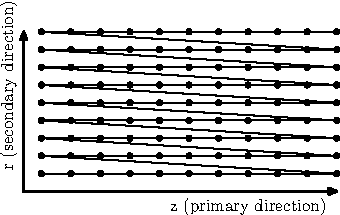
\includegraphics[origin=bl,height=40mm,angle=0]{./figures/Fieldmaps/order-1.pdf}
    \caption[Order of field values in a 2D field map in XZ orientation]{2D field map with primary direction corresponding to the longitudinal, secondary direction to the transverse direction}
    \label{fig:order1}
  \end{center}
\end{figure}

\begin{figure}[ht]
  \begin{center}
    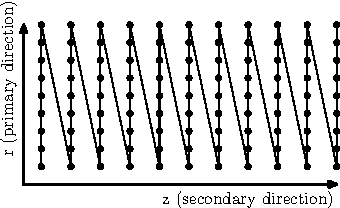
\includegraphics[origin=bl,height=40mm,angle=0]{./figures/Fieldmaps/order-2.pdf}
    \caption[Order of field values in a 2D field map in ZX orientation]{2D field map with primary direction corresponding to the transverse, secondary direction to the longitudinal direction}
    \label{fig:order2}
  \end{center}
\end{figure}

For the 2D dynamic case in XZ orientation there are four columns: $E_z$, $E_r$, an unused column and $H_t$ in this order. In the other orientation the first and the second column and the third and fourth column are interchanged.

On the second line of the header of a 1D, 2D or 3D T7 type of field map the beginning and the end of the electromagnetic field relative to the physical element in primary direction is written (in centimeters!). Also written on the second line is the number of {\bf mesh spacings}, corresponding to the {\bf number of grid points minus 1}. For the ASTRA compatible field maps this line is omitted.

On the third line is the frequency. For static cases this line is omitted. The frequency is on the second line of a AstraDynamic field map.

The fourth line corresponds to the second line but in secondary direction and the fifth accordingly for the tertiary direction. In the case of a 1D or 2D the fifth line is omitted since there is no tertiary direction. Those two lines are omitted in the ASTRA compatible field maps.

On the sixth line follows the first line with field values as described above.

Even though there is no secondary direction in the 1D case the header of a 1D field map is equal to its 2D equivalent: the elements can be provided with a boolean attribute FAST which has only an effect in conjunction with a 1D field map. The code then generates internally a 2D field map and the field strengths are interpolated as in the case of 2D and 3D field maps instead of being calculated using the Fourier coefficients. The fourth line determines the transverse dimension and the grain size of the produced mesh.

\noindent For examples of field maps see appendix~\ref{chp:app_fieldmaps} on page~\pageref{chp:app_fieldmaps} ff.

The field maps {\bf 1DProfile1} and {\bf 1DProfile2} are different from the rest since no actual fields are stored but a profile. They are used to represent the fringe fields of various elements. The fields have to be calculated using Enge functions \cite{enge} The fields calculated from this kind of field map depends on the kind of element in which they are used. Type 1 stores the coefficients of the Enge function whereas the type 2 stores the profile itself. From this profile the coefficients are calculated by solving a least-square equation. 

On the first line after the string describing the type of field map two integer numbers and a floating point number follow. The first integer number describes the number of Enge coefficients to be used for the entry fringe field, the second the equivalent for the exit fringe field. The floating point number specifies the gap height. On the second line the first value describes the beginning of the entry fringe field (in local coordinates; corresponds to {\sl zbegin\_entry} in Figure~\ref{fig:fringefields}), the second the origin of the Enge polynomial, the third the end of the fring field ({\sl zend\_entry}). The last number of this line is only used in Profile2 and specifies the number of grid points minus 1. The third line looks identically but the last value on this line is not used yet. The values on this line correspond to {\sl zbegin\_exit, origin of Enge function} and {\sl zend\_exit} in Figure~\ref{fig:fringefields}. The following lines are the coefficients of the Enge function in the case of 1DProfile1 and the profile in 1DProfile2, see appendix~\ref{chp:app_fieldmaps}.

\begin{figure}[ht]
  \begin{center}
    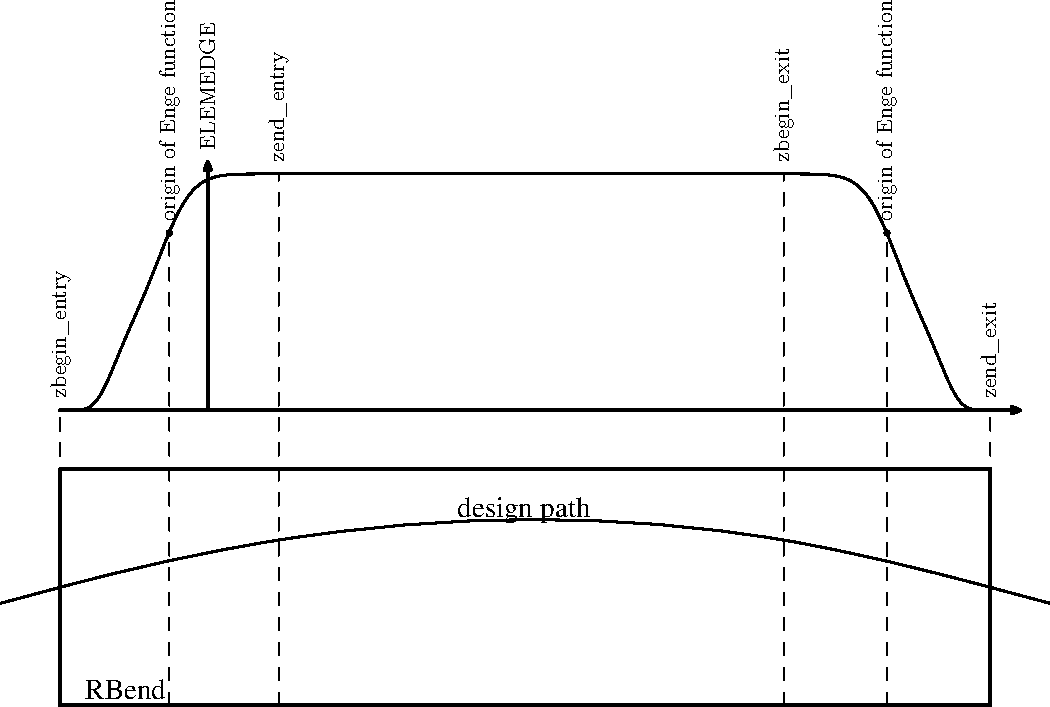
\includegraphics[origin=bl,height=100mm,angle=0]{./figures/Fieldmaps/profile-1.pdf}
    \caption{The profile of a rectangular bend and its corresponding design path.}
    \label{fig:fringefields}
  \end{center}
\end{figure}

\leftpointright As a general warning: be wise when you choose the type of field map to be used! The following three pictures show the longitudinal phase space after three gun simulations using different types of field maps. In the first picture, Figure~\ref{figure_1ddynamic_step82}, we used a 1D field map which stores a sampling of the electric field in longitudinal direction, $E_z$. From these values $E_z$, $E_r$ and $B_t$ off-axis are calculated resulting in a smooth field. All field maps we used are made of the same solution file from a Poisson/Superfish simulation.
\begin{figure}
  %
  \begin{center}
  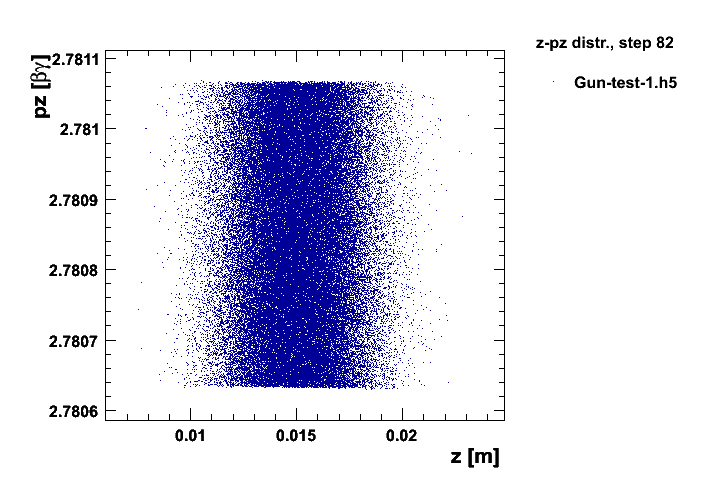
\includegraphics[origin=bl,height=80mm,angle=0]{./figures/Fieldmaps/1DDynamic_step82.png}
  %
  \caption{\label{figure_1ddynamic_step82}
    The longitudinal phase space after a gun simulation using a 1D field map (on-axis field) of the gun.
  }
  %
  \end{center}
%
\end{figure}

In Figure~\ref{figure_1ddynamic_fast_step82} we used the same on-axis field map as in the first but we used the FAST switch which constructs a 2D field map from the on-axis field maps. Between the grid points the fields are calculated using a linear interpolation. Here we see a structure which can be influence using more grid points in transverse direction.
\begin{figure}
  %
  \begin{center}
  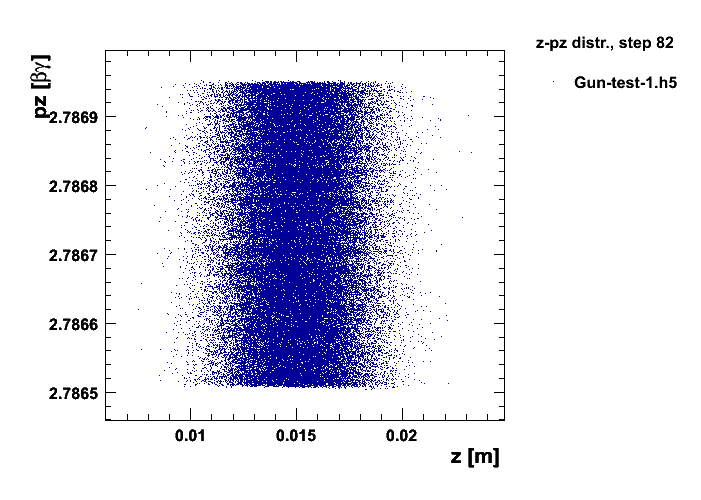
\includegraphics[origin=bl,height=80mm,angle=0]{./figures/Fieldmaps/1DDynamic_fast_step82.png}
  %
  \caption{\label{figure_1ddynamic_fast_step82}
    The longitudinal phase space after a gun simulation using a 1D field map (on-axis field) of the gun in combination with the FAST switch.
  }
  %
  \end{center}
%
\end{figure}
In the last picture, Figure~\ref{figure_2ddynamic_step82}, we generated directely a 2D field map from the solution file of Poisson/Superfish. Here we could observe two different structures: first the fine structure stemming from the linear interpolation and secondly a much stronger structure of unknow origin.
\begin{figure}
  %
  \begin{center}
  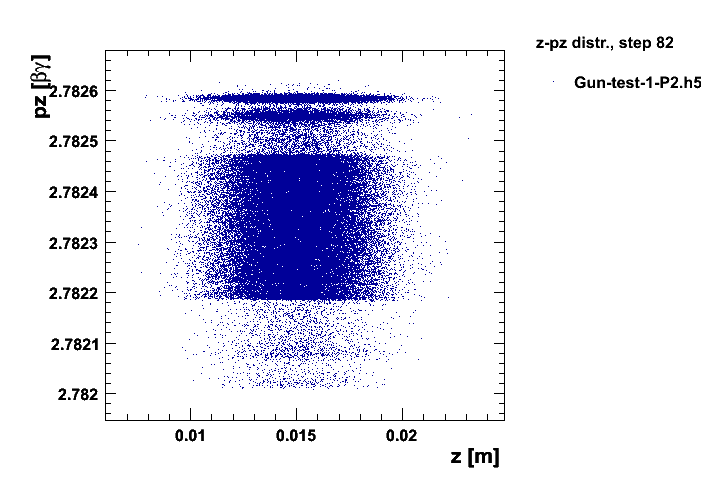
\includegraphics[origin=bl,height=80mm,angle=0]{./figures/Fieldmaps/2DDynamic_step82.png}
  %
  \caption{\label{figure_2ddynamic_step82}
    The longitudinal phase space after a gun simulation using a 2D field map of the gun generated by Poisson/Superfish.
  }
  %
  \end{center}
%
\end{figure}


\subsection{Field Maps from the Femaxx 3D Eigenmode Solver}

Electromagnetic field maps for beam dynamics calculations originate from a number of different
electromagnetic solvers, e.g. Superfish and similar codes.
%%
%%
Here, we describe the current status of work in progress which will, eventually,
allow the usage of field maps that have been computed with the femaxx $3$-dimensional
electromagnetic eigenmodal solver \cite{bib:arbenzetal2001,bib:arbenzetal2006}.
%%
%%
The femaxx code computes electromagnetic eigenmodes of resonant cavities of
arbitrary $3$-dimensional shape and boundary conditions.
%%
Unlike Superfish and similar $2$-dimensional codes, femaxx is not restricted in the
kind of geometry it can model. It is therefore possible to consider arbitrary
shapes and their inclusion in beam dynamics and particle tracking calculations.
%%
%%
Given a mesh of a $3$-dimensional geometry femaxx computes eigenomdal field
decompositions.
%%
The user then specifies sampling locations for the electromagnetic eigenfields.
%%
At present, sampling locations are specified in terms of a cylinder shape,
i.e. the user indicates the cylinder axis, the radial cylinder vector and 
the number of sampling locations in axial, radial and azimuthal directions.
%%
Once the eigenmodal solution has been computed the fields are sampled at
these locations and stored in the T7 file format, for subsequent use in \opal.
%%
Considerable effort has been spent for the validation and benchmarking of
beam dynamics calculations based on T7 field maps computed with femaxx.
%%
A pillbox cavity, i.e. a cylinder shape with a radius $r = 4.7$cm and
height $h = 3$ cm, has been chosen for benchmarking purposes,
due to the availability of an analytical solution.
%%
The analytical resonance frequency of the dominant mode is $2.441$ GHz.
%%
%%
We have compared two cases with \opal: (1) The analytical solution has been
sampled within a cylinder volume, stored into a T7 file and used in an \opal\
run; (2) the same pillbox shaped geometry has been discretization into tetrahedra
and the eigenmodal fields were calculated with femaxx.
%%
These two cases were then compared, resulting in the following conclusions:
%%
(1) Using a relatively coarse mesh with some $110'000$ tetrahedra, the difference
between the analytical and the numerical solution was usually smaller than
$1$ percent.
%%
(2) Using an adaptively refined mesh, the difference between analytical and
numerical solutions decreased below $1$ pro mille. The mesh is shown
in the figure (\ref{figure_pillbox_adaptively_refined_mesh}).
%%
(3) It is thereofore imperative to usa a tetrahedral mesh which has been
refined around the beam axis. It is definitely more efficient to use local
refinement, based on physical argument, than simply refine the complete
mesh in a uniform manner.
%%


We are now working towards benchmarking more complicated shapes in order to
assess requirements w.r.t to meshes and modeling geometry so that we
achieve the same or better accuracy as has been obtained from field
maps that were computed with Superfish like solvers based on azimuthal symmetry.

\begin{figure}
  %
  \begin{center}
  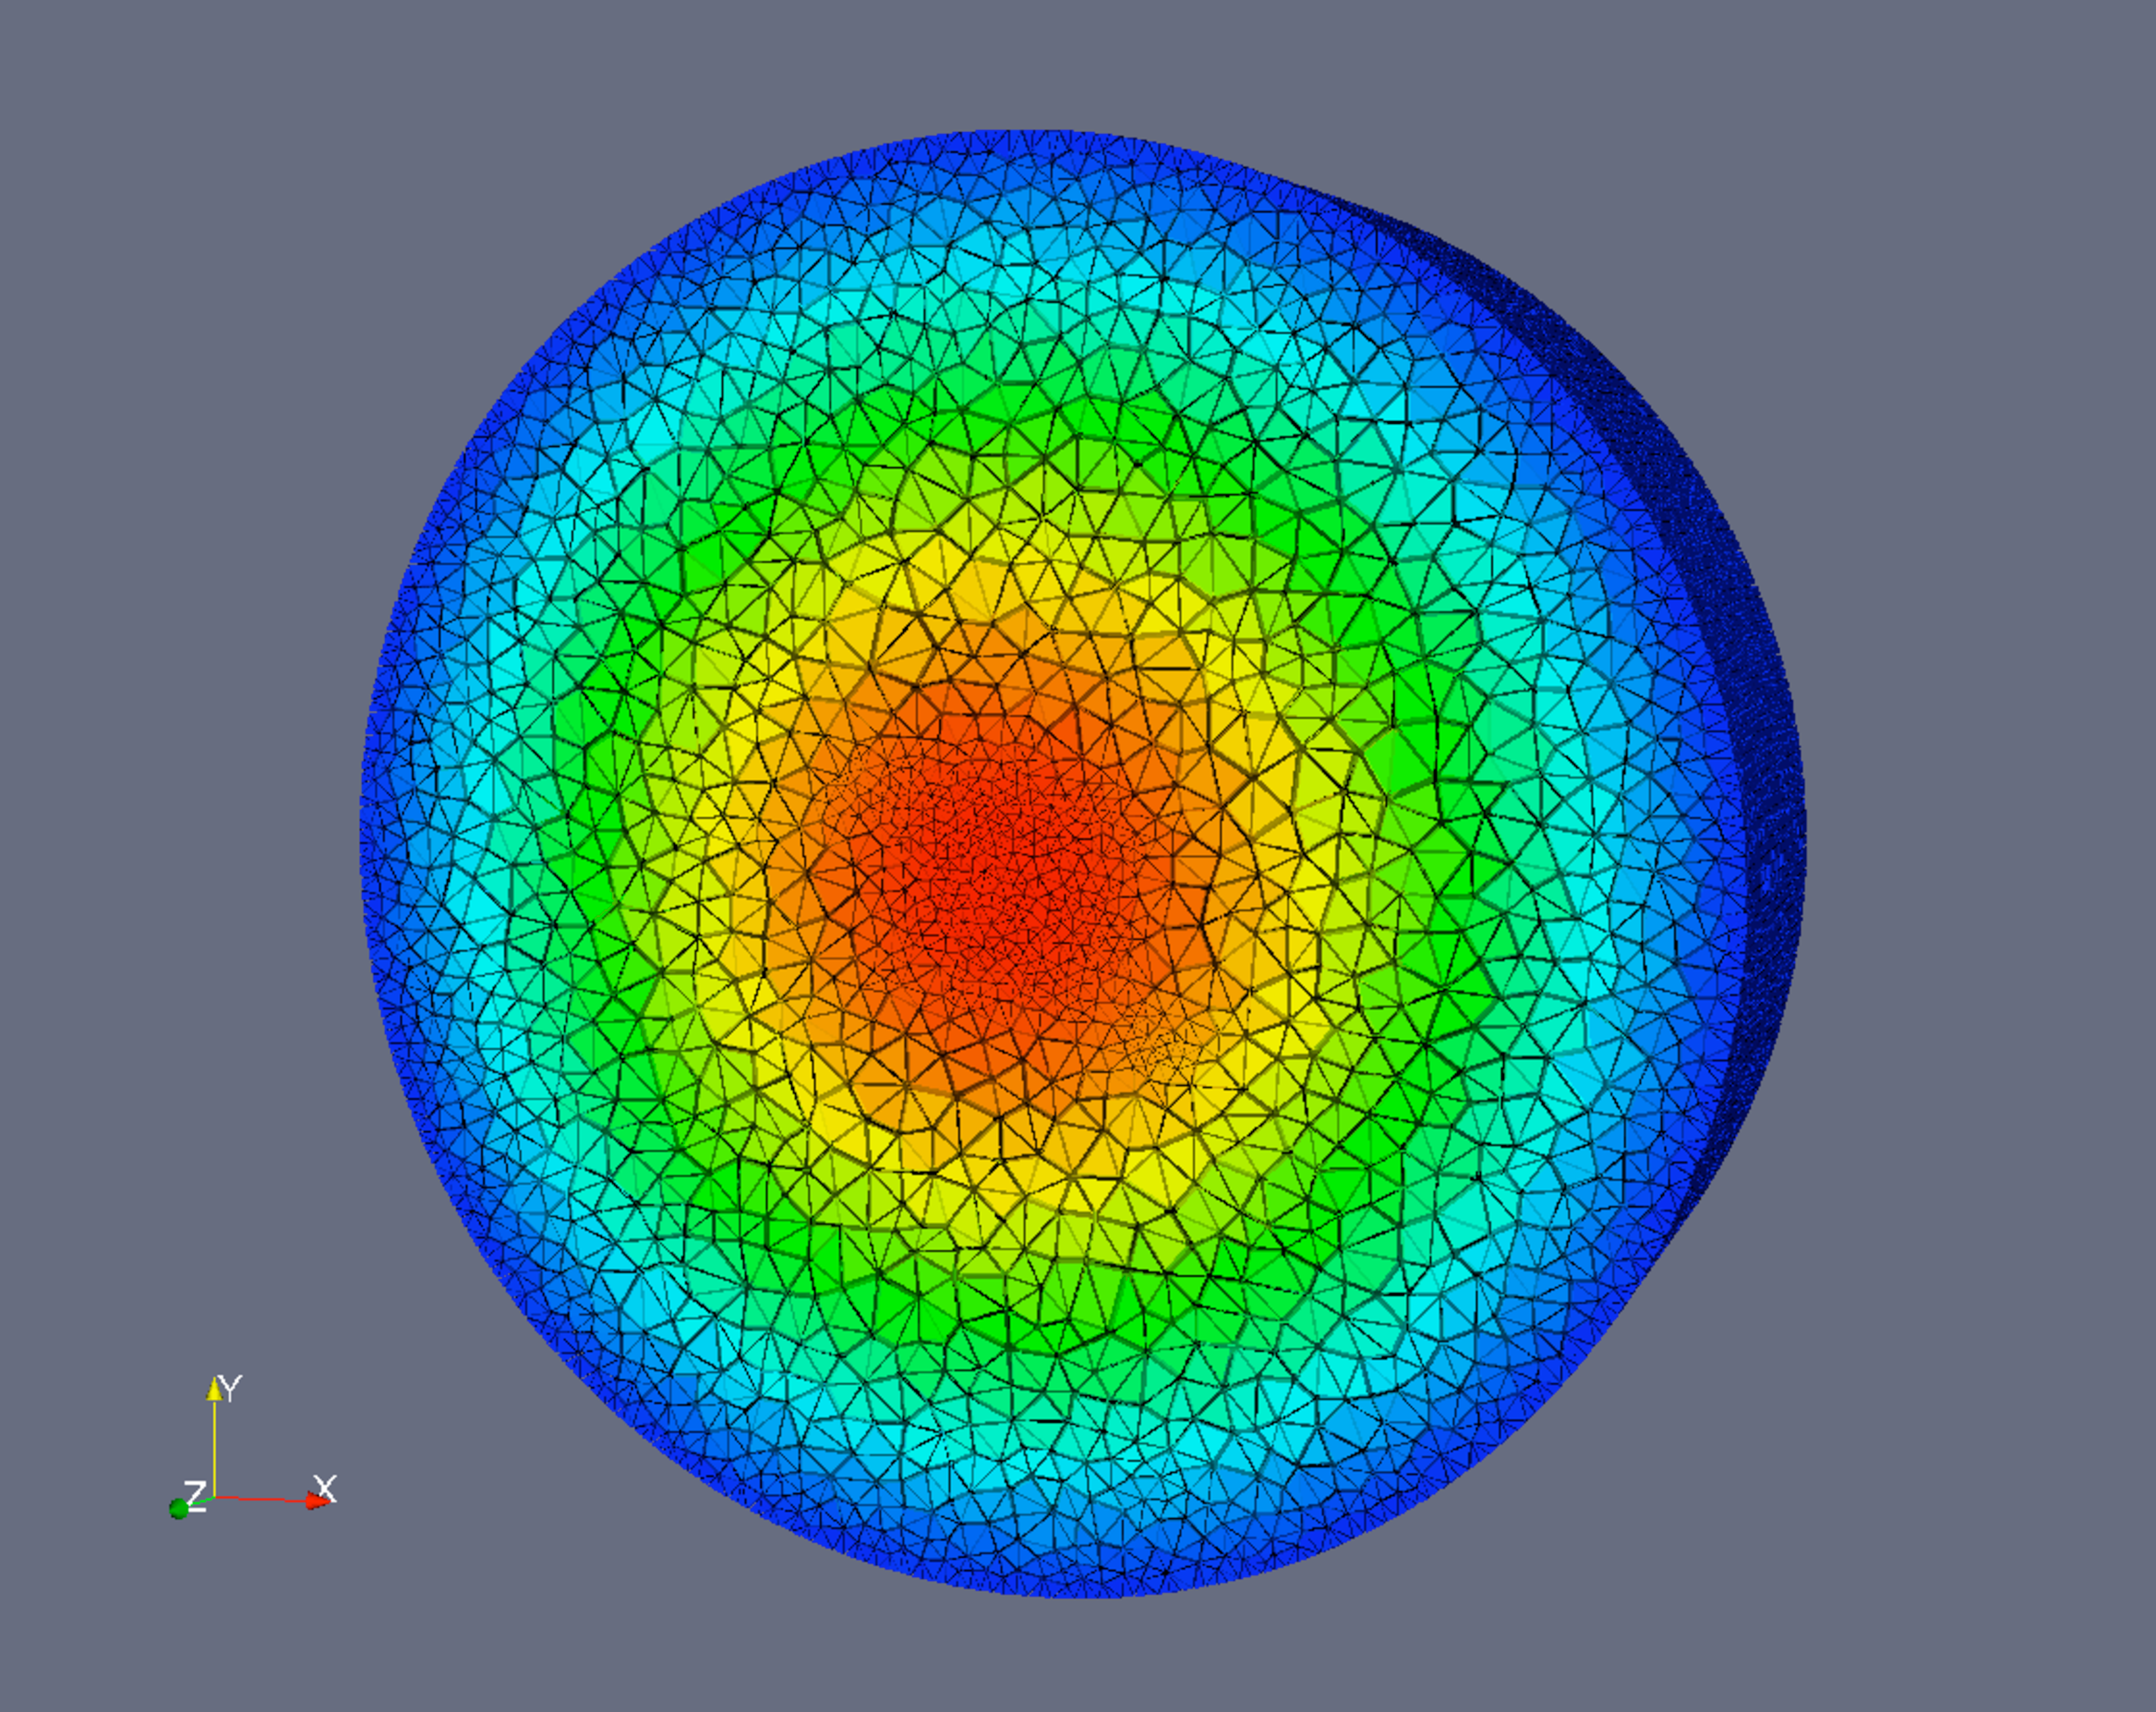
\includegraphics[origin=bl,width=80mm,angle=0]{./figures/adaptivePillboxMesh.pdf}
  %
  \caption[Tetrahedral mesh of a pillbox shaped cavity]{\label{figure_pillbox_adaptively_refined_mesh}
    We show the discretization of a pillbox shaped cavity geometry
        into a tetrahedral mesh. The mesh has been adaptively
        refined so that the region around the cylinder axis is
        decomposed into smaller tetrahedra than those which are
        further away from the axis.
  }
  %
  \end{center}
%
\end{figure}

\clearpage
\subsection{Output}
The data is stored in the H5Part file-format (\url{http://h5part.web.psi.ch/}) and can be analysed
using the H5PartRoot (\url{http://amas.web.psi.ch/tools/H5PartROOT/index.html}). The frequency 
of the data output (phase space and some statistical quantities) can be set using the \secref{\texttt{OPTION} statement}{option}, 
statement and the flag PSDUMPFREQ. The file is named like in input file but the extension is {\tt .h5}. 

\begin{figure}[ht]
 \begin{center}
 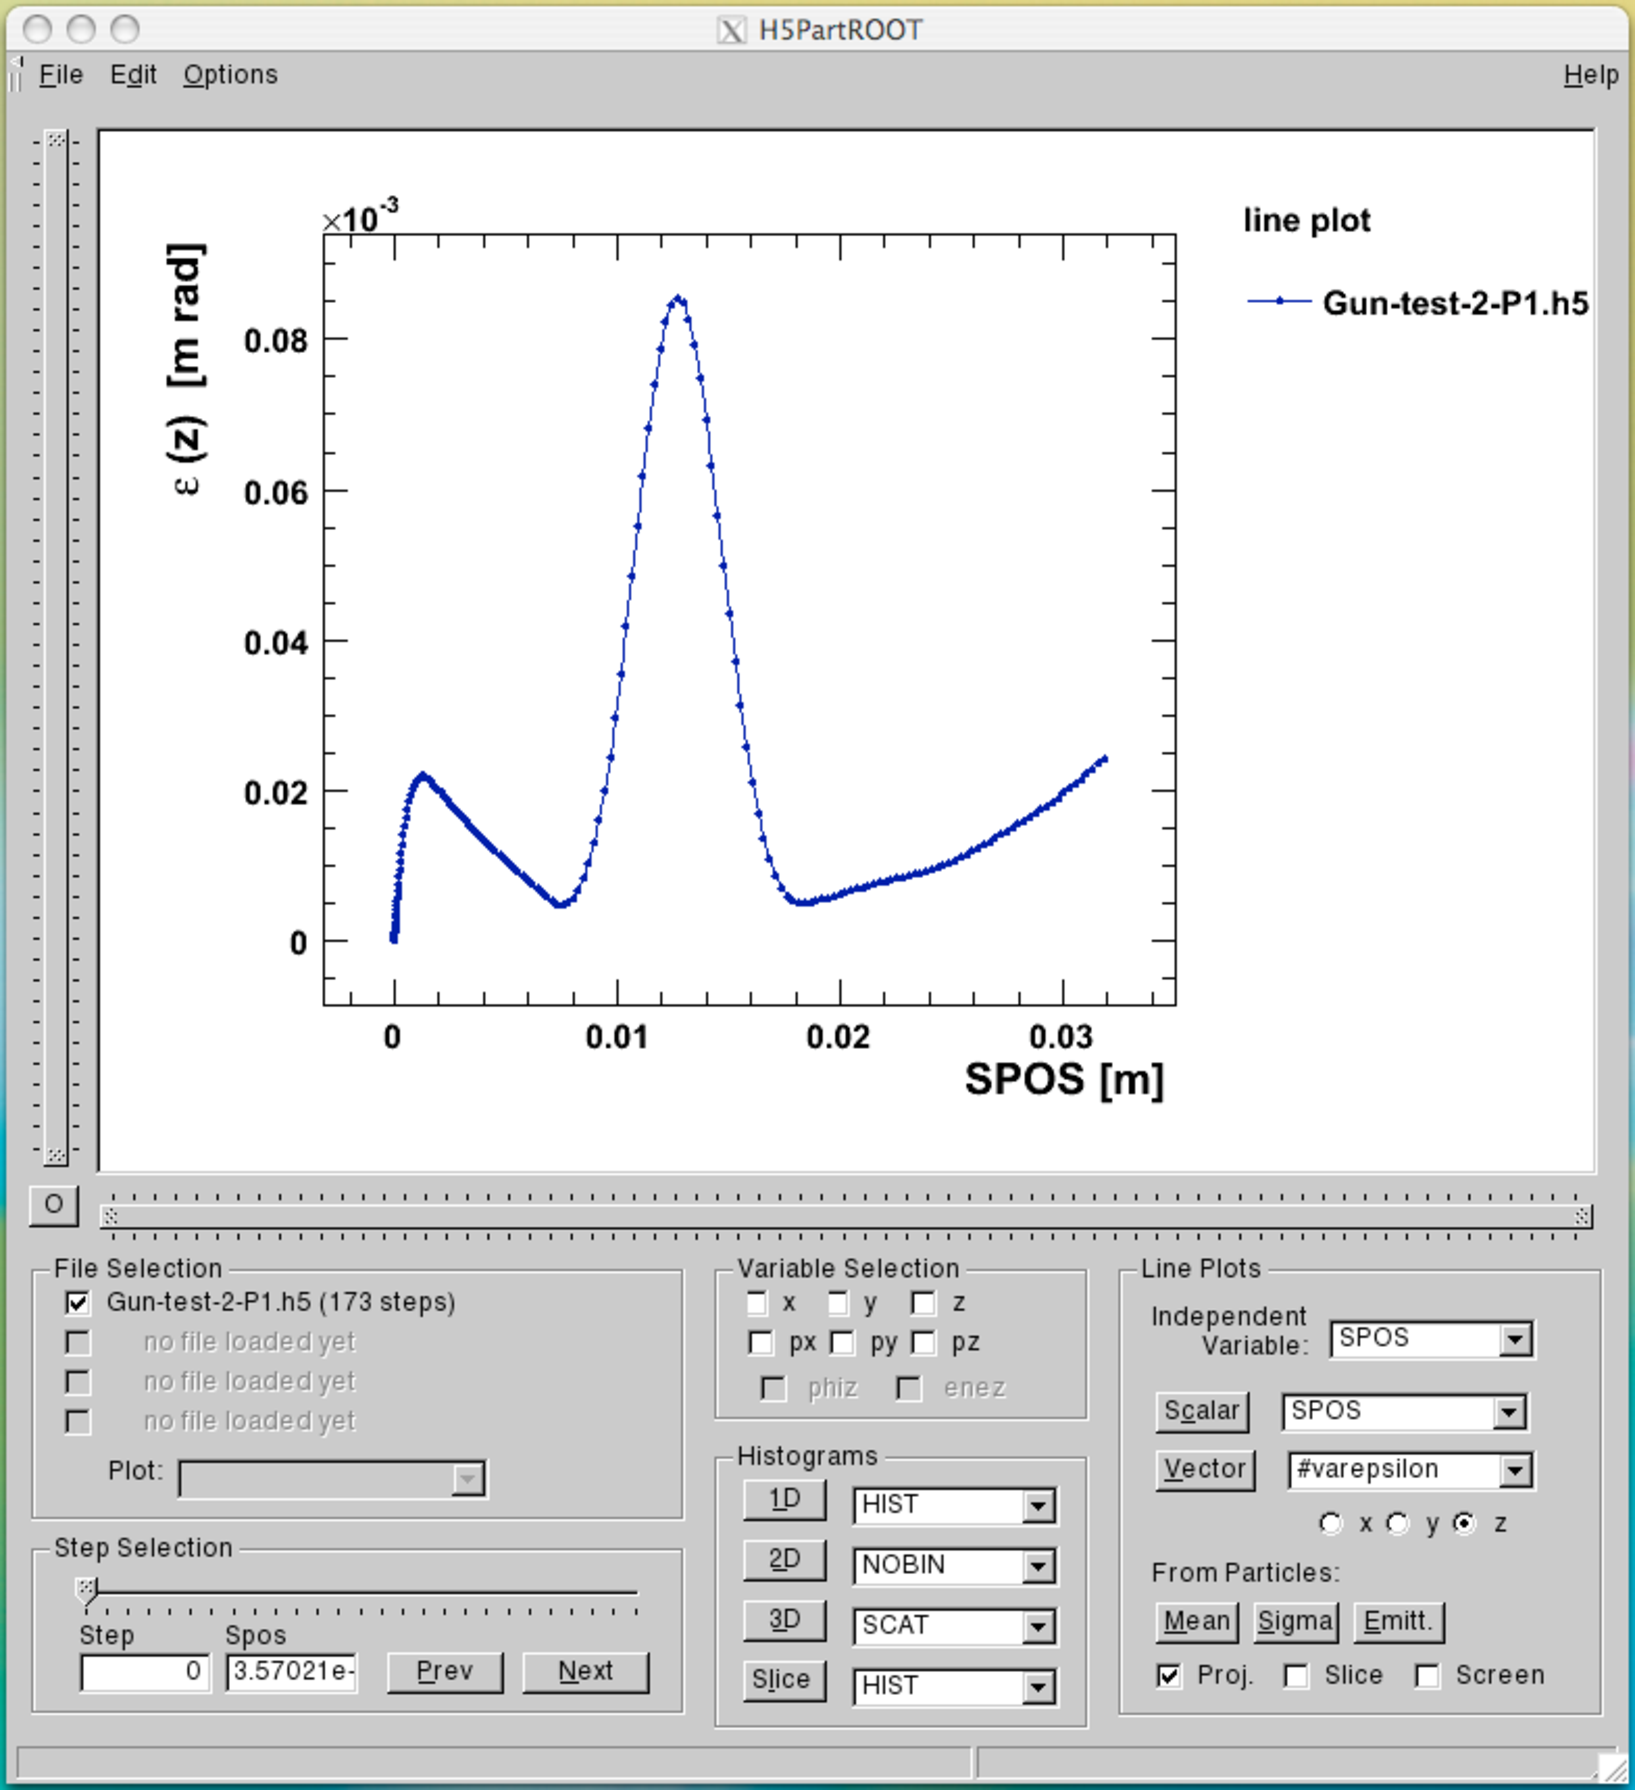
\includegraphics[width=0.45\linewidth,angle=0]{figures/H5rootPicture1}
  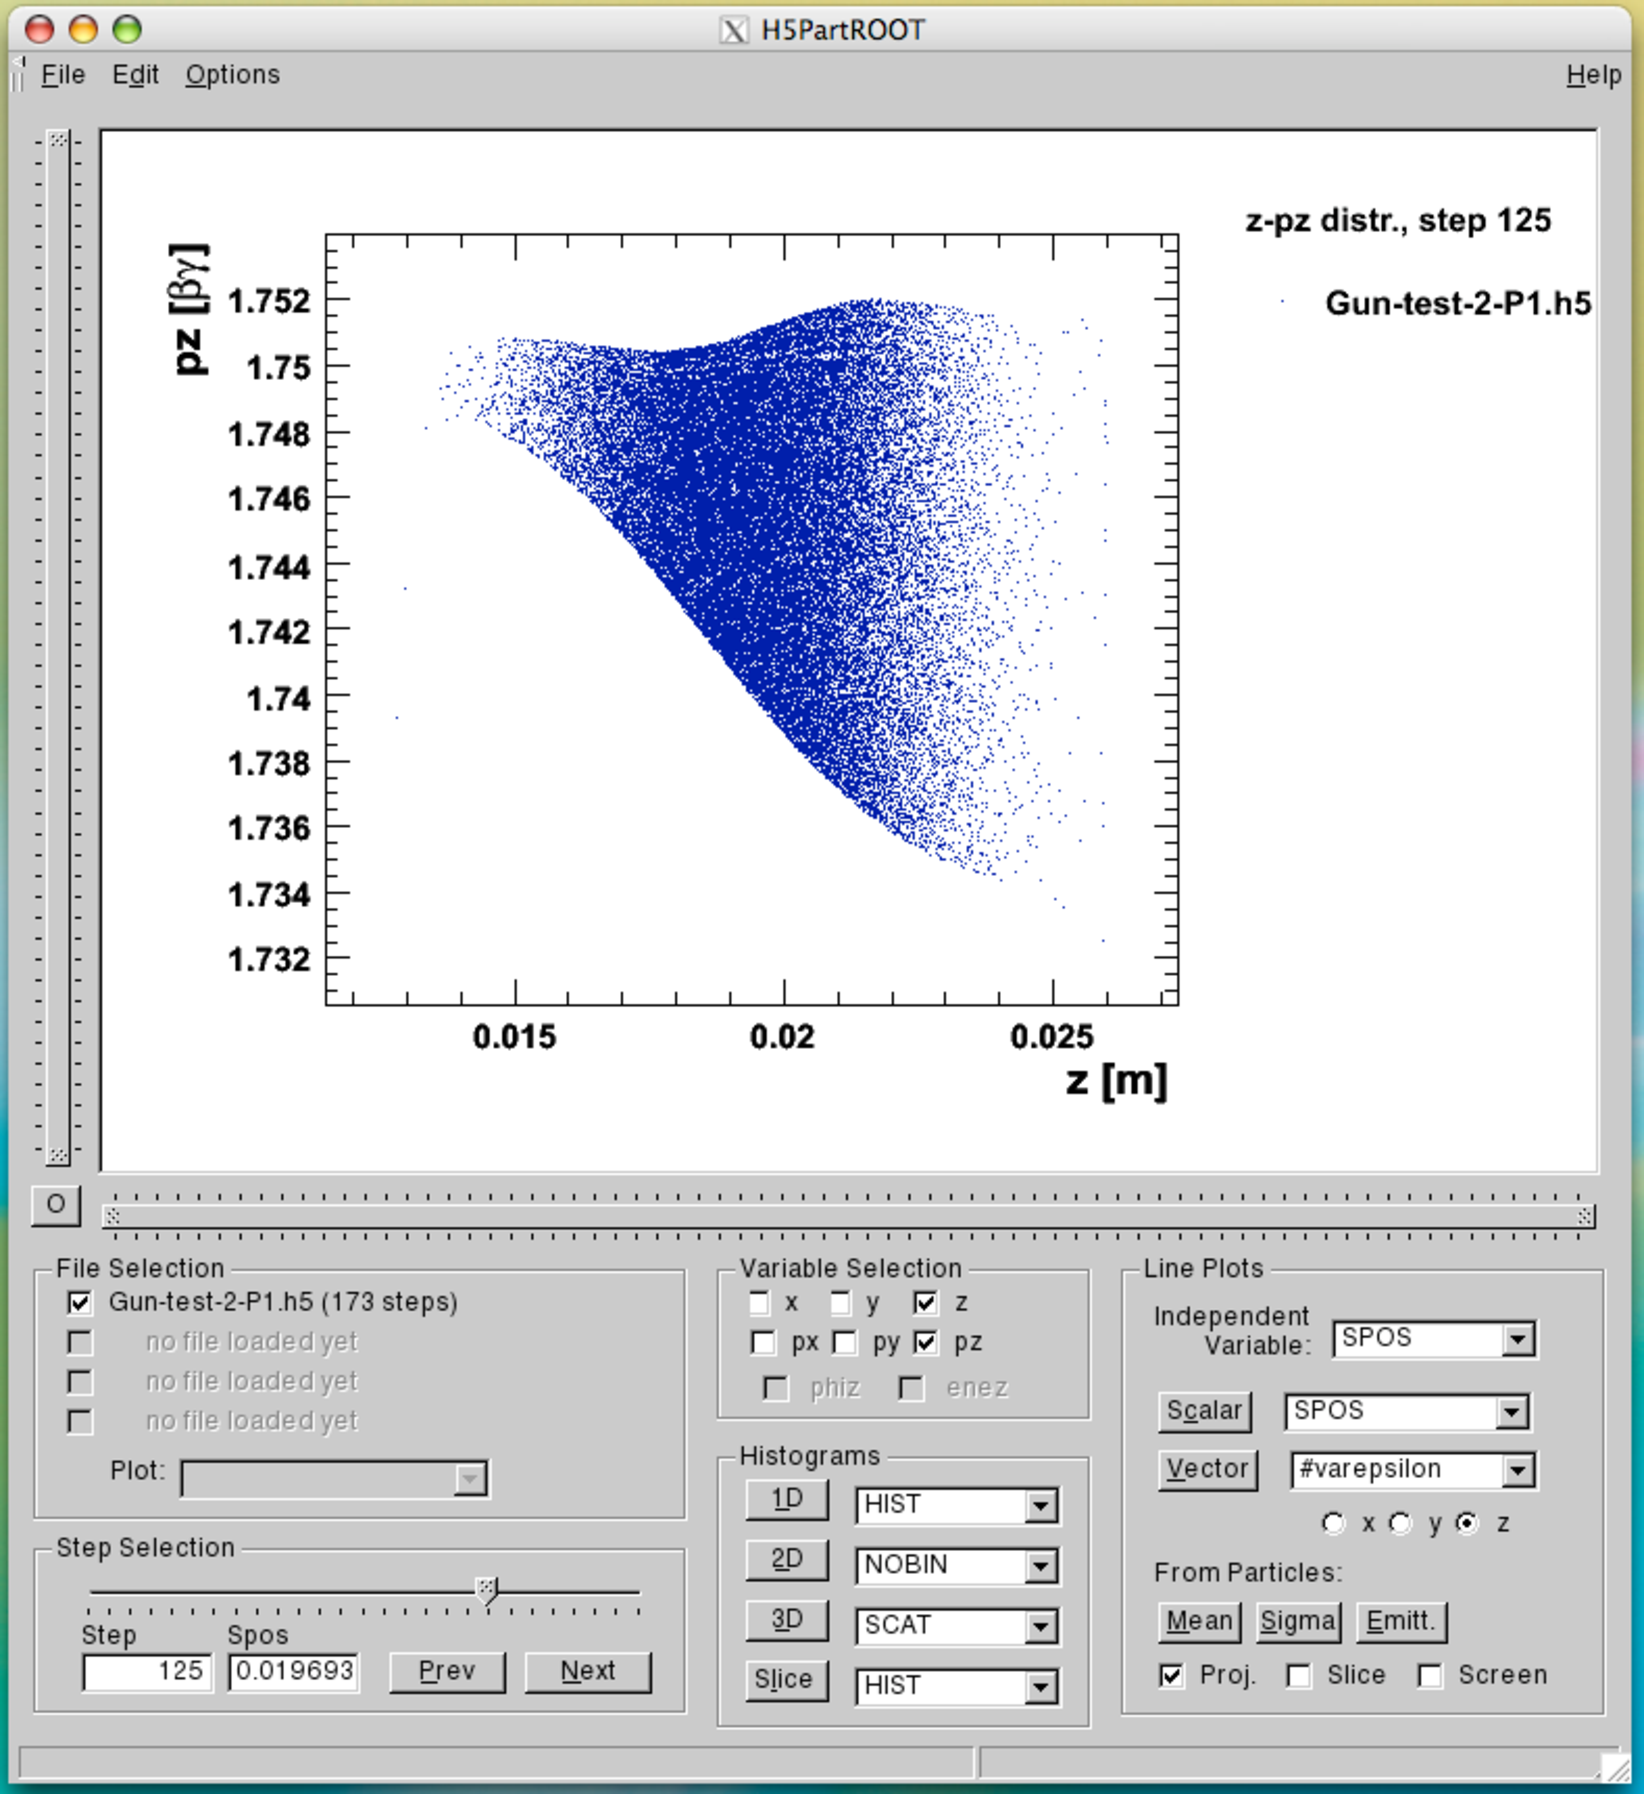
\includegraphics[width=0.45\linewidth,angle=0]{figures/H5rootPicture2}
  \caption{H5PartROOT enables a variety of data analysis and post processing task on \opal\ data}
  \label{fig:h5root1}
 \end{center}
\end{figure}



\begin{figure}[ht]
 \begin{center}
   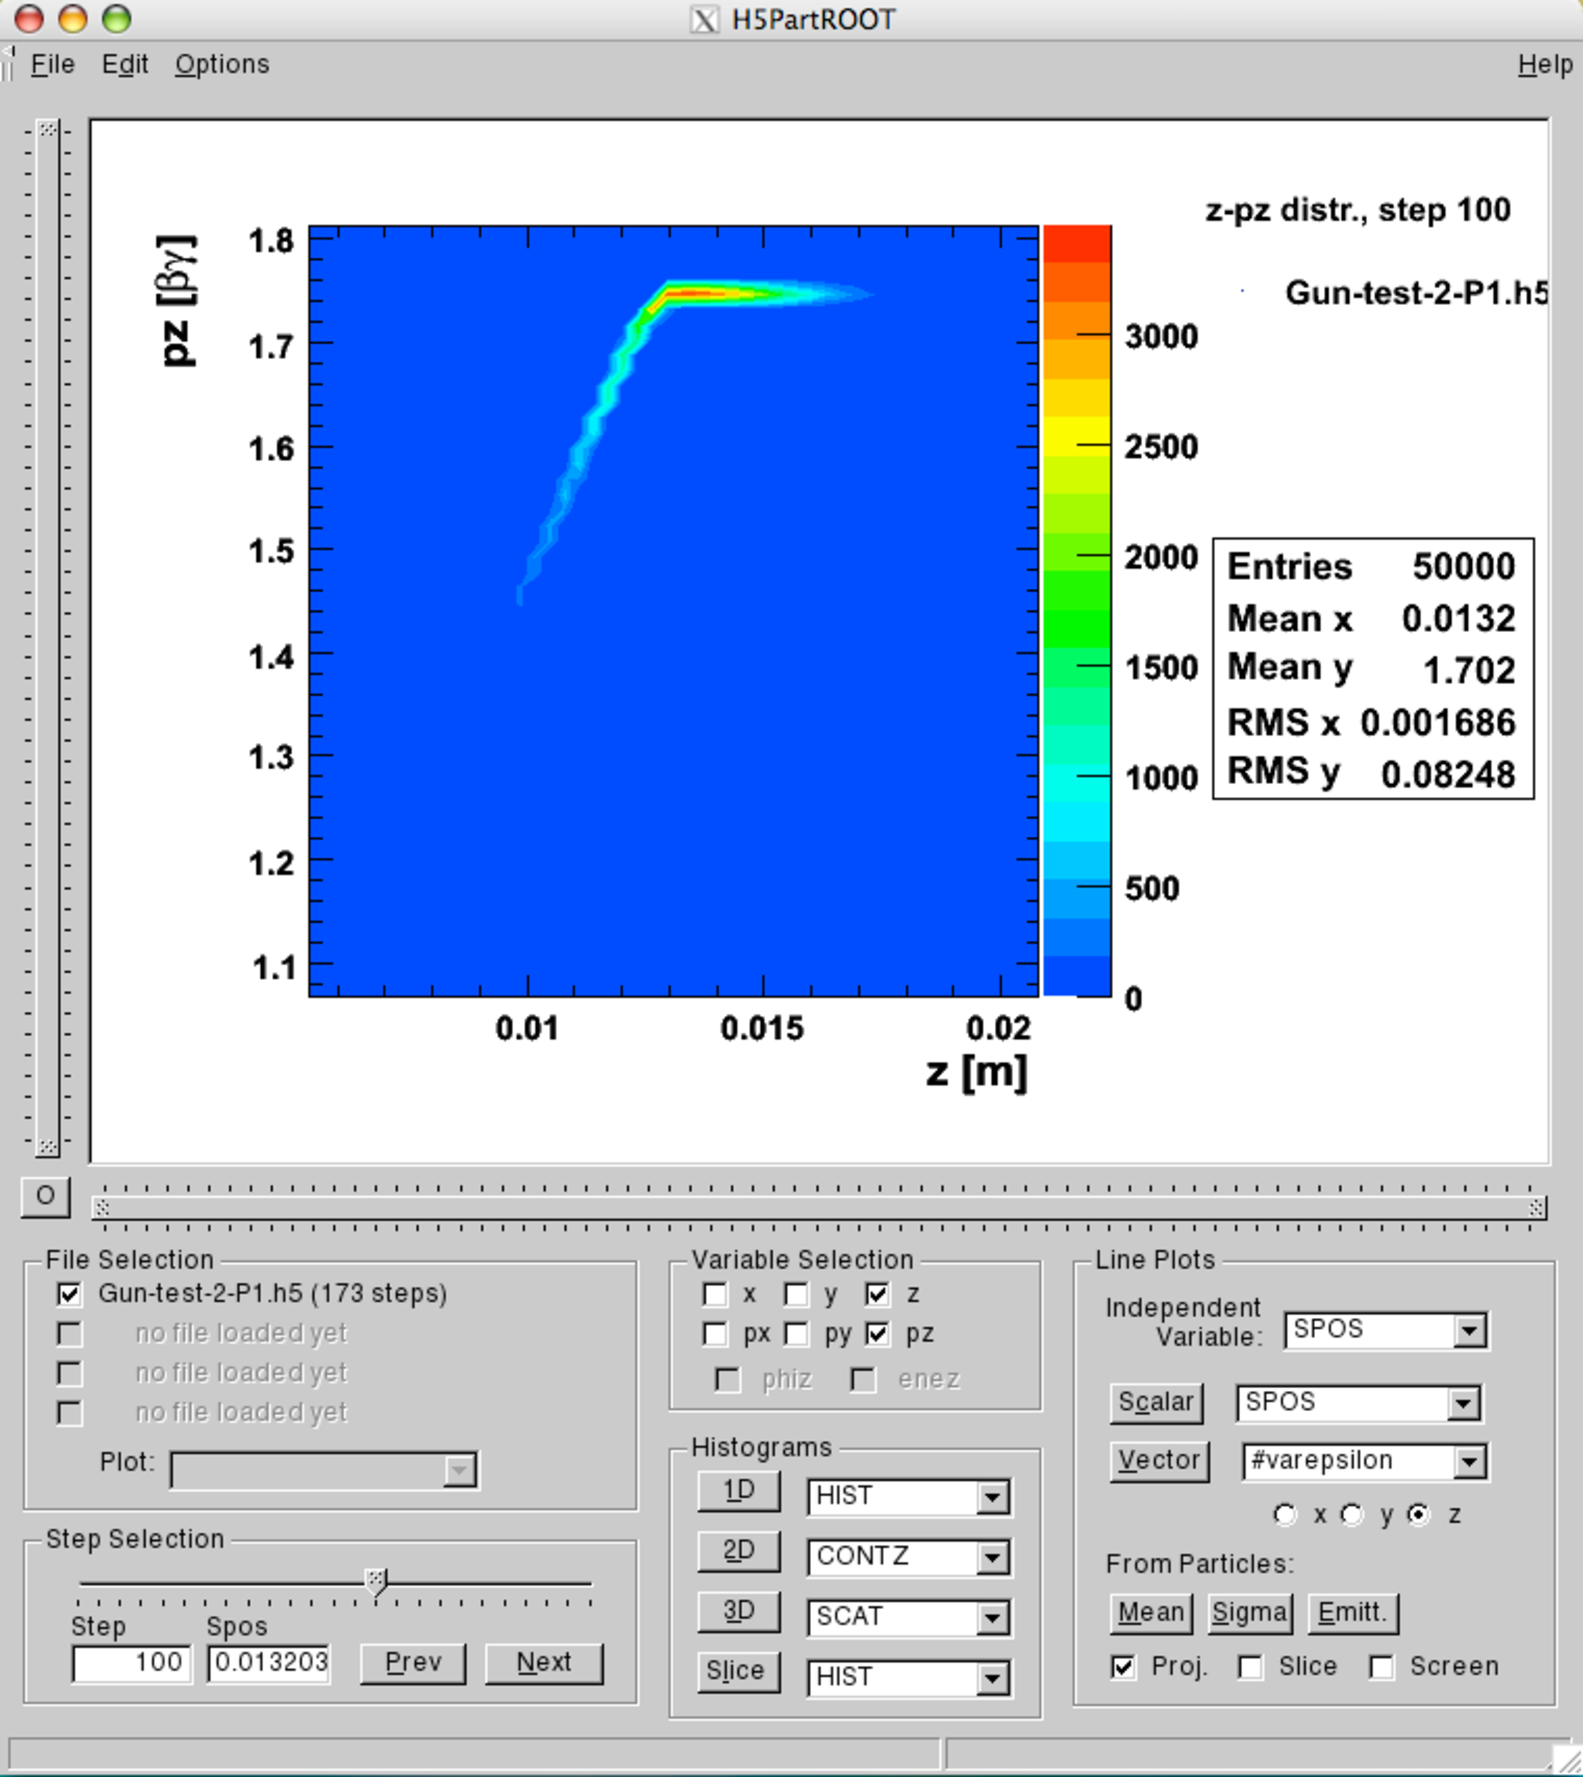
\includegraphics[width=.9\linewidth,angle=0]{figures/H5rootPicture3}
  \caption{Example of a longitudinal phase space shown with H5PartROOT}
  \label{fig:h5root2}
 \end{center}
\end{figure}



An ASCII file with statistical beam 
parameters is stored in a {\tt .stat} file. An SDDS file output is in preparation.

\section{\opalcycl}
\label{sec:opalcycl}
\index{opalFlavours}

\subsection{Introduction}

\opalcycl\ is a fully three-dimensional parallel beam dynamics simulation program dedicated to future high intensity cyclotrons 
which is capable of doing single particle tracking for conventional orbit designs on single computation node and 
multiple particles tracking in a parallel environment which takes into account both space charge effects 
 
For the first time in the cyclotron community, \opalcycl\ has the capability to track multiple bunches simultaneously
and take into account the beam-beam effects of the radial neighboring bunches (we call it neighboring bunch effects for short)
by using a self-consistent numerical simulation model.

According to the number of particles defined (by the argument \texttt{NPART} in \texttt{BEAM}, see Section \ref{sec:beam}) , 
\opalcycl\ selects the following three operation modes automatically:

\begin{description}

\item[Single Particle Tracking mode]

  In this mode, only one particle is tracked, either with acceleration or not.  Working in this mode, \opalcycl\
  can be used as a tool during the preliminary design phase of a cyclotron.  

  The 6D parameters of a single particle in the initial local frame must be read from a file. To do this, in the \opal\ input file, 
  the command line \texttt{DISTRIBUTION}(See Chapter \ref{chp:distribution}) should be defined like this:
\begin{verbatim}
  Dist1: DISTRIBUTION, DISTRIBUTION=fromfile,
         FNAME="PartDatabase.dat";
\end{verbatim}
 where the file $PartDatabase.dat$ should have two lines:
\begin{verbatim}
 1
 0.001 0.001   0.001   0.001   0.001  0.001    
\end{verbatim}
The number in the first line is the total number of particles.
In the second line the data represents $x, p_x, y,$$ p_y, z, p_z$ with the reference particle 
in the local frame. The units are described in section \ref{sec:variablesopalcycl}.

Please don't try to run his mode in parallel environment. You should believe that a single processor of the 21st century is capable of doing
the single particle tracking.  

\item[Tune Calculation mode]

  In this mode, two particles are tracked, one with all data is set to zero is the reference particle and another one is an off-centering particle 
  which has a little shift from the other one in both $r$ and $z$ directions. Working in this mode, \opalcycl\ can 
  calculate the betatron oscillation frequency $\nu_r$ and $\nu_z$ for different energies to evaluate the focusing characteristics 
  for a given magnetic field.

  Like the single particle tracking mode, 
  the 6D parameters of the two particles in initial local frame must be read from a file, too.
  In the file should has three lines:
\begin{verbatim}
 2
 0.0   0.0   0.0   0.0   0.0   0.0  
 0.001 0.0   0.0   0.0   0.001  0.0    
\end{verbatim}

When the total particle number equals 2, this mode is triggered automatically.
Only the element \texttt{CYCLOTRON} in the beam line is used and other elements are omitted if any exists.

Please don't try to run his mode in parallel environment, either.


\item[Multi-bunches tracking mode]

  In this mode, large scale particles can be tracked simultaneously, either with space charge or not, 
  either single bunch or multi-bunches, either serial or parallel environment, 
  either reading the initial distribution from a file or generating a typical distribution,  
  either running from the beginning or restarting from the last step of a former simulation.

  Because this is the main mode as well as the key part of \opalcycl, 
  we will describe this in detail in Section \ref{sec:opalcycl:MultiBunch}.

\end{description}  
  
Generally speaking, the following aspects may be considered for quantitatively studying high intensity beam dynamics in cyclotrons:
  \begin{itemize}
  \item large scale particles, as many as possible, which is of course limited by computer sources;
  \item measured magnetic field map or numerical calculated field with high precision;
  \item numerical integrator with high precision;
  \item powerful parallel Poisson solver with high precision and resolution;
  \item imperfection and misalignment of the machine;
  \item the influences of other factors induced by high intensity, such as beam-beam effects and weak field effects induced in the cavities. 
  \end{itemize}
  In the following sections of this chapter, some of the above issues will be described in detail for \opalcycl.

\subsection{Field Map}
\label{sec:opalcycl:fildmap}
In \opalcycl, the magnetic field is read from an ASCII type file. The field data should be stored in the cylinder coordinates frame
( because the field map on the median plane of the cyclotron is usually measured in this frame ). 

There are two possible situations. One is the real field map on median plane of the exist cyclotron machine using measurement equipment.
Limited by the narrow gaps of magnets, in most cases with cyclotrons, only vertical field $B_z$ on the median plane ($z=0$) is measured.
Since the magnetic field data off the median plane field components is necessary for those particles with $z \neq 0$, the field need to be expanded in $Z$ direction. 
According to the approach given by Gordon and Taivassalo, by using a magnetic potential and measured $B_z$ on the median plane, 
at the point $(r,\theta, z)$ in cylindrical polar coordinates, the 3$th$ order field can be written as    
\begin{eqnarray}\label{eq:Bfield}
  B_r(r,\theta, z) & = & z\frac{\partial B_z}{\partial r}-\frac{1}{6}z^3 C_r, \nonumber\\    
  B_\theta(r,\theta, z) & = & \frac{z}{r}\frac{\partial B_z}{\partial \theta}-\frac{1}{6}\frac{z^3}{r} C_{\theta}, \\     
  B_z(r,\theta, z) & = & B_z-\frac{1}{2}z^2 C_z,  \nonumber    
\end{eqnarray}
where $B_z\equiv B_z(r, \theta, 0)$ and  
\begin{eqnarray}\label{eq:Bcoeff}
  C_r & = & \frac{\partial^3B_z}{\partial r^3} + \frac{1}{r}\frac{\partial^2 B_z}{\partial r^2} - \frac{1}{r^2}\frac{\partial B_z}{\partial r} 
        + \frac{1}{r^2}\frac{\partial^3 B_z}{\partial r \partial \theta^2} - 2\frac{1}{r^3}\frac{\partial^2 B_z}{\partial \theta^2}, \nonumber  \\    
  C_{\theta} & = & \frac{1}{r}\frac{\partial^2 B_z}{\partial r \partial \theta} + \frac{\partial^3 B_z}{\partial r^2 \partial \theta}
        + \frac{1}{r^2}\frac{\partial^3 B_z}{\partial \theta^3},  \\
  C_z & = & \frac{1}{r}\frac{\partial B_z}{\partial r} + \frac{\partial^2 B_z}{\partial r^2} + \frac{1}{r^2}\frac{\partial^2 B_z}{\partial \theta^2}. \nonumber
\end{eqnarray}

All the partial differential coefficients are on the median plane and can be calculated by interpolation. \opalcycl\ uses  Lagrange's  5-point formula.

The other situation is to calculate the field on the median plane or the 3D fields of the working gap for interesting region numerically by creating 3D model using commercial software,
such as TOSCA, ANSOFT and ANSYS during the design phase of a new machine. If the field on the median plane is calculated, the field off the median plane can be obtained using 
the same expansion approach as the measured field map as described above. However, the 3D fields of the entire working gap should be more accurate than 
the expansion approach  especially at the region not so close to the median plane in $Z$ direction.

In the current version, we implemented the three specific type field-read functions $Cyclotron::$$getFieldFromFile()$ of the median plane fields.
That which function is used is controlled by the parameters TYPE of CYCLOTRON (see Section \ref{sec:cyclotron}) in the input file.
\begin{enumerate}
\item TYPE=CARBONCYCL. 
Program reads in the median plane field date $B_z$ (in kGauss) from a file in which the data is arranged as shown in Fig.\ref{fig:CYCLField}.
This function is originally for the field map of the PSI 450 MeV C12 cyclotron which is under design but can serve as a simple way to import ASCII 
field maps.
\begin{figure}[ht]
  \begin{center}
    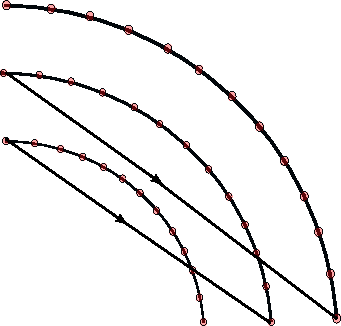
\includegraphics[origin=bl,height=40mm]{./figures/cyclotron/CarbonFieldFormat.pdf}
    \caption{2D field map on the median plane with primary direction corresponding to the azimuthal direction, secondary direction to the radial direction}
    \label{fig:CYCLField}
  \end{center}
\end{figure}
We need to add 6 parameters at the header of a plain $B_z$ (kGauss) data file, namely, 
$r_{min}$, $\Delta r$ (cm), $\theta_{min}$, $\Delta \theta$ (deg), 
$N_\theta$ (total data number in each arc path of azimuthal direction) and $N_r$ (total path number along radial direction). 
If $\Delta r$ or $\Delta \theta$ is decimal, one can set its negative opposite number. For instance, if $\Delta \theta = \frac{1}{3}^\circ$, the fourth line of the header should be set to -3.0. 
Example showing the above explained format: 
\begin{fmpage}
\begin{footnotesize}
\begin{verbatim}
3.0e+03
10.0
0.0
-3.0
300
161
1.414e-03  3.743e-03  8.517e-03  1.221e-02  2.296e-02 
3.884e-02  5.999e-02  8.580e-02  1.150e-01  1.461e-01 
1.779e-01  2.090e-01  2.392e-01  2.682e-01  2.964e-01 
3.245e-01  3.534e-01  3.843e-01  4.184e-01  4.573e-01 
                        ......
\end{verbatim}
\end{footnotesize}
\end{fmpage}
\item TYPE=CYCIAE. 

Program reads in the median plane fields $B_z$ calculated by ANSYS\,10.0.  This function is originally for the 100 MeV cyclotron of CIAE,
 whose isochronous fields is numerically computed by by ANSYS. The median plane fields data is output by reading the APDL (ANSYS Parametric Design Language) script
during the post-processing phase (you may need to do minor changes to adapt your own cyclotron model):
\begin{fmpage}
\begin{footnotesize}
\begin{verbatim}
/post1
resume,solu,db
csys,1
nsel,s,loc,x,0
nsel,r,loc,y,0
nsel,r,loc,z,0
PRNSOL,B,COMP

CSYS,1
rsys,1

*do,count,0,200
   path,cyc100_Ansys,2,5,45
   ppath,1,,0.01*count,0,,1
   ppath,2,,0.01*count/sqrt(2),0.01*count/sqrt(2),,1

   pdef,bz,b,z
   paget,data,table
   
   *if,count,eq,0,then
      /output,cyc100_ANSYS,dat
      *STATUS,data,,,5,5
      /output
   *else
      /output,cyc100_ANSYS,dat,,append
      *STATUS,data,,,5,5
      /output
   *endif
*enddo
finish
\end{verbatim}
\end{footnotesize}
\end{fmpage}
By run this in ANSYS, you can get a fields file with the name $cyc100_ANSYS.data$. 
You need to  put 6 parameters at the header of the file, namely, $r_{min}$, $\Delta r$, $\theta_{min}$, $\Delta \theta$, 
$N_\theta$(total data number in each arc path of azimuthal direction) and $N_r$(total path number along radial direction). 
If $\Delta r$ or $\Delta \theta$ is decimal,one can set its negative opposite number. This is useful is the decimal is unlimited. 
For instance,if $\Delta \theta = \frac{1}{3}^\circ$, the fourth line of the header should be -3.0. 
In a word, the fields are stored in the following format:
\begin{fmpage}
\begin{footnotesize}
\begin{verbatim}
0.0
10.0
0.0e+00
1.0e+00
90
201
 PARAMETER STATUS- DATA  ( 336 PARAMETERS DEFINED)
                  (INCLUDING    17 INTERNAL PARAMETERS)

      LOCATION                VALUE
        1       5       1   0.537657876    
        2       5       1   0.538079473    
        3       5       1   0.539086731    
                  ......
       44       5       1   0.760777286    
       45       5       1   0.760918663    
       46       5       1   0.760969074    

 PARAMETER STATUS- DATA  ( 336 PARAMETERS DEFINED)
                  (INCLUDING    17 INTERNAL PARAMETERS)

      LOCATION                VALUE
        1       5       1   0.704927299    
        2       5       1   0.705050993    
        3       5       1   0.705341275    
                  ......
\end{verbatim}
\end{footnotesize}
\end{fmpage}


\item If the value of TYPE is other string rather than above two, programme read in field data from the PSI format field file {\small{ZYKL9Z.NAR}}. 
We add 4 parameters at the header of the file, namely, $r_{min}$, $\Delta r$,
$\theta_{min}$ and $\Delta \theta$. This is the default function for reading fields data.
If $\Delta r$ or $\Delta \theta$ is decimal,one can set its negative opposite number. This is useful is the decimal is unlimited. 
For instance,if $\Delta \theta = \frac{1}{3}^\circ$, the fourth line of the header should be -3.0.  
\end{enumerate}
{\bfseries You should revise the function or write your own function according to the instructions in the code to match your own field
format if it is different to above three types.}  
The generic interface function for both the 2D measured map and the 3D field from file will be available in a later version.\\ 

For more detail about the parameters of CYCLOTRON, please refer to Section \ref{sec:cyclotron}.

In the current version of \opalcycl, the RF cavities are treated as straight lines with infinitely narrow gaps
and the electric field is a $\delta$ function plus a transit time correction.
the two-gap cavity is treated as two independent single-gap cavities. the spiral gap cavity is not implemented yet.

For more detail about the parameters of cyclotron cavities, see Section \ref{sec:cavity-cycl}.

The voltage profile of a cavity gap  is read from ASCII file. Here is an example:
\begin{verbatim}
6  
0.00      0.15      2.40 
0.20      0.65      2.41 
0.40      0.98      0.66 
0.60      0.88     -1.59 
0.80      0.43     -2.65 
1.00     -0.05     -1.71 
\end{verbatim}
The number in the first line means 6 sample points and in the following lines the three values represent the normalized distance to 
the inner edge of the cavity, the normalized voltage and its derivative respectively.

\subsection{Particle Tracking and Accelerating}  

The precision of the tracking methods is vital for the entire simulation process, especially for long distance tracking jobs.
\opalcycl\ uses a 4th order Runge-Kutta algorithm and the second order Leap-Frog scheme. The 4th order Runge-Kutta algorithm needs 4 the external magnetic field evaluation in each time step $\tau$ .
During the field interpolation process, for an arbitrary given point the code first interpolates Formula $B_z$
for its counterpart on the median plane and then expands to this give point using (\ref{eq:Bfield}). 

After each time step $i$, the code detects whether the particle crosses any one of the RF cavities during this step.
If it does, the time point $t_c$ of crossing is calculated and the particle return back to the start point of 
step $i$. Then this step is divided into three substeps:
first, the code tracks this particle for $ t_1 = \tau - (t_c-t_{i-1})$;
then it calculates the voltage and adds momentum kick to the particle and refreshes its relativistic parameters $\beta$ and $\gamma$; 
and then trackes it for $t_2 = \tau - t_1$. 

\subsection{Space Charge Effects}  

\opalcycl\ uses the same solvers as \opalt\ to calculate the space charge effects (see Section \ref{sec:opalFlavours:spacecharge}).
The difference is that, in a cyclotron,
both the origin and orientation of the local Cartesian frame are changed from time to time. So the coordinates are transformed from 
the global frame to the local frame first, then the space charge fields are calculated in the local frame. 
After the space charge fields are solved, both coordinates and self electric and magnetic field are transformed back to global frame.
 
In the current version, the space charge fields are calculated once for each time step and is kept constant during this step.      

\subsection{Multi-bunches Issues}
\label{sec:opalcycl:MultiBunch}
				   
The neighboring bunches problem is motivated by the fact that for high intensity cyclotrons with small turn
separation, single bunch space charge effects are not the only contribution. Along with the increment of beam
current, the mutual interaction of neighboring bunches in radial direction becomes more and more important,
especially at large radius where the distances between neighboring bunches get increasingly small and even they
can overlap each other. One good example is PSI 590 MeV Ring cyclotron with a current of about 2mA in
CW operation and the beam power amounts to 1.2 MW. A upgrade project for Ring is in process with
the goal of 1.8 MW CW on target by replacing four old aluminum resonators by four new copper cavities with peak
voltage increasing from about 0.7 MV to above 0.9 MV. After upgrade, the total turn 
number is reduced from 200 turns to less then 170 turns. 
Turn separation is increased a little bit, but still are at the same order 
of magnitude as the radial size of the bunches. Hence once the beam current increases from 2 mA to 3 mA, the mutual space
charge effects between radially neighboring bunches can have significant impact on beam dynamics.
In consequence, it is important to cover neighboring bunch effects in the simulation to quantitatively study its impact on the beam dynamics.

In \opalcycl\, we developed a new fully consistent algorithm of multi-bunches simulation.  We implemented two working modes, namely , 
\texttt{AUTO} and \texttt{FORCE}. In the first mode, only a single bunch is tracked and accelerated at the beginning,
until the radial neighboring bunch effects become an important factor to the bunches' beheaver. Then the new bunches will be injected automatically to 
take these effects into accout. In this way, we can save time and memory sufficiently, and more important, 
we can get higher precision for the simulation in the region where neighboring bunch effects are neglectable.
In the other mode, multi-bunches simulation starts from the injection points. This mode is appropriate for the machines in which this effects is 
unneglectable since the injection point.    

In the space charge calculation for multi-bunches, the computation region covers all bunches.
Because the energy of the bunches is quite different, it is inappropriate to use only one particle rest frame and a single Lorentz transformation any more.
So the particles are grouped into different energy bins and in each bin the energy spread is relatively small. We apply Lorentz transforming, calculate
the space charge fields and apply the back Lorentz transforming for each bin separately. Then add the field data together. Each particle has a ID number to identify 
which energy bin it belongs to.

\subsection{Input}  
All the three working modes of \opalcycl\ use an input file written in \mad\ language which will be described in detail in the following chapters.

For the  {\bfseries Tune Calculation mode}, one additional auxiliary file with the following format is needed.
\begin{verbatim}
   72.000 2131.4   -0.240  
   74.000 2155.1   -0.296  
   76.000 2179.7   -0.319 
   78.000 2204.7   -0.309 
   80.000 2229.6   -0.264 
   82.000 2254.0   -0.166 
   84.000 2278.0    0.025 
\end{verbatim}
In each line the three values represent energy, reference $P_\theta$ and reference $P_r$ for the SEO (Static Equilibrium Orbit) 
at starting point respectively and their units are {\tt MeV,  mrad,  mrad}.

A bash script $tuning.sh$ is needed to execute \opalcycl once for each energy. 
\begin{fmpage}
\begin{footnotesize}
\begin{verbatim}
  #!/bin/bash
  rm -rf tempfile
  rm -f plotdata
  rm -f tuningresult

  exec 6<FIXPO_SEO
  N="260"
  j="1"
  while read -u 6 E1 r  pr
  # read in Energy, initil R and intial Pr of each 
  # SEO from FIXPO output
  do
  rm -rf tempfile
  echo -n j =
  echo "$j"
  echo -n energy= > tempfile
  echo -n "$E1"  >> tempfile
  echo  ";" >> tempfile

  echo -n r=  >> tempfile
  echo -n "$r" >> tempfile
  echo ";" >> tempfile

  echo -n pr= >> tempfile
  echo -n "$pr" >> tempfile
  echo  ";" >> tempfile
  # execute OPAL to calculate tuning frquency and store
  opal testcycl.in --commlib mpi --info 0 | \
     grep "Max" >>tuningresult
  j=$[$j+1]
  done
  exec 6<&-
  rm -rf tempfile

  # post porcess
  exec 8<tuningresult
    rm -f plotdata
  i="0"

  while [ $i -lt $N ]
  do
  read -u 8 a b ur1 d
  read -u 8 aa bb uz1 dd
  echo "$ur1   $uz1" >>plotdata
  i=$[$i+1]
  done

  exec 8<&-
  rm -f tuningresult
\end{verbatim}
\end{footnotesize}
\end{fmpage}
To start execution, just run $tuning.sh$ which uses the input file $testcycl.in$ and the auxiliary file {\footnotesize$FIXPO\_SEO$}.
The output file is $plotdata$ from which one can plot the tune diagram.

\subsection{Output}  
For the {\bfseries Single Particle Tracking mode}, the intermediate phase space data is stored in an ASCII file which can be used to
the plot the orbit. The file's name is combined by input file name (without extension) and $-trackOrbit.dat$.
Another ASCII file stores the phase space data after one turn of tracking is finished. The file's name is a combination of input file name 
(without extension) and $-afterEachTurn.dat$.\\
 
For the {\bfseries Tune calculation mode}, the tunes $\nu_r$ and $\nu_z$ of each energy are stored in a ASCII file with name 
$tuningresult$.\\

For the {\bfseries Multi-bunches tracking mode}, the intermediate phase space data of all particles and some interesting parameters, 
including RMS envelop size, RMS emittance, external field, time, energy, length of path, number of bunches and 
tracking step, are stored in the H5Part file-format (\url{http://h5part.web.psi.ch/}) and can be analyzed
using the H5PartRoot (\url{http://amas.web.psi.ch/tools/H5PartROOT/index.html}). The frequency 
of the data output can be set using the \secref{\texttt{OPTION} statement}{option} and the flag PSDUMPFREQ. 
The file is named like in the input file but the extension is $.h5$. 

\section{\opalmap} \label{sec:SplitOperatorMethods}

Typically, the total Hamiltonian can be written as the sum of two parts, $H = H_{1} + H_{2}$,
which correspond to the external and space-charge contributions respectively.
Such a situation is ideally suited to multi-map
symplectic Split-Operator methods~\cite{forestall}, also known as fractional step methods \cite{SanzSerna}.
A second-order accurate algorithm for a single step is given by
\begin{equation} \label{eq:splitOper1}
{\cal M}(\tau)={\cal M}_1(\tau/2)~{\cal M}_2(\tau)~{\cal M}_1(\tau/2) + \mathcal{O}(\tau^3)
\end{equation}
where $\tau$ denotes the step size, ${\cal M}_1$ is the map corresponding
%(\ref{eq:mad9pham})
to $H_{1}$  and ${\cal M}_2$ is the map corresponding to $H_{2}$.
If desired this approach can be
easily generalized to higher order accuracy using Yoshida's
scheme. % ~\cite{yoshida}.
This is the simplest 2nd order symplectic\footnote{Products of symplectic operators are symplectic as well.} Split-Operator integration method, which first applies all external forces for the first half of one integration step, then adds the complete influence of the internal forces for one entire integration step, and then applies another half of an integration step worth of external forces.
Details following when \opalmap is implemented.





\section{General Output}
\subsection{Timing Information}


\index{opalFlavours)}
 
\chapter{Command Format}
\label{sec:format}
\index{format!commands}
\index{command!format|(}
All flavours of \opal using the same input language the \mad language. The language dialect here is
ajar to \madnine, for hard core \madeight users there is a conversion guide. 

 It is the first time that 
machines such as cyclotrons, proton and electron linacs can be described within the same language
in the same simulation framework.
\section{Statements and Comments}
\label{sec:statements}
\index{statement}
\index{comment}
Input for \opal is free format, and the line length is not limited.
During reading, input lines are normally printed on the echo file,
but this feature can be turned off for long input files.
The input is broken up into tokens (words, numbers, delimiters etc.),
which form a sequence of commands, also known as statements.
Each statement must be terminated by a semicolon (\texttt{;}),
and long statements can be continued on any number of input lines.
White space, like blank lines, spaces, tabs, 
and newlines are ignored between tokens.
Comments can be introduced with two slashes (\texttt{//}) 
and any characters following the slashes on the same line are ignored.

The C~convention for comments (\texttt{/* ... */}) is also accepted.
The comment delimiters \texttt{/*} and \texttt{*/} can be nested;
this allows to ``comment out'' sections of input.

In the following descriptions,
words in \texttt{lower case} stand for syntactic units
which are to be replaced by actual text.
\texttt{UPPER CASE} is used for keywords or names.
These must be entered as shown.
Ellipses (\texttt{...}) are used to indicate repetition.

The general format for a command is
\begin{verbatim}
keyword,attribute,...,attribute;
label:keyword,attribute,...,attribute;
\end{verbatim}
It has three parts:
\begin{enumerate}
\item The \texttt{label} is required for a definition statement.
  \index{command!label}
  \index{label!command}
  Its must be an \secref{identifier}{label} and gives a name to the
  stored command. 
\item The \texttt{keyword} identifies the action desired.
  \index{command!keyword}
  \index{keyword!command}
  It must be an \secref{identifier}{label}.
\item Each \texttt{attribute} is entered in one of the forms
\begin{verbatim}
attribute-name
attribute-name=attribute-value
attribute-name:=attribute-value
\end{verbatim}
and serves to define data for the command, where:
\begin{itemize}
\item The \texttt{attribute-name} selects the attribute,
  \index{attribute!name}
  \index{name!attribute}
  it must be an \secref{identifier}{label}.
\item The \texttt{attribute-value} gives it a \secref{value}{attribute}.
  \index{attribute!value}
  \index{value!attribute}
  When the attribute value is a constant or an expression preceded by
  the delimiter \texttt{=} it is evaluated immediately and the result
  is assigned to the attribute as a constant.
  When the attribute value is an expression preceded by the delimiter
  \texttt{:=} the expression is retained and re-evaluated whenever one
  of its operands changes.
\end{itemize}
Each attribute has a fixed \secref{attribute type}{attribute}.\\
The \texttt{attribute-value} can only be left out for logical
attributes, this implies a \texttt{true} value.
\end{enumerate}

When a command has a \texttt{label},
\opal keeps the command in memory.
This allows repeated execution of the same command
by entering its label only:
\begin{verbatim}
label;
\end{verbatim}
or to re-execute the command with modified attributes:
\begin{verbatim}
label,attribute,...,attribute;
\end{verbatim}
If the label of such a command appears together with new attributes,
\opal makes a copy of the stored command, replaces the attributes entered,
and then executes the copy:
\begin{verbatim}
QF:QUADRUPOLE,L=1,K1=0.01; // first definition of QF
QF,L=2;                    // redefinition of QF

MATCH;
...
LMD:LMDIF,CALLS=10;           // first execution of LMD
LMD;                          // re-execute LMD with the same attributes
LMD,CALLS=100,TOLERANCE=1E-5; // re-execute LMD with new attributes
ENDMATCH;
\end{verbatim}

\section{Identifiers or Labels}
\label{sec:label}
\index{label}
\index{name}
\index{identifier}
\index{keyword}
An identifier refers to a keyword, an element, a beam line, a variable,
an array, etc. 

A label begins with a letter, followed by an arbitrary number of letters,
digits, periods (\texttt{.}), underscores (\texttt{\_}).
Other special characters can be used in a label,
but the label must then be enclosed in single or double quotes.
It makes no difference which type of quotes is used,
as long as the same are used at either end.
The preferred form is double quotes.
The use of non-numeric characters is however strongly discouraged,
since it makes it difficult to subsequently process a \opal output with
another program.

When a name is not quoted, it is converted to upper case;
the resulting name must be unique.
An identifier can also be generated from a
\secref{string expression}{astring}. 

\section{Command Attribute Types}
\label{sec:attribute}
\index{attribute!value}
\index{value!attribute}
An object attribute is referred to by the syntax
\begin{verbatim}
object-name->attribute-name
\end{verbatim}
If the attribute is an \secref{array}{anarray},
one of its components is found by the syntax
\begin{verbatim}
object-name->attribute-name[index]
\end{verbatim}
The following types of command attributes are available in \opal:
\begin{itemize} 
\item \secref{String}{astring},
\item \secref{Logical}{alogical},
\item \secref{Real expression}{areal},
\item \secref{Deferred expression}{adefer},
\item \secref{Place}{aplace},
\item \secref{Range}{arange},
\item \secref{Constraint}{aconstraint},
\item \secref{Variable Reference}{areference}
\item \secref{Regular expression}{wildcard},
\item \secref{Token list}{toklist}.
\item \secref{Array}{anarray} of
  \begin{itemize}
  \item \secref{Logical}{logarray},
  \item \secref{Real}{realarray},
  \item \secref{String}{strarray},
  \item \secref{Token lists}{tokarray},
  \end{itemize}
\end{itemize}
See also:
\begin{itemize}
\item \tabref{Operators}{operator},
\item \tabref{Functions}{realfun},
\item \tabref{Array functions}{arrayfun},
\item \tabref{Real functions of arrays}{compfun},
\item \secref{Operand}{operand},
\item \secref{Random generators}{adefer}.
\end{itemize}

\section{String Attributes}
\label{sec:astring}
\index{string}
A string attribute makes alphanumeric information available,
e.g. a title, file name, element class name, or an option.
It can contain any characters, enclosed in single (\texttt{'})
or double (\texttt{"}) quotes.
However, if it contains a quote, this character must be doubled.
Strings can be concatenated using the 
\tabref{\texttt{\&} operator}{stroperator}. 
An operand in a string can also use the 
\tabref{function \texttt{STRING}}{stringfun}. 
String values can occur in \secref{string arrays}{anarray}.

\begin{table}[ht]
  \caption{String Operator in \opal}
  \label{tab:stroperator}
  \begin{center}
    \begin{tabular}{|l|p{0.5\textwidth}|l|l|}
      \hline
      Operator & Meaning & result type & operand types \\
      \hline
      \texttt{X \& Y} & concatenate the strings \texttt{X} and \texttt{Y}.
      String concatenations are always evaluated immediately when read. &
      string &string,string \\
      \hline
    \end{tabular}
  \end{center}
\end{table}

\begin{table}[ht]
  \caption{String Function in \opal}
  \label{tab:stringfun}
  \begin{center}
    \begin{tabular}{|l|p{0.5\textwidth}|l|l|}
      \hline
      Function & Meaning & result type & argument type \\
      \hline
      \texttt{STRING(X)} &
      return string representation of the value
      of the numeric expression \texttt{X} &
      string &real \\
      \hline
    \end{tabular}
  \end{center}
\end{table}
\par
\noindent Examples:
\begin{verbatim}
TITLE,"This is a title for the program run ""test""";
CALL,FILE="save";

X=1;
TWISS,LINE=LEP&STRING(X+1);
\end{verbatim}
The second example converts the value of the expression ``X+1'' to a
string and appends it to ``LEP'', giving the string ``LEP2''.

\section{Logical Expressions}
\label{sec:alogical}
\index{logical}
Many commands in \opal require the setting of logical values (flags)
to represent the on/off state of an option.
A logical value is represented by one of the values \texttt{TRUE} 
or \texttt{FALSE}, or by a logical expression.
A logical expression can occur in \secref{logical arrays}{logarray}.
\par
A logical expression has the same format and operator precedence as a
logical expression in C. 
It is built from \tabref{logical operators}{logoperator} and logical
operands: 
\begin{verbatim}
relation      ::= "TRUE" |
                  "FALSE" |
                  real-expr rel-operator real-expr

rel-operator  ::= "==" | "!=" | "<" | ">" | ">=" | "<="

and-expr      ::= relation | and-expr "&&" relation

logical-expr  ::= and-expr | logical-expr "||" and-expr
\end{verbatim}

\begin{table}[ht]
  \caption{Logical Operators in \opal}
  \label{tab:logoperator}
  \begin{center}
    \begin{tabular}{|l|p{0.5\textwidth}|l|l|}
      \hline
      Operator & Meaning & result type & operand type \\
      \hline
      \texttt{X $<$ Y} & true, if \texttt{X} is less than \texttt{Y} &
      logical &real,real \\
      \texttt{X $<=$ Y} & true, if \texttt{X} is not greater than \texttt{Y} &
      logical &real,real \\
      \texttt{X $>$ Y} & true, if \texttt{X} is greater than \texttt{Y} &
      logical &real,real \\
      \texttt{X $>=$ Y} & true, if \texttt{X} is not less than \texttt{Y} &
      logical &real,real \\
      \texttt{X $==$ Y} & true, if \texttt{X} is equal to \texttt{Y} &
      logical &real,real \\
      \texttt{X $!=$ Y} & true, if \texttt{X} is not equal to \texttt{Y} &
      logical &real,real \\
      \texttt{X \&\& Y} & true, if both \texttt{X} and \texttt{Y} are true &
      logical &logical,logical \\
      \texttt{X || Y} &
      true, if at least one of \texttt{X} and \texttt{Y} is true &
      logical &logical,logical \\
      \hline
    \end{tabular}
  \end{center}
\end{table}
\par
\noindent Example:
\begin{verbatim}
OPTION,ECHO=TRUE; // output echo is desired
\end{verbatim}
When a logical attribute is not entered, 
its default value is always \texttt{false}.
When only its name is entered, the value is set to TRUE:
\begin{verbatim}
OPTION,ECHO;      // same as above
\end{verbatim}
\noindent Example of a logical expression:
\begin{verbatim}
X>10 && Y<20 || Z==15
\end{verbatim}

\section{Real Expressions}
\label{sec:areal}
\index{real}
To facilitate the definition of interdependent quantities,
any real value can be entered as an arithmetic expression.
When a value used in an expression is redefined by the user
or changed in a matching process,
the expression is re-evaluated.
Expression definitions may be entered in any order.
\opal evaluates them in the correct order before it performs
any computation.
At evaluation time all operands used must have values assigned.
A real expression can occur in \secref{real arrays}{realarray}.

A real expression is built from \tabref{operators}{operator} and 
\secref{operands}{operand}:

\begin{verbatim}
real-ref  ::= real-variable |
              real-array "[" index "]" |
              object "->" real-attribute |
              object "->" real-array-attribute "[" index "]" |

table-ref ::= table "@" place "->" column-name

primary   ::= literal-constant |
              symbolic-constant |
              "#" |
              real-ref |
              table-ref |
              function-name "(" arguments ")" |
              (real-expression)

factor    ::= primary |
              factor "^" primary

term      ::= factor |
              term "*" factor |
              term "/" factor

real-expr ::= term |
              "+" term |
              "-" term |
              real-expr "+" term |
              real-expr "-" term |
\end{verbatim}

It may contain \tabref{functions}{realfun},
Parentheses indicate operator precedence if required.
Constant sub-expressions are evaluated immediately,
and the result is stored as a constant.

\section{Operators}
\index{expression!operator}
\index{operator}
An expression can be formed using \tabref{operators}{operator} and 
\tabref{functions}{realfun}
acting on \secref{operands}{operand}.

\begin{table}[ht]
  \caption{Real Operators in \opal}
  \label{tab:operator}
  \begin{center}
    \begin{tabular}{|l|p{0.5\textwidth}|l|l|}
      \hline
      Operator & Meaning & result type & operand type(s) \\
      \hline
      \multicolumn{4}{|c|}{\textbf{Real operators with one operand}}\\
      \hline
      \texttt{+ X} & unary plus, returns \texttt{X} &
      real &real \\
      \texttt{- X} & unary minus, returns the negative of \texttt{X} &
      real &real \\
      \hline
      \multicolumn{4}{|c|}{\textbf{Real operators with two operands}} \\
      \hline
      \texttt{X + Y} & add \texttt{X} to \texttt{Y} &
      real & real,real \\
      \texttt{X - Y} & subtract \texttt{Y} from \texttt{X} &
      real & real,real \\
      \texttt{X * Y} & multiply \texttt{X} by \texttt{Y} & 
      real &real,real \\
      \texttt{X / Y} & divide \texttt{X} by \texttt{Y} &
      real &real,real \\
      \texttt{X \^\ Y} &
      power, return \texttt{X} raised to the power \texttt{Y}
      ($\mathtt{Y} > 0$) & real &real,real \\
      \hline
    \end{tabular}
  \end{center}
\end{table}
\clearpage

\begin{table}[ht] \footnotesize
  \caption{Real Functions in \opal}
  \label{tab:realfun}
  \begin{center}
    \begin{tabular}{|l|p{0.5\textwidth}|l|l|}
      \hline
      Function & Meaning & result type & argument type(s) \\
      \hline
      \multicolumn{4}{|c|}{\textbf{Real functions with no arguments}} \\
      \hline
      \texttt{RANF()} & random number, uniform distribution in [0,1) &
      real &- \\
      \texttt{GAUSS()} & random number, Gaussian distribution with $\sigma=1$ &
      real &- \\
      \texttt{USER0()} & random number, user-defined distribution &
      real &- \\
      \texttt{SI()} &
      arc length from start of ring to the entry of the current element.
      This function is only available in the
      \secref{\texttt{EALIGN} command}{erroralign} & 
      real &- \\
      \texttt{SC()} &
      arc length from start of ring to the centre of the current element.
      This function is only available in the
      \secref{\texttt{EALIGN} command}{erroralign} &
      real &- \\
      \texttt{SO()} &
      arc length from start of ring to the exit of current the element.
      This function is only available in the 
      \secref{\texttt{EALIGN} command}{erroralign} &
      real &- \\
      \hline
       \end{tabular}
  \end{center}
\end{table}
\clearpage
    \begin{table}[ht] \footnotesize
  \caption{Real Functions with one in \opal}
  \label{tab:realfun-onearg}
  \begin{center}
    \begin{tabular}{|l|p{0.5\textwidth}|l|l|}
%      \multicolumn{4}{|c|}{\textbf{Real functions with one argument}} \\
      \hline
      \texttt{TRUNC(X)} &
      truncate \texttt{X} towards zero (discard fractional part) &
      real &real \\
      \texttt{ROUND(X)} & round \texttt{X} to nearest integer &
      real &real \\
      \texttt{FLOOR(X)} & return largest integer not greater than \texttt{X} &
      real &real \\
      \texttt{CEIL(X)} & return smallest integer not less than \texttt{X} &
      real &real \\
      \texttt{SIGN(X)} & return sign of \texttt{X}
      (+1 for \texttt{X} positive, -1 for \texttt{X} negative,
      0 for \texttt{X} zero) & real &real \\
      \texttt{SQRT(X)} & return square root of \texttt{X} &
      real &real \\
      \texttt{LOG(X)} & return natural logarithm of \texttt{X} &
      real &real \\
      \texttt{EXP(X)} & return exponential to the base $e$ of \texttt{X} &
      real &real \\
      \texttt{SIN(X)} & return trigonometric sine of \texttt{X} &
      real &real \\
      \texttt{COS(X)} & return trigonometric cosine of \texttt{X} &
      real &real \\
      \texttt{ABS(X)} & return absolute value of \texttt{X} & 
      real &real \\
      \texttt{TAN(X)} & return trigonometric tangent of \texttt{X} &
      real &real \\
      \texttt{ASIN(X)} & return inverse trigonometric sine of \texttt{X} &
      real &real \\
      \texttt{ACOS(X)} & return inverse trigonometric cosine of \texttt{X} &
      real &real \\
      \texttt{ATAN(X)} & return inverse trigonometric tangent of \texttt{X} &
      real &real \\
      \texttt{TGAUSS(X)} &
      random number, Gaussian distribution with $\sigma$=1,
      truncated at \texttt{X} &
      real &real \\
      \texttt{USER1(X)} &
      random number, user-defined distribution with one parameter &
      real &real \\
      \texttt{EVAL(X)} &
      evaluate the argument immediately and transmit it as a constant &
      real &real \\
      \hline
      \multicolumn{4}{|c|}{\textbf{Real functions with two arguments}} \\
      \hline
      \texttt{ATAN2(X,Y)} &
      return inverse trigonometric tangent of \texttt{Y/X} &
      real &real,real \\
      \texttt{MAX(X,Y)} & return the larger of \texttt{X, Y} &
      real &real,real \\
      \texttt{MIN(X,Y)} &
      return the smaller of \texttt{X, Y} &
      real &real,real \\
      \texttt{MOD(X,Y)} &
      return the largest value less than \texttt{Y}
      which differs from \texttt{X} by a multiple of \texttt{Y} &
      real &real,real \\
      \texttt{USER2(X,Y)} &
      random number, user-defined distribution with two parameters &
      real &real,real \\
      \hline
    \end{tabular}
  \end{center}
\end{table}

\begin{table}[ht]
  \caption{Real Functions of Arrays in \opal}
  \label{tab:arrayfun}
  \begin{center}
    \begin{tabular}{|l|p{0.5\textwidth}|l|l|}
      \hline
      Function & Meaning & result type & operand type \\
      \hline
      \texttt{VMAX(X,Y)} &
      return largest array component &real&real array\\
      \texttt{VMIN(X,Y)} &
      return smallest array component &real&real array\\
      \texttt{VRMS(X,Y)} &
      return rms value of an array &real&real array\\
      \texttt{VABSMAX(X,Y)} &
      return absolute largest array component &real&real array\\
      \hline
    \end{tabular}
  \end{center}
\end{table}

Care must be used when an ordinary expression contains a random generator.
It may be re-evaluated at unpredictable times, generating a new value.
However, the use of a random generator in an assignment expression is safe.
\noindent Examples:
\begin{verbatim}
D:DRIFT,L=0.01*RANF();    // a drift space with rand. length,
                          // may change during execution.
P=EVAL(0.001*TGAUSS(X));  // Evaluated once
						// and stored as a constant.
\end{verbatim}

\section{Operands in Expressions}
\label{sec:operand}
\index{expression!operand}
\index{operand}
A real expression may contain the operands listed in the follolwing
subsections. 

\subsection{Literal Constants}
Numerical values are entered like FORTRAN constants.
Real values are accepted in INTEGER or REAL format.
The use of a decimal exponent, marked by the letter \texttt{D} or \texttt{E},
is permitted.

\noindent Examples:
\begin{verbatim}
1, 10.35, 5E3, 314.1592E-2
\end{verbatim}

\subsection{Symbolic constants}
\index{expression!constant}
\index{constant}
\opal recognises a few build-in built-in 
\tabref{mathematical and physical constants}{constant}. 
Their names must not be used for user-defined labels.
Additional symbolic constants may be \secref{defined}{constant} to
simplify their repeated use in statements and expressions.

\begin{table}[ht]
  \caption{Predefined Symbolic Constants}
  \label{tab:constant}
  \begin{center}
    \begin{tabular}{|l|c|c|c|}
      \hline
      \opal name & Mathematical symbol & Value & Unit \\
      \hline
      PI & $\pi$ & 3.1415926535898 & 1 \\
      TWOPI & $2 \pi$ & 6.2831853071796 & 1 \\
      DEGRAD & $180/\pi$ & 57.295779513082 & deg/rad \\
      RADDEG & $\pi/180$ & .017453292519943 & rad/deg \\
      E & $e$ & 2.7182818284590 & 1 \\
      EMASS & $m\_e$ & .51099906e-3 & GeV \\
      PMASS & $m\_p$ & .93827231 & GeV \\
      CLIGHT & $c$ & 299792458 & m/s \\
      \hline
    \end{tabular}
  \end{center}
\end{table}

\subsection{Variable labels}
\label{sec:avariable}
\index{variable}
Often a set of numerical values depends
on a common variable parameter.
Such a variable must be defined as a global 
\secref{variable}{variable} defined by one of 
\begin{verbatim}
X=expression;
X:=expression;
VECTOR X=vector-expression;
VECTOR X:=vector-expression;
\end{verbatim}
When such a variable is used in an expression,
\opal uses the current value of the variable.
When the value is a constant or an expression preceded by the delimiter
\texttt{=} it is evaluated immediately and the result is assigned to the
variable as a constant. 
When the value is an expression preceded by the delimiter \texttt{:=}
the expression is retained and re-evaluated whenever one of its operands
changes. 
\noindent Example:
\begin{verbatim}
L=1.0;
X:=L;
D1:DRIFT,L:=X;
D2:DRIFT,L:=2.0-X;
\end{verbatim}
When the value of \texttt{X} is changed,
the lengths of the drift spaces are recalculated as
\texttt{X} and \texttt{2-X} respectively.

\subsection{Element or command attributes}
In arithmetic expressions the attributes of physical elements
or commands can occur as operands.
They are named respectively by
\begin{verbatim}
element-name->attribute-name
command-name->attribute-name
\end{verbatim}
If they are arrays, they are denoted by
\begin{verbatim}
element-name->attribute-name[index]
command-name->attribute-name[index]
\end{verbatim}
Values are assigned to attributes in element definitions or commands.

\noindent Example:
\begin{verbatim}
D1:DRIFT,L=1.0;
D2:DRIFT,L=2.0-D1->L;
\end{verbatim}
\texttt{D1->L} refers to the length \texttt{L} of the drift space \texttt{D1}.

\subsection{Deferred Expressions and Random Values}
\label{sec:adefer}
Definition of random machine imperfections requires evaluation
of expressions containing random functions.
These are not evaluated like other expressions before a command
begins execution, but sampled as required from the distributions
indicated when errors are generated.
Such an expression is known as a \textbf{deferred expression}.
Its value cannot occur as an operand in another expression.

\noindent Example:
\begin{verbatim}
ERROR:EALIGN,CLASS=QUADRUPOLE,DX=SIGMA*GAUSS();
\end{verbatim}
All elements in range are assigned independent random
displacements sampled from a Gaussian distribution
with standard deviation \texttt{SIGMA}.
The quantity \texttt{ERROR->DX} must not occur as an operand
in another expression.

\subsection{Table References}
\label{sec:acell}
Values can be extracted from a table with the syntax
\begin{verbatim}
table-name "@" place "->" column-name
\end{verbatim}
Here \texttt{table-name} denotes a \secref{table}{tables},
\texttt{place} denotes a \secref{table row}{aplace},
and \texttt{column-name} denotes the name of a column in the table.

\noindent Example:
\begin{verbatim}
TWISS@#E->BETX
\end{verbatim}
denotes the horizontal beta function at the end of table
\texttt{TWISS}. 

\section{Element Selection}
\index{selection of elements}
\index{element!selection}
\index{place}
Many \opal commands allow for the possibility to process or display
a subset of the elements occurring in a beam line or sequence. This is not yet available in: 
\noopalt and \noopalcycl.

\subsection{Element Selection}
\label{sec:aplace}
A \texttt{place} denotes a single element, or the position 
\textbf{following} that element.
It can be specified by one of the choices
\begin{description}
\item[{object-name[index]}]
The name verb'object-name' is the name of an element, line or sequence,
and the integer \texttt{index} is its occurrence count in the beam line.
If the element is unique, \texttt{[index]} can be omitted.
\item[{\#S}]
\index{\#S}
denotes the position before the first physical element in the \textbf{full} 
beam line.
This position can also be written \texttt{\#0}.
\item[{\#E}]
\index{\#E}
denotes the position after the last physical element in the \textbf{full} 
beam line.
\end{description}
Either form may be qualified by one or more beam line names,
as described by the formal syntax:
\begin{verbatim}
place ::= element-name |
          element-name "[" integer "]" |
          "#S" |
          "#E" |
          line-name "::" place
\end{verbatim}
An omitted index defaults to one.
\noindent Examples: assume the following definitions:
\begin{verbatim}
M: MARKER;
S: LINE=(C,M,D);
L: LINE=(A,M,B,2*S,A,M,B);
   SURVEY,LINE=L
\end{verbatim}
The line \texttt{L} is equivalent to the sequence of elements
\begin{verbatim}
A,M,B,C,M,D,C,M,D,A,M,B
\end{verbatim}
Some possible \texttt{place} definitions are:
\begin{description}
\item[{C[1]}]
The first occurrence of element \texttt{C}.
\item[\#S]
The beginning of the line \texttt{L}.
\item[{M[2]}]
The second marker \texttt{M} at top level of line \texttt{L},
i.~e. the marker between second \texttt{A} and the second \texttt{B}.
\item[\#E]
The end of line \texttt{L}
\item[{S[1]::M[1]}]
The marker \texttt{M} nested in the first occurrence of \texttt{S}.
\end{description}

\subsection{Range Selection}
\label{sec:arange}
\index{element!range}
\index{range}
A \texttt{range} in a \secref{beam line}{line} is selected 
by the following syntax:
\begin{verbatim}
range ::= place |
          place "/" place
\end{verbatim}
This denotes the range of elements from the first\texttt{place} to
the second \texttt{place}. Both positions are included.
A few special cases are worth noting:
\begin{itemize}
\item
When \texttt{place1} refers to a \secref{\texttt{LINE}}{line}.
the range starts at the \textbf{beginning} of this line.
\item
When \texttt{place2} refers to a \secref{\texttt{LINE}}{line}.
the range ends at the \textbf{ending} of this line.
\item
When both \texttt{place} specifications refer to the same object,
then the second can be omitted.
In this case, and if \texttt{place} refers to a
\secref{\texttt{LINE}}{line} the range contains the whole of the line.
\end{itemize}
\noindent Examples: Assume the following definitions:
\begin{verbatim}
M: MARKER;
S: LINE=(C,M,D);
L: LINE=(A,M,B,2*S,A,M,B);
\end{verbatim}
The line L is equivalent to the sequence of elements
\begin{verbatim}
A,M,B,C,M,D,C,M,D,A,M,B
\end{verbatim}
\noindent Examples for \texttt{range} selections:
\begin{description}
\item[\#S/\#E]
  The full range or \texttt{L}.
\item[{A[1]/A[2]}]
  \texttt{A[1]} through \texttt{A[2]}, both included.
\item[{S::M/S[2]::M}]
  From the marker \texttt{M} nested in the first occurrence of
  \texttt{S},
  to the marker \texttt{M} nested in the second occurrence of
  \texttt{S}. 
\item[{S[1]/S[2]}]
  Entrance of first occurrence of \texttt{S} through
  exit of second occurrence of \texttt{S}.
\end{description}

\section{Constraints}
\label{sec:aconstraint}
\index{constraint}
Please note this is not yet available in: 
\noopalt and \noopalcycl.

In matching it is desired to specify equality constraints,
as well as lower and upper limits for a quantity.
\opal accepts the following form of constraints:
\begin{verbatim}
constraint          ::= array-expr constraint-operator array-expr

constraint-operator ::= "==" | "<" | ">"
\end{verbatim}

\section{Variable Names}
\label{sec:areference}
\index{variable}
A variable name can have one of the formats:
\begin{verbatim}
   variable name ::= real variable |
                     object"->"real attribute
\end{verbatim}
The first format refers to the value of the
\secref{\texttt{global variable}}{variable}, 
the second format refers to a named \texttt{attribute} of the named
\texttt{object}. 
\texttt{object} can refer to an element or a command

\section{Regular Expressions}
\label{sec:wildcard}
\index{regular expression}
\index{wildcard}
Some commands allow selection of items via a \texttt{regular-expression}.
Such a pattern string \textbf{must} be enclosed in single or double quotes;
and the case of letters is significant.
The meaning of special characters follows the standard UNIX usage:
utility:
\begin{description}
\item[.]
Stands for a single arbitrary character,
\item[{[letter...letter]}]
Stands for a single character occurring in the bracketed string,
\noindent Example: ``\texttt{[abc]}'' denotes the choice of one of
\texttt{a,b,c}. 
\item[{[character-character]}]
Stands for a single character from a range of characters,
\noindent Example: ``\texttt{[a-zA-Z]}'' denotes the choice of any letter.
\item[*]
Allows zero or more repetitions of the preceding item,
\noindent Example: ``\texttt{[A-Z]*}'' denotes a string of zero or more
upper case letters. 
\item[$\backslash$character]
Removes the special meaning of \texttt{character},
\noindent Example: ``\texttt{$\backslash$*}'' denotes a literal asterisk.
\end{description}
All other characters stand for themselves.
The pattern
\begin{verbatim}
"[A-Za-z][A-Za-z0-9_']*"
\end{verbatim}
illustrates all possible unquoted identifier \secref{formats}{label}.
Since identifiers are converted to lower case, 
after reading they will match the pattern
\begin{verbatim}
"[a-z][a-z0-9_']*"
\end{verbatim}
\noindent Examples for pattern use:
\begin{verbatim}
SELECT,PATTERN="D.." 
SAVE,PATTERN="K.*QD.*\.R1"
\end{verbatim}
The first command selects all elements whose names have exactly three
characters and begin with the letter \texttt{D}.
The second command saves definitions beginning with the letter \texttt{K},
containing the string \texttt{QD}, and ending with the string \texttt{.R1}.
The two occurrences of \verb'.*' each stand for an arbitrary
number (including zero) of any character,
and the occurrence \verb'\.' stands for a literal period.

\section{Token List}
\label{sec:toklist}
\index{token list}
In some special commands \secref{\texttt{LIST}}{list} an attribute
cannot be parsed immediately, since some information may not yet be
available during parsing.
Such an attribute is entered as a ``token list'', and it is parsed
again when the information becomes available.
Token lists can occur in \secref{token list arrays}{tokarray}.
This is not yet available in: 
\noopalt and \noopalcycl.

\noindent Example:
\begin{verbatim}
LIST,COLUMN={X:12:6,Y:12:6};
\end{verbatim}
where \texttt{X:12:6} and \texttt{Y:12:6} are two token lists,
and \texttt{\{X:12:6,Y:12:6\}} is a token list array.

\section{Arrays}
\label{sec:anarray}
\index{real!array}
\index{array!real}
An attribute array is a set of values of the same 
\secref{\texttt{attribute type}}{attribute}.
Normally an array is entered as a list in braces:
\begin{verbatim}
{value,...,value}
\end{verbatim}
The list length is only limited by the available storage.
If the array has only one value, the braces (\texttt{{}}) can be omitted:
\begin{verbatim}
value
\end{verbatim}

\subsection{Logical Arrays}
\label{sec:logarray}
\index{array!logical}
\index{logical array}
For the time being, logical arrays can only be given as a list.
The formal syntax is:
\begin{verbatim}
logical-array ::= "{" logical-list "}"

logical-list  ::= logical-expr |
                  logical-list "," logical-expr
\end{verbatim}
\par
\noindent Example:
\begin{verbatim}
{true,true,a==b,false,x>y && y>z,true,false}
\end{verbatim}

\subsection{Real Arrays}
\label{sec:realarray}
\index{array!real}
\index{real array}
Real arrays have the following syntax:
\begin{verbatim}
array-ref     ::= array-variable |
                  object "->" array-attribute |

table-ref     ::= "ROW" "(" table "," place ")" |
                  "ROW" "(" table "," place "," column-list ")"
                  "COLUMN" "(" table "," column ")" |
                  "COLUMN" "(" table "," column "," range ")"

columns       ::= column |
                  "{" column-list "}"

column-list   ::= column |
                  column-list "," column

column        ::= string

real-list     ::= real-expr |
                  real-list "," real-expr

index-select  ::= integer |
                  integer "," integer |
                  integer "," integer "," integer

array-primary ::= "{" real-list "}" |
                  "TABLE" "(" index-select "," real-expr ")" |
                  array-ref |
                  table-ref |
                  array-function-name "(" arguments ")" |
                  (array-expression)

array-factor  ::= array-primary |
                  array-factor "^" array-primary

array-term    ::= array-factor |
                  array-term "*" array-factor |
                  array-term "/" array-factor

array-expr    ::= array-term |
                  "+" array-term |
                  "-" array-term |
                  array-expr "+" array-term |
                  array-expr "-" array-term |
\end{verbatim}

\begin{table}[ht]
  \caption{Real Array Functions in \opal (acting component-wise)}
  \label{tab:compfun}
  \begin{center}
    \begin{tabular}{|l|p{0.5\textwidth}|l|l|}
      \hline
      Function & Meaning & result type & argument type \\
      \hline
      \texttt{TRUNC(X)} &
      truncate \texttt{X} towards zero (discard fractional part) &
      real array &real array \\
      \texttt{ROUND(X)} & round \texttt{X} to nearest integer &
      real array &real array \\
      \texttt{FLOOR(X)} & return largest integer not greater than \texttt{X} &
      real array &real array \\
      \texttt{CEIL(X)} & return smallest integer not less than \texttt{X} &
      real array &real array \\
      \texttt{SIGN(X)} & return sign of \texttt{X}
      (+1 for \texttt{X} positive, -1 for \texttt{X} negative,
      0 for \texttt{X} zero) & real array &real array \\
      \texttt{SQRT(X)} & return square root of \texttt{X} &
      real array &real array \\
      \texttt{LOG(X)} & return natural logarithm of \texttt{X} &
      real array &real array \\
      \texttt{EXP(X)} & return exponential to the base $e$ of \texttt{X} &
      real array &real array \\
      \texttt{SIN(X)} & return trigonometric sine of \texttt{X} &
      real array &real array \\
      \texttt{COS(X)} & return trigonometric cosine of \texttt{X} &
      real array &real array \\
      \texttt{ABS(X)} & return absolute value of \texttt{X} & 
      real array &real array \\
      \texttt{TAN(X)} & return trigonometric tangent of \texttt{X} &
      real array &real array \\
      \texttt{ASIN(X)} & return inverse trigonometric sine of \texttt{X} &
      real array &real array \\
      \texttt{ACOS(X)} & return inverse trigonometric cosine of \texttt{X} &
      real array &real array \\
      \texttt{ATAN(X)} & return inverse trigonometric tangent of \texttt{X} &
      real array &real array \\
      \texttt{TGAUSS(X)} &
      random number, Gaussian distribution with $\sigma$=1,
      truncated at \texttt{X} &
      real array &real array \\
      \texttt{USER1(X)} &
      random number, user-defined distribution with one parameter &
      real array &real array \\
      \texttt{EVAL(X)} &
      evaluate the argument immediately and transmit it as a constant &
      real array &real array \\
      \hline
    \end{tabular}
  \end{center}
\end{table}
\noindent Example:
\begin{verbatim}
{a,a+b,a+2*b}
\end{verbatim}
There are also three functions allowing the generation of real arrays:
\begin{description}
\item[TABLE]
  \index{TABLE}
  Generate an array of expressions:
\begin{verbatim}
TABLE(n2,expression)       // implies TABLE(1:n2:1,expression)
TABLE(n1:n2,expression)    // implies TABLE(n1:n2:1,expression)
TABLE(n1:n2:n3,expression)
\end{verbatim}
  These expressions all generate an array with \texttt{n2} components.
  The components selected by \texttt{n1:n2:n3} are filled from the given
  \texttt{expression};
  a C pseudo-code for filling is
\begin{verbatim}
int i;
for (i = n1; i <= n2; i += n3) a[i] = expression(i);
\end{verbatim}
  In each generated expression the special character hash sign (\texttt{\#})
  is replaced by the current value of the index \texttt{i}.
  \par
  \noindent Example:
\begin{verbatim}
// an array with 9 components, evaluates to {1,4,7,10,13}:
table(5:9:2,3*#+1) // equivalent to {0,0,0,0,16,0,22,0,28}
\end{verbatim}
\item[ROW]
  \index{ROW}
  Generate a table row:
\begin{verbatim}
ROW(table,place)             // implies all columns
ROW(table,place,column list)
\end{verbatim}
  This generates an array containing the named (or all) columns in the
  selected place. 
\item[COLUMN]
  \index{COLUMN}
  Generate a table column:
\begin{verbatim}
COLUMN(table,column)         // implies all rows
COLUMN(table,column,range)
\end{verbatim}
  This generates an array containing the selected (or all) rows of the
  named column.
\end{description}

\subsection{String Arrays}
\label{sec:strarray}
\index{array!string}
\index{string array}
String arrays can only be given as lists of single values.
For permissible values \secref{String values}{astring}.
\par
\noindent Example:
\begin{verbatim}
{A, "xyz", A & STRING(X)}
\end{verbatim}

\subsection{Token List Arrays}
\label{sec:tokarray}
\index{array!token list}
\index{token list array}
Token list arrays are always lists of single token lists.
\par
\noindent Example:
\begin{verbatim}
{X:12:8,Y:12:8}
\end{verbatim}

\index{command!format|)}

\chapter{Control Statements}
\label{sec:control}
\index{control statements|(}
\index{program control}

\section{Getting Help}

\subsection{HELP Command}
\label{sec:help}
\index{HELP}
A user who is uncertain about the attributes of a command
should try the command \texttt{HELP}, which has three formats:
\begin{verbatim}
HELP;                 // Give help on the "HELP" command
HELP,NAME=label;      // List funct. and attr. types of "label"
HELP,label;           // Shortcut for the second format
\end{verbatim}
\texttt{label} is an \secref{\texttt{identifier}}{label}.
If it is non-blank,
\opal prints the function of the object \texttt{label} and lists its
attribute types.
Entering \texttt{HELP} alone displays help on the \texttt{HELP}
command. 

\noindent Examples:
\begin{verbatim}
HELP;
HELP,NAME=TWISS;
HELP,TWISS;
\end{verbatim}

\subsection{SHOW Command}
\label{sec:show}
\index{SHOW}
The \texttt{SHOW} statement displays the current attribute values
of an object.
It has three formats:
\begin{verbatim}
SHOW;                 // Give help on the "SHOW" command
SHOW,NAME=pattern;    // Show names matching of "pattern"
SHOW,pattern;         // Shortcut for the second format
\end{verbatim}
\texttt{pattern} is an \secref{\texttt{regular expression}}{wildcard}.
If it is non-blank,
\opal displays all object names matching the \texttt{pattern}.
Entering \texttt{SHOW} alone displays help on the \texttt{SHOW}
command. 
%If the \secref{\texttt{OPTION,MAD8}}{option} is active,
%the format is MAD-8 format, otherwise it is \opal format.
\noindent Examples:
\begin{verbatim}
SHOW;
SHOW,NAME="QD.*\.L*";
SHOW,"QD.*\.L*";
\end{verbatim}

\subsection{WHAT Command}
\label{sec:what}
\index{WHAT}
The \texttt{WHAT} statement displays all object names matching a given
regular expression.
It has three formats:
\begin{verbatim}
WHAT;                   // Give help on the "WHAT" command
WHAT,NAME=label;        // Show definition of "label"
WHAT,label;             // Shortcut for the second format
\end{verbatim}
\texttt{label} is an \secref{\texttt{identifier}}{label}.
If it is non-blank,
\opal displays the object \texttt{label} in a format similar to the
input statement that created the object. 
Entering \texttt{WHAT} alone displays help on the \texttt{WHAT}
command. 
\noindent Examples:
\begin{verbatim}
WHAT;
WHAT,NAME=QD;
WHAT,QD;
\end{verbatim}

\section{STOP / QUIT Statement}
\label{sec:stop}
\index{STOP / QUIT}
The statement
\begin{verbatim}
STOP or QUIT;
\end{verbatim}
terminates execution of the \opal program,
or, when the statement occurs in a \secref{\texttt{CALL} file}{call},
returns to the calling file.
Any statement following the \texttt{STOP} or  \texttt{QUIT} statement is ignored.

\section{OPTION Statement}
\label{sec:option}
\index{OPTION}
The \texttt{OPTION} command controls global command execution and sets
a few global quantities:
\begin{verbatim}

OPTION,ECHO=logical,INFO=logical,TRACE=logical,
VERIFY=logical,WARN=logical,ADDERROR=logical,
SEED=real,TELL=logical,PSDUMPFREQ=integral, STATDUMPFREQ=integral
SPTDUMFREQ=integral,REPARTFREQ=integral,
REBINFREQ=integral;
\end{verbatim}
The first five logical flags activate or deactivate execution options:
\begin{description}
\item[ECHO]
  \index{ECHO}
  Controls printing of an echo of input lines on the standard error file.
\item[INFO]
  \index{INFO}
  If this option is turned off, \opal suppresses all information messages. 
%\item[\opal8]
%  \index{\opal8}
%  When the \opal8 option is on,
%  all output of the \secref{\texttt{SHOW}}{show},
%  \secref{\texttt{SAVE}}{save}, 
%  \secref{\texttt{ESAVE}}{errorsave}, and
%  \secref{\texttt{MAKESEQ}}{makeseq} is written in \opal-8 format.
%  \opal can thus serve as a translator from \opal to \opal-8 format.
\item[TRACE]
  \index{TRACE}
  When the TRACE option is on,
  \opal writes additional trace information on the standard error file 
  for each executable command. 
  This information includes the command name
  and elapsed CPU time before and after the command.
\item[VERIFY]
  \index{VERIFY}
  If this option is on, \opal gives a message for each undefined variable
  or element in a beam line.
\item[WARN]
  \index{WARN}
  If this option is turned off, \opal suppresses all warning messages.
\item[ADDERROR]
  \index{ADDERROR}
  If this logical flag is set,
  an \texttt{EALIGN}, \texttt{EFIELD}, or \texttt{EFCOMP}, causes the errors to
  be added on top of existing ones.
  If it is not set, new errors overwrite any previous definitions.
\item[SEED]
  \index{SEED}
  Selects a particular sequence of random values.
  A SEED value is an integer in the range [0...999999999] (default: 123456789).
  SEED can be an expression.
  See also: \secref{random values}{adefer}.
\item[PSDUMPFREQ]
 \index{PSDUMPFREQ}
   Defines after how many time steps we dump the phase space into the H5Part file. Its default value is 10. 
\item[STATDUMPFREQ]
 \index{STATDUMPFREQ}
 	Defines after how many time steps we dump statistical data, such as RMS beam emittiance, to the .stat file.
 	The default value is 10. Currently only available for \opalt.
\item[SPTDUMPFREQ]
 \index{SPTDUMPFREQ}
   Defines after how many time steps we dump the phase space of single particle.
   It is always useful to record the trajectory of reference particle
   or some specified particle for primary study. Its default value is 1.  
\item[REPARTFREQ]
 \index{REPARTFREQ}
   Defines after how many time steps we do particles repartition to balance the computational load of  
   the computer nodes. Its default value is 10.  
   
\item[REBINFREQ]
 \index{REBINFREQ}
   Defines after how many time steps we update the energy Bin ID of each particle. For the time being. 
   Only available for multi-bunch simulation in \opalcycl. Its default value is 100.  

\item[PSDUMPEACHTURN]
 \index{PSDUMPEACHTURN}
 Control option of phase space dumping. If true, dump phase space after each turn. 
 For the time being, this is only use for multi-bunch simulation in \opalcycl. Its default set is false. 

\item[PSDUMPLOCALFRAME]
 \index{PSDUMPLOCALFRAME}
 Control option whether the phase space data is dumped in global Cartesian frame or local Cartesian frame.
 If true, in local frame, otherwise in global Cartesian frame.Only available for OPAL-cycl. Its default set is false.
 Note that restarting run cannot be launched by reading in phase space data in local frame.

\item[RHODUMP]
\index{RHODUMP}  
 If true the scalar $\rho$ field is saved each time a phase space is written. There exists a reader in Visit with versions 
 greater or equal 1.11.1.

\item[EFDUMP]
\index{EFDUMP}  
 If true the electric field (from the space charge) is saved each time a phase space is written. 
\end{description}


     
The last attribute requests listing of the current settings:
\begin{description}
\item[TELL]
  \index{TELL}
  If true, the current settings are listed.
\item[SCAN]
\index{SCAN}  
 If true one can simulate in a loop several machines where some variables can be random variables. Find an
 example at \ref{sec:randmach}. 
\end{description}


\noindent Examples:
\begin{verbatim}
OPTION,ECHO=FALSE,TELL;
OPTION,SEED=987456321
\end{verbatim}

\begin{table}[ht] \footnotesize
  \caption{Default Settings for Options}
  \label{tab:option}
  \begin{center}
    \begin{tabular}{|ll|ll|ll|ll|}
      \hline
      \texttt{ECHO}     & = \texttt{true}  &
      \texttt{INFO}     & = \texttt{true}  &
      \texttt{TRACE}    & = \texttt{false} \\
%      \texttt{PSDUMPFREQ}   & = \texttt{10} \\
      \hline
      \texttt{WARN}     & = \texttt{true } &
      \texttt{ADDERROR} & = \texttt{false} &
      \texttt{SEED}     & = 123456789      \\
      \hline
       \texttt{PSDUMPFREQ}     & = \texttt{10 } &
      \texttt{SPTDUMPFREQ} & = \texttt{1} &
      \texttt{REPARTFREQ}     & = 10  \\
      \hline
            \texttt{ }     & = \texttt{-1 } &
      \texttt{ }     &  = 64 &
        \texttt{TELL}     & = \texttt{false} \\
       \hline
         \texttt{VERIFY}   & = \texttt{false} &
         \texttt{STATDUMPFREQ}     & =10  &
           \texttt{}     & & \\
             \hline
    \end{tabular}
  \end{center}
\end{table}

\section{Parameter Statements}
\label{sec:parameter}
\index{parameter}
\index{variable}

\subsection{Variable Definitions}
\label{sec:variable}
\opal recognises several types of variables.

\subsubsection{Real Scalar Variables}
\index{variable!real}
\index{real!variable}
\begin{verbatim}
REAL variable-name=real-expression;
\end{verbatim}
The keyword \texttt{REAL} is optional.
For backward compatibility the program also accepts the form
\begin{verbatim}
variable-name:=real-expression;
\end{verbatim}
This statement creates a new global variable \texttt{variable-name}
and discards any old variable with the same name.
Its value depends on all quantities occurring
in \secref{\texttt{real-expression}}{areal}.
Whenever an operand changes in \texttt{real-expression},
a new value is calculated.
The definition may be thought of as a mathematical equation.
However, \opal is not able to solve the equation for a quantity on the
right-hand side.

An assignment in the sense of the FORTRAN or C languages can be achieved
by using the \secref{\texttt{EVAL} function}{eval}.

A reserved variable is the value \texttt{P0} which is used as the
global reference momentum for normalising all magnetic field coefficients.
\noindent Example:
\begin{verbatim}
REAL GEV=100;
P0=GEV;
\end{verbatim}
Circular definitions are not allowed:
\begin{verbatim}
X=X+1;    // X cannot be equal to X+1
A=B;
B=A;      // A and B are equal, but of unknown value
\end{verbatim}
However, redefinitions by assignment are allowed:
\begin{verbatim}
X=EVAL(X+1);
\end{verbatim}

\subsubsection{Real Vector Variables}
\index{real vector}
\index{variable!vector}
\index{vector!real}
\begin{verbatim}
REAL VECTOR variable-name=vector-expression;
\end{verbatim}
The keyword \texttt{REAL} is optional.
This statement creates a new global variable \texttt{variable-name}
and discards any old variable with the same name.
Its value depends on all quantities occurring
in \secref{\texttt{vector-expression}}{anarray} on the right-hand side.
Whenever an operand changes in \texttt{vector-expression},
a new value is calculated.
The definition may be thought of as a mathematical equation.
However, \opal is not able to solve the equation for a quantity on the
right-hand side.

\noindent Example:
\begin{verbatim}
REAL VECTOR A = TABLE(10, #);
REAL VECTOR B = { 1, 2, 3, 4, 5, 6, 7, 8, 9, 10 };
\end{verbatim}
Circular definitions are not allowed, but redefinitions by assignment 
are allowed.

\subsubsection{Logical Variables}
\index{variable!logical}
\index{logical!variable}
\begin{verbatim}
BOOL variable-name=logical-expression;
\end{verbatim}
This statement creates a new global variable \texttt{variable-name}
and discards any old variable with the same name.
Its value depends on all quantities occurring
in \secref{\texttt{logical-expression}}{alogical}.
Whenever an operand changes in \texttt{logical-expression},
a new value is calculated.
The definition may be thought of as a mathematical equation.
However, \opal is not able to solve the equation for a quantity on the
right-hand side.

\noindent Example:
\begin{verbatim}
BOOL FLAG = X != 0;
\end{verbatim}
Circular definitions are not allowed, but redefinitions by assignment 
are allowed.

\subsection{Symbolic Constants}
\label{sec:constant}
\index{constant!real}
\index{real constant}
\opal recognises a few build-in built-in \tabref{mathematical and physical
constants.}{constant} 
Additional constants can be defined by the command
\begin{verbatim}
REAL CONST label:CONSTANT=<real-expression>;
\end{verbatim}
which defines a constant with the name \texttt{label}.
The keyword \texttt{REAL} is optional, and \texttt{label} must be unique.
An existing symbolic constant can never be redefined.
The \texttt{real-expression} is evaluated at the time the
\texttt{CONST} definition is read, and the result is stored as the
value of the constant.

\noindent Example:
\begin{verbatim}
CONST IN=0.0254; // conversion of inches to metres
\end{verbatim}

\subsection{Vector Values}
\label{sec:vector}
\index{vector!real}
\index{real vector}
A vector of expressions is established by a statement
\begin{verbatim}
REAL VECTOR vector-name=vector-expression;
\end{verbatim}
The keyword \texttt{REAL} is optional.
It creates a new global vector \texttt{vector-name}
and discards any old vector with the same name.
Its value depends on all quantities occurring in 
\secref{\texttt{vector-expression}}{anarray}.
Whenever an operand changes in \texttt{vector-expression},
a new value is calculated.
The definition may be thought of as a mathematical equation.
However, \opal is not able to solve the equation for a quantity on the
right-hand side.

\noindent Example:
\begin{verbatim}
VECTOR A_AMPL={2.5e-3,3.4e-2,0,4.5e-8};
VECTOR A_ON=TABLE(10,1);
\end{verbatim}
Circular definitions are not allowed.

\subsection{Assignment to Variables}
\label{sec:eval}
\index{variable!assignment}
\index{assignment}
A value is assigned to a variable or vector by using the function
\texttt{EVAL(real-expression)}.
When seen, this function is immediately evaluated and replaced by the
result treated like a constant.
\begin{verbatim}
variable-name=EVAL(real-expression);
\end{verbatim}
This statement acts like a FORTRAN or C assignment.
The \texttt{real-expression} or \texttt{vector-expression} is
\textbf{evaluated}, 
and the result is assigned as a constant to the variable or vector on
the left-hand side. 
Finally the expression is discarded.
The \texttt{EVAL} function can also be used within an expression, e.~g.:
\begin{verbatim}
vector-name=TABLE(range,EVAL(real-expression));
vector-name={...,EVAL(real-expression),...);
\end{verbatim}
A sequence like the following is permitted:
\begin{verbatim}
...                 // some definitions
X=0;                // create variable X with value zero
WHILE (X <= 0.10) {
  TWISS,LINE=...;   // uses X=0, 0.01, ..., 0.10
  X=EVAL(X+.01);    // increment variable X by 0.01
                    // CANNOT use: X=X+.01;
}
\end{verbatim}

\subsection{VALUE: Output of Expressions}
\label{sec:value}
\index{variable!value}
\index{value of variable}
The statement
\begin{verbatim}
VALUE,VALUE=expression-vector;
\end{verbatim}
\index{VALUE}
evaluates a set of expressions using the most recent values of
any operands and prints the results on the standard error file.

\noindent Example:
\begin{verbatim}
A=4;
VALUE,VALUE=TABLE(5,#*A);
P1=5;
P2=7;
VALUE,VALUE={P1,P2,P1*P2-3};
\end{verbatim}
These commands give the results:
\begin{verbatim}
value: {0*A,1*A,2*A,3*A,4*A} = {0,4,8,12,16}
value: {P1,P2,P1*P2-3} = {5,7,32}
\end{verbatim}
This commands serves mainly for printing one or more quantities
which depend on matched attributes.
It also allows use of \opal as a programmable calculator.
One may also tabulate functions.


\section{H5Part Export}
\label{sec:h5partexport}
\index{H5Part}
By default \opal writes all data into the H5Part (parallel) file format.
The extension of the input-file will be replaced by {\em .h5}.


\section{Restart Mode}
\label{sec:Restart}
\index{H5Part}
There are two ways to restart from existing file. 
If you want to always restart from and dump phase space data into a single $.h5$ file, 
restart new job using following command.
\begin{verbatim}
opal input.in -restart N --commlib mpi
\end{verbatim}
Here N is the dumpping step from which the job restart.  

On some cluster, if the $.h5$ is very big, it may cause some problems when open the file or
append new data into it. So as another option,you cant create a new $.h5$ file to dump the 
new phase space data for each restart run. In this case you can restart new job using following command.  
\begin{verbatim}
opal input.in -restart N -restartfn H5filename 
     --commlib mpi
\end{verbatim}
Here H5filename is $.h5$ file name (include extension). The rule for the new file is like this:
If H5filename is $input.h5$, then the new file will be $input\_Part00002.h5$,
If H5filename is $input\_Part00002.h5$, then the new file will be $input\_Part00003.h5$.
The rest may be deduced by analogy.

\section{DOOM: Interact with the DOOM Data Base}
\label{sec:doom}
\index{DOOM}
\index{data base}
\opal can now be interfaced to the 
\htmladdnormallink{DOOM}{http://wwwslap.cern.ch/act/doom/} 
(\opal Object-Oriented Database)
data base; this allows the user to transmit most objects known by \opal
to and from user-written programs.
We assume that \opal has been launched with:
\begin{verbatim}
opal -db data-base-name
\end{verbatim}
It will then open the data base \texttt{data-base-name} and read all
data stored therein.
Whenever the user requests it, or when a \texttt{STOP} statement is 
executed, \opal will write all modified objects to the data base and
(temporarily) close it.
Another program can then access the data base and optionally modify it.
\opal regains access to the data base by explicitely re-opening it.

Please note this is not and will never be support for \noopalt and \noopalcycl .

Interaction with the data base is done with the command
\index{DOOM!command}
\begin{verbatim}
DOOM,OPEN=logical,CLOSE=logical,SHUT=logical,
	NOUPDATE=logical,DEBUG=integer;
\end{verbatim}
which has the following attributes:
\begin{description}
\item[CLOSE]
  \index{CLOSE}
  Close the database for good. Afterwards one may continue with \opal without 
  affecting the database contents. At the \texttt{STOP;} command a \\
  \texttt{DOOM,CLOSE;} is executed by default.
\item[SHUT]
  \index{SHUT}
  Close the database temporarily before a launching a user program by a
  \secref{\texttt{SYSTEM} call}{system}.
\item[OPEN]
  \index{OPEN}
  Reopen the database after \texttt{DOOM,CLOSE;} or \texttt{DOOM,SHUT;} 
  and possible execution of a system call. 
  The first \texttt{DOOM,OPEN;} is performed automatically when \opal 
  is launched with a data base name and need not be requested explicitly. 
\item[NOUPDATE]
  \index{NOUPDATE}
  After this command, the database is not updated any more, be it at
  a \texttt{DOOM,SHUT;}, \texttt{DOOM,CLOSE;}, or at the \texttt{STOP;} 
  command. 
  This can come handy when you do not want to spoil the contents of the 
  database. 
  You can revoke the effect (i.e. enable updating) with
\begin{verbatim}
DOOM,NOUPDATE=false;
\end{verbatim}
\item[DEBUG]
  \index{DEBUG}
  Enables debugging, if the \texttt{<integer>} is non-zero.
\end{description}
\noindent Example:
\begin{verbatim}
// Open the data base by default when launching \opal.
// Read some input.
...
DOOM,CLOSE; // Allow access to another program
// Do something which does not require 
// access to the data base
...
SYSTEM,"..."; // Use the data base from outside \opal
// Do another thing which does not require 
// access to the data base
...
DOOM,OPEN; // Re-gain access to the data base
// Modify something.
...
STOP; // Data base is closed by default.
\end{verbatim}

\section{Miscellaneous Commands}

\subsection{ECHO Statement}
\label{sec:echo}
\index{echo of commands}
\index{ECHO}
The \texttt{ECHO} statement has two formats:
\begin{verbatim}
ECHO,MESSAGE=message;
ECHO,message;           // shortcut
\end{verbatim}
\texttt{message} is a \secref{string value}{astring}.
It is immediately transmitted to the \texttt{ECHO} stream.

\subsection{SYSTEM: Execute System Command}
\label{sec:system}
\index{system command}
\index{SYSTEM}
During an interactive \opal session the command \texttt{SYSTEM}
allows to execute operating system commands.
After execution of the system command, successful or not,
control returns to \opal.
At present this command is only available under UNIX or VM/CMS.
It has two formats:
\begin{verbatim}
SYSTEM,CMD=string;
SYSTEM,string;         // shortcut
\end{verbatim}
The \secref{string}{astring} \texttt{string} must be a valid operating
system command. 

\subsection{SYSTEM Command under UNIX}
Most UNIX commands can be issued directly.

\noindent Example:
\begin{verbatim}
SYSTEM,"ls -l"
\end{verbatim}
causes a listing of the current directory in long form on the terminal.

\section{TITLE Statement}
\label{sec:title}
\index{page title}
\index{TITLE}
The \texttt{TITLE} statement has three formats:
\begin{verbatim}
TITLE,STRING=page-header;   // define new page header
TITLE,page-header;          // shortcut for first format
TITLE,STRING="";            // clear page header
\end{verbatim}
\texttt{page-header} is a \secref{string value}{astring}.
It defines the page header which will be used as a title for
subsequent output pages. 
Before the first \texttt{TITLE} statement is encountered, 
the page header is empty.
It can be redefined at any time.

\section{File Handling} 
 
\subsection{CALL Statement}
\label{sec:call}
\index{CALL}
The \texttt{CALL} command has two formats:
\begin{verbatim}
CALL,FILE=file-name;
CALL,file-name;
\end{verbatim}
\texttt{file-name} is a \secref{string}{astring}.
The statement causes the input to switch to the named file.
Input continues on that file until a \texttt{STOP} or an end of file
is encountered. 
\noindent Example:
\begin{verbatim}
CALL,FILE="structure";
CALL,"structure";
\end{verbatim}

\subsection{SAVE Statement}
\label{sec:save}
\index{SAVE}
The \texttt{SAVE} command has two formats:
\begin{verbatim}
SAVE,FILE=file-name
\end{verbatim}
\texttt{file-name} is a \secref{string}{astring}.
The command causes all beam element, beam line, and parameter definitions
to be written on the named file.
%If the \secref{\texttt{OPTION,\opal8}}{option} is active,
%the format is \opal-8 format, otherwise it is \opal format.
%The file may be read again in the same run.
\noindent Examples:
\begin{verbatim}
SAVE,FILE="structure";
SAVE,"structure";
\end{verbatim}

\subsection{MAKESEQ Statement}
\label{sec:makeseq}
\index{MAKESEQ}
A file containing a machine sequence can be generated in \opal by the
command 
\begin{verbatim}
MAKESEQ,LINE=string,NAME=string,FILE=string;
\end{verbatim}

Please note this is not yet supported for \noopalt and \noopalcycl .


The named \secref{beam line}{line} or \secref{sequence}{sequence} is
written as a flat \secref{\texttt{SEQUENCE}}{sequence} with the given
name on the named file. 
%If the \secref{\texttt{OPTION,\opal8}}{option} is active,
%the format is \opal-8 format, otherwise it is \opal format.
All required elements and parameters are also written.
All expressions are evaluated and only their values appear in the
output. 
The command has the following attributes:
\begin{description}
\item[LINE]
  The line for which a flat sequence is to be written.
\item[NAME]
  The name to be given to the sequence written.
\item[FILE]
  The name of the file to receive the output.
\end{description}

\section{IF: Conditional Execution}
\label{sec:if}
\index{IF}
Conditional execution can be requested by an \texttt{IF} statement.
It allows usages similar to the C language \texttt{if} statement:
\begin{verbatim}
IF (logical) statement;
IF (logical) statement; ELSE statement;
IF (logical) { statement-group; }
IF (logical) { statement-group; } ELSE { statement-group; }
\end{verbatim}
Note that all statements must be terminated with semicolons (\texttt{;}),
but there is no semicolon after a closing brace.
The statement or group of statements following the \texttt{IF} is
executed if the condition is satisfied.
If the condition is false, and there is an \texttt{ELSE},
the statement or group following the \texttt{ELSE} is executed.

\section{WHILE: Repeated Execution}
\label{sec:while}
\index{WHILE}
Repeated execution can be requested by a \texttt{WHILE} statement.
It allows usages similar to the C language \texttt{while} statement:
\begin{verbatim}
WHILE (logical) statement;
WHILE (logical) { statement-group; }
\end{verbatim}
Note that all statements must be terminated with semicolons (\texttt{;}),
but there is no semicolon after a closing brace.
The condition is re-evaluated in each iteration.
The statement or group of statements following the \texttt{WHILE} is
repeated as long as the condition is satisfied.
Of course some variable(s) must be changed within the \texttt{WHILE} group 
to allow the loop to terminate.

\section{MACRO: Macro Statements (Subroutines)}
\label{sec:macro}
\index{MACRO}
Subroutine-like commands can be defined by a \texttt{MACRO} statement.
It allows usages similar to C language function call statements.
A macro is defined by one of the following statements:
\begin{verbatim}
name(formals): MACRO { token-list }
name(): MACRO { token-list }
\end{verbatim}
A macro may have formal arguments, which will be replaced by actual arguments 
at execution time. An empty formals list is denoted by \texttt{()}.
Otherwise the \texttt{formals} consist of one or more names, 
separated by commas.
The \texttt{token-list} consists of input tokens 
(strings, names, numbers, delimiters etc.) 
and is stored unchanged in the definition.

A macro is executed by one of the statements:
\begin{verbatim}
name(actuals);
name();
\end{verbatim}
Each actual consists of a set of tokens which replaces all occurrences of
the corresponding formal name.
The actuals are separated by commas.
\noindent Example:
\begin{verbatim}
// macro definitions:
SHOWIT(X): MACRO {
   SHOW, NAME = X;
}
DOIT(): MACRO {
   DYNAMIC,LINE=RING,FILE="DYNAMIC.OUT";
}

// macro calls:
SHOWIT(PI);
DOIT();
\end{verbatim}

\index{control statements|)}

\chapter{Physical Elements and Markers}
\label{sec:element}
\index{element|(}
\index{physical!element}

\section{Element Input Format}
\label{sec:elm-format}
\index{element!format}
\index{format!element}
All physical elements are defined by statements of the form
\begin{verbatim}
label:keyword,attribute,...,attribute
\end{verbatim}
\noindent Example:
\begin{verbatim}
QF: QUADRUPOLE,L=1.8,K1=0.015832;
\end{verbatim}
where
\begin{description}
\item[label]
  \index{element!label}
  \index{label!element}
  Is the name to be given to the element (in the example QF),
  it is an \secref{\texttt{identifier}}{label}.
\item[keyword]
  \index{element!keyword}
  \index{keyword!element}
  Is a \secref{\texttt{keyword}}{label},
  it is an element type keyword (in the example \texttt{QUADRUPOLE}),
\item[attribute]
  \index{element!attribute}
  \index{attribute!element}
  normally has the form
\begin{verbatim}
attribute-name=attribute-value
\end{verbatim}
\item[attribute-name]
  \index{attribute!name}
  \index{name!attribute}
  selects the attribute from the list defined for the element type 
  \texttt{keyword} (in the example \texttt{L} and \texttt{K1}).
  It must be an \secref{\texttt{identifier}}{label} 
\item[attribute-value]
  \index{attribute!valu}
  \index{value!attribute}
  gives it a \secref{\texttt{value}}{attribute} 
  (in the example \texttt{1.8} and \texttt{0.015832}).
\end{description}
Omitted attributes are assigned a default value, normally zero.


\section{Element Classes}
\label{sec:elm-class}
\index{element!class}
\index{class!of elements}
The concept of element classes solves the problem of addressing
instances of elements in the accelerator in a convenient manner.
It also helps defining portions of the machine which are shared
physically between two or more beam lines.

This concept will first be illustrated by an example.
All the quadrupoles in the accelerator form a class \texttt{QUADRUPOLE}.
Let us define three subclasses for the focussing quadrupoles,
the defocussing quadrupoles, and the skewed quadrupoles:
\begin{verbatim}
MQF:QUADRUPOLE,L=LQM,K1=KQD; // Focusing quadrupoles
MQD:QUADRUPOLE,L=LQM,K1=KQF; // Defocusing quadrupoles
MQT:QUADRUPOLE,L=LQT;        // Skewed quadrupoles
\end{verbatim}
These classes can be thought of as new keywords which define elements
with specified default attributes. 
We now use them to define the real quadrupoles:
\begin{verbatim}
QD1:MQD; // Defocusing quadrupoles
QD2:MQD;
QD3:MQD;
...
QF1:MQF; // Focusing quadrupoles
QF2:MQF;
QF3:MQF;
...
QT1:MQT,K1S=KQT1; // Skewed quadrupoles
QT2:MQT,K1S=KQT2;
...
\end{verbatim}
These quadrupoles inherit all unspecified attributes from their class.
This allows to build up a hierarchy of objects with a rather
economic input structure.

The full power of the class concept is revealed when object classes
are used to \secref{select}{select} instances of elements for printing.
\noindent Example:
\begin{verbatim}
SELECT,CLASS=QUADRUPOLE;  // Select all quadrupoles
PRINT,CLASS=MQT;          // Select skewed quadrupoles
\end{verbatim}

More formally, for each element keyword \opal maintains a class of
elements with the same name. 
A defined element becomes itself a class which can be used to define
new objects, 
which will become members of this class.
A new object inherits all attributes from its class;
but its definition may override some of those values by new ones.
All class and object names can be used in range selections,
providing a powerful mechanism to specify positions
for matching constraints and printing.

When an object is used in a beam line,
\opal automatically makes a copy of that element,
unless the object is defined as \texttt{SHARED}.
The user can later attach imperfections to all copies individually.
Example:
\begin{verbatim}
QF:QUADRUPOLE,...;          // Define the class QF
L:LINE=(...,QF,...,QF,...)  // Each QF is distinct
QF1:QF,...;                 // QF1 is derived from QF
\end{verbatim}

On the contrary, if an object is defined as shared using the keyword
\texttt{SHARED}, 
\index{shared element}
\index{element!shared}
\index{SHARED}
its use in more than one beam line implies the same object occurs
in all those beam lines.
Example:
\begin{verbatim}
SHARED QF:QUADRUPOLE,...;   // Define shared quadrupole QF
L1:LINE=(...,QF,...,QF,...) // All the QF's are the same ...
L2:LINE=(...,QF,...)        // ... also in this line.
\end{verbatim}
This is a restricted feature: \noopalt, \noopalcycl.

\section{Common Attributes for all Elements}
\label{sec:common}
The following attributes are allowed on all elements:
\begin{description}
\item[TYPE]
  \index{TYPE}
  A \secref{\texttt{string value}}{astring}.
  It specifies an ``engineering type'' and can be used for element
  selection.
\item[APERTURE]
  \index{APERTURE}
  A real vector with an arbitrary length which describes
  the element aperture.
  It is ignored by \opal, but it can be used in other programs.
\item[WAKEF]
  \index{WAKEF}
Defines the type of wake to be applied: \texttt{WT,WL} or \texttt{WTL} for 
transverse, longitudinal or both.
\item[other]
  \index{unknown attribute}
  \index{attribute!unknown}
  All elements can have arbitrary additional attributes
  which are not defined below.
  Such attributes must have a name different from all defined attributes
  and single real values.
\end{description}
Only the \texttt{TYPE} attribute is used by \opal,
but the \secref{\texttt{SAVE} command}{save} saves all attributes.

\section{Thin Lenses}
\label{sec:thin}
\index{thin lens}
All multipole-like elements
(\texttt{RBEND, SBEND, QUADUPOLE, SEXTUPOLE, OCTUPOLE, MULTIPOLE})
can have a finite or a zero length. This does not apply to \opalt and \opalcycl where the elements have to have a finite length and elements with zero length are ignored.
For finite length the multipole coefficients are the coefficients per
unit length;
for zero length they are interpreted as the integrated strength.
The \secref{\texttt{SAVE} command}{save} converts thin elements to
thin multipoles.

\section{Markers}
\label{sec:marker}
\index{MARKER}
\begin{verbatim}
label: MARKER,TYPE=string,APERTURE=vector;
\end{verbatim}
The simplest element which can occur in a beam line is the \texttt{MARKER}.
It has no effect on the beam,
but it allows one to identify a position in the beam line,
for example to apply a matching constraint.
A marker has no attributes:
\noindent Example:
\begin{verbatim}
M27:MARKER;
\end{verbatim}
This is a restricted feature: \noopalt, \noopalcycl .

\section{Drift Spaces}
\label{sec:drift}
\index{DRIFT}
\begin{verbatim}
label:DRIFT,TYPE=string,APERTURE=real-vector,L=real;
\end{verbatim}
A DRIFT space has one real attribute:
\begin{description}
\item[L]
  \index{L}
  The drift length (default: 0~m)
\end{description}
\noindent Examples:
\begin{verbatim}
DR1:DRIFT,L=1.5;
DR2:DRIFT,L=DR1->L,TYPE=DRF;
\end{verbatim}
The length of \texttt{DR2} will always be equal to the length of \texttt{DR1}.
The reference system for a drift space is a 
\figref{Cartesian coordinate system}{straight}.
This is a restricted feature: \noopalt, \noopalcycl . In \opalt drifts are implicitly given, if no field is present.
\section{Bending Magnets}
\label{sec:bend}
\index{RBEND}
\index{SBEND}
Two different type keywords are recognised for bending magnets,
they are distinguished only by the reference system used:
\begin{description}
\item[RBEND] 
  \label{sec:rbend}
  \index{RBEND}
  is a rectangular bending magnet.
  It has parallel pole faces and is based on a
  \figref{Cartesian reference system}{rbend}.
\item[SBEND] 
  \index{SBEND}
  \label{sec:sbend}
  is a sector bending magnet.
  Its pole faces meet at the centre of curvature of the 
  \figref{curved reference system}{sbend}.
\end{description}
They are defined by the commands:
\begin{verbatim}
SBEND,TYPE=string,APERTURE=real-vector,L=real,ANGLE=real,
      K0=real,K1=real,K2=real,K3=real,K0s=real,K1S=real,
      K2S=real,K3S=real,E1=real,E2=real,H1=real,H2=real,
      HGAP=real,FINT=real;
RBEND,TYPE=string,APERTURE=real-vector,L=real,ANGLE=real,
      K0=real,K1=real,K2=real,K3=real,K0S=real,K1S=real,
      K2S=real,K3S=real,E1=real,E2=real,H1=real,H2=real,
      HGAP=real,FINT=real;
\end{verbatim}
For both types, the following attributes are permitted:
\begin{description}
\item[L]
  \index{L}
  The length of the magnet (default: 0~m).
  For a rectangular magnet the length is measured along a straight line,
  while for a sector magnet it is the arc length of the reference orbit.
  A \secref{thin dipole}{thin} is described with length zero.
  In this case all fields are the integrated fields. \\
  This is not valid for \opalt and \opalcycl where elements with zero length are ignored.
\item[ANGLE]
  \index{ANGLE}
  The \textbf{geometric} bend angle (default: 0 rad).
  It is this attribute only which determines the geometry of the magnet.
  A positive bend angle bends the reference axis to the right,
  i.e. towards negative $x$~values. \\
  \texttt{ANGLE} has no influence in \opalt.
\item[K0]
  \index{K0}
  The normal dipole component
  $K_0=\frac{1}{B \rho}B_y$.
  If this value is not given, it is taken as \texttt{ANGLE/L}.
  A positive value bends positive particles to the right (towards
  negative $x$).\\
  In \opalt the meaning is slightly different: here  $K_0 = B_y\; [T]$.
\item[K0S]
  \index{K0S}
  The skew dipole component
  $K_{0s}=\frac{1}{B \rho}B_x$.
  The default is $0 \mathrm{m}^{-2}$.
  The component is positive for a bend up.\\
  The skew components are not yet taken into account in \opalt.
\item[K1]
  \index{K1}
  The normal quadrupole component
  $K_1=\frac{1}{B \rho}\frac{\partial B_y}{\partial x}$.
  The default is $0 \mathrm{m}^{-2}$.
  The component is positive, if $B_y$ is positive on the positive $x$-axis.
  This implies horizontal focusing of positively charged particles which
  travel in positive $s$ direction.\\
  The normal quadrupole component is not yet taken into account in \opalt.
\item[K1S]
  \index{K1S}
  The skew quadrupole component
  $K_{1s}=\frac{1}{B \rho}\frac{\partial B_x}{\partial x}$.
  The default is $0 \mathrm{m}^{-2}$.
  The component is negative, if $B_x$ is positive on the positive $x$-axis.\\
  The skew quadrupole component is not yet taken into account in \opalt.
\item[K2]
  \index{K2}
  The normal sextupole component
  $K_2=\frac{1}{B \rho}\frac{\partial^2 B_y}{\partial x^2}$.
  The default is $0 \mathrm{m}^{-3}$.
  The component is positive, if $B_y$ is positive on the positive $x$-axis.\\
  Not yet taken into account in \opalt.
\item[K2S]
  \index{K2S}
  The skew sextupole component
  $K_{2s}=\frac{1}{B \rho}\frac{\partial^2 B_x}{\partial x^2}$.
  The default is $0 \mathrm{m}^{-3}$.
  The component is negative, if $B_x$ is positive on the positive $x$-axis.\\
  Not yet taken into account in \opalt.
\item[K3]
  \index{K3}
  The normal sextupole component
  $K_3=\frac{1}{B \rho}\frac{\partial^3 B_y}{\partial x^3}$.
  The default is $0 \mathrm{m}^{-4}$.
  The component is positive, if $B_y$ is positive on the positive $x$-axis.\\
    Not yet taken into account in \opalt.
\item[K3S]
  \index{K3S}
  The skew sextupole component
  $K_{3s}=\frac{1}{B \rho}\frac{\partial^3 B_x}{\partial x^3}$.
  The default is $0 \mathrm{m}^{-4}$.
  The component is negative, if $B_x$ is positive on the positive $x$-axis.\\
  Not yet taken into account in \opalt.
  \item[E1]
  \index{E1}
  The rotation angle for the entrance pole face
  (default: 0 rad).
\item[E2]
  \index{E2}
  The rotation angle for the exit pole face
  (default: 0 rad).
\item[H1]
  \index{H1}
  The curvature of the entrance pole face (default: $0 \mathrm{m}^{-1}$).\\
  Not yet taken into account in \opalt.
  \item[H2]
  \index{H2}
  The curvature of the exit pole face (default: $0~\mathrm{m}^{-1}$).
  A positive pole face curvature induces a negative sextupole component;
  i.e. for positive \texttt{H1} and \texttt{H2}
  the centres of curvature of the pole faces are placed inside the magnet.\\
  Not yet taken into account in \opalt.
  \item[FINT]
  \index{FINT}
  The field integral (default =0).\\
  Not applicable to \opalt.
  \item[HGAP]
  \index{HGAP}
  The half gap of the magnet (default: 0~m).
\end{description}
The pole face rotation angles are referred to the magnet model for
a \figref{\texttt{RBEND}}{rbend} and
\figref{\texttt{SBEND}}{sbend} respectively.
The quantities \texttt{FINT} and \texttt{HGAP} specify
the finite extent of the fringe fields as defined in
\bibref{SLAC-75}{matrix} 
as follows:
\[
\mathtt{FINT} = \int_0^\infty{\frac{B_y(s) (B_0 - B_y(s))}{B_0^2 g}}ds,\qquad
\mathtt{HGAP} = 2 g.
\]
The default values of zero corresponds to the hard-edge approximation,
i.e. a rectangular field distribution.
For other approximations, enter the correct value of the half gap,
and one of the following values for \texttt{FINT}:
\begin{center}
  \begin{tabular}{|l|l|}
    \hline
    \multicolumn{2}{|c|}{Typical values for \texttt{FINT}} \\
    \hline
    Linear Field drop-off                & 1/6  \\
    Clamped "Rogowski" fringing field    & 0.4  \\
    Unclamped "Rogowski" fringing field  & 0.7  \\
    "Square-edged" non-saturating magnet & 0.45 \\
    \hline
  \end{tabular}
\end{center}
A reasonable average value for \texttt{FINT} is 0.5.
All thes dipole examples have the same bend angle:
\begin{verbatim}
BR:RBEND,L=5.5,ANGLE=+0.001;       // Deflection to the right
BR:RBEND,L=5.5,K0=+0.001/5.5;      // Deflection to the right
                                   // This magnet has a straight reference
BL:SBEND,L=5.5,ANGLE=-0.001;       // Deflection to the left
BL:SBEND,L=5.5,K0=-0.001/5.5;      // Deflection to the left
                                   // This magnet has a straight reference
\end{verbatim}

\subsection{\opalt mode}
\label{sec:quadrupole-t}
Using a \texttt{RBEND} or \texttt{SBEND} in OPAL-t mode, the following additional parameters are defined:
\begin{description}
\item[FMAPFN]
  \index{FMAPFN}
  Field maps in the {\em T7} format can be specified. This field map has to be of type \texttt{3DMagnetoStatic} (not yet implemented), \texttt{1DProfile1} or \texttt{1DProfile2}. The difference between 1DProfile1 and 1DProfile2 is that in the first type the user has to provide the enge coefficients whereas in the second type they are calculated by opal. For the latter type the user has to provide the values of the profile on a one dimensional uniformly distributed lattice. With help of this Enge coefficients the fringe field is constructed.
\item[ELEMEDGE]
  \index{ELEMEDGE}
  The edge of the field is specified absolute (floor space co-ordinates) in m.
\item[ALPHA]
  \index{ALPHA}
  The angle between the incoming beam and the face of the bend. ALPHA = 0 for a perpendicular face and ALPHA > 0 if the face is rotated anticlockwise from this perpendicular position (as seen from above, y > 0, on to the plane).
\item[BETA]
  \index{BETA}
  Analogous to ALPHA for y direction but slightly more complicated, see Figure~\ref{rbendangle}.
\item[DESIGNENERGY]
  \index{DESIGNENERGY}
  Engery of the reference particle. Is used to calculate the design path in the bend and to construct thereof a map from local to global coordinates. Furthermore this value is also used to calculate the radius of the bend. This in turn is needed in the calculation of the CSR wakefield. In a future release this value will be redundant.
\end{description}
\begin{figure}
  %
  \begin{center}
  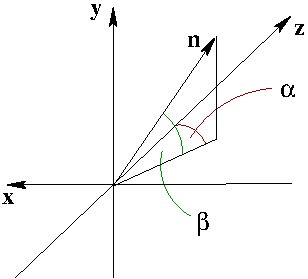
\includegraphics[origin=bl,height=60mm,angle=0]{./figures/rbendangle.pdf}
  %
  \caption{\label{rbendangle}
    Visualisation of angles used to rotate the face compared to the incoming beam. n is the normal of the face.
  }
  %
  \end{center}
%
\end{figure}

\subsection{\opalcycl mode}

This is a restricted feature: \noopalcycl .

\section{Quadrupoles}
\label{sec:quadrupole}
\index{QUADRUPOLE}
\begin{verbatim}
label:QUADRUPOLE,TYPE=string,APERTURE=real-vector,
          L=real,K1=real,K1S=real;
\end{verbatim}
A \texttt{QUADRUPOLE} has three real attributes:
\begin{description}
\item[L]
  \index{L}
  The quadrupole length (default: 0~m).
  A \secref{thin quadrupole}{thin} is defined by setting the length to zero. This is not valid for \opalt or \opalcycl.
\item[K1]
  \index{K1}
  The normal quadrupole component
  $K_1=\frac{1}{B \rho}\frac{\partial B_y}{\partial x}$.
  The default is $0 \mathrm{m}^{-2}$.
  The component is positive, if $B_y$ is positive on the positive $x$-axis.
  This implies horizontal focusing of positively charged particles which
  travel in positive $s$ direction.\\
  In \opalt $K_1=\frac{\partial B_y}{\partial x}$.
\item[K1S]
  \index{K1S}
  The skew quadrupole component
  $K_{1s}=\frac{1}{B \rho}\frac{\partial B_x}{\partial x}$.
  The default is $0 \mathrm{m}^{-2}$.
  The component is negative, if $B_x$ is positive on the positive $x$-axis.\\
In \opalt $K_{1s}=\frac{\partial B_x}{\partial x}$.
\end{description}
\noindent Example:
\begin{verbatim}
QF:QUADRUPOLE,L=1.5,K1=0.001;
\end{verbatim}
The reference system for a quadrupole is a 
\figref{Cartesian coordinate system}{straight}.

\subsection{\opalt mode}
\label{sec:quadrupole-t}
Using a quadrupole in OPAL-t mode, the following additional parameters are defined:
\begin{description}
\item[FMAPFN]
  \index{FMAPFN}
  Field maps in the {\em T7} format can be specified. This field map has to be of type \texttt{3DMagnetoStatic} or \texttt{1DMagnetoStaticEnge}. The latter type is used to calculate the Enge coefficients of the fringe fields. With help of this Enge coefficients the fringe field is constructed. Not yet implemented.
\item[ELEMEDGE]
  \index{ELEMEDGE}
  The edge of the field is specified absolute (floor space co-ordinates) in m.
  \end{description}
\noindent Example:
\begin{verbatim}
QP1: Quadrupole, L=1.20, ELEMEDGE=-0.5265, 
          FMAPFN="1T1.T7", K1=0.11;
\end{verbatim}

\subsection{\opalcycl mode}

This is a restricted feature:  \noopalcycl .

\section{Sextupoles}
\label{sec:sextupole}
\index{SEXTUPOLE}
\begin{verbatim}
label: SEXTUPOLE,TYPE=string,APERTURE=real-vector,
           L=real,K2=real,K2S=real;
\end{verbatim}
A \texttt{SEXTUPOLE} has three real attributes:
\begin{description}
\item[L]
  \index{L}
  The sextupole length (default: 0~m).
  A \secref{thin sextupole}{thin} is defined by setting the length to zero.
\item[K2]
  \index{K2}
  The normal sextupole component
  $K_2=\frac{1}{B \rho}\frac{\partial^2 B_y}{\partial x^2}$.
  The default is $0 \mathrm{m}^{-3}$.
  The component is positive, if $B_y$ is positive on the positive $x$-axis.
\item[K2S]
  \index{K2S}
  The skew sextupole component
  $K_{2s}=\frac{1}{B \rho}\frac{\partial^2 B_x}{\partial x^2}$.
  The default is $0 \mathrm{m}^{-3}$.
  The component is negative, if $B_x$ is positive on the positive $x$-axis.
\end{description}
\noindent Example:
\begin{verbatim}
S:SEXTUPOLE,L=0.4,K2=0.00134;
\end{verbatim}
The reference system for a sextupole is a 
\figref{Cartesian coordinate system}{straight}.
\subsection{\opalt mode}

\subsection{\opalcycl mode}

This is a restricted feature: \noopalt, \noopalcycl .

\section{Octupoles}
\label{sec:octupole}
\index{OCTUPOLE}
\begin{verbatim}
label:OCTUPOLE,TYPE=string,APERTURE=real-vector,
          L=real,K3=real,K3S=real;
\end{verbatim}
An \texttt{OCTUPOLE} has three real attributes:
\begin{description}
\item[L]
  \index{L}
  The octupole length (default: 0~m).
  A \secref{thin octupole}{thin} is defined by setting the length to zero.
\item[K3]
  \index{K3}
  The normal sextupole component
  $K_3=\frac{1}{B \rho}\frac{\partial^3 B_y}{\partial x^3}$.
  The default is $0 \mathrm{m}^{-4}$.
  The component is positive, if $B_y$ is positive on the positive $x$-axis.
\item[K3S]
  \index{K3S}
  The skew sextupole component
  $K_{3s}=\frac{1}{B \rho}\frac{\partial^3 B_x}{\partial x^3}$.
  The default is $0 \mathrm{m}^{-4}$.
  The component is negative, if $B_x$ is positive on the positive $x$-axis.
\end{description}
\noindent Example:
\begin{verbatim}
O3:OCTUPOLE,L=0.3,K3=0.543;
\end{verbatim}
The reference system for an octupole is a 
\figref{Cartesian coordinate system}{straight}.
\subsection{\opalt mode}

\subsection{\opalcycl mode}

This is a restricted feature: \noopalt, \noopalcycl .

\section{General Multipoles}
\label{sec:multipole}
\index{MULTIPOLE}
A \texttt{MULTIPOLE} is thin lens of arbitrary order, including a dipole:
\begin{verbatim}
label:MULTIPOLE,TYPE=string,APERTURE=real-vector,L=real,
      KNORMAL=real-vector,KSKEW=real-vector;
\end{verbatim}
\begin{description}
\item[L]
  \index{L}
  The multipole length (default: 0~m).
  A \secref{thin multipole}{thin} is defined by setting the length to zero.
\item[KN]
  \index{KN}
  A \secref{real vector}{anarray},
  containing the normal multipole coefficients.
  A component is positive, if $B_y$ is positive on the positive $x$-axis.
\item[KS]
  \index{KS}
  A \secref{real vector}{anarray},
  containing the skew multipole coefficients.
  A component is negative, if $B_x$ is positive on the positive $x$-axis.
\end{description}
The multipole coefficients are defined as
$K_{n} = \frac{1}{B \rho}\frac{\partial^n B_y}{\partial x^n}$.
(default: $0 \mathrm{m}^{-n}$).
The order $n$ is unlimited,
but all components up to the maximum must be given, even if zero.
The number of poles of each component is ($2 n + 2$).
The most important error components of fully symmetric quadrupoles are:
\texttt{KNORMAL[5]}, the 12-pole, and \texttt{KNORMAL[9]}, 
the twenty-pole.
Superposition of many multipole components is permitted.
The reference system for a multipole is a 
\figref{Cartesian coordinate system}{straight}.

\noindent Example:
\begin{verbatim}
M27:MULTIPOLE,L=1,KNORMAL[3]=0.0001,KSKEW[2]=0.0001;
\end{verbatim}
A multipole with no dipole component has no effect on the reference orbit,
i.e. the reference system at its exit is the same as at its entrance.
If it includes a dipole component,
it has the same effect on the reference orbit as a \texttt{SBEND}
with the same length and deflection angle \texttt{KNORMAL[0]*L}.
\subsection{\opalt mode}

\subsection{\opalcycl mode}

This is a restricted feature: \noopalt, \noopalcycl .

\section{Solenoids}
\label{sec:solenoid}
\index{SOLENOID}
\begin{verbatim}
label:SOLENOID,TYPE=string,APERTURE=real-vector,
          L=real,KS=real;
\end{verbatim}
A \texttt{SOLENOID} has two real attributes:
\begin{description}
\item[L]
  \index{L}
  The length of the solenoid (default: 0~m)
\item[KS]
  \index{KS}
  The solenoid strength $K_s$ (default: 0 rad/m).
  For positive \texttt{KS} and positive particle charge,
  the solenoid field points in the direction of increasing $s$.
\end{description}
\noindent Example:
\begin{verbatim}
SOLO:SOLENOID,L=2.,K=0.001;
\end{verbatim}
The reference system for a solenoid is a 
\figref{Cartesian coordinate system}{straight}.

\subsection{OPAL-t mode}
\label{sec:solenoid-t}
Using a solenoid in OPAL-t mode, the following additional parameters are defined:
\begin{description}
\item[FMAPFN]
  \index{FMAPFN}
  Field maps in the {\em T7} format can be specified.
\item[ELEMEDGE]
  \index{ELEMEDGE}
  The edge of the field is specified absolute (floor space co-ordinates) in m.
  \end{description}
\noindent Example:
\begin{verbatim}
SP1: Solenoid, L=1.20, ELEMEDGE=-0.5265, 
          FMAPFN="1T1.T7", KS=0.11;
\end{verbatim}

\subsection{\opalcycl mode}

This is a restricted feature: \noopalcycl .

\section{Cyclotron}
\label{sec:cyclotron}
\index{CYCLOTRON}
\begin{verbatim}
label:CYCLOTRON,TYPE=string, CYHARMON=int, 
          PHIINIT=real, PRINIT=real, RINIT=real, 
          SYMMETRY=real, RFFREQ=real, FMAPFN=string;
\end{verbatim}
A \texttt{CYCLOTRON} object includes the main characteristics of a cyclotron ,the magnetic field, 
 and also the initial condition of the injected reference particle, and it has currently the following attributes:
\begin{description}
\item[CYHARMON]
  \index{CYHARMON}
  The hamonic number of the cyclotron $h$. 
\item[RFFREQ]
  \index{RFFREQ}
  The first hamonic frequency of the RF system $f_{rf}$  (default: 0 MHz).
  The particle revolation frquency $f_{rev}$ =  $f_{rf}$ / $h$.
\item[FMAPFN]
  \index{FMAPFN}
  Filename for the magnetic field map. 
\item[SYMMETRY]
  \index{SYMMETRY}
  Defines symmetry characteristic of the B field map data stored in the file.  
\item[RINIT]
  \index{RINIT}
  The initial radius of reference particle (default: 0 mm)
\item[PHINIT]
  \index{PHINIT}
  The initial azimuth of reference particle (default: 0 deg)
\item[PRINIT]
  \index{PRINIT}
  Initial radial momenta of reference particle $P_r$=$\beta$$\gamma$ (doefaule : 0)
\end{description}
\noindent Example:
\begin{verbatim}
  ring: Cyclotron, TYPE="RING", CYHARMON=6, PHIINIT=0.0, 
           PRINIT=-0.000240, RINIT=2131.4 , SYMMETRY=8.0, 
           RFFREQ=50.650, FMAPFN="s03av.nar";
\end{verbatim}
The globe reference system for cyclotron is the Cartesian coordinate system.
Time is used as the  independent variable.
This is a restricted feature: \opalcycl .
\section{Orbit Correctors}
\label{sec:corrector}
\index{orbit corrector}
\index{KICKER}
\index{HKICKER}
\index{VKICKER}
Three types of closed orbit correctors are available:
\begin{description}
\item[HKICKER]
  \index{HKICKER}
  \label{sec:hkicker}
  A corrector for the horizontal plane,
\item[VKICKER]
  \index{VKICKER}
  \label{sec:vkicker}
  A corrector for the vertical plane,
\item[KICKER]
  \index{KICKER}
  \label{sec:kicker}
  A corrector for both planes.
\end{description}
\begin{verbatim}
label:HKICKER,TYPE=string,APERTURE=real-vector,
          L=real,KICK=real;
label:VKICKER,TYPE=string,APERTURE=real-vector,
          L=real,KICK=real;
label:KICKER, TYPE=string,APERTURE=real-vector,
          L=real,HKICK=real,VKICK=real;
\end{verbatim}
They have the following attributes:
\begin{description}
\item[L]
  \index{L}
  The length of the closed orbit corrector (default: 0~m).
\item[KICK]
  \index{KICK}
  The kick angle for either horizontal or vertical correctors.
  (default: 0~rad).
\item[HKICK]
  \index{HKICK}
  The horizontal kick angle for a corrector in both planes
  (default: 0~rad).
\item[VKICK]
  \index{VKICK}
  The vertical kick angle for a corrector in both planes
  (default: 0 rad).
\end{description}
A positive kick increases $p_{x}$ or $p_{y}$
respectively.

\noindent Examples:
\begin{verbatim}
HK1:HKICKER,KICK=0.001;
VK3:VKICKER,KICK=0.0005;
KHV:KICKER, HKICK=0.001,VKICK=0.0005;
\end{verbatim}
The first kicker is rotated about the longitudinal axis by 10 degrees.
The reference system for an orbit corrector is a 
\figref{Cartesian coordinate system}{straight}.

\subsection{\opalt mode}

\subsection{\opalcycl mode}

This is a restricted feature: \noopalt, \noopalcycl .

\section{RF Cavities}
\label{sec:cavity}
\index{RFCAVITY}
\index{cavity}
For an \texttt{RFCAVITY} the three modes have four real attributes in common:
\begin{verbatim}
label:RFCAVITY,APERTURE=real-vector,L=real,VOLT=real,LAG=real;
\end{verbatim}
\begin{description}
\item[L]
  \index{L}
  The length of the cavity (default: 0~m)
\item[VOLT]
  \index{VOLT}
  The peak RF voltage (default: 0~MV).
  The effect of the cavity is
  $\delta E=\mathtt{VOLT}\cdot\sin(2\pi(\mathtt{LAG}-\mathtt{HARMON}\cdot f_0 t))$.
\item[LAG]
  \index{LAG}
  The phase lag [$2\pi$] (default: 0).
\end{description}

\subsection{\opalmap mode}
The following attributes are supported only by the \opalmap mode
\begin{description}
\item[HARMON]
  \index{HARMON}
  The harmonic number $h$ (no default).
  Note that the RF frequency is computed from the harmonic number
  and the revolution frequency $f_0$.
  \textbf{The frequency attribute \texttt{FREQ} must no longer be used.}
\item[BETRF]
  \index{BETRF}
  RF coupling factor (default: 0).
\item[PG]
  \index{PG}
  The RF power per cavity (default: 0~mW).
\item[SHUNT]
  \index{SHUNT}
  The relative shunt impedance (default: $0 M\Omega/\mathrm{m}$).
\item[TFILL]
  \index{TFILL}
  The filling time of the cavity $T_\mathrm{fill}$
  (default: $0 \mu\mathrm{s}$).
\end{description}
Use of a cavity requires the particle momentum \texttt{P}
and the particle charge \texttt{CHARGE} to be set on the relevant 
optics command before any calculations is performed.

\noindent Example:
\begin{verbatim}
CAVITY:RFCAVITY,L=10.0,VOLT=150.0,LAG=0.0,HARMON=31320;
       STATIC,P=50.0,PARTICLE=ELECTRON;
\end{verbatim}
The reference system for a cavity is a 
\figref{Cartesian coordinate system}{straight}.

\subsection{\opalt mode}
\label{sec:cavity-t}
Using a RF Cavity in OPAL-t mode, the following additional parameters are defined:
\begin{description}
\item[FMAPFN]
  \index{FMAPFN}
  Field maps in the {\em T7} format can be specified.
\item[ELEMEDGE]
  \index{ELEMEDGE}
  The edge of the field is specified absolute (floor space co-ordinates) in m.
  \item[TYPE]
  \index{TYPE}
  Type specifies STANDING [default] or SINGLE GAP structures.   
  \item[FREQ]
  \index{FREQ}
  Defines the frequency of the RF Cavity in units of MHz. A warning is issued when the frequency of
  the cavity card does not correspond to the frequency defined in the   FMAPFN file. The  frequency of
  the cavity card overrides the  frequency defined in the  FMAPFN file.
  \end{description}
\noindent Example standing wave cavity which mimics a DC gun:
\begin{verbatim}
gun: RFCavity, L=0.018, VOLT=-131/(1.052*2.658), 
     FMAPFN="1T3.T7", ELEMEDGE=0.00, 
     TYPE="STANDING", FREQ=1.0e-6;
\end{verbatim}
\noindent Example of a two frequency standing wave cavity:
\begin{verbatim}
rf1: RFCavity, L=0.54, VOLT=19.961, LAG=193.0/360.0,
     FMAPFN="1T3.T7", ELEMEDGE=0.129, TYPE="STANDING", 
     FREQ=1498.956;
rf2: RFCavity, L=0.54, VOLT=6.250, LAG=136.0/360.0,
     FMAPFN="1T4.T7", ELEMEDGE=0.129, TYPE="STANDING", 
     FREQ=4497.536;
\end{verbatim}

\subsection{\opalcycl mode}
\label{sec:cavity-cycl}
Using a RF Cavity (standing wave) in \opalcycl mode, the following  parameters are defined:
\begin{description}
\item[FMAPFN]
  \index{FMAPFN}
  Defines name of file which stores normalized voltage amplitude curve of cavity gap in ASCII format.
  (See data format in Section\ref{sec:opalcycl:fildmap})
 \item[VOLT]
  \index{VOLT}
  Sets peak value of voltage amplitude curve in MV.
  \item[TYPE]
  \index{TYPE}
  Defines Cavity type, SINGLEGAP represents cyclotron type cavity.   
  \item[FREQ]
  \index{FREQ}
  Sets the frequency of the RF Cavity in units of MHz. 
  \item[RMIN]
  \index{RMIN}
  Sets the radius of the cavity inner edge in mm.
  \item[RMAX]
  \index{RMAX}
  Sets the radius of the cavity outer edge in mm.

  \item[ANGLE]
  \index{ANGLE}
  Sets the azimuthal position of the cavity in global frame in degree. 

  \item[PDIS]
  \index{PDIS}
  Set shift distance of cavity gap from center of cyclotron in mm.
  
  \item[GAPWIDTH]
  \index{GAPWIDTH}
  Set gap width of  cavity in mm.

  \item[PHI0]
  \index{PHI0}
  Set initial phase of cavity in degree.

\end{description}

\noindent Example of a RF cavity of cyclotron:
\begin{verbatim}
rf0: RFCavity, VOLT=0.25796, FMAPFN="Cav1.dat",
      TYPE="SINGLEGAP",FREQ=50.637, RMIN = 350.0,
      RMAX = 3350.0, ANGLE=35.0,   PDIS = 0.0,
      GAPWIDTH = 0.0, PHI0=phi01;
\end{verbatim}

\begin{figure}
  %
  \begin{center}
  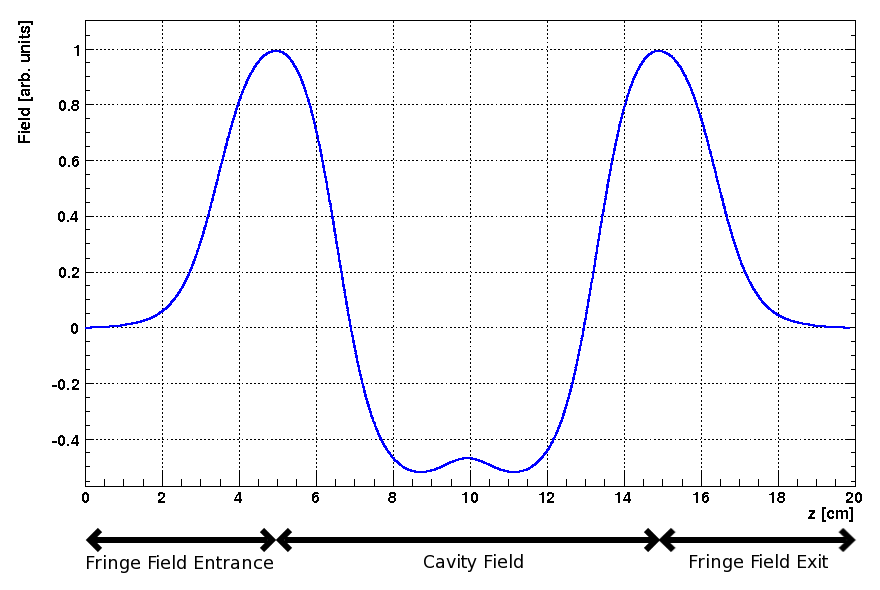
\includegraphics[origin=bl,height=80mm,angle=0]{./figures/traveling-wave-structure/FINSB-RAC-field.png}
  %
  \caption{\label{figure_FINSB-RAC-field}
    The field on axis for an S-band (2997.924~MHz) \texttt{TRAVELINGWAVE} structure. The field of a single cavity
    is shown between its entrance and exit fringe fields. The fringe fields extend $\frac{1}{2}$ wavelength ($\lambda$) to either side.
  }
  %
  \end{center}
%
\end{figure}

\section{Traveling Wave Structure}
\label{sec:travelingwave}
\index{TRAVELINGWAVE}
\subsection{\opalt mode [only]}
An example of a 1D \texttt{TRAVELINGWAVE} structure field map is shown in Figure~\ref{figure_FINSB-RAC-field}.
This map is a standing wave solution generated by Superfish and shows the field on axis for a single accelerating cavity with
the fringe fields of the structure extending to either side. \opalt reads in this field map and constructs the total field of the
\texttt{TRAVELINGWAVE} structure in three parts: the entrance fringe field, the structure fields and the exit fringe field. \\\\

\noindent The fringe fields are treated as standing wave structures and are given by:\\\\
\begin{equation*}
\vec{E_{ent.}}(\vec{r}, t) = \vec{E_{from-map}}(\vec{r}) \cdot VOLT \cdot \cos (2\pi(FREQ \cdot t + \phi_{ent.}))
\end{equation*}
\\
and
\\
\begin{equation*}
	\vec{E_{exit}}(\vec{r}, t) = \vec{E_{from-map}}(\vec{r}) \cdot VOLT \cdot \cos (2\pi(FREQ \cdot t + \phi_{exit}))
\end{equation*}
\\
where VOLT and FREQ are the field magnitude and frequency attributes (see below). 
$ \phi_{ent.}= \text{LAG}$, the phase attribute of the element (see below). $ \phi_{exit} $ is dependent upon both LAG and the NUMCELLS
attribute (see below) and is calculated internally by \opalt.
\\\\
\noindent The field of the main accelerating structure is reconstructed from the center section of standing wave solution shown in
Figure~\ref{figure_FINSB-RAC-field} using
\\
\begin{equation*}
	\begin{split}
	\vec{E}(\vec{r},t)=\frac{VOLT}{\sin (2\pi \cdot MODE)} \lbrace \vec{E_{from-map}}(x,y,z) \cdot \cos(2\pi(FREQ \cdot t \\
		+ \text{LAG} + \dfrac{\pi}{2} \cdot \text{MODE})) \\
		\quad +\vec{E_{from-map}}(x,y,z+d) \cdot \cos(2\pi(FREQ \cdot t\\
		+ \text{LAG} + \dfrac{3\pi}{2} \cdot \text{MODE})) \rbrace
	\end{split}
\end{equation*}
where d is the cell length and is defined as $\text{d} = \lambda \cdot \text{MODE} $. MODE is an attribute of the element (see below).
When calculating the field from the map ($ E_{from-map}(x,y,z) $), the longitudintal position is referenced to the start of the cavity fields
at $ \frac{\lambda}{2} $ (In this case starting at $ z = 5.0 cm $). If the longitudinal position advances past the end of the cavity map
($ \frac{3\lambda}{2} = 15.0 cm $ in this example), an integral number of cavity wavelenths is subtracted from the position until it is back
within the map's longitudinal range. \\

\noindent A \texttt{TRAVELINGWAVE} structure has seven real attributes, one integer attribute, one string attribute and one boolean attribute:
\begin{verbatim}
label:TRAVELINGWAVE,APERTURE=real-vector,L=real,
      VOLT=real,LAG=real, FMAPFN=string, ELEMEDGE=real,
      FREQ=real,NUMCELLS=integer,MODE=real;
\end{verbatim}

\begin{description}
\item[L]
  \index{L}
  The length of the cavity (default: 0~m).
\item[VOLT]
  \index{VOLT}
  The peak RF voltage (default: 0~MV).
  The effect of the cavity is
  $\delta E=\mathtt{VOLT}\cdot\sin(2\pi(\mathtt{LAG}- \mathtt{FREQ}\cdot t))$.
\item[LAG]
  \index{LAG}
  The phase lag [$2\pi$] (default: 0).
\item[FMAPFN]
  \index{FMAPFN}
  Field maps in the {\em T7} format can be specified.
\item[ELEMEDGE]
  \index{ELEMEDGE}
  The edge of the field is specified absolute (floor space co-ordinates) in m. This is the position of the front edge
  of the first \texttt{TRAVELINGWAVE} cavity. (In the simulation the actual field will extend $\frac{1}{2}$ wavelength
  in front of this position.)
\item[FREQ]
  \index{FREQ}
  Defines the frequency of the traveling wave structure in units of MHz. A warning is issued when the frequency of
  the cavity card does not correspond to the frequency defined in the  FMAPFN file. The frequency defined in the FMAPFN
  file overrides the frequency defined on the cavity card. 
\item[NUMCELLS]
  \index{NUMCELLS}
  Defines the number of cells in the tank. (The cell count should not include the entry and exit half cell fringe fields.)
\item[MODE]
  \index{MODE}
Defines the mode in units of $2\pi$, for example $\frac{1}{3}$ stands for a $2\pi\frac{1}{3}$ structure.
\item[FAST]
  \index{FAST}
If FAST is true and the provided fieldmap is in 1D then a 2D fieldmap is constructed from the 1D on-axis field, see section~\ref{sec:fieldmaps}. To track the particles the field values are interpolated from this map instead of using an FFT based algorithm for each particle and each step. (default: FALSE)
\end{description}

\noindent Use of a traveling wave requires the particle momentum \texttt{P}
and the particle charge \texttt{CHARGE} to be set on the relevant 
optics command before any calculations is performed.
\\\\
\noindent Example of a L-Band travelling wave structure:
\begin{verbatim}
lrf0: TravelingWave, L=0.0253, VOLT=14.750, NUMCELLS=40, 
      ELEMEDGE=2.73066, FMAPFN="INLB-02-RAC.Ez", MODE=1/3, 
      FREQ=1498.956, LAG=248.0/360.0;
\end{verbatim}

\section{Electrostatic Separators}
\label{sec:separator}
\index{ELSEPARATOR}
\index{separator}
An \texttt{ELSEPARATOR} (electrostatic separator) has three real
attributes:
\begin{verbatim}
label:ELSEPARATOR,TYPE=string,APERTURE=real-vector,
L=real,EX=real,EY=real;
\end{verbatim}
\begin{description}
\item[L]
  \index{L}
  The length of the separator (default: 0~m).
\item[EX]
  \index{EX}
  The horizontal electric field strength (default: 0~MV/m).
  A positive field increases $p_x$ for positive particles.
\item[EY]
  \index{EY}
  The vertical electric field strength (default: 0~MV/m).
  A positive field increases $p_y$ for positive particles.
\end{description}
A \texttt{ELSEPARATOR} requires the particle momentum \texttt{P} 
and its charge \texttt{CHARGE} to be set in the relevant
\secref{\texttt{BEAM} command}{beam} before any calculations are performed.

\noindent Example:
\begin{verbatim}
BEAM,PARTICLE=POSITRON,PC=46.0;
SEP:ELSEPARATOR,L=5.0,E=0.5;
\end{verbatim}
The reference system for a separator is a 
\figref{Cartesian coordinate system}{straight}.
\subsection{\opalt mode}

\subsection{\opalcycl mode}

This is a restricted feature: \noopalt, \noopalcycl .

\section{Beam Position Monitors}
\label{sec:monitors}
\index{MONITOR}
\index{HMONITOR}
\index{VMONITOR}
A beam monitor acts on the beam like a drift space.
In addition it records the beam position for closed orbit
corrections. 
Four different types of beam position monitors are recognised:
\begin{description}
\item[HMONITOR]
  \label{sec:hmonitor}
  Monitor for the horizontal beam position,
\item[VMONITOR]
  \label{sec:vmonitor}
  Monitor for the vertical beam position,
\item[MONITOR]
  \label{sec:monitor}
  Monitor for both horizontal and vertical beam position.
\item[INSTRUMENT]
  \label{sec:instrument}
  A place holder for any other type of beam instrumentation.
  Optically it behaves like a drift space;
  it returns \textbf{no beam observation}.
  It represents a class of elements
  which is completely independent from drifts and monitors.
\end{description}
\begin{verbatim}
label:HMONITOR,  TYPE=string,APERTURE=real-vecto,L=real;
label:VMONITOR,  TYPE=string,APERTURE=real-vecto,L=real;
label:MONITOR,   TYPE=string,APERTURE=real-vecto,L=real;
label:INSTRUMENT,TYPE=string,APERTURE=real-vector,L=real;
\end{verbatim}
A beam position monitor has one real attribute:
\begin{description}
\item[L]
  \index{L}
  The length of the monitor (default: 0~m). 
  If the length is different from zero,
  the beam position is recorded in the centre of the monitor
  (except for the \texttt{INSTRUMENT} element).
\end{description}
\noindent Examples:
\begin{verbatim}
MH:HMONITOR,L=1;
MV:VMONITOR;
\end{verbatim}
The reference system for a monitor is a 
\figref{Cartesian coordinate system}{straight}.
\subsection{\opalt mode}
Not supported are \texttt{HMONITOR}, \texttt{VMONITOR} and \texttt{INSTRUMENT}. A \texttt{MONITOR} detects all particles passing it and writes the position, the momentum and the time when they hit it into an H5Part file. Furthermore the exact position of the monitor is stored. It has always a length of $1\; cm$ consisting of $0.5\;cm$ drift, the monitor of zero length and another $0.5\;cm$ drift. This is to prevent \opalt from missing any particle. The positions of the particles on the monitor are interpolated from the current position and momentum one step before they would passe the monitor.
\begin{description}
\item[OUTFN]
  \index{OUTFN}
  The filename into which the monitor should write the collected data. The file is an H5Part file.
\item[ELEMEDGE]
  \index{ELEMEDGE}
  The position of the monitor is specified absolute (floor space co-ordinates) in m. This is the position at which the data is collected.
\end{description}

\subsection{\opalcycl mode}

This is a restricted feature:  \noopalcycl .

%\section{Gun}
%\label{sec:gun}
%\index{gun}
%The gun uses the defined distribution (Section \ref{sec:distribution}) and emits particles for a given duration (eventually defined
%by the laser duration).  The temperature is defined by the parameters on the distribution command.

%\begin{verbatim}
%g1:GUN, TYPE=string, TEMISSION=real, L=real, EMISSIONSLICES=real;
%\end{verbatim}
%The gun has beside the standard attribute TYPE,  four more attributes:
%\begin{description}
%\item[L]
%  \index{L}
%  The gun length (default: 0~m).
%\item[TEMISSION]
%  \index{TEMISSION}
%  The time-span  at which emission occurs (default: 0~sec).
%\item[EMISSIONSLICES]
%  \index{EMISSIONSLICES}
%  How many emission slices we consider (default: 0).
%\end{description}

%\noindent Example:
%\begin{verbatim}
%G1:GUN, L=6.0E-3, TEMISSION= 36E-12, EMISSIONSLICES=360;
%\end{verbatim}
%The reference system for a gun is a 
%\figref{Cartesian coordinate system}{straight}.

\section{Collimators}
\label{sec:collimators}
\index{collimator}
\index{ECOLLIMATOR}
\index{RCOLLIMATOR}
Two types of collimators are defined:
\begin{description}
\item[ECOLLIMATOR]
  \label{sec:ecollimator}
  Elliptic aperture,
\item[RCOLLIMATOR]
  \label{sec:rcollimator}
  Rectangular aperture.
\end{description}
\begin{verbatim}
label:ECOLLIMATOR,TYPE=string,APERTURE=real-vector,L=real,
      XSIZE=real,YSIZE=real;
label:RCOLLIMATOR,TYPE=string,APERTURE=real-vector,L=real,
      XSIZE=real,YSIZE=real;
\end{verbatim}
Either type has three real attributes:
\begin{description}
\item[L]
  \index{L}
  The collimator length (default: 0~m).
\item[XSIZE]
  \index{XSIZE}
  The horizontal half-aperture (default: unlimited).
\item[YSIZE]
  \index{YSIZE}
  The vertical half-aperture (default: unlimited).
\end{description}
For elliptic apertures,
\texttt{XSIZE} and \texttt{YSIZE} denote the half-axes respectively,
for rectangular apertures they denote the half-width of the rectangle.
Optically a collimator behaves like a drift space, but during tracking,
it also introduces an aperture limit.
The aperture is checked at the entrance.
If the length is not zero, the aperture is also checked at the exit.

\noindent Example:
\begin{verbatim}
COLLIM:ECOLLIMATOR,L=0.5,XSIZE=0.01,YSIZE=0.005;
\end{verbatim}
The reference system for a collimator is a 
\figref{Cartesian coordinate system}{straight}.


\subsection{\opalt mode}
Not supported at the moment is the \texttt{RCOLLIMATOR}. A \texttt{ECOLLIMATOR} detects all particles which are outside the aperture defined by
\texttt{XSIZE} and \texttt{YSIZE}. The lost particles are saved  into an H5Part file defined by \texttt{OUTFN}.  The \texttt{ELEMEDGE} defines the
location of the collimator and \texttt{L} the length.
\begin{description}
\item[OUTFN]
  \index{OUTFN}
  The filename into which the monitor should write the collected data. The file is an H5Part file.
\item[ELEMEDGE]
  \index{ELEMEDGE}
  The position of the monitor is specified absolute (floor space co-ordinates) in m. This is the position at which the data is collected.
\end{description}

\noindent Example:
\begin{verbatim}
Col:ECOLLIMATOR, L=1.0E-3, ELEMEDGE=3.0E-3, XSIZE=5.0E-4, 
       YSIZE=5.0E-4, OUTFN="Coll.h5";
\end{verbatim}


\subsection{\opalcycl mode}

This is a restricted feature: \noopalcycl .

\section{Coordinate Transformations}
\label{sec:rotation}

\subsection{Rotations About the Vertical Axis}
\label{sec:yrot}
\index{rotation}
\index{coordinate!change}
\index{YROT}
\begin{verbatim}
label:YROT,TYPE=string,APERTURE=real-vector,ANGLE=real;
\end{verbatim}
The element \texttt{YROT} rotates reference system 
\figref{about the vertical ($y$) axis}{yrot}.
\texttt{YROT} has no effect on the beam,
but it causes the beam to be referred to the new coordinate system
\[\begin{array}{lcl}
  x_2&=&x_1\cos\theta-s_1\sin\theta, \\
  y_2&=&x_1\sin\theta+s_1\cos\theta,
\end{array}\]
It has one real attribute:
\begin{description}
\item[ANGLE]
  \index{ANGLE}
  The rotation angle theta (default: 0 rad).
  It must be a \textbf{small} angle,
  i.e. an angle comparable to the transverse angles of the orbit.
\end{description}
A positive angle means that the new reference system is rotated
clockwise about the local $y$-axis with respect to the old system.

\noindent Example:
\begin{verbatim}
KINK:YROT,ANGLE=0.0001;
\end{verbatim}

\subsection{Rotations Around the Longitudinal Axis}
\label{sec:srot}
\index{rotation}
\index{coordinate!change}
\index{SROT}
\begin{verbatim}
label:SROT,TYPE=string,APERTURE=real-vector,ANGLE=real;
\end{verbatim}
The element \texttt{SROT} rotates the reference system
\figref{about the longitudinal ($s$) axis}{srot}.
\texttt{SROT} has no effect on the beam,
but it causes the beam to be referred to the new coordinate system
\[\begin{array}{lcl}
  x_2&=&x_1\cos\psi-y_1\sin\psi, \\
  y_2&=&x_1\sin\psi+y_1\cos\psi,
\end{array}\]
It has one real attribute:
\begin{description}
\item[ANGLE]
  \index{ANGLE}
  The rotation angle psi (default: 0~rad)
\end{description}
A positive angle means that the new reference system is rotated clockwise
about the $s$-axis with respect to the old system.

\noindent Example:
\begin{verbatim}
ROLL1:SROT,ANGLE=PI/2.;
ROLL2:SROT,ANGLE=-PI/2.;
HBEND:SBEND,L=6.0,ANGLE=0.01;
VBEND:LINE=(ROLL1,HBEND,ROLL2);
\end{verbatim}
The above is a way to represent a bend down in the vertical plane,
it could be defined more simply by
\begin{verbatim}
VBEND:SBEND,L=6.0,K0S=-0.01/6.0;
\end{verbatim}

\subsection{General Change of Reference}
\label{sec:patch}
\index{reference!change}
\index{coordinate!change}
\index{PATCH}
\begin{verbatim}
label:PATCH,TYPE=string,APERTURE=real-vector,
	DX=real,DY=real,DZ=real,DTHETA=real,
	DPHI=real,DPSI=real;
\end{verbatim}
The element \texttt{PATCH} applies a general change to the reference system. 
\texttt{PATCH} has no effect on the beam,
but it causes the beam to be referred to the new coordinate system.
It has six real attributes:
\begin{description}
\item[DX]
  \index{DX}
  The displacement in $x$-direction of the new system with respect to the old
  one. 
\item[DY]
  \index{DY}
  The displacement in $y$-direction of the new system with respect to the old
  one. 
\item[DS]
  \index{DS}
  The displacement in $s$-direction of the new system with respect to the old
  one. 
\item[VX]
  \index{VX}
  The rotation around the $x$-axis of the new system with respect to the old
  one. 
\item[VY]
  \index{VY}
  The rotation around the $y$-axis of the new system with respect to the old
  one. 
\item[VZ]
  \index{VZ}
  The rotation around the $s$-axis of the new system with respect to the old
  one. 
\end{description}

\noindent As an example consider a simplified model of the
\figref{separation of the two beams}{patch} near the interaction region of
LHC:
\begin{verbatim}
ALPHA=...;    // The bend angle in the separator magnets.
DISTANCE=...; // The longitudinal distance between
			// the separator magnets.
D1:HKICKER,L=0,KICK=ALPHA;
D2:HKICKER,L=0,KICK=-ALPHA;
DIST:DRIFT,L=DISTANCE;
PATCH1:PATCH,DX=DISTANCE*TAN(ALPHA);
PATCH2:PATCH,DX=-DISTANCE*TAN(ALPHA);
SHARED SEPARATION:LINE=(D1,DIST,D2);
RING1:SEQUENCE,...; // beam goes clockwise.
...
SEPARATION;
PATCH1;             // change reference to 
...
ENDSEQUENCE;
RING2:SEQUENCE,...; // beam goes anticlockwise.
...
SEPARATION;
PATCH2;
...
ENDSEQUENCE;
\end{verbatim}
The direction of travel of each beam determines the signs of the deflections, 
the patches change the reference.
Note that the common reference between the two separator magnets allows a
correct handling of long-distance beam-beam interactions in that area.
\begin{figure}[ht]
  \begin{center}
    \begin{picture}(400,90)
      \thinlines
      \drawline(0,40)(100,40)
      \drawline(100,40)(200,60)(300,60)
      \put(240,65){\vector(1,0){20}}
      \put(305,60){\makebox(0,0)[l]{reference beam 1}}
      \dashline[30]{8}(100,40)(200,40)
      \put(205,40){\makebox(0,0)[l]{common reference}}
      \drawline(100,40)(200,20)(300,20)
      \put(260,15){\vector(-1,0){20}}
      \put(305,20){\makebox(0,0)[l]{reference beam 2}}

      \drawline(100,10)(100,70)
      \put(100,75){\makebox(0,0)[b]{\texttt{D1}}}
      \drawline(200,10)(200,70)
      \put(200,75){\makebox(0,0)[b]{\texttt{D2}+patches}}
    \end{picture}
    \caption{Separation of two beams}
    \label{fig:patch}
  \end{center}
\end{figure}

This is a restricted feature: \noopalt, \noopalcycl .
%
%\section{Beam-Beam Interactions}
%\label{sec:beambeam}
%\index{BEAMBEAM}
%\index{interaction!beam-beam}
%The command \texttt{BEAMBEAM} may be inserted in a beam line
%to simulate a beam-beam interaction point:
%\begin{verbatim}
%label:BEAMBEAM,TYPE=string,APERTURE=real-vector,
%      SIGX=real,SIGY=real,XMA=real,YMA=real,CHARGE=real;
%\end{verbatim}
%The code for this element has been contributed by J.M. Veuillen (1987),
%and has been adapted to C++ in 1997.
%It has six real attributes:
%\begin{description}
%\item[SIGX]
%  \index{SIGX}
%  The horizontal extent (standard deviation) of the opposite beam
%  (default: 0~m).
%\item[SIGY]
%  \index{SIGY}
%  The vertical extent (standard deviation) of the opposite beam
%  (default: 0~m).
%\item[XMA]
%  \index{XMA}
%  The horizontal displacement of the opposite beam with respect to
%  the ideal orbit (default: 0~m).
%\item[YMA]
%  \index{YMA}
%  The vertical displacement of the opposite beam with respect to
%  the ideal orbit (default: 0~m).
%\item[CHARGE]
%  \index{CHARGE}
%  The charge of particles in the opposite beam in proton charges
%  (default: 0).
%\item[NPART]
%  \index{NPART}
%  The number of particles in the opposite beam.
%  (default: 0).
%\end{description}
%A beam-beam element requires the particle momentum \texttt{P}
%and its charge \texttt{CHARGE} to be defined on the relevant optics command
%before any calculations are performed.

%\noindent Example:
%\begin{verbatim}
%BEAM,MOMENTUM=46.0,MASS=PMASS,CHARGE=1.0;
%BB:BEAMBEAM,SIGX=1.E-3,SIGY=5.E-4,CHARGE=1.0,NPART=1.0E12;
%\end{verbatim}

%A three-dimensional representation of a beam-beam interaction is
%available with the command
%\index{BEAMINT}
%\index{interaction!beam-beam}
%\begin{verbatim}
%label:BEAMINT,TYPE=string,APERTURE=real-vector,
%      PHI=real,NSLI=integer,FAST=bool,XIYN=real,DX=real,DY=real,DZ=real,
%      BETXS=real,BETYS=real,ALFXS=real,ALFYS=real,
%      DXS=real,DPXS=real,DYS=real,DPYS=real,
%      EXS=real,EYS=real,SIGTS=real,SIGES=real;
%\end{verbatim}
%Its parameters are:
%\begin{description}
%\item[PHI]
%  \index{PHI}
%  Horizontal crossing angle.
%\item[NSLI]
%  \index{NSLI}
%  Number of slices to be taken in strong beam.
%\item[FAST]
%  \index{FAST}
%  If true, use tables for computing the error function.
%\item[XIYN]
%  \index{XIYN}
%  Beam-beam parameter.
%\item[DX]
%  \index{DX}
%  Horizontal displacement of the interaction point in [m].
%\item[DY]
%  \index{DY}
%  Vertical displacement of the interaction point in [m].
%\item[DZ]
%  \index{DZ}
%  Longitudinal displacement of the interaction point in [m].
%\end{description}
%The following parameters describe the strong beam:
%\begin{description}
%\item[BETXS]
%  \index{BETXS}
%  Horizontal $\beta*$ in [m].
%\item[BETYS]
%  \index{BETYS}
%  Vertical $\beta*$ in [m].
%\item[ALFXS]
%  \index{ALFXS}
%  Horizontal $\alpha*$* in [1].
%\item[ALFYS]
%  \index{ALFYS}
%  Vertical $\alpha*$ in [1].
%\item[DXS]
%  \index{DXS}
%  Horizontal dispersion in [m].
%\item[DPXS]
%  \index{DPXS}
%  Horizontal dispersion slope in [m].
%\item[DYS]
%  \index{DYS}
%  Vertical dispersion in [m].
%\item[DPYS]
%  \index{DPYS}
%  Vertical dispersion slope in [m].
%\item[EXS]
%  \index{EXS}
%  Horizontal emittance in [m rad].
%\item[EYS]
%  \index{EYS}
%  Vertical emittance in [m rad].
%\item[SIGTS]
%  \index{SIGTS}
%  Bunch length in [m].
%\item[SIGES]
%  \index{SIGES}
%  Energy spread in [1].
%\end{description}  

\section{Editing Element Definitions}
\label{sec:elm-edit}
\index{element!editing}
\index{edit!element}
An element definition can be changed in two ways:
\begin{description}
\item[Entering a new definition]
  The element definition will be replaced.
  A beam element, \secref{\texttt{LINE}}{line}, 
  or \secref{\texttt{SEQUENCE}}{sequence}
  can be replaced by another beam element, beam line, or sequence;
  if the replaced item occurs in another beam line or sequence,
  all references in that line or sequence are replaced.
\item[Entering the element name together with new attributes]
  The element will be updated in place,
  and the new attribute values will replace the old ones.
  When the type of the element should not change,
  replacement of an attribute is the more efficient way.
\end{description}
Element definitions can be changed freely.
The changes do not affect already defined objects which belong to
its \secref{class}{elm-class}.
This example shows two ways to change the strength of a quadrupole:
\begin{verbatim}
QF:QUADRUPOLE,L=1,K1=0.01; // Original definition of QF
QF:QUADRUPOLE,L=1,K1=0.02; // Replace whole definition of QF
QF,K1=0.02;                // Replace value of K1
\end{verbatim}
\subsection{\opalt mode}

\subsection{\opalcycl mode}

This is a restricted feature: \noopalt, \noopalcycl .

\section{Wake Functions}
Three types of wake functions are implemented so far: transverse and longitudinal geometric wakes and the CSR wake. The general input format is
\begin{verbatim}
label:WAKE, TYPE=string,NBIN=real,CONST_LENGTH=bool,
      CONDUCT=string,Z0=real,FORM=string,RADIUS=real,
      SIGMA=real,TAU=real,FILTERS=string-array
\end{verbatim}
CONST\_LENGTH, CONDUCT, Z0, FORM, RADIUS, SIGMA and TAU are only used in the geometric wakes.
\begin{description}
\item[TYPE]
  \index{TYPE}
  The type of wake function; either TRANSV-SHORT-RANGE, LONG-SHORT-RANGE or 1D-CSR.
\item[NBIN]
  \index{NBIN}
  Not implemented yet; Number of bins to be used for line density if different from space charge solver grid.
\item[CONST\_LENGTH]
  \index{CONST\_LENGTH}
  
\item[CONDUCT]
  \index{CONDUCT}

\item[Z0]
  \index{Z0}

\item[FORM]
  \index{FORM}

\item[RADIUS]
  \index{RADIUS}

\item[SIGMA]
  \index{SIGMA}

\item[TAU]
  \index{TAU}

\item[FILTERS]
  \index{FILTERS}
  Array of names of filters to be applied onto the longitudinal histogram of the bunch to get rid of the noise and to calculate derivatives. All the filters/smoothers are applied to the line density in the order they appear in the array. The last filter is also used for calculating the derivatives. The actual filters have to be defined elsewhere.
\end{description}

\section{Filters}
Filters can be defined which then are applied to the line density of the bunch. The following smoothing filters are implemented: Savitzky-Golay, Stencil, FixedFFTLowPass, RelativFFTLowPass. The input format for them is
\begin{verbatim}
label:FILTER, TYPE=string, NFREQ=real, THRESHOLD=real, 
      NPOINTS=real, NLEFT=real, NRIGHT=real, 
      POLYORDER=real
\end{verbatim}
\begin{description}
\item[TYPE]
  \index{TYPE}
  The type of filter: Savitzky-Golay, Stencil, FixedFFTLowPass, RelativFFTLowPass
\item[NFREQ]
  \index{NFREQ}
  Only used in FixedFFTLowPass: the number of frequencies to keep
\item[THRESHOLD]
  \index{THRESHOLD}
  Only used in RelativeFFTLowPass: the minimal strength of frequency compared to the stronges to consider.
\item[NPOINTS]
  \index{NPOINTS}
  Only used in Savitzky-Golay: width of moving window in number of points
\item[NLEFT]
  \index{NLEFT}
  Only used in Savitzky-Golay: number of points to the left
\item[NRIGHT]
  \index{NRIGHT}
  Only used in Savitzky-Golay: number of points to the right
\item[POLYORDER]
  \index{POLYORDER}
  Only used in Savitzky-Golay: polynomial order to be used in least square approximation
\end{description}
The Savitzky-Golay filter and the ones based on the FFT routine provide a derivative on a natural way. For the Stencil filter a second order stencil is used to calculate the derivative.

An implementation of the Savitzky-Golay filter can be found in the Numerical Recipes. The Stencil filter uses the following two stencil consecutively to smooth the line density:
$$f_i = \frac{7\cdot f_{i-4} + 24\cdot f_{i-2} + 34\cdot f_{i} + 24\cdot f_{i+2} + 7\cdot f_{i+4}}{96}$$
and
$$f_i = \frac{7\cdot f_{i-2} + 24\cdot f_{i-1} + 34\cdot f_{i} + 24\cdot f_{i+1} + 7\cdot f_{i+2}}{96}.$$
For the derivative a standard second order stencil is used:
$$f^{\prime}_i = \frac{f_{i-2} - 8\cdot f_{i-1} + 8\cdot f_{i+1} - f_{i+2}}{h}$$
This filter was designed by Ilya Pogorelov for the ImpactT implementation of the CSR 1D model.

The FFT based smoothers calculate the Fourier coefficients of the line density. Then they set all coefficients corresponding to frequencies above a certain threshold to zero. Finally the back-transformation is calculate using this coefficients. The two filters differ in the way they identify coefficients which should be set to zero. FixedFFTLowPass uses the n lowest frequencies whereas RelativeFFTLowPass searches for the coefficient which has the biggest absolut value. All coefficients which, compared to this value, are below a threshold (measure in percents) are set to zero. For the derivative the coefficients are multiplied with the following function (this is equivalent to a convolution): 
$$g_{i} = 
\begin{cases}
i \frac{2\pi \imath}{N\cdot L} & i < N/2 \\
-i \frac{2\pi \imath}{N\cdot L} & i > N/2
\end{cases}$$
where $N$ is the total number of coefficients/sampling points and L is the length of the bunch.
\index{element|)}

\chapter{Beam Lines, Sequences, and Ranges}
\label{chp:lines}
\index{line|(}

\section{Beam Lines}
\label{sec:line}
\index{LINE}

The accelerator to be studied is known to \opal
as a sequence of physical elements called a \textbf{beam line}.
A beam line is built from simpler beam lines whose definitions
can be nested to any level.
A powerful syntax allows to repeat or to reflect pieces of beam lines.
Formally a beam line is defined by a \texttt{LINE} command:
\begin{verbatim}
label:LINE=(member,...,member);
\end{verbatim}
\secref{\texttt{label}}{label} gives a name to the beam line 
for later reference.

Each \texttt{member} may be one of the following:
\begin{itemize}
\item An element label,
\item A beam line label,
\item A \secref{\texttt{SEQUENCE}}{sequence} label,
\item A sub-line, enclosed in parentheses,
\end{itemize}
Beam lines can be nested to any level.

\subsection{Simple Beam Lines}
\label{sec:simple}
The simplest beam line consists of single elements:
\begin{verbatim}
label:LINE=(member,...,member);
\end{verbatim}
Example:
\begin{verbatim}
L:LINE=(A,B,C,D,A,D);
TWISS,LINE=L;
\end{verbatim}
The \secref{\texttt{TWISS} command}{twiss} tells \opal to perform
lattice calculations on the sequence 
\begin{verbatim}
A,B,C,D,A,D
\end{verbatim}

\subsection{Sub-lines}
\label{sec:subline}
Instead of referring to an element,
a beam line member can refer to another beam line
defined in a separate command.
This provides a shorthand notation for sub-lines which occur
several times in a beam line.
Lines and sub-lines can be entered in any order,
but when a line is used,
all its sub-lines must be known.

Example:
\begin{verbatim}
L:LINE=(A,B,S,B,A,S,A,B);
S:LINE=(C,D,E);
TWISS,LINE=printL;
\end{verbatim}
This example produces the following expansion steps:
\begin{enumerate}
\item Replace sub-line \texttt{S}:
\begin{verbatim}
(A,B,(C,D,E),B,A,(C,D,E),A,B)
\end{verbatim}
\item Omit parentheses:
\begin{verbatim}
A,B,C,D,E,B,A,C,D,E,A,B
\end{verbatim}
\end{enumerate}

\subsection{Reflection and Repetition}
\label{sec:refrep}
An unsigned repetition count and an asterisk indicate
repetition of a beam line member.
An optional minus sign (\texttt{-}) prefix causes reflection,
i.e. all elements in the subsequence are taken in reverse order.
Sub-lines of reflected lines are also reflected,
but on physical elements the reflection flag is ignored.
The minus sign must precede any repetition count.
Repetitions are expanded immediately when a line is read,
so are reflections of anonymous beam lines.
The result is a flat line referring to a sequence of named elements and/or
beam lines.
Please note this is not yet supported for \noopalt and \noopalcycl .
When the line is output, it has the form resulting from this expansion.

Example:
\begin{verbatim}
R:LINE=(G,H);
S:LINE=(C,R,D);
T:LINE=(2*S,2*(E,F),-S,-(A,B));
TWISS,LINE=T;
\end{verbatim}
The three lines are stored as follows:
\begin{verbatim}
R:LINE=(G,H);
S:LINE=(C,R,D);
T:LINE=(S,S,E,F,E,F,-S,B,A);
\end{verbatim}
When \texttt{T} is expanded, substitution is recursive:
\begin{enumerate}
\item Replace sub-line \texttt{S}:
\begin{verbatim}
(C,R,D,C,R,D,E,F,E,F,D,-R,C,B,A)
\end{verbatim}
\item Replace sub-line \texttt{R}:
\begin{verbatim}
(C,G,H,D,C,G,H,D,E,F,E,F,D,H,G,C,B,A)
\end{verbatim}
\end{enumerate}
Note that the inner sub-line R is reflected together with
the outer sub-line S.
\index{line|)}

\section{Beam Line Sequences}
\label{sec:sequence}
\index{SEQUENCE}
\index{sequence|(}
A sequence of elements can easily be generated from a data base
using a command looking like
\begin{verbatim}
label:SEQUENCE,REFER=keyword,L=expression,REFPOS=name;
   object-definition;
   ...;
   object-definition;
ENDSEQUENCE;
\end{verbatim}
It reads a sequence of element definitions,
compiles an object which resembles a beam line definition,
and gives it the name "label".
The resulting sequence can be used like a beam line.
Please note this is not yet supported for \noopalt and \noopalcycl .
The attributes of the sequence are:
\begin{description}
\item[REFER]
  \index{REFER}
  The reference points for the elements are specified by the \texttt{REFER} 
  attribute:
  \begin{description}
  \item[REFER=CENTRE]
    \index{CENTRE}
    The reference points are at the element centres (default).
  \item[REFER=ENTRY]
    \index{ENTRY}
    The reference points are at element entrances.
  \item[REFER=EXIT]
    \index{EXIT}
    The reference points are at element exits.
  \end{description}
\item[L]
  \index{L}
  The length of the \texttt{SEQUENCE} can be given on the 
  \texttt{SEQUENCE} command,
  or it may be entered with the \texttt{ENDSEQUENCE} command.
\item[REFPOS]
  \index{REFPOS}
  Normally, the reference position for a nested sequence is defined by
  the \texttt{REFER} attribute of the enclosing sequence,
  but, if \texttt{REFPOS} is given, it specifies a \textbf{unique}
  element in the sequence whose \texttt{AT} attribute becomes the 
  reference point for the sequence.
\end{description}
For each non-drift element in the sequence one element definition appears
following the \texttt{SEQUENCE} command and preceding the
\texttt{ENDSEQUENCE} command. 
These look similar to ordinary \chpref{element definitions}{element},
but they may contain an optional specification to place the element:
\begin{verbatim}
class-name,AT=expression;
class-name,AT=expression,FROM=name;
class-name,DRIFT=expression;

object-name,class-name,
	AT=expression,attribute,...,attribute;
object-name,class-name,
	AT=expression,FROM=name,attribute,...,attribute;
object-name,class-name,
	DRIFT=expression,attribute,...,attribute;
\end{verbatim}
The meaning of the \texttt{AT} specifications is:
\begin{description}
\item[AT=expression]
  \index{AT}
  Place the element's entrance, centre, or exit at the specifiet
  position.
\item[FROM=name]
  \index{FROM}
  Interpret the \texttt{AT} specification as relative to the
  \textbf{unique} element \texttt{name}.
\item[FROM=\#S]
  \index{\#S}
  Like omitting the \texttt{FROM} specification, \texttt{AT} is
  relative to the beginning of the sequence.
\item[FROM=\#E]
  \index{\#E}
  The \texttt{AT} specification is relative to the end of the
  sequence. 
\item[FROM=PREVIOUS]
  \index{PREVIOUS}
  The \texttt{AT} specification is relative to the previous element.
\item[FROM=NEXT]
  \index{NEXT}
  The \texttt{AT} specification is relative to the following element.
\item[DRIFT=expression]
  \index{DRIFT}
  The element is preceded by a drift of the given length.
\end{description}

One should consider the following:

\begin{enumerate}
\item The name \texttt{class-name} must be an element 
  \secref{class name}{elm-class}, 
  it may optionally be preceded by a minus sign (\texttt{-}).
  This  inverts the order of the elements in the inserted object.
  This makes sense only for a beam line or sequence.
  
\item If the name \texttt{object-name} is not given,
  \opal inserts the element specified by \texttt{class-name}.
  In this case no further attributes are allowed.
  
\item If there is a non-blank \texttt{object-name},
  this name should not be defined earlier in the data.
  \opal then first makes a copy of \texttt{class-name} and gives it 
  the new name \texttt{object-name}.
  Any further attributes override the attributes inherited from 
  \texttt{class-name}.b
  
\item The elements must be entered in order of increasing position,
  and they must not overlap.
  Their positions are evaluated while reading the \texttt{SEQUENCE}
  definition, and become \textbf{constant} values.
  
\item A \secref{\texttt{LINE}}{line} or
  \secref{\texttt{SEQUENCE}}{sequence} can be nested in another
  \texttt{SEQUENCE} or \texttt{LINE}. 
\end{enumerate}

Within the \texttt{SEQUENCE}, 
\opal generates the drift spaces for proper positioning.

Example:
\begin{verbatim}
// Define element classes for a simple cell:
B:  SBEND,L=35.09,ANGLE = 0.011306116;
QF: QUADRUPOLE,L=1.6,K1=-0.02268553;
QD: QUADRUPOLE,L=1.6,K1=0.022683642;
SF: SEXTUPOLE,L=0.4,K2=-0.13129;
SD: SEXTUPOLE,L=0.76,K2=0.26328;
// Define the cell as a sequence:
CELL:SEQUENCE,L=79.0;
   B1: B, AT=19.115;
   SF1:SF,AT=37.42;
   QF1:QF,AT=38.70;
   B2: B, AT=58.255,ANGLE=-B1->ANGLE;
   SD1:SD,AT=76.74;
   QD1:QD,AT=78.20;
ENDSEQUENCE;
\end{verbatim}
In this example all members of the sequence have a new name,
and \opal generates copies of the corresponding classes.
The bending magnet \texttt{B1} is wrapped to change sign,
but its definition is still equal to \texttt{B}.
Thus \texttt{B2}, which has the negative field of \texttt{B1},
has the same effect as the wrapped element \texttt{B1}.
\index{sequence|)}

\section{Lines and Sequences with arguments}
\index{line!argument}
\index{sequence!argument}
\index{argument!line}
\index{argument!sequence}
A line or sequence definition can also have parameters like a
\secref{\texttt{MACRO}}{macro}.
Such a line or sequence can be nested (and instantiated) in another
line or sequence, but it \textbf{must have a unique name} when
instantiated in a sequence. 
\par
Examples:
\begin{verbatim}
CELL(X,Y):SEQUENCE,L=79;
   QF&X: QF,AT=...;            
   Y&X:  Y,L=1,AT=...;
   QD&X: QD,AT=...;
ENDSEQUENCE;
\end{verbatim}
When used as
\begin{verbatim}
CELL12: CELL(12,SF);
\end{verbatim}
this expands to
\begin{verbatim}
CELL12:SEQUENCE,L=79;
   QF12: QF,AT=...;            
   SF12: SF,L=1,AT=...;
   QD12: QD,AT=...;
ENDSEQUENCE;
\end{verbatim}
A second example:
\begin{verbatim}
CELL(X,Y):LINE=(D1,QF&X,D2,Y&X,D3,QD&X,D4);
\end{verbatim}
If the proper drifts are used, this example is equivalent to
the sequence example above.

\section{Shared Lines}
\label{sec:seq-class}
\index{line!shared}
\index{share lines}
\index{sequence!shared}
\index{shared sequences}
Please note this is not yet supported for \noopalt and \noopalcycl .
Normally, when a beam line or sequence is referred to in another line,
each reference refers to a \textbf{distinct} copy of the line.
\begin{verbatim}
L:LINE=(A,B,C);
S:SEQUENCE,L=real;
   ...
ENDSEQUENCE;
\end{verbatim}
Such a line or sequence is cloned when it is inserted in another line
or sequence, thus permitting assignment of errors to its elements
without affecting other occurrences of the same line.

A beam line or sequence can be shared by using the keyword
\texttt{SHARED},
\index{SHARED}
then the line or sequence is unique,
and all references in other lines refer to the \textbf{same} instance.
Example:
\begin{verbatim}
// Define the interaction region common to both rings:
SHARED IR2:SEQUENCE,L=...;
   ...
ENDSEQUENCE;
RING1:LINE=(...,IR2,...);
RING2:LINE=(...,IR2,...);
// Now assign imperfections to IR2 wich 
// will be seen by both rings:
EALIGN,LINE=IR2,DX=...,DY=...;
\end{verbatim}
Counterexample:
\begin{verbatim}
// Define one superperiod of the machine:
SUPER:SEQUENCE,L=...;
   ...
ENDSEQUENCE;
// Each occurrence of SUPER is distinct:
RING:LINE=(8*SUPER);
// Assign different imperfections to each SUPER:
EALIGN,LINE=RING,DX=...,DY=...;
\end{verbatim}

\section{Sequence Editor}
\label{sec:editor}
\index{edit!sequence}
\index{sequence editor|(}
\index{SEQEDIT}
\index{ENDEDIT}
Please note this is not yet supported for \noopalt and \noopalcycl .
During editing of a sequence, all element positions are evaluated 
immediately when defined and stored as \textbf{constant} values.
To modify a sequence it must be selected for editing by the command
\begin{verbatim}
SEQEDIT,SEQUENCE=old-name;
\end{verbatim}
\opal enters editing mode during which it only recognises the 
\tabref{sequence editor commands}{edit},
and makes the sequence \texttt{old-name} the current sequence being edited.
Editing mode is switched off by the command
\begin{verbatim}
ENDEDIT,NAME=new-name;
\end{verbatim}
If \texttt{new-name} is non-blank, it becomes the name of the edited sequence,
otherwise the modified sequence is stored under its old name.

\begin{table}[ht] \footnotesize
  \begin{center}
    \caption{Commands accepted in editor mode}
    \label{tab:edit}
    \begin{tabular}{|p{0.3\textwidth}|p{0.6\textwidth}|}
      \hline
      Command & Purpose \\
      \hline
      \tabline{SELECT}{Select elements to be affected}{editselect}
      \tabline{CYCLE}{Change starting point (cyclic interchange)}{editcycle}
      \tabline{FLATTEN}{Flatten the sequence}{editflat}
      \tabline{INSTALL}{Install new elements}{editinstall}
      \tabline{MOVE}{Move elements}{editmove}
      \tabline{REFLECT}{Reflect the sequence}{editreflect}
      \tabline{REMOVE}{Remove elements}{editremove}
      \tabline{REPLACE}{Replace elements}{editreplace}
      \tabline{ENDEDIT}{Leave sequence edit mode}{editor}
      \hline
    \end{tabular}
  \end{center}
\end{table}

\subsection{Selecting Element(s)}
\label{sec:editselect}
\index{SELECT}
Elements are selected by a command
\begin{verbatim}
SELECT, RANGE=range, CLASS=name, PATTERN=regex,
        FULL=logical, CLEAR=logical;
\end{verbatim}
When the clause \texttt{SELECTED} is used in an editor command, 
that command acts on all elements currently selected.
A selection remains active until it is explicitly turned off by
\begin{verbatim}
SELECT, CLEAR=TRUE;
\end{verbatim}
\index{CLEAR}
or by an \texttt{ENDEDIT} command
\begin{verbatim}
ENDEDIT;
\end{verbatim}
See also details on element \secref{selection}{select}.

\subsection{Change Start Point}
\label{sec:editcycle}
\index{CYCLE}
The command
\begin{verbatim}
CYCLE, START=place;
\end{verbatim}
\index{START}
makes a cyclic interchange of all elements in the current edit
sequence so as to start at the specified \secref{place}{aplace}.
This element should preferrably be a zero-length element like a
\texttt{MARKER}.
All further edit commands refer to the \textbf{new} positions.

\subsection{Flatten the Sequence being Edited}
\label{sec:editflat}
The sequence loaded into the editor can be flattened by the command
\begin{verbatim}
FLATTEN;
\end{verbatim}
This creates a copy of the sequence with all sub-lines and
sub-sequences expanded,
thus allowing changes also to elements within those nested parts.

\subsection{Install an Element}
\label{sec:editinstall}
\index{INSTALL}
New element(s) can be installed in the edited sequence by the commands
\begin{verbatim}
object-name: class-name, AT=at-expression, SELECTED, 
             attributes;
object-name: class-name, AT=at-expression, FROM=place, 
             attributes;
object-name: class-name, AT=at-expression, attributes;
class-name, AT=at-expression, SELECTED;
class-name, AT=at-expression, FROM=place;
class-name, AT=at-expression;
\end{verbatim}
It has the following attributes:
\begin{description}
\item[object\_name]
The name of the element to be installed.
If the object name is given, attributes may also be specified to
override the attributes of the class.
\item[class\_name]
The name of the class from which the element is to be defined.
\item[AT]
  \index{AT}
  The position where to install the element.
\item[FROM]
  \index{FROM}
  Three cases are possible:
  \begin{description}
  \item[SELECTED]
    \index{SELECTED}
    New elements are inserted at \texttt{AT=at-expression} from each
    currently selected element.
  \item[FROM=place]
    A new element is installed at position \texttt{AT=at-expression}
    relative to the (unique) element at \secref{\texttt{place}}{aplace}.
  \item[FROM omitted or blank]
    A new element is installed at the absolute position
    \texttt{AT=at-expression}. 
  \end{description}
  Relative positions may be negative.
\end{description}
The two names \texttt{object-name} and \texttt{class-name} interact 
in the same way as for a \secref{sequence definition}{sequence}.
The reference points for elements is defined by the REFER attribute of the 
\texttt{SEQUENCE}.

\subsection{Move an Element}
\label{sec:editmove}
\index{MOVE}
The commands
\begin{verbatim}
MOVE, SELECTED, BY=by-expression;
MOVE, ELEMENT=place, BY=by-expression;
MOVE, ELEMENT=place, TO=to-expression;
MOVE, ELEMENT=place, TO=to-expression, FROM=from-name;
\end{verbatim}
move element(s) to new location(s).
Three cases are possible:
\begin{description}
\item[SELECTED,BY=by-expression]
  \index{SELECTED}
  All currently selected elements are moved by \texttt{by-expression}.
\item[ELEMENT=place,BY=by-expression]
  \index{ELEMENT}
  \index{BY}
  The (unique) element at \texttt{place} is moved by \texttt{by-expression}.
\item[ELEMENT=place,TO=to-expression]
  \index{TO}
  The (unique) element at \texttt{place} is moved to the absolute position 
  \texttt{to-expression}.
\item[ELEMENT=place,TO=to-expression,FROM=from-name]
  \index{FROM}
  The (unique) element at \secref{\texttt{place}}{aplace} is moved to
  position \texttt{to-expression} relative to element
  \texttt{from-name}.  A relative position may be negative.
\end{description}
Except in the first case, it is an error to move more than one element
with one \texttt{MOVE} command.
The \texttt{MOVE} command must not attempt to change the order of
elements in the sequence;
elements can not ``hop'' over each other.

\subsection{Reflect a Sequence}
\label{sec:editreflect}
\index{REFLECT}
The command
\begin{verbatim}
REFLECT;
\end{verbatim}
reverses the order of all elements in the sequence currently being
edited.
All further editing commands must refer to the \textbf{new} positions.
The sequence members are \textbf{not} reflected.

\subsection{Remove an Element}
\label{sec:editremove}
\index{REMOVE}
One or more element(s) can be removed by the commands
\begin{verbatim}
REMOVE, SELECTED;
REMOVE, ELEMENT=place;
\end{verbatim}
Two cases are possible:
\begin{description}
\item[SELECTED]
  \index{SELECTED}
  Removes all currently selected elements,
\item[ELEMENT=place]
  \index{ELEMENT}
  Removes the single element at \secref{\texttt{place}}{aplace}.
  It is an error of \texttt{name} occurs more than once in the sequence.
\end{description}

\subsection{Replace an Element}
\label{sec:editreplace}
\index{REPLACE}
The commands
\begin{verbatim}
REPLACE, SELECTED, BY=new-name;
REPLACE, ELEMENT=place, BY=new-name;
\end{verbatim}
replace one or more element(s) in the sequence.
Two cases are possible:
\begin{description}
\item[SELECTED]
  \index{SELECTED}
  All currently selected elements are replaced by an occurrence of the
  element \texttt{new-name}.
\item[ELEMENT=old-name]
  \index{ELEMENT}
  The (unique) element at \secref{\texttt{place}}{aplace} is replaced
  by \texttt{new-name}. 
  It is an error if \texttt{old-name} is not unique.
\end{description}
Example:
\begin{verbatim}
REPLACE, ELEMENT=QF15, BY=QF17; // replace one element
\end{verbatim}
\index{sequence editor|)}

\subsection{Example for the Sequence Editor}
\label{sec:editxmpl}
\index{editor examples}
\begin{verbatim} 
SEQ: SEQUENCE, L=79.00;
   B1:  B, AT=19.115;
   SF1: SF, AT=37.42;
   QF1: QF, AT=38.70;
   B2:  B, AT=58.255;
   SD1: SD, AT=76.74;
   QD1: QD, AT=78.20;
END;

B2W:B2,ANGLE=0.1*B2->ANGLE;

EDIT, SEQUENCE=SEQ;
   MOVE, ELEMENT=SF1, TO=-1.27, FROM=QF1;
   MOVE, ELEMENT=SD1, BY=0.01;
   REPLACE, ELEMENT=B2, BY=BS2;
END, NAME=NEWSEQ;
\end{verbatim}
This example moves the two sextupoles and replaces the element \texttt{B2}
by the element \texttt{B2W}.
The effect of the above \texttt{REPLACE} command is equivalent to
\begin{verbatim}
INSTALL, ELEMENT=B2W, AT=0, FROM=B2;
REMOVE, CLASS=B2;
\end{verbatim}
In this example a new element \texttt{B2W} is installed at the position 
of \texttt{B2} and the the latter is removed.
This works, since all positions are evaluated to constants immediately.

\section{Examples of Beam Lines}


\subsection{PSI XFEL OBLA GUN}
\label{sec:oblagun}
\index{OBLA}
\index{GUN}
\begin{fmpage}
\footnotesize
\begin{verbatim} 
Option, TFS=FALSE;
Option, ECHO=FALSE;
Option, PSDUMPFREQ=10;

Title,string="OBLA Gun";

Edes=1.0E-9;
gamma=(Edes+EMASS)/EMASS;
beta=sqrt(1-(1/gamma^2));
\end{verbatim}
\end{fmpage}
\begin{fmpage}
\begin{footnotesize}
\begin{verbatim}
gambet=gamma*beta;
P0 = gamma*beta*EMASS;
brho = (EMASS*1.0e9*gambet) / CLIGHT;

value,{gamma,brho,Edes,beta,gambet};

// L:        physical element length (real)
// KS:       field scaling factor (real)
// FMAPFN:   field file name (string)
// ELEMEDGE: physical start of the element on the floor (real)
SP1: Solenoid, L=1.20, ELEMEDGE=-0.5335, FMAPFN="1T2.T7",
     KS=0.00011;
SP2: Solenoid, L=1.20, ELEMEDGE=-0.399, FMAPFN="1T3.T7", KS=0.0;
SP3: Solenoid, L=1.20, ELEMEDGE=-0.269, FMAPFN="1T3.T7", KS=0.0;

gun: RFCavity, L=0.011, VOLT=-102.28, FMAPFN="1T1.T7", 
     ELEMEDGE=0.00, TYPE="STANDING", FREQ=1.0e-6;

l1:   Line = (gun,sp1,sp2,sp3); 

rf=1498.956e6;  
v0=beta*CLIGHT;
lz  = 6.5E-12*v0;
value,{v0,lz};

Dist1:DISTRIBUTION, DISTRIBUTION=gungauss,
      sigmax=  0.00030, sigmapx=0.0, corrx=0.0,
      sigmay=  0.00030, sigmapy=0.0, corry=0.0,
      sigmat=  lz, sigmapt=1.0, corrt=0.0 , 
      TEMISSION=3.9e-11, NBIN=39, DEBIN=1;

MINSTEPFORREBIN=1000;

Fs1:FIELDSOLVER, FSTYPE=FFT, MX=32, MY=32, MT=32, 
                 PARFFTX=true, PARFFTY=true, PARFFTT=false,
                 BCFFTX=open, BCFFTY=open, BCFFTT=open, 
                 BBOXINCR=1, GREENSF=STANDARD;

beam1: BEAM, PARTICLE=ELECTRON, pc=P0, NPART=50000, 
       BCURRENT=0.008993736, BFREQ=rf, CHARGE=-1;

Select, Line=l1;
track,line=l1, beam=beam1, MAXSTEPS=2000, DT=1.0e-13;
 run, method = "PARALLEL-T", beam=beam1, fieldsolver=Fs1, 
      distribution=Dist1;
endtrack;
Stop;
\end{verbatim}
\end{footnotesize}
\end{fmpage}

Figure \ref{fig:guncomp2} shows the excellent agreement between \impactt and \opalt.

\begin{figure}[ht]
 \begin{center} 
   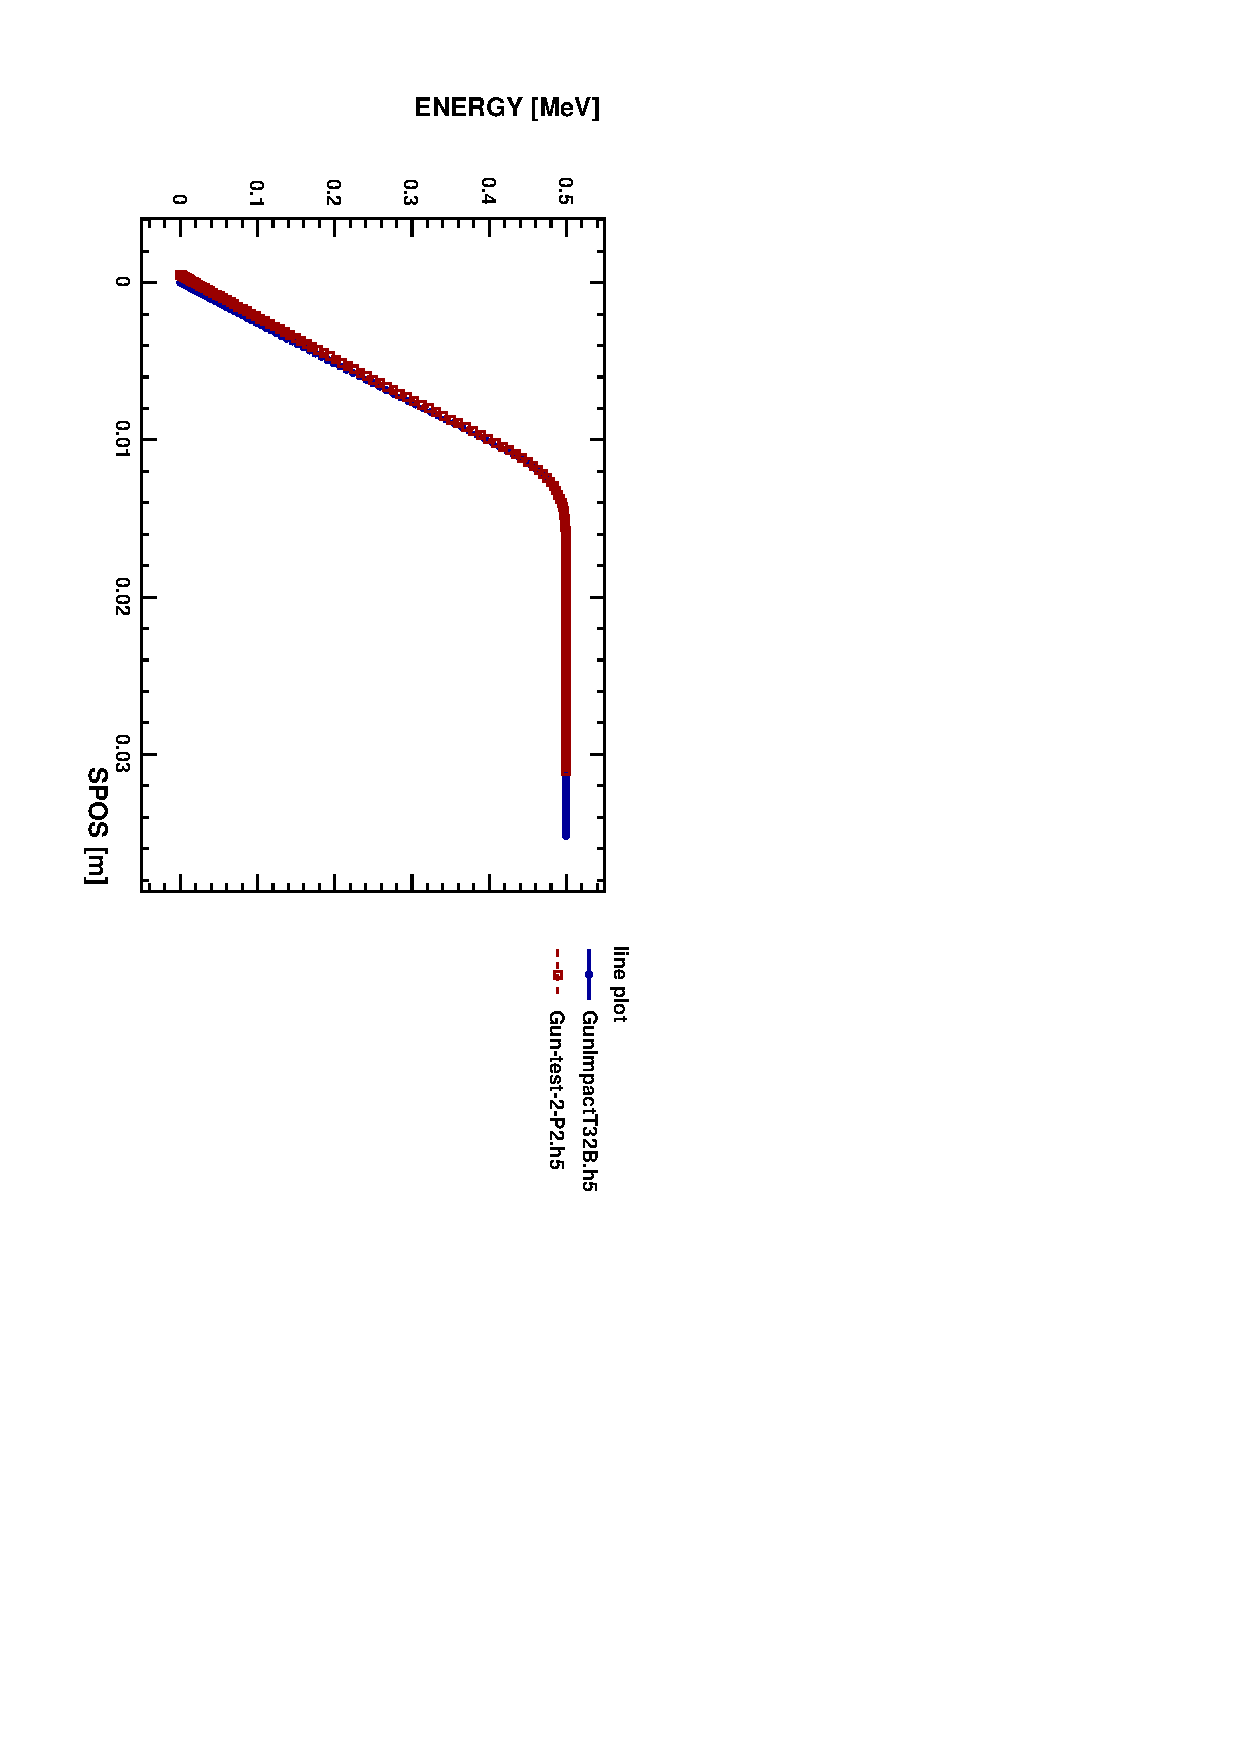
\includegraphics[width=0.6\linewidth,angle=90]{figures/Gun/GunCompEn}
   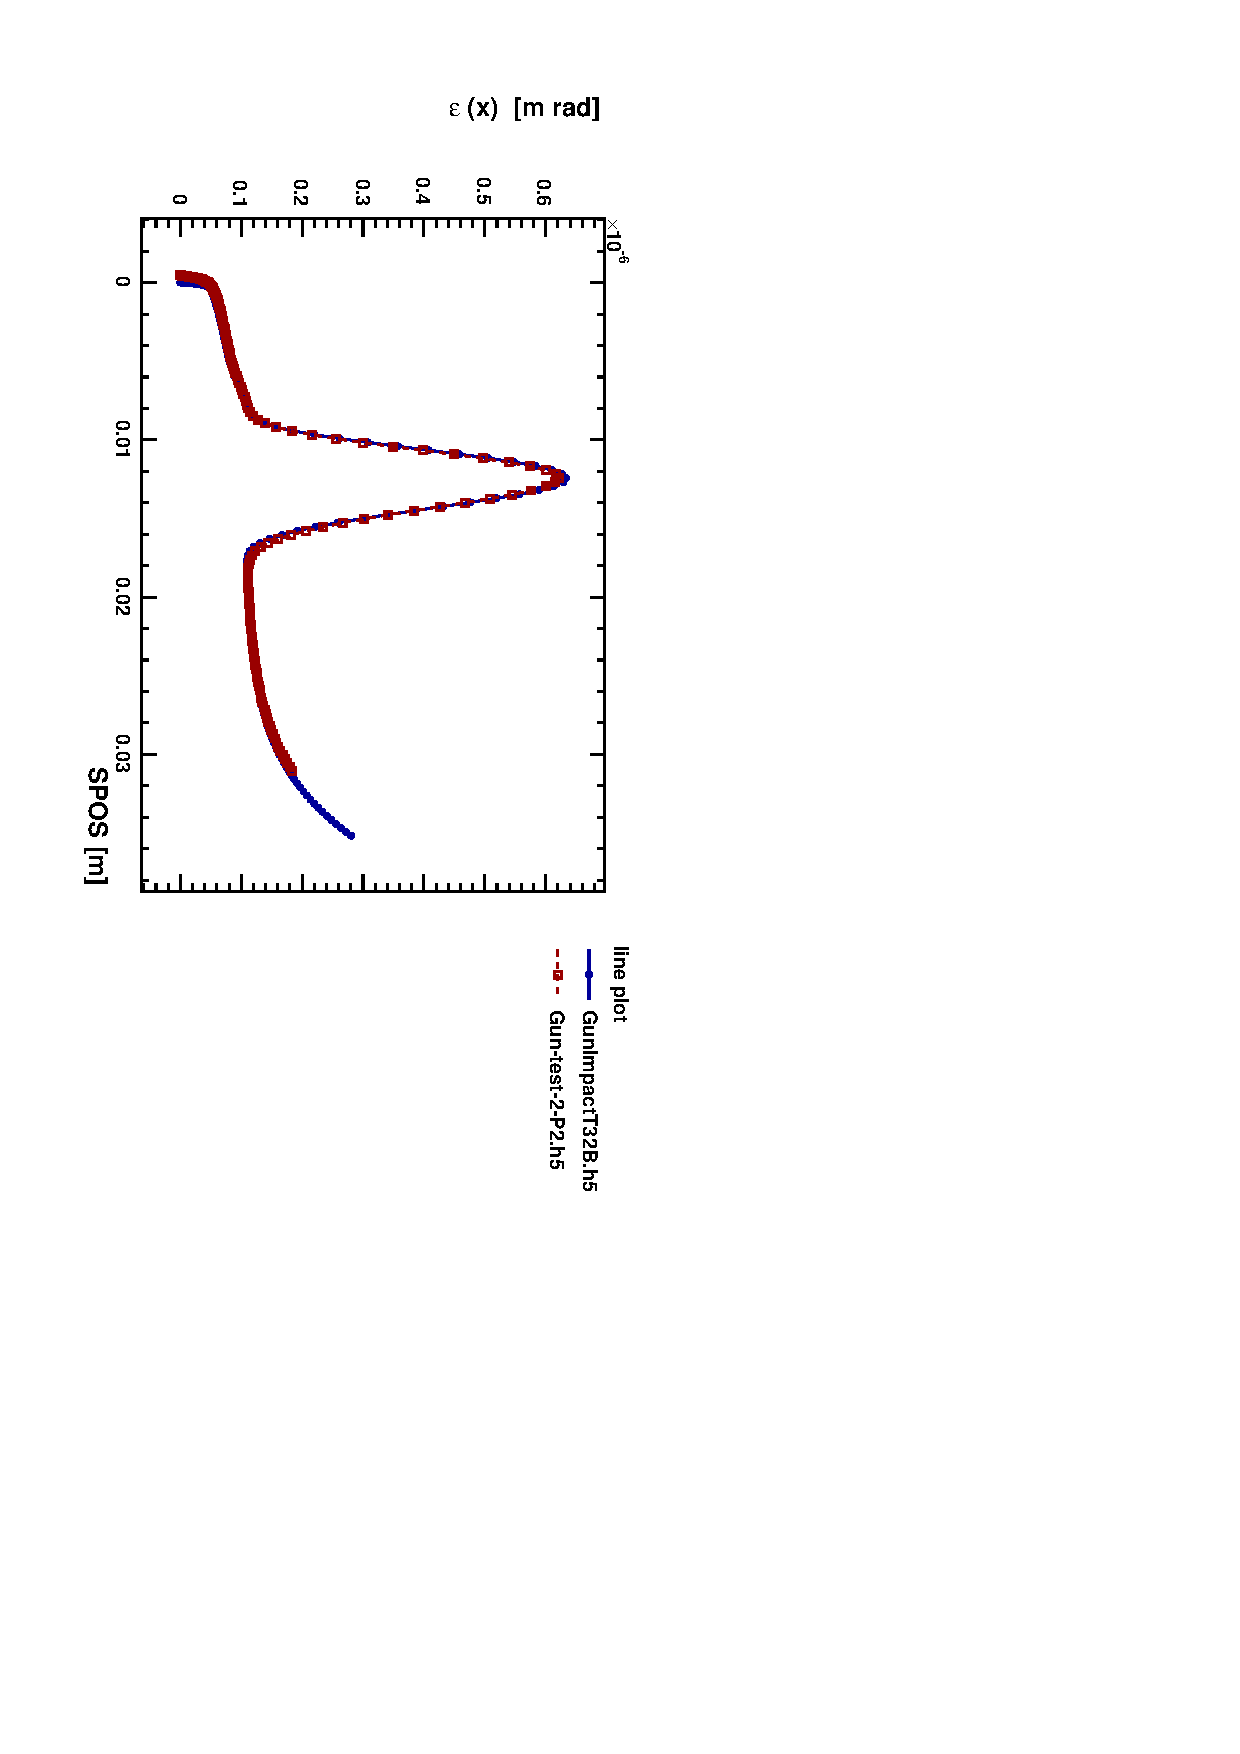
\includegraphics[width=0.6\linewidth,angle=90]{figures/Gun/GunCompEx}
   \caption{Comparison of energy and emittance in $x$ between \impactt and \opalt}   
   \label{fig:guncomp2}
 \end{center}
\end{figure}

\subsection{PSI XFEL 250 MeV Injector}
\label{sec:felinj}
\index{XFEL}
\index{INJECTOR}
\clearpage

\subsection{PSI XFEL 30 MeV Diagnostic Section}
\label{sec:feldiagsec1}
\index{XFEL}
\index{DIAGNOSTIC-1}
\begin{fmpage}
\footnotesize
\begin{verbatim} 
Option, ECHO=FALSE;
Option, TFS=FALSE;
Option, PSDUMPFREQ=10;

Title,string="OPAL Diagnostics test";

Edes=0.0307; //GeV
gamma=(Edes+EMASS)/EMASS;
beta=sqrt(1-(1/gamma^2));
gambet=gamma*beta;
P0 = gamma*beta*EMASS;
brho = (EMASS*1.0e9*gambet) / CLIGHT;
value,{gamma,brho,Edes,beta,gambet};

FINLB02_MSLAC40: Solenoid, L=0.001, KS=0.05, 
                 FMAPFN="FINLB02-MSLAC.T7", ELEMEDGE=4.554;

FIND1_MQ10: Quadrupole, L=0.1, K1=2.788, ELEMEDGE=5.874;
FIND1_MQ20: Quadrupole, L=0.1, K1=-3.517, ELEMEDGE=6.074;


SCREEN: Monitor, L=0.01, ELEMEDGE=7.3867, OUTFN="Screen.h5";

FIND1: Line = (FINLB02_MSLAC40, FIND1_MQ10, FIND1_MQ20, SCREEN);

Dist1:DISTRIBUTION, DISTRIBUTION=gauss,
      sigmax=  1.0e-03, sigmapx=1.0e-4, corrx=0.5,
      sigmay=  2.0e-03, sigmapy=1.0e-4, corry=-0.5,
      sigmat=  3.0e-03, sigmapt=1.0e-4, corrt=0.0;

Fs2:FIELDSOLVER, FSTYPE=FFT, MX=32, MY=32, MT=64, 
    PARFFTX=false, PARFFTY=false, PARFFTT=true,
    BCFFTX=open, BCFFTY=open, BCFFTT=open,
    BBOXINCR=1.0, GREENSF=INTEGRATED;

beam1: BEAM, PARTICLE=ELECTRON, pc=P0, NPART=1e5, 
       BFREQ=1498.953425154e6, BCURRENT=0.299598, CHARGE=-1;

Select, Line=FIND1;

track,line=FIND1, beam=beam1, MAXSTEPS=10000, DT=1.0e-12;
 run, method = "PARALLEL-T", beam=beam1, fieldsolver=Fs2, 
      distribution=Dist1;
endtrack;
Stop;
\end{verbatim}
\end{fmpage}

\subsection{PSI  Injector II Cyclotron}
\label{sec:inj2}
\index{INJECTOR II}
\index{CYCLOTRON}
%%%%%%%%%%
Injector II is a separated sector cyclotron specially designed for preacceleration (inject: $870\,\mathrm{keV}$, extract: $72\,\mathrm{MeV}$ )
of high intensity proton beam for Ring cyclotron. It has 4 sector magnets, two double-gap acceleration cavities 
(represented by 2 single-gap cavities here) and two single-gap flat-top cavities.  

Following is an input file of {\bfseries Single Particle Tracking mode} for PSI Injector II cyclotron.
\begin{fmpage}
\begin{footnotesize}
\begin{verbatim}

// file name ''testinj2-1.in''

Option, TFS=FALSE;
Option, ECHO=FALSE;
Option, PSDUMPFREQ=100000;
Option, SPTDUMPFREQ=5;

Title,string="OPAL-CyclT test";

// define some physical parameters 
Edes=0.002;
gamma=(Edes+PMASS)/PMASS;
beta=sqrt(1-(1/gamma^2));
gambet=gamma*beta;
P0 = gamma*beta*PMASS;
brho = (PMASS*1.0e9*gambet) / CLIGHT;
value,{gamma,brho,Edes,beta,gambet};
phi01= 48.4812-15.0;
phi02=phi01+200.0;
phi03=phi01+1800.0;
phi04=phi01+2000.0;
phi05=(phi01+820.0)*3.0;
phi06=(phi01+2620.0)*3.0;

// define elements and beamline
inj2: Cyclotron, TYPE="Injector2", CYHARMON=10, PHIINIT=30.0, 
      PRINIT=-0.0067, RINIT=392.5, SYMMETRY=1.0, 
      RFFREQ=frequency, FMAPFN="../ZYKL9Z.NAR";

rf0: RFCavity, VOLT=0.25796, FMAPFN="../av1.dat", 
     TYPE="SINGLEGAP", FREQ=frequency, ANGLE=35.0, PHI0=phi01,
     RMIN = 350.0, RMAX = 3350.0, PDIS = 0.0, GAPWIDTH = 0.0; 

rf1: RFCavity, VOLT=0.25796, FMAPFN="../av1.dat", 
     TYPE="SINGLEGAP", FREQ=frequency, ANGLE=55.0, PHI0=phi02, 
     RMIN = 350.0, RMAX = 3350.0, PDIS = 0.0, GAPWIDTH = 0.0; 
\end{verbatim}
\end{footnotesize}
\end{fmpage}
\begin{fmpage}
\begin{footnotesize}
\begin{verbatim}
rf2: RFCavity, VOLT=0.25796, FMAPFN="../av1.dat", 
     TYPE="SINGLEGAP", FREQ=frequency, ANGLE=215.0, PHI0=phi03,  
     RMIN = 350.0, RMAX = 3350.0, PDIS = 0.0, GAPWIDTH = 0.0; 

rf3: RFCavity, VOLT=0.25796, FMAPFN="../av1.dat", 
     TYPE="SINGLEGAP", FREQ=frequency, ANGLE=235.0, PHI0=phi04,  
     RMIN = 350.0, RMAX = 3350.0, PDIS = 0.0, GAPWIDTH = 0.0; 

rf4: RFCavity, VOLT=0.06380, FMAPFN="../av3.dat", 
     TYPE="SINGLEGAP", FREQ=frequency3, ANGLE=135.0, PHI0=phi05,
     RMIN = 830.0, RMAX = 3330.0, PDIS = 0.0, GAPWIDTH = 0.0; 

rf5: RFCavity, VOLT=0.06380, FMAPFN="../av3.dat", 
     TYPE="SINGLEGAP", FREQ=frequency3, ANGLE=315.0, PHI0=phi06, 
     RMIN = 830.0, RMAX = 3330.0, PDIS = 0.0, GAPWIDTH = 0.0; 

l1:   Line = (inj2,rf0,rf1,rf2,rf3,rf4,rf5);

// define particles distribution, read from file
Dist1:DISTRIBUTION, DISTRIBUTION=fromfile, 
      FNAME="PartDatabase.dat"; 

// define fieldsolver, useless for single particle track mode 
Fs1:FIELDSOLVER, FSTYPE=FFT, MX=64, MY=64, MT=64, 
    PARFFTX=true, PARFFTY=true, PARFFTT=false,
    BCFFTX=open, BCFFTY=open, BCFFTT=open;
		 
// define beam parameters
beam1: BEAM, PARTICLE=PROTON, pc=P0, SPACECHARGE=false, 
       NPART=1, BCURRENT=0.0;

// select beamline
Select, Line=l1;

// start tracking
track,line=l1, beam=beam1, MAXSTEPS=106*2000,  STEPSPERTURN=2000;
 run, file = "track_output", turns = 1, method = "CYCLOTRON-T",
      beam=beam1, fieldsolver=Fs1, distribution=Dist1;
endtrack;
Stop;
\end{verbatim}
\end{footnotesize}
\end{fmpage}

To run opal on a single node, just use this command:
{ \footnotesize 
\begin{verbatim}
 opal testinj2-1.in --commlib mpi --info 0 | tee testinj2-1.out
\end{verbatim}
}
Here shows some pictures using the resulting data from single particle tracking using \opalcycl.

Left plot of Figure \ref{fig:Inj2 reference orbit and tune} shows the accelerating orbit of reference particle. After 106 turns, the energy increases from $870\,\mathrm{keV}$ at the injection point to $72.16\,\mathrm{MeV}$ at the deflection point. 
\vspace{0.5cm}
\begin{figure}[ht]
 \begin{center} 
   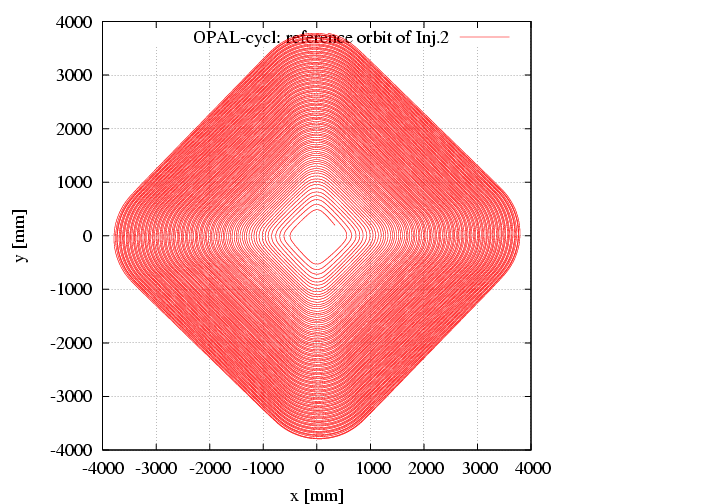
\includegraphics[width=6cm,trim=2.5cm 1.0cm 2.5cm 2.5cm]{figures/cyclotron/AEO_Injector2.png}
    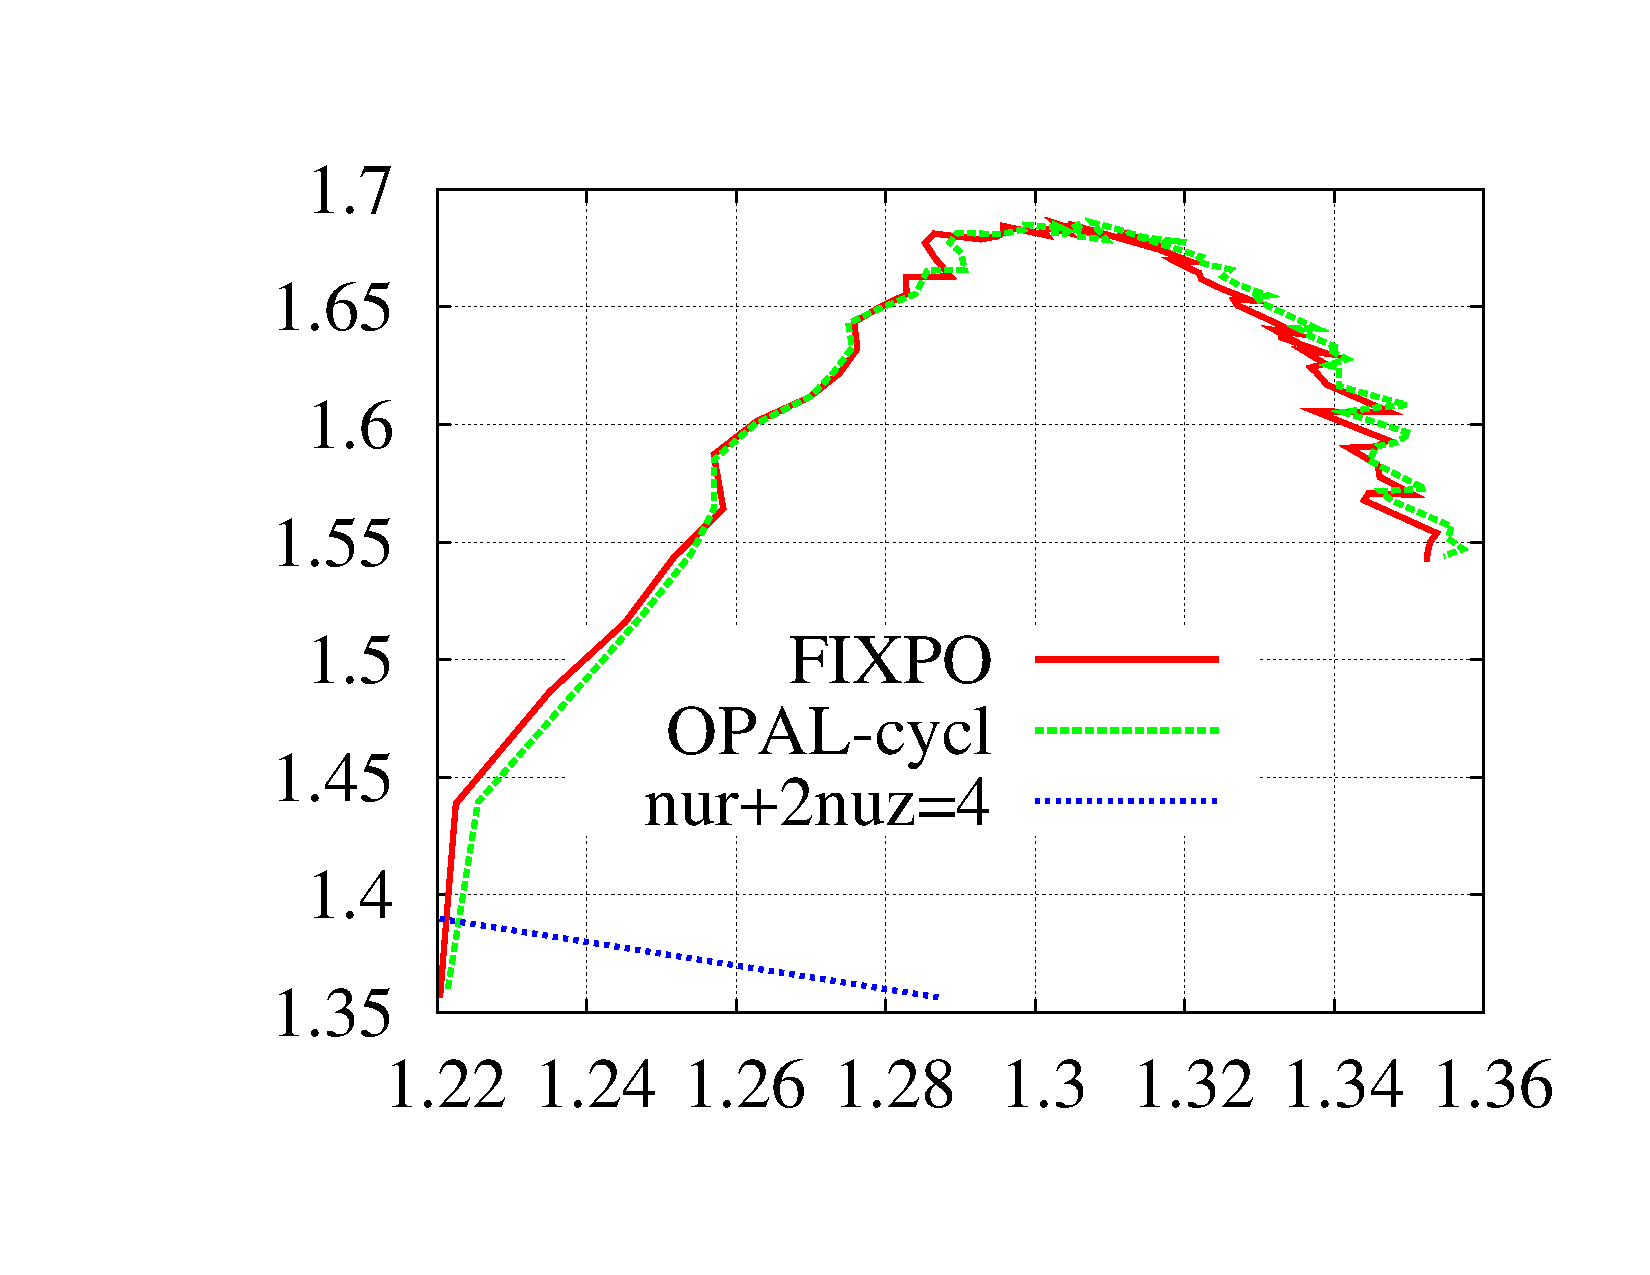
\includegraphics[width=6cm,trim=2.5cm 2.5cm 2.5cm 2.5cm]{figures/cyclotron/nurnuz_Inj2}
    \caption{Reference orbit(left) and tune diagram(right) in Injector II  }
    \label{fig:Inj2 reference orbit and tune}
 \end{center}
\end{figure}

From theoretic view, there should be an eigen ellipse for any given energy in stable area of a fixed accelerator structure. Only when the initial phase space
shape matches its eigen ellipse, the oscillation of beam envelop amplitude will get minimal and the transmission efficiency get maximal.
We can calculate the eigen ellipse by single particle tracking using betatron oscillation property of off-centered particle as following: track 
an off-centered particle and record its coordinates and momenta at the same azimuthal position for each revolution.    
Figure \ref{fig:eigen} shows the eigen ellipse at symmetric line of sector magnet for energy of $2\,\mathrm{MeV}$ in Injector II.
\begin{figure}[ht]
 \begin{center} 
   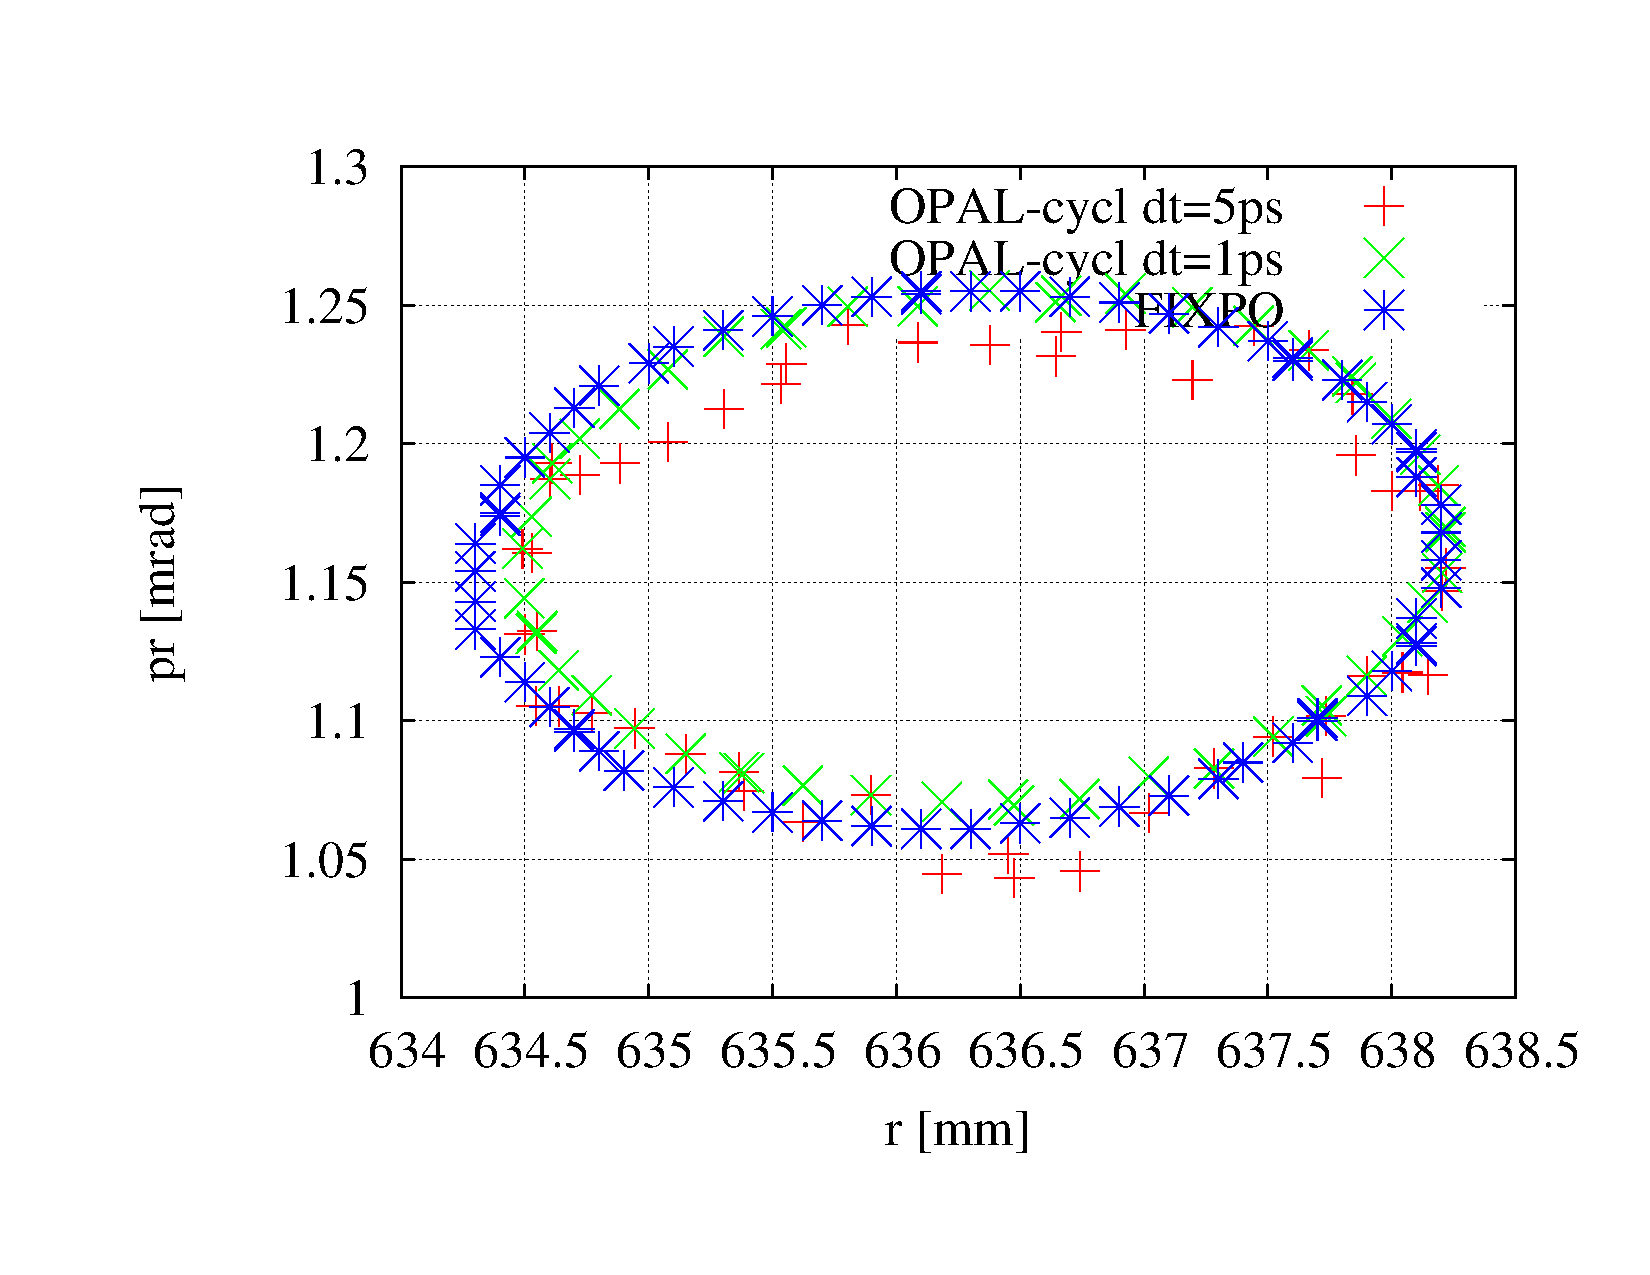
\includegraphics[width=0.45\linewidth,angle=0]{figures/cyclotron/RadialEigen_Inj2}
   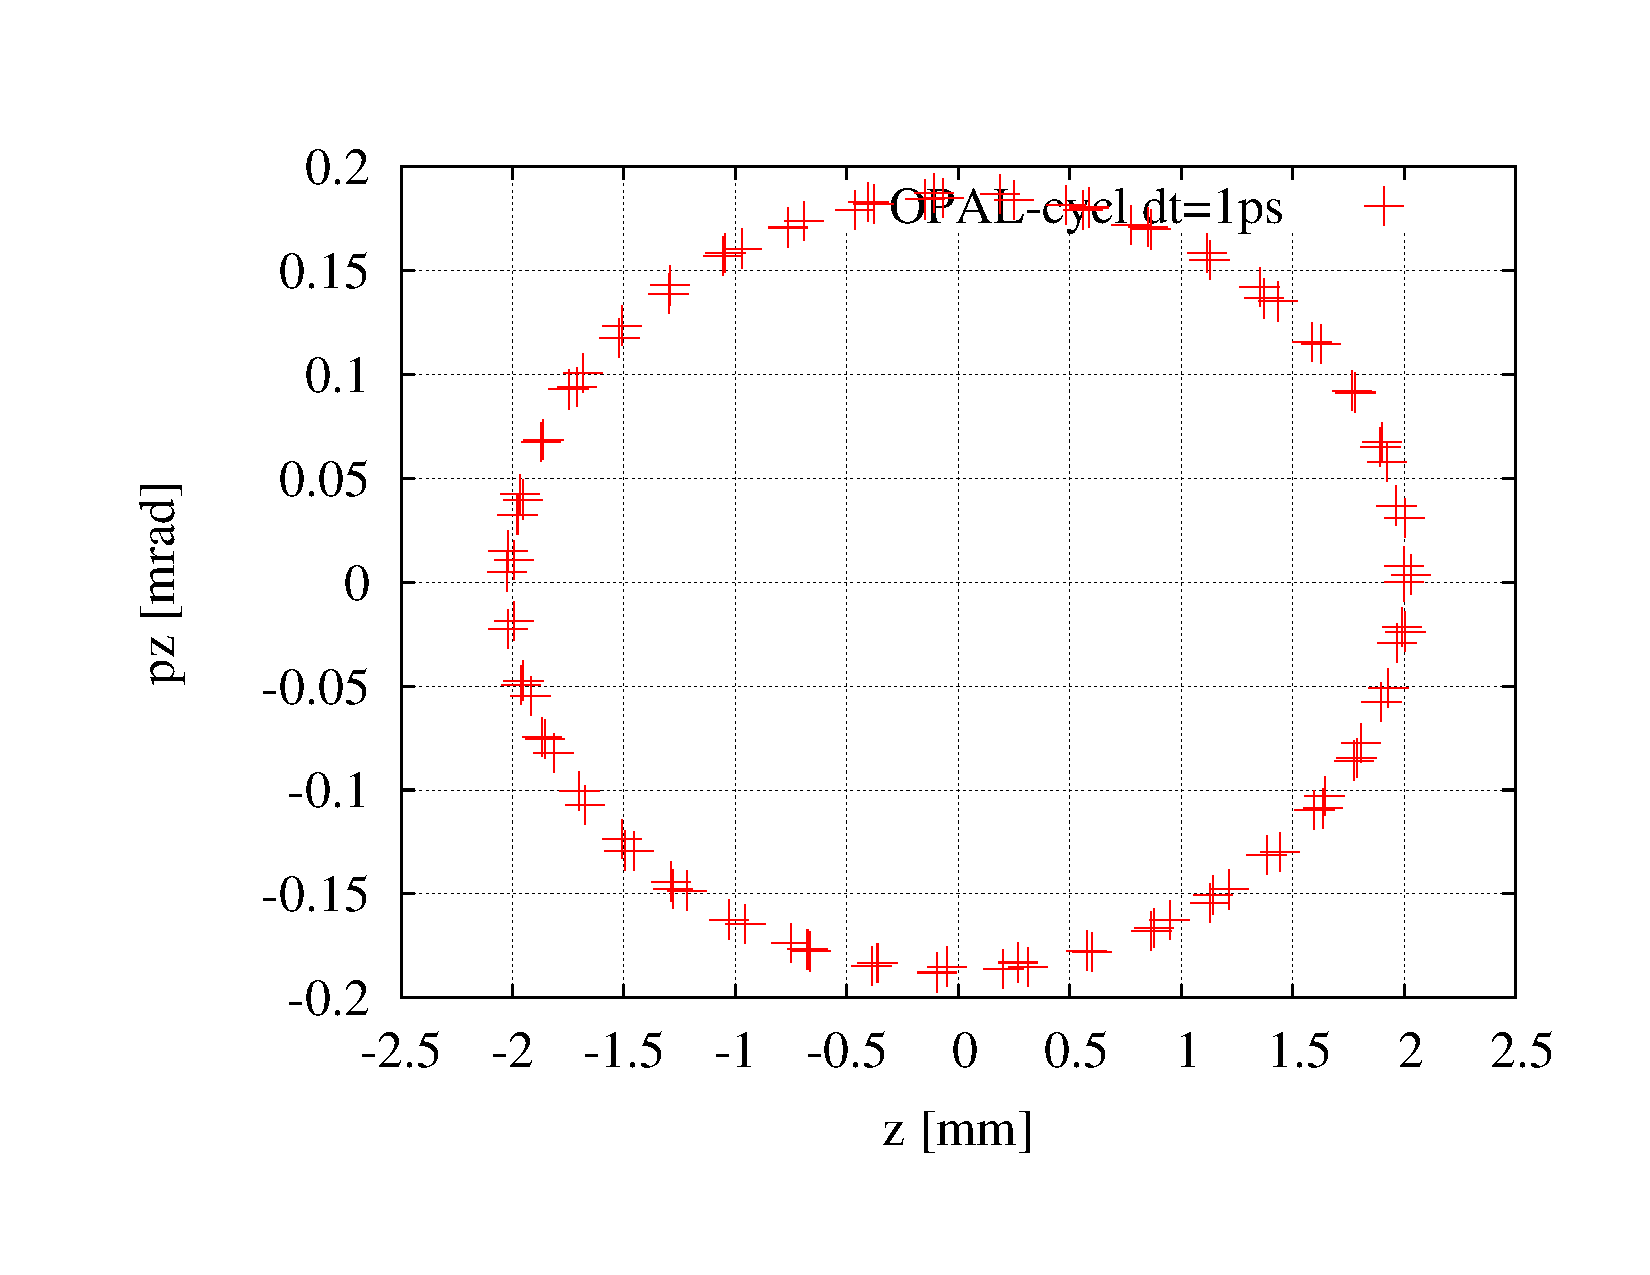
\includegraphics[width=0.45\linewidth,angle=0]{figures/cyclotron/VertEigen_Inj2}
   \caption{Radial and vertical eigenellipse at $2\,\mathrm{MeV}$ of Injector II}   
   \label{fig:eigen}
 \end{center}
\end{figure}
 
Right plot of Figure \ref{fig:Inj2 reference orbit and tune} shows very good agreement of the tune diagram by \opalcycl and FIXPO.
The trivial discrepancy should come from the methods they used.
In FIXPO, the tune values are obtained according to the crossing points of the initially displaced particle. Meanwhile, in \opalcycl, the Fourier 
analysis method is used to manipulate orbit difference between the reference particle and an initially displaced particle.
The frequency point with the biggest amplitude is the betatron tune value at the given energy.

%%%%%%%%%%%%%%
Following is the input file for single bunch tracking with space charge effects in Injector II.
%%%%%%%%%%%%%% 
\begin{fmpage}
\begin{footnotesize}
\begin{verbatim}
 // file name ''testinj2-2.in''
// Define Option parameters 
Option, ECHO=FALSE;
Option, PSDUMPFREQ=10;
Option, SPTDUMPFREQ=5;
Option, REPARTFREQ=10;

// Define title
Title,string="OPAL-CyclT-SC test";

// define some physical parameters 
Edes=0.000870;
gamma=(Edes+PMASS)/PMASS;
beta=sqrt(1-(1/gamma^2));
gambet=gamma*beta;
P0 = gamma*beta*PMASS;
brho = (PMASS*1.0e9*gambet) / CLIGHT;

phi01= 48.4812-15.0;
phi02=phi01+200.0;
phi03=phi01+1800.0;
phi04=phi01+2000.0;
phi05=(phi01+820.0)*3.0;
phi06=(phi01+2620.0)*3.0;

frequency=50.6370;
frequency3=3.0*frequency;

// define elements and beamline
inj2: Cyclotron, TYPE="Injector2", CYHARMON=10, PHIINIT=30.0, 
      PRINIT=-0.0067, RINIT=392.5, SYMMETRY=1.0, 
      RFFREQ=50.6370, FMAPFN="../../ZYKL9Z.NAR";

rf0: RFCavity, VOLT=0.25796, FMAPFN="../../Cav1.dat", 
     TYPE="SINGLEGAP", FREQ=50.637, ANGLE=35.0, PHI0=phi01,
     RMIN = 350.0, RMAX = 3350.0, PDIS = 0.0, GAPWIDTH = 0.0;
\end{verbatim}
\end{footnotesize}
\end{fmpage}
\begin{fmpage}
\begin{footnotesize}
\begin{verbatim}
rf1: RFCavity, VOLT=0.25796, FMAPFN="../../Cav1.dat", 
     TYPE="SINGLEGAP", FREQ=50.637, ANGLE=55.0, PHI0=phi02, 
     RMIN = 350.0, RMAX = 3350.0, PDIS = 0.0, GAPWIDTH = 0.0;

rf2: RFCavity, VOLT=0.25796, FMAPFN="../../Cav1.dat", 
     TYPE="SINGLEGAP", FREQ=50.637, ANGLE=215.0, PHI0=phi03, 
     RMIN = 350.0, RMAX = 3350.0, PDIS = 0.0, GAPWIDTH = 0.0;

rf3: RFCavity, VOLT=0.25796, FMAPFN="../../Cav1.dat", 
     TYPE="SINGLEGAP", FREQ=50.637, ANGLE=235.0, PHI0=phi04,
     RMIN = 350.0, RMAX = 3350.0, PDIS = 0.0, GAPWIDTH = 0.0;

rf4: RFCavity, VOLT=0.06380, FMAPFN="../../Cav3.dat", 
     TYPE="SINGLEGAP", FREQ=151.911, ANGLE=135.0, PHI0=phi05,
     RMIN = 830.0, RMAX = 3330.0, PDIS = 0.0, GAPWIDTH = 0.0;

rf5: RFCavity, VOLT=0.06380, FMAPFN="../../Cav3.dat", 
     TYPE="SINGLEGAP", FREQ=151.911, ANGLE=315.0, PHI0=phi06, 
     RMIN = 830.0, RMAX = 3330.0, PDIS = 0.0, GAPWIDTH = 0.0;

l1:   Line = (inj2,rf0,rf1,rf2,rf3,rf4,rf5);

// define particles distribution, generate Gaussion type
Dist1:DISTRIBUTION, DISTRIBUTION=gauss,
      sigmax=  2.0e-03, sigmapx=1.0e-7, corrx=0.0,
      sigmay=  2.0e-03, sigmapy=1.0e-7, corry=0.0,
      sigmat=  2.0e-03, sigmapt=1.8e-4, corrt=0.0;

// define parallel FFT fieldsolver, parallel in x y direction
Fs1:FIELDSOLVER, FSTYPE=FFT, MX=32, MY=32, MT=32, 
    PARFFTX=true, PARFFTY=true, PARFFTT=false,
    BCFFTX=open, BCFFTY=open, BCFFTT=open,BBOXINCR=5;

// define beam parameters
beam1: BEAM, PARTICLE=PROTON, pc=P0, SPACECHARGE=true,
       NPART=1e5, BCURRENT=3.0E-3, CHARGE=1.0, BFREQ= frequency;

// select beamline
Select, Line=l1;

// start tracking
track,line=l1, beam=beam1, MAXSTEPS=106*2000,  STEPSPERTURN=2000;
 run, file = "track_output", turns = 1, method = "CYCLOTRON-T", 
      beam=beam1, fieldsolver=Fs1, distribution=Dist1;
endtrack;
Stop;
\end{verbatim}
\end{footnotesize}
\end{fmpage}

To run opal on single node, just use this command:
{ \footnotesize 
\begin{verbatim}
 # opal testinj2-2.in --commlib mpi --info 0 | tee testinj2-2.out
\end{verbatim}
}
To run opal on N nodes in parallel environment interactively, use this command instead:
{ \footnotesize 
\begin{verbatim}
 # mpirun -np N opal testinj2-2.in  --commlib mpi 
   --info 0 | tee testinj2-2.out
\end{verbatim}
 }
If restart a job from the last step NSTEP of an existing $.h5$ file, add a new argument like this: 
{ \footnotesize 
\begin{verbatim}
 # mpirun -np N opal testinj2-2.in --restart NSTEP 
   --commlib mpi --info 0 | tee testinj2-2.out
\end{verbatim}
}
Figure \ref{fig:cyclParameters} and \ref{fig:cyclphasespace} are from preliminary simulation results.
They are generated by H5partROOT code.   
\begin{figure}[ht]
  \begin{center} 
    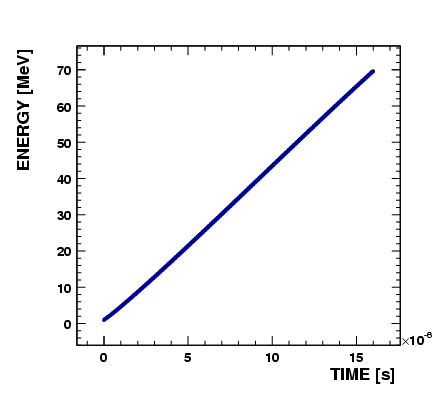
\includegraphics[width=0.45\linewidth]{figures/cyclotron/Inj2-ENERGY-TIME.png}
    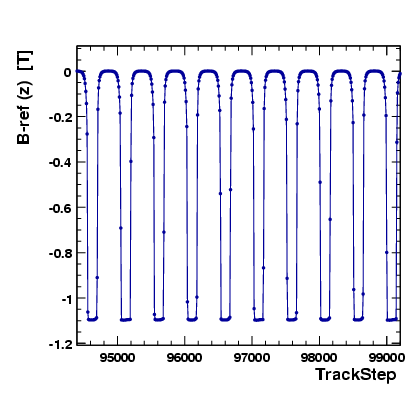
\includegraphics[width=0.45\linewidth]{figures/cyclotron/Inj2-B-ref-z-TrackStep.png}
    \caption{Energy Vs. time (left) and external B field Vs. trackstep (Right, only show for about 2 turns)}
    \label{fig:cyclParameters}
  \end{center}
\end{figure}

\begin{figure}[ht]
  \begin{center} 

    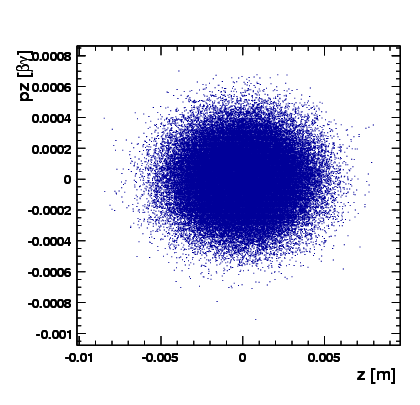
\includegraphics[width=0.3\linewidth]{figures/cyclotron/Inj2-z-pz-step-870KeV.png}
    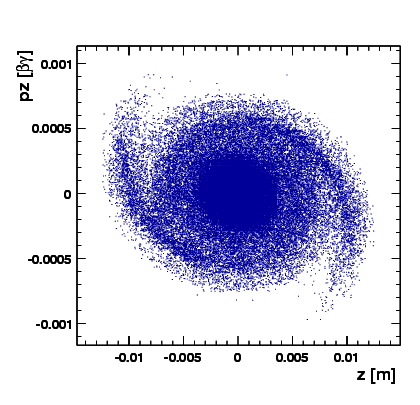
\includegraphics[width=0.3\linewidth]{figures/cyclotron/Inj2-z-pz-step-15MeV.png}
    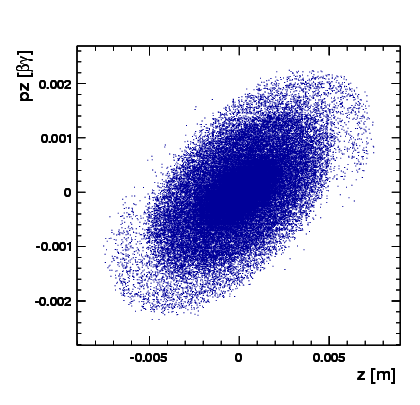
\includegraphics[width=0.3\linewidth]{figures/cyclotron/Inj2-z-pz-step-30MeV.png}
    \caption{Vertical phase at different energy from left to right: $0.87\,\mathrm{MeV}$, $15\,\mathrm{MeV}$ and $35\,\mathrm{MeV}$}
    \label{fig:cyclphasespace}
  \end{center}
\end{figure}

%%%%%%%%%%%%%%
\subsection{PSI  Ring Cyclotron}
\label{sec:Ring}
\index{RING}
\index{CYCLOTRON}
From the view of numerical simulation, the difference between Injector II and Ring cyclotron comes from two aspects:
\begin{description}
\item[B Field] The structure of Ring is totally symmetric, the field on median plain is periodic 
along azimuthal direction, \opalcycl take this advantage to only store 1/8 field data to save memory.

\item[RF Cavity] In the Ring, all the cavities are typically single gap with some parallel displacement from its
radial position.\opalcycl have an argument \texttt{PDIS} to manipulate this issue.  
\end{description}
\begin{figure}[ht]
  \begin{center} 
    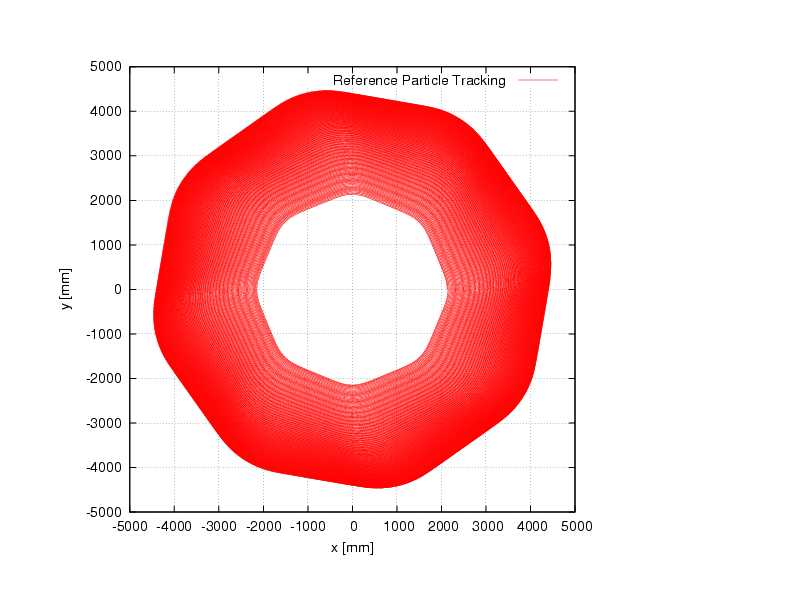
\includegraphics[width=6cm,trim=2.5cm 2.5cm 2.5cm 2.5cm]{figures/cyclotron/AEO_Ring.png}
    \includegraphics[width=6cm,trim=2.5cm 2.5cm 2.5cm 2.5cm]{figures/cyclotron/nurnuz_Ring}
    \caption{Reference orbit(left) and tune diagram(right) in Ring cyclotron }
    \label{fig:Ring reference orbit and tune}
  \end{center}
\end{figure}
Figure \ref{fig:Ring reference orbit and tune} shows a single particle tracking result and tune calculation result in the PSI Ring cyclotron.
Limited by size of the user guide, we don't plan to show too much details as in Injector II.

\clearpage
\subsection{CERN SPS Lattice}
\label{sec:sps}
\index{SPS}
The CERN SPS lattice may be represented using the following beam elements:
\begin{verbatim}
QF:QUADRUPOLE,...; // focusing quadrupole
QD:QUADRUPOLE,...; // defocusing quadrupole
B1:RBEND,...;      // bending magnet of type 1
B2:RBEND,...;      // bending magnet of type 2
DS:DRIFT,...;      // short drift space
DM:DRIFT,...;      // drift space replacing two bends
DL:DRIFT,...;      // long drift space
\end{verbatim}
The SPS machine is represented by the lines
\begin{verbatim}
SPS:   LINE=(6*SUPER);
SUPER: LINE=(7*P44,INSERT,7*P44);
INSERT:LINE=(P24,2*P00,P42);
P00:   LINE=(QF,DL,QD,DL);
P24:   LINE=(QF,DM,2*B2,DS,PD);
P42:   LINE=(PF,QD,2*B2,DM,DS);
P44:   LINE=(PF,PD);
PD:    LINE=(QD,2*B2,2*B1,DS);
PF:    LINE=(QF,2*B1,2*B2,DS);
\end{verbatim}
In order not to overload the example,
small gaps between magnetic elements have been omitted.

\subsection{LEP Lattice}
\label{sec:lep}
\index{LEP}
A preliminary description of LEP has been given in the
\bibref{LEP pink book}{LEP}.
Translation of those element sequences to the \opal input format gives:
\begin{verbatim}
LEP: LINE=(4*SUP);
SUP: LINE=(OCT, -OCT);
OCT: LINE=(LOBS, RFS, DISS, ARC, DISL, RFL, LOBL);
LOBS:LINE=(L1, QS1, L2, QS2, L3, QS3, L4, QS4);
RFS: LINE=(L5, QS5, L5, QS6, L5, 2*(QS7, L5, QS8, L5));
DISS:LINE=(QS11, L25, BW, L22, QS12, L25, B4, L22, QS13, 
           L25, B4, L22, QS14, L25, B4, L31, QS15, L25,
           B4, L32, SF, L23, QS16);
ARC: LINE=(L21, B6, L22, SD, L23, QD,
           7*(CELL(SF1, SD1), CELL(SF, SD)), 
           CELL(SF1, SD1), L24, B6, L41, QF, L21, B6, 
           L22, SD4, L23, QD, 7*(CELL(SF4, SD3), 
           CELL(SF3, SD4)), CELL(SF4, SD3), L24, B6, 
           L22, SF3, L23);
DISL:LINE=(QL16, L34, B4, L22, QL15, L33, B4, L22,
           QL14, L25, B4, L22, QL13, L25, B4, L22, QL12,
           L25, BW, L22, QL11);
RFL: LINE=(2*(L5, QL8, L5, QL7), L5, QL6, L5, QL5, L5);
LOBL:LINE=(QL4, L14, QL3, L13, QL2, L12, QL1, L11);
BW:  LINE=(W, L26, W);
B4:  LINE=(B, L26, B);
B6:  LINE=(B, L26, B, L26,B);
CELL(SF,SD):LINE=(L24, B6, L22, SF, L23, QF, L21, B6,
                  L22, SD, L23, QD);
\end{verbatim}
Here the element definitions have been left out to save space.

\chapter{Physics Commands}
\label{chp:physics}
 
\section{Global Reference Momentum}
\label{sec:P0}
\index{P0}
Before any physics computations are attempted the following command
should be entered:
\begin{verbatim}
P0=real;
\end{verbatim}
This command sets the global reference momentum in GeV/c,
which is used to compute the magnetic fields from the normalised
multipole coefficients.
The \secref{\texttt{BEAM}~command}{beam} then renormalises the
multipole coefficients.
This mechanism allows sending a beam with a momentum different from the
design momentum through a beam line.

\section{BEAM Command}
\label{sec:beam}
\index{BEAM}
All OPAL commands working on a beam require the setting of various
quantities related to this beam. 
These are entered by a \texttt{BEAM} command:
\begin{verbatim}
label:BEAM, PARTICLE=name, MASS=real, CHARGE=real,
      ENERGY=real, PC=real, GAMMA=real, BCURRENT=real,
      EX=real, EXN=real, EY=real, EYN=real, ET=real,
      KBUNCH=integer, NPART=real, BUNCHED=logical,
      RADIATE=logical, DAMP=logical, QUANTUM=logical;
\end{verbatim}
The \texttt{label} is opional, it defaults to \texttt{UNNAMED\_BEAM}.
\index{UNNAMED\_BEAM}
The particle mass and charge are defined by:
\begin{description}
\item{PARTICLE}
  \index{PARTICLE}
  The name of particles in the machine.
  OPAL knows the mass and the charge for the following particles:
  \begin{description}
  \item{POSITRON}
    \index{POSITRON}
    The particles are positrons (\texttt{MASS}=$m_e$,
    \texttt{CHARGE}=1),
  \item{ELECTRON}
    \index{ELECTRON}
    The particles are electrons (\texttt{MASS}=$m_e$,
    \texttt{CHARGE}=-1),
  \item{PROTON}
    \index{PROTON}
    The particles are protons (default, \texttt{MASS}=$m_p$,
    \texttt{CHARGE}=1),
  \item{ANTIPROTON}
    \index{ANTIPROTON}
    The particles are anti-protons (\texttt{MASS}=$m_p$,
    \texttt{CHARGE}=-1).

    \item {HMINUS}
    \index{HMINUS}
    The particles are h- protons (\texttt{MASS}=$m\_{h^{-}}$,
    \texttt{CHARGE}=-1).
    
    \item{CARBON}
     \index{CARBON}
    The particles are carbons (\texttt{MASS}=$m_c$,
    \texttt{CHARGE}=12).
    
      \item{URANIUM}
      \index{URANIUM}
    The particles are of type uranium (\texttt{MASS}=$m_u$,
    \texttt{CHARGE}=35).
         
         \item{MUON}
         \index{MUON}
    The particles are of type muon (\texttt{MASS}=$m_\mu$,
    \texttt{CHARGE}=-1).

   \item{DEUTERON}
     \index{DEUTERON}
    The particles are of type deuteron (\texttt{MASS}=$m_d$,
    \texttt{CHARGE}=1).
    
      \item{XENON}
       \index{XENON}
    The particles are of type xenon (\texttt{MASS}=$m_{xe}$,
    \texttt{CHARGE}=20).
       
  \end{description}
\end{description}
For other particle names one may enter:
\begin{description}
\item{MASS}
  \index{MASS}
  \index{particle!mass}\index{mass}
  The particle mass in GeV.
\item{CHARGE}
  \index{CHARGE}
  \index{particle!charge}\index{charge}
  The particle charge expressed in elementary charges.
\end{description}
By default the particle momentum is \secref{P0}{P0}.
A different value can be defined by one of the following:
\begin{description}
\item{ENERGY}
  \index{ENERGY}
  \index{particle!energy}\index{energy}
  \index{total energy}
  The total energy per particle in GeV.
  If given, it must be greater then the particle mass.
\item{PC}
  \index{PC}
  \index{momentum}
  \index{particle!momentum}
  The momentum per particle in GeV/c.
  If given, it must be greater than zero.
\item{GAMMA}
  \index{GAMMA}
  The ratio between total energy and rest energy of the particles
  $\gamma = E / m_0$.
  If given, it must be greater than one.
  If the mass is changed a new value for the energy should be entered.
  Otherwise the energy remains unchanged,
  and the momentum and $\gamma$ are recalculated.
\end{description}
The emittances are defined by:
\begin{description}
\item{EX}
  \index{EX}
  \index{emittance!horizontal}
  The horizontal emittance
  $E_x=\sigma_x^2/\beta_x$
  (default:~1~m).
\item{EY}
  \index{EY}
  \index{emittance!vertical}
  The vertical emittance
  $E_y=\sigma_y^2/\beta_y$
  (default:~1~m).
\item{ET}
  \index{ET}
  \index{emittance!longitudinal}
  The longitudinal emittance
  $E_t=\sigma_e/(p_0c) \cdot c\sigma_t$
  (default:~1~m).
  The emittances can be replaced
  by the normalised emittances and the energy spread:
\item{EXN}
  \index{EXN}
  \index{normalised emittance}\index{emittance!normalised}
  The normalised horizontal emittance [m]:
  $E_{xn}=4\beta\gamma E_x$
  (ignored if $E_x$ is given).
\item{EYN}
  \index{EYN}
  The normalised vertical emittance [m]:
  $E_{yn}=4\beta \gamma E_y$
  (ignored if $E_y$ is given).
\item{SIGT}
  \index{SIGT}
  \index{bunch!length}
  The bunch length $c\sigma_t$ [m].
\item{SIGE}
  \index{SIGE}
  \index{energy!spread}
  The {\em relative} energy spread $\sigma_e/p_0 c$ [1].
\end{description}
For the time being, only the particle definition
(\texttt{PARTICLE,MASS,CHARGE,PC,
ENERGY,GAMMA}) is used.
The other parameters will be implemented as needed when new commands
become available.
%Certain commands compute the synchrotron tune $Q_s$
%from the RF cavities.
%If $Q_s\neq 0$,
%the relative energy spread $\sigma_e/p_0c$
%and the bunch length $c\sigma_t$ are
%\[
%\frac{\sigma_e}{p_0c}=\sqrt{\frac{2\pi Q_s E_t}{\eta C}},
%\qquad
%c\sigma_t=\sqrt{\frac{\eta C E_t}{2\pi Q_s}},
%\]
%where $C$ is the machine circumference, and
%$\eta = (1/\gamma^2) - (1/\gamma_{tr}^2)$.
%Finally, the \texttt{BEAM} command accepts
%\begin{description}
%\item{KBUNCH}
%  \index{bunch!number}
%  The number of particle bunches in the machine (default:~1).
%\item{NPART}
%  \index{bunch}
%  The number of particles per bunch (default:~0).
%\item{BCURRENT}
%  \index{beam!current}\index{bunch!current}
%  \index{current}
%  The bunch current (default:~0~A).
%\item{BUNCHED}
%  \index{bunch}
%  A logical flag.
%  If set, the beam is treated as bunched whenever this makes sense.
%\item{RADIATE}
%  \index{radiation}
%  \index{synchrotron!radiation}
%  A logical flag.
%  If set, synchrotron radiation is considered in all bipolar magnets.
%\end{description}

\chapter{Tables}
\label{chp:tables}
\index{tables|(}

\section{Introduction}
\label{sec:tabintro}

Please note Tables are not yet supported in \noopalt and \noopalcycl . They probable does not make sense in a non map based computation.  A typical computation in \opal  follows \figref{these steps}{tables}:

\begin{enumerate}
\item
  Define a beam line using a \secref{\texttt{LINE}}{line}
  or \secref{\texttt{SEQUENCE}}{sequence} command.
\item
  Define a beam with using \secref{\texttt{BEAM}}{beam} command.
\item
  If desired, define imperfections on the defined beam line,
  using one of the \chpref{error commands}{error}.
\item
  If desired, attach special integrators to selected elements of the
  defined beam line,
  using \secref{\texttt{SETINTEGRATOR}}{setint} commands.
\item
  If desired, perform an orbit correction on the defined beam line,
  using \secref{\texttt{THREADBPM}}{thread} or
  \secref{\texttt{MICADO}}{micado} command.
\item
  Define a ``Table Object'' using one of the \chpref{table}{tables} commands. 
  This selects a \secref{\texttt{RANGE}}{arange} of a beam line,
  and defines an algorithm to fill the table,
  e.~g. with the lattice functions, 
  the accumulated transfer map from the beginning of the range to the
  current position, or the \secref{\texttt{SURVEY} data}{survey}.
  A table remains in memory and is recomputed as required.
  It is erased only if one of the contained elements or beam lines is changed. 
\item
  If desired, apply the \chpref{match module}{match} to adjust parameters
  in the machine. The match module can work on any number of tables
  simultaneously. 
\item
  Use a \secref{\texttt{LIST}}{list} command to print the contents of any
  table. 
\end{enumerate}

\begin{figure}[ht]
  \begin{center}
    \begin{picture}(400,400)
      \thinlines
      \put(90,370){\vector(0,-1){30}}
      \put(150,370){\vector(0,-1){30}}
      \put(80,310){\framebox(80,30){beam line}}
      \put(210,325){\vector(-1,0){50}}
      \put(240,325){\circle{60}}
      \put(240,325){\makebox(0,0){\shortstack{Error\\Generator}}}
      \put(320,325){\vector(-1,0){50}}
      \put(120,310){\vector(0,-1){30}}
      \put(120,250){\circle{60}}
      \put(120,250){\makebox(0,0){\shortstack{Table\\Generator}}}
      \put(320,250){\vector(-1,0){170}}
      \put(120,220){\vector(0,-1){30}}
      \put(80,160){\framebox(80,30){Table object}}
      \put(210,175){\vector(-1,0){50}}
      \put(240,175){\circle{60}}
      \put(240,175){\makebox(0,0){\shortstack{Match\\Module}}}
      \put(320,175){\vector(-1,0){50}}
      \put(120,100){\circle{60}}
      \put(120,160){\vector(0,-1){30}}
      \put(120,100){\makebox(0,0){\shortstack{Table\\Lister}}}
      \put(320,100){\vector(-1,0){170}}
      \put(120,70){\vector(0,-1){30}}
      \put(80,10){\framebox(80,30){Output}}

      \Thicklines
      \put(20,370){\framebox(80,30){\shortstack{LINE or\\SEQUENCE}}}
      \put(140,370){\framebox(80,30){BEAM}}
      \put(320,310){\framebox(80,30){Error Command}}
      \put(320,235){\framebox(80,30){Table Command}}
      \put(320,160){\framebox(80,30){Match Command}}
      \put(320,85){\framebox(80,30){LIST Command}}
    \end{picture}
    \caption{Schematic view of the Interaction between Objects in \opal}
    \label{fig:tables}
  \end{center}
\end{figure}

\section{Element Selection}
\label{sec:select}
\index{element!selection}
\index{select!element}

Many \opal commands allow for the possibility to process
a subset of the elements occurring in a \chpref{beam line}{lines}.
For this purpose each \chpref{beam line}{lines} and
\chpref{table}{tables} has a selection flag for each element.
The \texttt{SELECT} command may be used to manipulate these flags.
It affects the following commands:
\begin{itemize}
\item \secref{\texttt{EALIGN}}{erroralign},
\item \secref{\texttt{EFIELD}}{errorfield},
\item \secref{\texttt{EFCOM}}{errorfield},
\item \secref{\texttt{EPRINT}}{errorprint},
\item \secref{\texttt{ESAVE}}{errorsave},
\item \secref{\texttt{SURVEY}}{survey},
\item \secref{\texttt{TWISS}}{twiss},
\item \secref{\texttt{ATTLIST}}{attlist},
\item \secref{\texttt{LIST}}{list},
\item \secref{\texttt{EIGEN}}{canned},
\item \secref{\texttt{ENVELOPE}}{canned},
\item \secref{\texttt{MATRIX}}{canned},
\item \secref{\texttt{TWISS3}}{canned}.
\end{itemize}
Three formats are recognised for the command:
\begin{verbatim}
SELECT,LINE=name, FULL;
SELECT,LINE=name, CLEAR;
SELECT,LINE=name, RANGE=range, CLASS=name, TYPE=name,
                PATTERN=regular_expression;
\end{verbatim}
\index{SELECT}
All three forms require the parameter
\begin{description}
\item[LINE]
  \index{LINE}
  The label of a previously defined \chpref{beam line}{lines} or
  \chpref{table}{tables} on which the selection is to be done (no default).
\end{description}
The first format sets the selection flag for all elements in the beam line
and the second format clears the selection flags for all elements.

The third format keeps all existing selections and additionally marks those
elements as selected which belong to the intersection of the following four
sets: 
\begin{description}
\item[RANGE]
  \index{RANGE}
  If \texttt{RANGE} is omitted, the first set contains all elements;
  if it is given, the first set is limited to the named range in the line. 
  The default is equivalent to \texttt{RANGE=\#S/\#E}.
\item[CLASS]
  \index{CLASS}
  The \secref{\texttt{label}}{label} of an element class (default: blank).
  If \texttt{CLASS} is omitted, the second set contains all elements;
  if it is given, the set contains only the elements derived directly or
  indirectly from the named class.
\item[TYPE]
  \index{TYPE}
  If \texttt{TYPE} is omitted, the third set contains all elements;
  if it is given, the set contains only the elements whose \texttt{TYPE}
  attribute is equal to the given name. 
\item[PATTERN]
  \index{PATTERN}
  If \texttt{PATTERN} is omitted, the fourth set contains all elements;
  if it is given, the \secref{\texttt{regular expression}}{wildcard}
  is applied to all element names, and the set contains only the matching
  elements.
\end{description}
The effect of subsequent \texttt{SELECT} commands produces the union of all
selections. 
If a fresh selection is desired, precede the new \texttt{SELECT} command
with the command
\begin{verbatim}
SELECT,LINE=name,CLEAR;
\end{verbatim}
Example:
\begin{verbatim}
SELECT,LINE=X, RANGE=IP1/IP2;                  // (1)
SELECT,LINE=X, CLASS=BB;                       // (2)
SELECT,LINE=X, PATTERN=".*\.L1";               // (3)
SELECT,LINE=X, RANGE=IP1/IP2,CLASS=BB, 
               PATTERN=".*\.L1";               // (4)
SELECT,LINE=LHC, CLASS=IP;                     // (5)
T:TWISS,LINE=LHC;                              // (6)
SELECT,LINE=T ,CLASS=QUADRUPOLE;               // (7)
TWISS3,TABLE=T, FILE=name,TFS;                 // (8)
U:TWISS,LINE=LHC;                              // (9)
\end{verbatim}
Command (1) selects all elements from \texttt{IP}1 to \texttt{IP2}, 
both included.
Command (2) selects all elements in the ring which belong to or are 
derived from class \texttt{BB}.
Command (3) selects all elements in the ring whose names end \texttt{.L1}.
Command (4) is the most restrictive, it selects all elements
between \texttt{IP1} and \texttt{IP2} which are derived from class 
\texttt{BB} and whose names end in \texttt{.L1}.

Command (5) sets the selections flags on all interaction points in
line \texttt{LHC}.
The selection is transmitted to command (6), which generates the
\texttt{TWISS} table \texttt{T} lists the default columns for the
interaction points. 
Command (7) sets additional selection flags on the table \texttt{T}
for all quadrupoles,
and command (8) lists the Mais-Ripken functions for all interaction
points and all quadrupoles.
Command (9) gets the selection from line \texttt{LHC}, i.~e. the
selection concerns only the interaction points.

\section{Attach Special Integrators}
\label{sec:setint}
\index{SETINTEGRATOR}
\index{integrator}

By default the algorithm applied to each element in the machine is
defined by the table command.
It may be overridden for selected elements by applying a \texttt{SETINTEGRATOR}
command to attach a special integrator.
It has the form
\begin{verbatim}
SETINTEGRATOR, LINE=name, TYPE=name, SLICES=integer;
\end{verbatim}
with the meaning
\begin{description}
\item[LINE]
  \index{LINE}
  The name of the beam line to be affected.
\item[TYPE]
  \index{TYPE}
  The integrator type name.
  For the time being, only the name \\
  \texttt{MPSPLITINTEGRATOR} is known.
  \index{MPSPLITINTEGRATOR}
  This integrator type replaces any multipole-like element (dipole,
  quadrupole, sextupole, octupole, general multipole) by one or
  several thin lenses.
\item[SLICES]
  \index{SLICES}
  The number of thin lenses to be used.
  For one to four slices, the TEAPOT method of thin multipole slicing
  \index{TEAPOT}
  is used, for more slices, the thin lenses are placed in equidistant
  places. 
\end{description}
The command runs through all elements in the beam line,
and attaches an integrator as specified by \texttt{TYPE} to all
selected elements.


\section{Compute Geometric Layout}
\label{sec:survey}
\index{SURVEY}

The \texttt{SURVEY} command builds a table containing the geometric layout
of the machine.
The table can be referred to by its label for later manipulation.
It has the following read/write attributes:
\begin{verbatim}
label:SURVEY, LINE=name, RANGE=range, REVERSE=logical,
      STATIC=logical, X0=real, Y0=real, Z0=real, 
      THETA0=real, PHI0=real, PSI0=real;
label:SURVEY, LINE=name, RANGE=range, REVERSE=logical,
      STATIC=logical, INIT=table-row;
\end{verbatim}
Its parameter list specifies the initial position and orientation
of the reference orbit in the \figref{global coordinate system}{global} 
$(X,Y,Z)$.
Omitted attributes assume zero values.
Valid attributes are:
\begin{description}
\item[LINE]
  \index{LINE}
  The label of a previously defined beam line (no default).
\item[RANGE]
  \index{RANGE}
  If this attribute is given, the table is restricted to the range given.
\item[STATIC]
  \index{STATIC}
  If this attribute is true, the table is filled at definition time,
  and it is then treated as frozen, even if parameters of the machine change.
\item[INIT]
  \index{INIT}
  If this attribute is given, the initial position and direction is taken
  from the specified row of another \texttt{SURVEY} table.
  If this attribute is omitted, the initial position and direction is
  constructed from the attributes listed below.
\item[X0]
  \index{X0}
  The initial X coordinate [m].
\item[Y0]
  \index{Y0}
  The initial Y coordinate [m].
\item[Z0]
  \index{Z0}
  The initial Z coordinate [m].
\item[THETA0]
  \index{THETA0}
  The initial angle theta [rad].
\item[PHI0]
  \index{PHI0}
  The initial angle phi [rad].
\item[PSI0]
  \index{PSI0}
  The initial angle psi [rad].
\end{description}

Example:
\begin{verbatim}
GEOMETRY:SURVEY, LINE=RING;
\end{verbatim}
This example computes the machine layout for the line \texttt{RING} with
zero initial conditions and saves the result under the name
\texttt{GEOMETRY}. 

The \texttt{SURVEY} table has some \tabref{read-only attributes}{survey_glob}:
\begin{table}[Ht] \footnotesize
  \begin{center}
    \caption{Global read-only values in a \texttt{SURVEY} table}
    \label{tab:survey_glob}
    \begin{tabular}{|l|l|l|}
      \hline
      Variable & Unit & Name \\
      \hline
      Total arc length & m & \texttt{L}\index{L} \\
      Final X coordinate & m & \texttt{X}\index{X} \\
      Final Y coordinate & m & \texttt{Y}\index{Y} \\
      Final Z coordinate & m & \texttt{Z}\index{Z} \\
      Final angle theta & rad & \texttt{THETA}\index{THETA} \\
      Final angle phi & rad & \texttt{PHI}\index{PHI} \\
      Final angle psi & rad & \texttt{PSI}\index{PSI} \\
      \hline
    \end{tabular}
  \end{center}
\end{table}

In each position there are \tabref{table values}{survey_col}, 
each of which is accessible with the \secref{syntax}{acell}
\begin{verbatim}
table-name "@" place "->" column-name
\end{verbatim}
The azimuth, elevation angle, and roll angle are defined as the
components of a vector.
This vector points in the direction of the rotation axis and has the
rotation angle as its length.
The direction cosines are the components of the unit vectors along the
local coordinate axes, expressed in the global coordinate system.

\begin{table}[Ht] \footnotesize
  \begin{center}
    \caption{Column values available in a \texttt{SURVEY} table}
    \label{tab:survey_col}
    \begin{tabular}{|l|l|l|}
      \hline
      Variable & Unit & Name \\
      \hline
      Arc length from beginning & m & \texttt{S}\index{S} \\
      Global X coordinate & m & \texttt{X}\index{X} \\
      Global Y coordinate & m & \texttt{Y}\index{Y} \\
      Global Z coordinate  & m & \texttt{Z}\index{Z} \\
      Azimuth & rad & \texttt{THETA}\index{THETA} \\
      Elevation angle & rad & \texttt{PHI}\index{PHI} \\
      Roll angle & rad & \texttt{PSI}\index{PSI} \\
      \hline
    \end{tabular}

    \begin{tabular}{|l|l|l|l|}
      \hline
      Direction cosines for local axes & \multicolumn{3}{c|}{Local axis} \\
      Global direction & \texttt{x} & \texttt{y} & \texttt{s} \\
      \hline
      \texttt{X} & \texttt{W11}\index{W11} &
      \texttt{W12}\index{W12} & \texttt{W13}\index{W13} \\
      \texttt{Y} & \texttt{W21}\index{W21} &
      \texttt{W22}\index{W22} & \texttt{W23}\index{W23} \\
      \texttt{Z} & \texttt{W31}\index{W31} &
      \texttt{W32}\index{W32} & \texttt{W33}\index{W33} \\
      \hline
    \end{tabular}
  \end{center}
\end{table}
\clearpage
The default column set for the command
\secref{\texttt{LIST,ALL}}{list} contains the element name,
the arc length, the global positions and the three angles.

\section{Orbit Threader}
\label{sec:thread}
\index{orbit threader}
\index{THREADBPM}
\index{threader}
When the closed orbit search in a \secref{\texttt{MICADO}}{micado} or
\secref{\texttt{TWISS}}{twiss} command fails due to machine imperfections, 
it may be possible to thread the orbit through the machine using the command 
\begin{verbatim}
THREADBPM,LINE=name, BEAM=name, RANGE=range, TOL=real,
          LISTC=logical, LISTM=logical;
\end{verbatim}
This command has the attributes:
\begin{description}
\item[LINE]
  \index{LINE}
  The label of a previously defined beam line (no default).
\item[BEAM]
  \index{BEAM}
  The label of a previously defined beam (default \texttt{UNNAMED\_BEAM}).
  This is used to define the type and reference momentum for the
  particles to be sent through the line.
\item[RANGE]
  \index{RANGE}
  If this attribute is given, the table is restricted to the range given.
\item[TOL]
  \index{TOL}
  The orbit is observed at all beam position monitors (BPM).
  When the orbit deviation exceeds \texttt{TOL},
  a correction is attempted.
  \opal backtracks to find another monitor and two correctors and tunes the
  latter so as to adjust the readings of the two monitors to zero.
\item[LISTC]
  \index{LISTC}
  If true, list the corrector settings after correction.
\item[LISTM]
  \index{LISTM}
  If true, list the monitor readings after correction.
\end{description}

\section{Closed Orbit Correction}
\label{sec:micado}
\index{MICADO}
\index{closed orbit}
\index{orbit correction}
Closed orbit correction with the MICADO algorithm is initiated by the command 
\begin{verbatim}
MICADO,LINE=name, BEAM=name, RANGE=range, METHOD=name,
       TOL=real, ITERATIONS=integer, CORRECTORS=integer,
       PLANE=name, LISTC1=logical, LISTM1=logical,
       LISTC2=logical, LISTM2=logical;
\end{verbatim}
This command has the attributes:
\begin{description}
\item[LINE]
  \index{LINE}
  The label of a previously defined beam line (no default).
\item[BEAM]
  \index{BEAM}
  The label of a previously defined beam (default \texttt{UNNAMED\_BEAM}).
  This is used to define the type and reference momentum for the
  particles to be sent through the line.
\item[RANGE]
  \index{RANGE}
  If this attribute is given, the table is restricted to the range given.
\item[METHOD]
  \index{METHOD}
  This attribute specifies the method to be used for tracking the orbit.
  Known names are:
  \begin{description}
  \item[THIN]
    \index{THIN}
    Use thin lens approximations.
  \item[LINEAR]
    \index{LINEAR}
    Use linear map approximation (around the closed orbit).
    This is the default.
  \item[THICK]
    \index{THICK}
    Use finite-length lenses.
  \end{description}
\item[CORRECTORS]
  \index{CORRECTORS}
  The maximum number of correctors to be used in each iteration.
\item[TOL]
  \index{TOL}
  The tolerance for the r.m.s. closed orbit.
\item[ITERATIONS]
  \index{ITERATIONS}
  The number of iterations desired.
  When this number is zero,
  the orbit is only checked but not corrected.
  Each iteration is terminated when the imposed number of correctors has been
  used or when the tolerance is reached.
\item[PLANE]
  \index{PLANE}
  The plane to be corrected.
  Known names are:
  \begin{description}
  \item[X]
    \index{X}
    Correct the horizontal plane only.
  \item[Y]
    \index{Y}
    Correct the vertical plane only.
  \item[BOTH]
    \index{BOTH}
    Correct both planes (default).
  \end{description}
\item[LISTC1]
  \index{LISTC1}
  If true, list the corrector settings before each iteration.
\item[LISTM1]
  \index{LISTM1}
  If true, list the monitor readings after each iteration.
\item[LISTC2]
  \index{LISTC2}
  If true, list the corrector settings after correction.
\item[LISTM2]
  \index{LISTM2}
  If true, list the monitor readings after correction.
\end{description}

\section{Lattice Function Tables}
\label{sec:twiss}
\index{lattice functions}
\index{TWISS}
\index{TWISSTRACK}

Two commands are available to generate tables of lattice functions:
\begin{verbatim}
TWISS,LINE=name, BEAM=name, RANGE=range, STATIC=logical,
      METHOD= name, REVBEAM=logical, REVTRACK=logical;
TWISSTRACK,BEAM=name, RANGE=range, STATIC=logical, 
           METHOD= name, INIT=table-row, REVBEAM=logical,
           REVTRACK=logical;
\end{verbatim}

Either command builds a ``twiss'' table containing the lattice functions for
a range of a previously defined \chpref{beam line}{lines}.
The first command, \texttt{TWISS}, uses the periodic solution for that
range, while the second command, \texttt{TWISSTRACK} a selected line
of another twiss table.
The table can be referred to by its label for later manipulation.
Both commands have the following read/write attributes:
\begin{description}
\item[LINE]
  \index{LINE}
  The label of a previously defined beam line (no default).
\item[BEAM]
  \index{BEAM}
  The label of a previously defined beam (default \texttt{UNNAMED\_BEAM}).
  This is used to define the type and reference momentum for the
  particles to be sent through the line.
\item[RANGE]
  \index{RANGE}
  If this attribute is given, the table is restricted to the range given.
\item[STATIC]
  \index{STATIC}
  If this attribute is true, the table is filled at definition time,
  and it is then treated as frozen, even if parameters of the machine change.
\item[METHOD]
  \index{METHOD}
  This attribute specifies the method to be used for filling the table.
  Known names are:
  \begin{description}
  \item[THIN]
    \index{THIN}
    Use thin lens approximations.
  \item[LINEAR]
    \index{LINEAR}
    Use linear map approximation (around the closed orbit).
    This is the default.
  \item[THICK]
    \index{THICK}
    Use finite-length lenses.
  \end{description}
\item[REVBEAM]
  \index{REVBEAM}
  If true, the beam is assumed to run backwards through the beam line
  (from $s=C$ to $s=0$).
\item[REVTRACK]
  \index{REVTRACK}
  If true, the calculation proceeds in the direction opposite to the beam
  direction.
  This attribute may be used in matching, when tracking lattice
  functions from a known position back to a position to be used to
  adjust an insertion.
\end{description}
The \texttt{TWISS} command has the following read-only attributes:
\begin{description}
\item[L]
  \index{L}
  The total arc length [m].
\item[FREQ0]
  \index{FREQ0}
  The computed revolution frequency in MHz.
\item[QX]
  \index{QX}
  The computed tune for mode 1.
\item[QY]
  \index{QY}
  The computed tune for mode 2.
\item[QS]
  \index{QS}
  The computed tune for mode 3.
\item[U0]
  \index{U0}
  The computed energy loss per turn [MeV].
\item[JX]
  \index{JX}
  The computed damping partition number for mode 1.
\item[JY]
  \index{JY}
  The computed damping partition number for mode 2.
\item[JE]
  \index{JE}
  The computed damping partition number for mode 3.
\end{description}
The values related to damping exist only when the flag \texttt{DAMP}
has been set.

The \texttt{TWISSTRACK} can be initialised by the following attribute:
\begin{description}
\item[INIT]
  \index{INIT}
  If this attribute is given, the initial position and direction is taken
  from the specified row of another \texttt{TWISS} table.
\end{description}

Example:
\begin{verbatim}
LATFUN:TWISS, LINE=CELL;
\end{verbatim}
This example computes the lattice functions for \texttt{CELL} with
zero initial conditions and saves the result under the name
\texttt{LATFUN}. 

A table generated by \texttt{TWISS} (not \texttt{TWISSTRACK})
also has some \tabref{read-only attributes}{twiss-glob}:
\begin{table}[Ht] \footnotesize
  \begin{center}
    \caption{Global read-only values in a \texttt{TWISS} table}
    \label{tab:twiss-glob}
    \begin{tabular}{|l|l|l|}
      \hline
      Variable & Unit & Name \\
      \hline
      Revolution frequency & Hz & \texttt{FREQ}\index{FREQ} \\
      Tune for mode 1 & 1 & \texttt{QX}\index{QX} \\
      Tune for mode 2 & 1 & \texttt{QY}\index{QY} \\
      Tune for mode 3 & 1 & \texttt{QS}\index{QS} \\
      Energy loss per turn & MeV & \texttt{U0}\index{U0} \\
      Damping partition number for mode 1 & 1 & \texttt{JX}\index{JX} \\
      Damping partition number for mode 2 & 1 & \texttt{JY}\index{JY} \\
      Damping partition number for mode 3 & 1 & \texttt{JE}\index{JE} \\
      \hline
    \end{tabular}
  \end{center}
\end{table}

In each the \texttt{TWISS} table stores the closed orbit and the
transfer map from the beginning to this position.
Several \tabref{column values}{twiss-col},
as well as the \tabref{eigenvectors}{twiss-eig},
\tabref{second moments}{twiss-sig},
and \tabref{transfer matrices}{twiss-mat} can be derived from this
information
These quantities are accessible with the \secref{syntax}{acell}
\begin{verbatim}
table-name "@" place "->" column-name
\end{verbatim}

\begin{table}[Ht] \footnotesize
  \begin{center}
    \caption{Column values in a \texttt{TWISS} table}
    \label{tab:twiss-col}
    \begin{tabular}{|l|l|l|}
      \hline
      Variable & Unit & Name \\
      \hline
      Arc length from beginning & m & \texttt{S}\index{S} \\
      \hline
      Horizontal position for closed orbit & m & \texttt{XC}\index{XC} \\
      Horizontal momentum for closed orbit & 1 & \texttt{PXC}\index{PXC} \\
      Vertical position for closed orbit & m & \texttt{YC}\index{YC} \\
      Vertical momentum for closed orbit & 1 & \texttt{PYC}\index{PYC} \\
      Longitudinal position for closed orbit & m & \texttt{TC}\index{TC} \\
      Longitudinal momentum for closed orbit & 1 & \texttt{PTC}\index{PTC} \\
      \hline
      Dispersion for horizontal position & m & \texttt{DX}\index{DX} \\
      Dispersion for horizontal momentum & 1 & \texttt{DPX}\index{DPX} \\
      Dispersion for vertical position & m & \texttt{DY}\index{DY} \\
      Dispersion for vertical momentum & 1 & \texttt{DPY}\index{DPY} \\
      Dispersion for longitudinal position & m & \texttt{DT}\index{DT} \\
      Dispersion for longitudinal momentum & 1 & \texttt{DPT}\index{DPT} \\
      \hline                  
    \end{tabular}

    \begin{tabular}{|l|l|l|l|l|}
      \hline
      & & \multicolumn{3}{c|}{Plane} \\
      Courant-Snyder Functions & Unit & \texttt{X} & \texttt{Y} & \texttt{T} \\
      \hline
      Beta-function  & m & \texttt{BETX}\index{BETX} &
      \texttt{BETY}\index{BETY} & \texttt{BETT}\index{BETT} \\
      Alpha-function & 1 & \texttt{ALFX}\index{ALFX} &
      \texttt{ALFY}\index{ALFY} & \texttt{ALFT}\index{ALFT} \\
      Phase          & 1 & \texttt{MUX}\index{MUX} &
      \texttt{MUY}\index{MUY}   & \texttt{MUT}\index{MUT} \\
      \hline
    \end{tabular}  
  \end{center}
\end{table}
\begin{table}[Ht]  \footnotesize
  \begin{center}
    \caption{Mais-Ripken Functions  in a \texttt{TWISS} table}
    \label{tab:twiss-col-mais}
    \begin{tabular}{|l|l|l|l|l|l|}
      \hline
      & & &
      \multicolumn{3}{c|}{Plane} \\
      Mais-Ripken Functions & Unit & Mode &
      \texttt{X} & \texttt{Y} & \texttt{T} \\
      \hline
      & & 1 &
      \texttt{BETX1}\index{BETX1} & \texttt{BETY1}\index{BETY1} &
      \texttt{BETT1}\index{BETT1} \\
      Beta-function & m & 2 &
      \texttt{BETX2}\index{BETX2} & \texttt{BETY2}\index{BETY2} &
      \texttt{BETT2}\index{BETT2} \\
      & & 3 &
      \texttt{BETX3}\index{BETX3} & \texttt{BETY3}\index{BETY3} &
      \texttt{BETT3}\index{BETT3} \\
      \hline
      & & 1 &
      \texttt{ALFX1}\index{ALFX1} & \texttt{ALFY1}\index{ALFY1} &
      \texttt{ALFT1}\index{ALFT1} \\
      Alpha-function & 1 & 2 &
      \texttt{ALFX2}\index{ALFX2} & \texttt{ALFY2}\index{ALFY2} &
      \texttt{ALFT2}\index{ALFT2} \\
      & & 3 &
      \texttt{ALFX3}\index{ALFX3} & \texttt{ALFY3}\index{ALFY3} &
      \texttt{ALFT3}\index{ALFT3} \\
      \hline
      & & 1 &
      \texttt{GAMX1}\index{GAMX1} & \texttt{GAMY1}\index{GAMY1} &
      \texttt{GAMT1}\index{GAMT1} \\
      Gamma-function & 1/m & 2 &
      \texttt{GAMX2}\index{GAMX2} & \texttt{GAMY2}\index{GAMY2} &
      \texttt{GAMT2}\index{GAMT2} \\
      & & 3 &
      \texttt{GAMX3}\index{GAMX3} & \texttt{GAMY3}\index{GAMY3} &
      \texttt{GAMT3}\index{GAMT3} \\
      \hline
    \end{tabular}
  \end{center}
\end{table}
\clearpage
The Courant-Snyder lattice functions are calculated in a way analogous
\index{Courant-Snyder}
to the lattice functions given by \bibref{Edwards and Teng}{edwards}.
\index{Edwards-Teng}
After partitioning the eigenvector matrix into two~by~two blocks it
can be factored as
\[ 
E = \left(
  \begin{array}{lll}
    E_{11} & E_{12} & E_{13} \\
    E_{21} & E_{22} & E_{23} \\
    E_{31} & E_{32} & E_{33}
  \end{array}
\right) = R W = \left(
  \begin{array}{lll}
    r_1 I  & R_{12} & R_{13} \\
    R_{21} & r_2 I  & R_{23} \\
    R_{31} & R_{32} & r_3 I
  \end{array}
\right) \left(
  \begin{array}{lll}
    W_1 & 0 & 0 \\ 0 & W_2 & 0 \\ 0 & 0 & W_3
  \end{array}
\right),
\]
where the $r_i$ are scalars and $R$ and $W$ are symplectic matrices.
This implies
\[
r_i = \sqrt{|R_{ii}|}, \qquad
W_i = R_{ii} / r_i \rightarrow |W_i| = 1, \qquad 
R_{ik} = E_{ik} W_i^{-1}.
\]
The lattice functions are calculated from the diagonal blocks $W_i$.
Note that the matrix $R$ which defines the coupling between planes is
not available for output,
and that the formalism breaks down when $r_i=0$.
The default column set contains the element name,
the arc length, the beta, alpha and mu functions for the transverse
planes,
the closed orbit position, and the horizontal dispersion.

The Mais-Ripken functions have been introduced by
\index{Mais-Ripken}
\bibref{Mais and Ripken}{mais}.

The second moments (beam envelope) are defined in the sense of
\bibref{TRANSPORT}{transport}: 
\index{second moments}
\index{beam envelope}
\[
  \Sigma_{ik} = E_x ( E_{i1} E_{k1} + E_{i2} E_{k2}) +
                E_y ( E_{i3} E_{k3} + E_{i4} E_{k4}) +
                E_t ( E_{i5} E_{k5} + E_{i6} E_{k6}).
\]

\begin{table}[Ht] \footnotesize
  \begin{center}
    \caption{Eigenvector components in a \texttt{TWISS} table}
    \label{tab:twiss-eig}
    \begin{tabular}{|l|l|l|l|l|l|l|l|}
      \hline
      Eigenvector & &
      \multicolumn{2}{c|}{Mode 1} &
      \multicolumn{2}{c|}{Mode 2} &
      \multicolumn{2}{c|}{Mode 3} \\
      Component & Unit & real & imag & real & imag & real & imag \\
      \hline
      X-component & m &
      \texttt{E11}\index{E11} & \texttt{E12}\index{E12} &
      \texttt{E13}\index{E13} & \texttt{E14}\index{E14} &
      \texttt{E15}\index{E15} & \texttt{E16}\index{E16} \\
      PX-component & 1 &
      \texttt{E21}\index{E21} & \texttt{E22}\index{E22} &
      \texttt{E23}\index{E23} & \texttt{E24}\index{E24} &
      \texttt{E25}\index{E25} & \texttt{E26}\index{E26} \\
      Y-component & m &
      \texttt{E31}\index{E31} & \texttt{E32}\index{E32} &
      \texttt{E33}\index{E33} & \texttt{E34}\index{E34} &
      \texttt{E35}\index{E35} & \texttt{E36}\index{E36} \\
      PY-component & 1 &
      \texttt{E41}\index{E41} & \texttt{E42}\index{E42} &
      \texttt{E43}\index{E43} & \texttt{E44}\index{E44} &
      \texttt{E45}\index{E45} & \texttt{E46}\index{E46} \\
      T-component & m &
      \texttt{E51}\index{E51} & \texttt{E52}\index{E52} &
      \texttt{E53}\index{E53} & \texttt{E54}\index{E54} &
      \texttt{E55}\index{E55} & \texttt{E56}\index{E56} \\
      PT-component & 1 &
      \texttt{E61}\index{E61} & \texttt{E62}\index{E62} &
      \texttt{E63}\index{E63} & \texttt{E64}\index{E64} &
      \texttt{E65}\index{E65} & \texttt{E66}\index{E66} \\
      \hline                  
    \end{tabular}
  \end{center}
\end{table}

\begin{table}[Ht] \footnotesize
  \begin{center}
    \caption{Second moments \texttt{<X1,X2>} in a \texttt{TWISS} table}
    \label{tab:twiss-sig}
    \begin{tabular}{|l|l|l|l|l|l|l|}
      \hline
      Second moment & \multicolumn{6}{c|}{Second variable \texttt{X2}} \\
      First variable \texttt{X1} & \texttt{X} & \texttt{PX} &
          \texttt{Y} & \texttt{PY} & \texttt{T} & \texttt{PT} \\
      \hline
      \texttt{X} &
      \texttt{S11}\index{S11} & \texttt{S12}\index{S12} &
      \texttt{S13}\index{S13} & \texttt{S14}\index{S14} &
      \texttt{S15}\index{S15} & \texttt{S16}\index{S16} \\
      \texttt{PX} &
      \texttt{S21}\index{S21} & \texttt{S22}\index{S22} &
      \texttt{S23}\index{S23} & \texttt{S24}\index{S24} &
      \texttt{S25}\index{S25} & \texttt{S26}\index{S26} \\
      \texttt{Y} & 
      \texttt{S31}\index{S31} & \texttt{S32}\index{S32} &
      \texttt{S33}\index{S33} & \texttt{S34}\index{S34} &
      \texttt{S35}\index{S35} & \texttt{S36}\index{S36} \\
      \texttt{PY} & 
      \texttt{S41}\index{S41} & \texttt{S42}\index{S42} &
      \texttt{S43}\index{S43} & \texttt{S44}\index{S44} &
      \texttt{S45}\index{S45} & \texttt{S46}\index{S46} \\
      \texttt{T} & 
      \texttt{S51}\index{S51} & \texttt{S52}\index{S52} &
      \texttt{S53}\index{S53} & \texttt{S54}\index{S54} &
      \texttt{S55}\index{S55} & \texttt{S56}\index{S56} \\
      \texttt{PT} & 
      \texttt{S61}\index{S61} & \texttt{S62}\index{S62} &
      \texttt{S63}\index{S63} & \texttt{S64}\index{S64} &
      \texttt{S65}\index{S65} & \texttt{S66}\index{S66} \\
      \hline                  
    \end{tabular}
  \end{center}
\end{table}

\begin{table}[Ht] \footnotesize
  \begin{center}
    \caption{Transfer matrix elements \texttt{(X2,X1)} in a \texttt{TWISS} table}
    \label{tab:twiss-mat}
    \begin{tabular}{|l|l|l|l|l|l|l|}
      \hline
      Matrix Element & \multicolumn{6}{c|}{Second variable \texttt{X2}} \\
      First variable \texttt{X1} & X & PX & Y & PY & T & PT \\
      \hline
      \texttt{X} &
      \texttt{R11}\index{R11} & \texttt{R12}\index{R12} &
      \texttt{R13}\index{R13} & \texttt{R14}\index{R14} &
      \texttt{R15}\index{R15} & \texttt{R16}\index{R16} \\
      \texttt{PX} &
      \texttt{R21}\index{R21} & \texttt{R22}\index{R22} &
      \texttt{R23}\index{R23} & \texttt{R24}\index{R24} &
      \texttt{R25}\index{R25} & \texttt{R26}\index{R26} \\
      \texttt{Y} &
      \texttt{R31}\index{R31} & \texttt{R32}\index{R32} &
      \texttt{R33}\index{R33} & \texttt{R34}\index{R34} &
      \texttt{R35}\index{R35} & \texttt{R36}\index{R36} \\
      \texttt{PY} &
      \texttt{R41}\index{R41} & \texttt{R42}\index{R42} &
      \texttt{R43}\index{R43} & \texttt{R44}\index{R44} &
      \texttt{R45}\index{R45} & \texttt{R46}\index{R46} \\
      \texttt{T} &
      \texttt{R51}\index{R51} & \texttt{R52}\index{R52} &
      \texttt{R53}\index{R53} & \texttt{R54}\index{R54} &
      \texttt{R55}\index{R55} & \texttt{R56}\index{R56} \\
      \texttt{PT} &
      \texttt{R61}\index{R61} & \texttt{R62}\index{R62} &
      \texttt{R63}\index{R63} & \texttt{R64}\index{R64} &
      \texttt{R65}\index{R65} & \texttt{R66}\index{R66} \\
      \hline
    \end{tabular}
  \end{center}
\end{table}

\section{Listing Element Attributes}
\label{sec:attlist}
\index{ATTLIST}
\index{list|(}
Most element attributes can be listed for a beam line or table.
The elements for which the attributes should be listed are selected
by a \secref{\texttt{SELECT} command}{select}.
The attributes are specified by the command
\begin{verbatim}
ATTLIST,LINE=name, FILE=name, 
        COLUMN={string,string,...,string};
\end{verbatim}
Most element attributes can be listed as columns.
At present, \opal does not recognize \texttt{ATTRIBUTES} or attributes
of a \texttt{BEAMBEAM} element.
Example:
\begin{verbatim}
SELECT, LINE=LIN1, FULL;
ATTLIST, LINE=LIN1, FILE=TERM,
   COLUMN={NAME,CLASS,KEYWORD,TYPE,LENGTH,K0L,UNKNOWN};
\end{verbatim}
This may produce the following output:
\begin{verbatim}
@ TYPE     %s  ATTRIBUTE
@ LINE     %s  LIN1
@ DATE     %s  11/10/1999
@ TIME     %s  14.08.14
@ ORIGIN   %s  OPAL_9.3
@ COMMENT  %s  ""
* NAME CLASS KEYWORD TYPE L K0L UNKNOWN
$ %s %s %s %s %le %le %le
  #S MARKER MARKER Null 0 0 0
  L4 DRIFT DRIFT Null 1.57 0 0
  B1 RBEND RBEND Null 35.09 0.0113061 0
  L2 DRIFT DRIFT Null 0.56 0 0
  SF SEXT SEXTUPOLE Null 0.4 0 0
  L3 DRIFT DRIFT Null 0.28 0 0
  QF QUAD QUADRUPOLE MQ 1.6 0 0
  L1 DRIFT DRIFT Null 1.21 0 7
  B1 RBEND RBEND Null 35.09 0.0113061 0
  L2 DRIFT DRIFT Null 0.56 0 0
  SD SEXT SEXTUPOLE Null 0.76 0 0
  L3 DRIFT DRIFT Null 0.28 0 0
  QD QUAD QUADRUPOLE MQ 1.6 0 0
  #E MARKER MARKER Null 0 0 0
\end{verbatim}
As it can be seen, empty strings are printed as the word ``Null''.
\clearpage
\section{Listing a Table}
\label{sec:list}
Five commands exist which permit listing of a previously generated
table. 
All of these have the option of printing on a file or on the terminal,
and using a human-readable or a TFS format.

\subsection{LIST Command}
\index{LIST}
The most general of these commans is
\begin{verbatim}
LIST,TABLE=name, FILE=name, ALL=logical,
     COLUMN={expression,...,expression};
\end{verbatim}
The attributes of this command are:
\begin{description}
\item[TABLE]
  \index{TABLE}
  The name of the table to be listed (no default). 
  The rows to be listed can be selected by a
  \secref{\texttt{SELECT}}{select} command.
\item[FILE]
  \index{FILE}
  The name of the file to be written (default \texttt{LIST}).
  The table is written in the \bibref{TFS format}{TFS}.
  If the file name is \texttt{TERM}, output goes to the terminal.
\item[TFS]
  \index{TFS}
  If true, the format is in TFS format, otherwise in human-readable
  format. 
\item[ALL]
  \index{ALL}
  If true, the column selection is by default, and the column width
  and precision is selected by \opal .
  In this case \texttt{COLUMN} is ignored.
\item[COLUMN]
  \index{COLUMN}
  A list of column descriptors.
  Each column descriptor consists of a \secref{real expression}{areal},
  which may also contain one or more names of columns as operands.
  If a name refers both to a column and to a global parameter,
  the column takes precedence.
  The expression may optionally be followed by a format indication of
  the form:
\begin{verbatim}
:width
:width:precision
\end{verbatim}
  Both \texttt{width} and \texttt{precision} are unsigned integers.
  \texttt{width} denotes the column width in characters (default~12),
  and \texttt{precision} controls the number of digits in the column
  (default~\texttt{width}-4).
\end{description}
Example:
\begin{verbatim}
list, table=su1, file=term, column={x,y,z,s*z:16:12};
\end{verbatim}

\subsection{``Canned'' List Commands}
\label{sec:canned}
Certain predefined column sets are obtainable with the commands
\begin{verbatim}
EIGEN, TABLE=name, FILE=name, TFS=logical;
ENVELOPE, TABLE=name, FILE=name, TFS=logical;
MATRIX, TABLE=name, FILE=name, TFS=logical;
TWISS3, TABLE=name, FILE=name, TFS=logical;
\end{verbatim}
These commands provide the following output:
\begin{description}
\item[EIGEN]
  \index{EIGEN}
  The name of the element, the arc length, the closed orbit,
  and the \tabref{eigenvectors}{twiss-eig}.
\item[ENVELOPE]
  \index{ENVELOPE}
  The name of the element, the arc length, the closed orbit,
  and the \tabref{beam envelope}{twiss-sig}.
\item[MATRIX]
  \index{MATRIX}
  The name of the element, the arc length, the closed orbit,
  and the \tabref{accumulated matrix}{twiss-mat}.
\item[TWISS3]
  \index{TWISS3}
  The name of the element, the arc length, the closed orbit,
  and the \tabref{Mais-Ripken functions}{twiss-col}.
\end{description}
The attributes of these commands are:
\begin{description}
\item[TABLE]
  \index{TABLE}
  The name of the table to be listed (no default). 
  The rows to be listed can be selected by a
  \secref{\texttt{SELECT}}{select} command.
\item[FILE]
  \index{FILE}
  The name of the file to be written (default \texttt{LIST}).
  The table is written in the \bibref{TFS format}{TFS}.
  If the file name is \texttt{TERM}, output goes to the terminal.
\item[TFS]
  \index{TFS}
  If true, the format is in TFS format, otherwise in human-readable
  format. 
\end{description}

\index{list|)}
\index{tables|)}

\chapter{Action Commands}
\label{sec:action}
\index{action}

\section{Normal-Form Analysis}
\index{normal form!dynamic}
\index{normal form!static}
\index{dynamic!normal form}
\index{static!normal form}
Please note Tables are not yet supported in \noopalt and \noopalcycl . Normal-Form Analysis does not make sense in a non map based computation. 
The two commands
\begin{verbatim}
DYNAMIC,LINE=name,BEAM=name,FILE=string,ORDER=integer;
STATIC, LINE=name,BEAM=name,FILE=string,ORDER=integer;
\end{verbatim}
both evaluate the truncated Taylor series map for one turn up to order
\texttt{ORDER} and perform normal-form analysis on the result.
Both have the following attributes:
\begin{description}
\item[LINE]
\index{LINE}
The label of a \secref{\textbf{beam line or sequence}}{lines} defined
previously (no default).  Its transfer map will be evaluated and
analysed to the desired order.
\item[BEAM]
\index{LINE}
The label of a \secref{\texttt{BEAM}~command}{beam} defined
previously (default = \texttt{UNNAMED\_BEAM}).
\index{UNNAMED\_BEAM}
It defines the charge, kinetic energy, rest mass,
and reference velocity for the reference
particle. 
\item[FILE]
\index{FILE}
The name of the file to be written 
(default = "\texttt{dynamic}" or "\texttt{static}" respectively).
\item[ORDER]
\index{ORDER}
The maximum order for the map.
\end{description}

\subsection{Normal-Form Analysis for Dynamic Map}
\label{sec:dynamic}
\index{DYNAMIC}
The command interprets the transfer map as dynamic,
i.e. there is synchrotron motion with an average momentum $p_s$.

\subsection{Normal-Form Analysis for Static Map}
\label{sec:static}
\index{STATIC}
The command assumes that there are no cavities,
and interprets the transfer map as static,
i.e. the particles have constant momentum.
The \texttt{STATIC} command also finds the fixed point of the map,
that is the variation of the closed orbit with momentum.

\chapter{Matching Module}
\label{sec:match}
\index{matching|(}
 Please note Matching are not yet supported in \noopalt and \noopalcycl . There are Python scripts available to perform a simple low dimensional 
 Matching is needed. 
\begin{table}[ht]
  \begin{center}
    \begin{tabular}{|l|p{0.6\textwidth}|l|}
      \hline
      Command &Purpose \\
      \hline
      \tabline{MATCH}{Enter matching mode}{matchmode}
      \tabline{name=expression}{Parameter relation}{variable}
      \tabline{CONSTRAINT}{Impose matching constraint}{constraint}
      \tabline{VARY}{Vary parameter}{vary}
      \tabline{OPTION}{Set print level}{matchoption}
      \tabline{LMDIF}{Minimisation by gradient method}{matchmethod}
      \tabline{MIGRAD}{Minimisation by gradient method}{matchmethod}
      \tabline{SIMPLEX}{Minimisation by simplex method}{matchmethod}
      \tabline{ENDMATCH}{Leave matching mode}{matchmode}
      \tabline{SURVEY}{Define a survey table}{survey}
      \tabline{TWISS}{Define a periodic lattice function table}{twiss}
      \tabline{TWISSTRACK}{Define a lattice function table}{twiss}
      \hline
    \end{tabular}
    \caption{Commands accepted in Matching Mode}
    \label{tab:matchcmd}
  \end{center}
\end{table}

\section{Matching Mode}
\label{sec:matchmode}
\index{MATCH}
\index{ENDMATCH}
To initiate a matching operation,
the command
\begin{verbatim}
MATCH;
\end{verbatim}
is entered.
\opal then enters ``matching mode'', in which it accepts only the
\tabref{matching commands}{matchcmd}.
Most of the procedures have originated in the \bibref{MINUIT}{MINUIT}
program. 

This command must be followed by command to
\begin{itemize}
\item
  Define one or more \secref{tables}{tables} to be matched.
  The tables can also be defined before the \texttt{MATCH} command. 
\item
  Define \secref{matching constraints}{constraint} on these tables.
\item
  Define the \secref{variables}{vary} to be adjusted.
\item
  Select the \secref{verbosity}{matchoption} of output.
\item
  \secref{Initiate matching}{matchmethod}.
\end{itemize}
The \texttt{ENDMATCH} command terminates matching mode and deletes all
tables related to a matching run: 
\begin{verbatim}
ENDMATCH;
\end{verbatim}

\section{Variable Parameters}
\label{sec:vary}
\index{VARY}
A parameter to be varied is specified by the command:
\begin{verbatim}
VARY,NAME=variable,STEP=real,LOWER=real,UPPER=real;
\end{verbatim}
It has four attributes:
\begin{description}
\item{NAME:}
  \index{NAME}
  The name of the \secref{parameter}{variable} or
  \secref{attribute}{areal} to be varied.
\item{STEP:}
  \index{STEP}
  \index{step size}
  The approximate initial step size for varying the parameter.
  If the step is not entered, \opal tries to find a reasonable step,
  but this may not always work.
\item{LOWER:}
  \index{LOWER}
  \index{matching!limits}
  \index{limits!matching}
  Lower limit for the parameter (optional),
\item{UPPER:}
  \index{UPPER}
  Upper limit for the parameter (optional).
\end{description}
Upper and/or lower limits can also be imposed via the
\secref{\texttt{CONSTRAINT}~command}{constraint},
which is usually faster than entering limits on the
\texttt{VARY}~command. 
Examples:
\begin{verbatim}
VARY,PAR1,STEP=1.0E-4       // vary global param. PAR1 
VARY,QL11->K1,STEP=1.0E-6   // vary attribute K1 of QL11 
VARY,Q15->K1,STEP=0.0001,LOWER=0.0,UPPER=0.08 // vary w. limits
\end{verbatim}
If the upper limit is smaller than the lower limit,
the two limits are interchanged.
If the current value is outside the range defined by the limits,
it is brought back to range.
After a matching operation all varied attributes retain their last value.
They are never reset to an old value.
If a matching variable depends on another variable,
this dependency is broken by the \texttt{VARY}~command.
Example:
\begin{verbatim}
P1:=10.0-P2
\end{verbatim}
Both \texttt{P1} and \texttt{P2} may be varied.
If \texttt{P1} is varied however, its dependence on \texttt{P2} is broken.

%The command \texttt{FIX} removes
%\ttnindex{NAME}
%a parameter or attribute from the table of variable parameters:
%\begin{verbatim}
%FIX,NAME=variable
%\end{verbatim}
%Example:
%\begin{verbatim}
%FIX,NAME=QF->K1;
%\end{verbatim}
 
\section{Constraints}
\label{sec:constraint}
\index{CONSTRAINT}
All constraints are imposed by the \texttt{CONSTRAINT} command:
\begin{verbatim}
CONSTRAINT,left relation right,WGT=weight;
\end{verbatim}
In this command \texttt{relation} is one of the relational operator
$==$, $<$, or~$>$. 
All of \texttt{left}, \texttt{right}, and \texttt{weight}
are \secref{vector expressions}{vector}.
All three must evaluate to the same number $n$ of components.
The command is interpreted as $n$ matching constraints like
\texttt{left[i] relation right[i]} with a weight of
\texttt{weight[i]}, where $i$ runs from one to $n$.
A wide spectrum of vector expressions are possible.

Examples. Single constraint:
\begin{verbatim}
CONSTRAINT,T1@M[3]->BETX==120;WGT=1;
\end{verbatim} 
Two constraints in the same point:
\begin{verbatim}
CONSTRAINT,ROW(T1,M[3],{BETX,BETY})=={120,120},WGT=TABLE(2,1);
\end{verbatim} 
Maximum over a range:
\begin{verbatim}
CONSTRAINT,COLUMN(T1,BETX,#S/#E)<200,WGT=1;
\end{verbatim} 
Coupling between two points:
\begin{verbatim}
CONSTRAINT,ROW(T1,M1,{BETX,BETY})==ROW(T1,M2,
                          {BETX,BETY}),WGT=TABLE(2,1);
\end{verbatim} 
Interchange of \texttt{BETX} and \texttt{BETY}:
\begin{verbatim}
CONSTRAINT,ROW(T1,M1,{BETX,BETY})==ROW(T1,M2,
                           {BETY,BETX}),WGT=TABLE(2,1);
\end{verbatim} 

For complex matching conditions in Version~8 of \opal one had to
introduce ancillary variables.
Several quantities could then be tied to such a variable,
resulting in coupling between these quantities.
This is no longer needed in Version~9, as can be seen from these
examples. 

\section{Matching Output Level}
\label{sec:matchoption}
\index{OPTION}
\index{matching!output}
The \texttt{OPTION} command sets the output level for matching:
\begin{verbatim}
OPTION,LEVEL=integer;
\end{verbatim}
Recognised level numbers are:
\begin{description}
\item[0]
Minimum printout: Messages and final values only,
\item[1]
Normal printout: Messages, initial and final values,
\item[2]
Like \texttt{LEVEL=1}, plus every tenth new minimum found,
\item[3]
Like \texttt{LEVEL=2}, plus every new minimum found,
\item[4]
Like \texttt{LEVEL=3}, plus eigenvalues of covariance matrix
(\texttt{MIGRAD} method only).
\end{description}
Example:
\begin{verbatim}
OPTION,LEVEL=2;
\end{verbatim}
 
\section{Matching Methods}
\label{sec:matchmethod}
\index{matching!methods}

\subsection{LMDIF, Gradient Minimisation}
\index{gradient minimisation}
\index{LMDIF}
The \texttt{LMDIF} command minimises the sum of squares of the constraint
functions using their numerical derivatives:
\begin{verbatim}
LMDIF,CALLS=integer,TOLERANCE=real;
\end{verbatim}
It is the fastest minimisation method available in \opal.
The command has two attributes:
\begin{description}
\item{CALLS}
  \index{CALLS}
  The maximum number of calls to the penalty function (default:~1000).
\item{TOLERANCE}
  \index{TOLERANCE}
  The desired tolerance for the minimum (default:~\(10^{-6}\)).
\end{description}
Example:
\begin{verbatim}
LMDIF,CALLS=2000,TOLERANCE=1.0E-8;
\end{verbatim}

\subsection{MIGRAD, Gradient Minimisation}
\index{gradient minimisation}
\index{MIGRAD}
The \texttt{MIGRAD} command minimises the penalty
function using its numerical derivatives of the sum of squares:
\begin{verbatim}
MIGRAD,CALLS=integer,TOLERANCE=real,STRATEGY=1;
\end{verbatim}
The command has three attributes:
\begin{description}
\item{CALLS}
  \index{CALLS}
  The maximum number of calls to the penalty function (default:~1000).
\item{TOLERANCE}
  \index{TOLERANCE}
  The desired tolerance for the minimum (default:~\(10^{-6}\)).
\item{STRATEGY}
  \index{STRATEGY}
  A code for the strategy to be used (default:~1).
  The user is referred to the MINUIT manual for
  \bibref{explanations}{MINUIT}. 
\end{description}
Example:
\begin{verbatim}
MIGRAD,CALLS=2000,TOLERANCE=1.0E-8;
\end{verbatim}

\subsection{SIMPLEX, Minimisation by Simplex Method}
\index{simplex minimisation}
\index{SIMPLEX}
The \texttt{SIMPLEX} command minimises the penalty
function by the simplex method:
\begin{verbatim}
SIMPLEX,CALLS=integer,TOLERANCE=real;
\end{verbatim}
The user is referred to the MINUIT manual for
\bibref{explanations}{MINUIT}. 
The command has two attributes:
\begin{description}
\item{CALLS}
  \index{CALLS}
  The maximum number of calls to the penalty function (default:~1000).
\item{TOLERANCE}
  \index{TOLERANCE}
  The desired tolerance for the minimum (default:~\(10^{-6}\)).
\end{description}
Example:
\begin{verbatim}
SIMPLEX,CALLS=2000,TOLERANCE=1.0E-8;
\end{verbatim}
\index{matching!methods}

\section{Matching Examples}
\index{examples!matching|(}

\subsection{Simple Periodic Beam Line}
Match a simple cell with given phase advances:
\begin{verbatim}
// Some definitions:
QF:     QUADRUPOLE,...;
QD:     QUADRUPOLE,...;
EM:     MARKER;
CELL1:  LINE=(...,QF,...,QD,...,EM);
P0 = ...;
BEAM1:  BEAM,PC=P0;
TW1:    TWISS,LINE=CELL1,BEAM=BEAM1,METHOD=LINEAR;

// Match CELL1:
MATCH;
  VARY,NAME=QD->K1,STEP=0.01;
  VARY,NAME=QF->K1,STEP=0.01;
  CONSTRAINT,ROW(TW1,EM,{MUX,MUY})=={0.25,1/6};
  LMDIF,CALLS=200;
ENDMATCH;
\end{verbatim}

\subsection{Insertion Matching}
Match an insertion \texttt{INSERT} to go between
two different cells \texttt{CELL1} and \texttt{CELL2}:
\begin{verbatim}
// Some definitions:
BI:     MARKER;
EI:     MARKER;
BM:     MARKER;
EM:     MARKER;
CELL1:  LINE=(...);
CELL2:  LINE=(...);
INSERT: LINE=(...);
MAIN:   LINE=(BM,CELL1,BI,INSERT,EI,CELL2,EM);
P0 = ...;
BEAM1:  BEAM,PC=P0;
C1:     TWISS,LINE=CELL1,BEAM=BEAM1,METHOD=LINEAR,
		      RANGE=BM/BI,STATIC;
C1:     TWISS,LINE=CELL2,BEAM=BEAM1,METHOD=LINEAR,
	               RANGE=EI/EM,STATIC;
MATCH;
  INS:  TWISS,LINE=INSERT,BEAM=BEAM1,METHOD=LINEAR,RANGE=BI/EI;
  VARY,...;
  CONSTRAINT,
    ROW(C1,BI,{BETX,ALFX,BETY,ALFY})==ROW(INS,BI,
               {BETX,ALFX,BETY,ALFY}),
    WGT={10,1,10,1};
  CONSTRAINT,
    ROW(C2,EI,{BETX,ALFX,BETY,ALFY})==ROW(INS,EI,
              {BETX,ALFX,BETY,ALFY}),
    WGT={10,1,10,1};
  CONSTRAINT,ROW(INS,EI,{MUX,MUX})={...,...},WGT={10,10};
  SIMPLEX; 
  MIGRAD;
ENDMATCH;
\end{verbatim}
This matches the optical functions \texttt{BETX,ALFX,BETY,ALFY} to fit
together at the markers \texttt{BI,EI}, and the phase advances over
the insertion.

\subsection{A Matching Example for LHC}
In this case we impose constraints on maximum values of \texttt{BETX}.
This is done by means of the vector to scalar function
\secref{\texttt{VMAX}}{vector} with the vector-valued function
\secref{\texttt{COLUMN}}{vector}.
\begin{verbatim}
MATCH;
  BIR2:TWISS,LINE=LHC,RANGE=CELL23;
  IR2:TWISSTRACK,LINE=LHC,RANGE=S.DS.L2/E.DS.R2,INIT=BIR2@S.DS.L2,
       METHOD=LINEAR;

  // Some constraints
  ...;

  // (Part of the ) beta limitation in the 
  //  dispersion suppressor
  CONSTRAINT,VMAX(COLUMN(
  	IR2,BETX,S.DS.L2/Q7.L2)) < BETMAX,WGT=10;
  CONSTRAINT,VMAX(COLUMN(
  	IR2,BETX,Q7.L2/Q5A.L2))  < 350.0, WGT=10;
  CONSTRAINT,VMAX(COLUMN(
  	IR2,BETX,Q5A.R2/Q7.R2))  < 350.0, WGT=10;
  CONSTRAINT,VMAX(COLUMN(
  	IR2,BETX,Q7.R2/E.DS.R2)) < BETMAX,WGT=10;

  // Some strength limits
  CONSTRAINT,KQ4.L2 > -9.6E-3,WGT=1;
  CONSTRAINT,KQ5.L2 <  9.6E-3,WGT=1;
  CONSTRAINT,KQ6.L2 > -9.6E-3,WGT=1;
  CONSTRAINT,KQ7.L2 <  9.6E-3,WGT=1;

  // Vary commands
  ...;

  // Matching method
  OPTION,LEVEL=3;
  LMDIF,CALLS=200,TOLERANCE=1.E-16;
ENDMATCH;
\end{verbatim}
\index{examples!matching|)}

\index{matching|)}
\chapter{Error Definitions}
\label{chp:error}
\index{imperfections}
\index{errors|(}
Please note Error Definitions are not yet supported in \noopalt and \noopalcycl . 
\section{Error Commands}
\label{sec:errorcmd}

\begin{table}[ht] \footnotesize
  \begin{center}
    \caption{Error Commands}
    \label{tab:errorcmd}
    \begin{tabular}{|p{0.3\textwidth}|p{0.6\textwidth}|}
      \hline
      Command & Purpose \\
      \hline
      \tabline{name=expression}{Parameter relation}{variable}
      \tabline{ERROR}{Start error mode}{errormode}
      \tabline{SELECT}{Select elements to be affected}{select}
      \tabline{EALIGN}{Define misalignment errors}{erroralign}
      \tabline{EFIELD}%
      {Define multipole field errors (by amplitude and rotation)}{errorfield}
      \tabline{EFCOMP}{Define multipole field errors (by components)}%
      {errorfield}
      \tabline{EPRINT}{Print error definitions}{errorprint}
      \tabline{ESAVE}{Save error definitions to file}{errorsave}
      \tabline{ENDERROR}{End error mode}{errormode}
      \hline
    \end{tabular}
  \end{center}
\end{table}

\section{Error Mode}
\label{sec:errormode}
\index{ERROR}
\index{ENDERROR}
\index{error mode}
\index{mode!error}

For all \tabref{error-defining commands}{errorcmd},
the \secref{beam line}{line} or \secref{sequence}{sequence} to be
affected must be specified with the command
\begin{verbatim}
ERROR, LINE=name, SEED=real, ADD=logical, CLEAR=logical;
\end{verbatim}
It has the following attributes:
\begin{description}
\item[LINE]
  \index{LINE}
  The line to be affected.
\item[SEED]
  \index{SEED}
  Selects a particular sequence of random values.
  A SEED value is an integer in the range [0...999999999] (default: 123456789).
  SEED can be an expression.
  See also: \secref{random values}{adefer}.
\item[ADD]
  \index{ADD}
  If this value is entered as true, the subsequent error definitions
  are added to any existing ones.
  Otherwise, the subsequent error definitions overwrite any existing
  ones.
\item[CLEAR]
  \index{CLEAR}
  If this value is true, all errors are erased from the given line.
\end{description}
After this command \opal enters ``error mode'', in which it accepts only
the \tabref{error defining commands}{errorcmd}.
Normal mode is resumed by entering the command
\begin{verbatim}
ENDERROR;
\end{verbatim}
It is possible to assign alignment errors and field errors
to single beam elements or to ranges of beam elements.
Errors can be entered both with given or with random values.

\section{Define Misalignments}
\label{sec:erroralign}
\index{EALIGN}
\index{error!alignment}
\index{misalignment}
Alignment errors are defined by the \texttt{EALIGN} command.
The misalignments refer to a \figref{local reference system}{local}
for a perfectly aligned machine, placed half-way through the element
on the design orbit.
Possible misalignments are displacements along the three coordinate axes,
and rotations about the coordinate axes.
Alignment errors can be assigned to all beam elements except drift spaces.
The effect of misalignments is treated in a linear approximation.

\secref{Beam position monitors}{monitor}
can be given read errors in both horizontal and vertical planes.
Monitor read errors are ignored for all other elements.
Each new \texttt{EALIGN} statement replaces the misalignment errors
for all elements in its range, unless \texttt{ERROR,ADD}
has been entered.

The elements to be misaligned must first be selected by the 
\secref{\texttt{SELECT} command}{select}.
Alignment errors can then be defined by the statement
\begin{verbatim}
EALIGN, DX=real, DY=real, DS=real, DPHI=real, 
        DTHETA=real,DPSI=real, MREX=real,MREY=real;
\end{verbatim}
Its attributes are:
\begin{description}
\item[DX]
  \index{DX}
  The misalignment in the $x$-direction
  for the entry of the beam element (default: 0 m).
  A positive value displaces the element 
  \figref{in the positive $x$-direction}{xsdisp}.
\item[DY]
  \index{DY}
  The misalignment in the $y$-direction
  for the entry of the beam element (default: 0 m).
  A positive value displaces the element 
  \figref{in the positive $y$-direction}{ysdisp}.
\item[DS]
  \index{DS}
  The misalignment in the $s$-direction
  for the entry of the beam element (default: 0 m).
  A positive value displaces the element 
  \figref{in the positive $s$-direction}{xsdisp}.
\item[DPHI]
  \index{DPHI}
  The rotation around the $x$-axis, (default: 0 rad).
  A \figref{positive angle}{xsdisp} gives a greater $x$-coordinate for the exit 
  than for the entry.
\item[DTHETA]
  \index{DTHETA}
  The rotation around the $y$-axis (default: 0 rad) according to 
  the \figref{right hand rule}{xsdisp}.
\item[DPSI]
  \index{DPSI}
  The rotation around the $s$-axis (default: 0 rad) according to 
  the \figref{right hand rule}{xydisp}.
\item[MREX]
  \index{MREX}
  The horizontal read error for a beam position monitor (default: 0 m).
  This is ignored if the element is not a monitor
  For a \figref{positive value}{monitor} the reading for $x$ is too high.
\item[MREY]
  \index{MREY}
  The vertical read error for a beam position monitor (default: 0 m).
  This is ignored if the element is not a monitor.
  For a \figref{positive value}{monitor} the reading for $y$ is too high.
\end{description}
Example:
\begin{verbatim}
EALIGN, QF[2], DX=0.002, DY=0.0004*RANF(), 
        DPHI=0.0002*GAUSS();
\end{verbatim}
See also: 
\begin{itemize}
\item \secref{Deferred Expressions}{adefer},
\item \secref{Random Generators}{adefer}.
\end{itemize}

\begin{figure}[ht]
\begin{center}
\begin{picture}(400,140)(0,30)
\put(50,75){\line(1,0){96}}
\put(154,75){\vector(1,0){246}}
\put(50,75){\makebox(0,0)[r]{\shortstack{original \\beam line}}}
\put(390,65){\makebox(0,0)[r]{s}}
\put(150,75){\circle{8}}
\put(150,75){\circle*{2}}
\put(140,85){\makebox(0,0){y}}
\put(150,30){\line(0,1){41}}
\put(150,79){\vector(0,1){91}}
\put(140,160){\makebox(0,0){x}}
\put(130,55){\vector(1,1){15}}
\put(130,55){\makebox(0,0)[tr]{\shortstack{original entrance \\
of the magnet}}}
\put(150,55){\vector(1,0){50}}
\put(175,45){\makebox(0,0){DS}}
\put(130,75){\vector(0,1){50}}
\put(125,100){\makebox(0,0)[r]{DX}}
\put(125,125){\line(1,0){185}}
\put(200,50){\line(0,1){120}}
\put(200,125){\circle*{4}}
\put(168,117){\vector(4,1){144}}
\put(210,85){\vector(-1,4){20}}
\bezier{30}(300,125)(300,137)(297,149)
\put(299,140){\vector(-1,4){2}}
\put(305,137){\makebox(0,0)[l]{DTHETA}}
\put(282,137){\line(-1,4){4}}
\put(202,117){\line(-1,4){4}}
\put(198,133){\line(4,1){80}}
\put(202,117){\line(4,1){80}}
\put(150,67){\line(1,0){80}}
\put(150,83){\line(1,0){80}}
\put(150,67){\line(0,1){4}}
\put(150,79){\line(0,1){4}}
\put(230,67){\line(0,1){16}}
\end{picture}
\caption{Example of Misplacement in the $(x, s)$-plane.}
\label{fig:xsdisp}
\end{center}
\end{figure}

\begin{figure}[ht]
\begin{center}
\begin{picture}(400,140)(0,30)
\put(50,75){\line(1,0){96}}
\put(154,75){\vector(1,0){246}}
\put(50,75){\makebox(0,0)[r]{\shortstack{original \\beam line}}}
\put(390,65){\makebox(0,0)[r]{s}}
\put(150,75){\circle{8}}\put(150,75){\makebox(0,0){$\times$}}
\put(140,85){\makebox(0,0){x}}
\put(150,30){\line(0,1){41}}
\put(150,79){\vector(0,1){91}}
\put(140,160){\makebox(0,0){y}}
\put(130,55){\vector(1,1){15}}
\put(130,55){\makebox(0,0)[tr]{\shortstack{original entrance \\
of the magnet}}}
\put(150,55){\vector(1,0){50}}
\put(175,45){\makebox(0,0){DS}}
\put(130,75){\vector(0,1){50}}
\put(125,100){\makebox(0,0)[r]{DY}}
\put(125,125){\line(1,0){185}}
\put(200,50){\line(0,1){120}}
\put(200,125){\circle*{4}}
\put(168,133){\vector(4,-1){144}}
\put(189,81){\vector(1,4){22}}
\bezier{30}(300,125)(300,113)(297,101)
\put(299,109){\vector(-1,-4){2}}
\put(305,113){\makebox(0,0)[l]{DPHI}}
\put(278,97){\line(1,4){4}}
\put(198,117){\line(1,4){4}}
\put(202,133){\line(4,-1){80}}
\put(198,117){\line(4,-1){80}}
\put(150,67){\line(1,0){80}}
\put(150,83){\line(1,0){80}}
\put(150,67){\line(0,1){4}}
\put(150,79){\line(0,1){4}}
\put(230,67){\line(0,1){16}}
\end{picture}
\caption{Example of Misplacement in the $(y, s)$-plane.}
\label{fig:ysdisp}
\end{center}
\end{figure}

\begin{figure}[ht]
\begin{center}
\begin{picture}(400,150)
\put(204,75){\line(1,0){96}}
\put(196,75){\vector(-1,0){96}}
\put(305,75){\makebox(0,0)[l]{\shortstack{horizontal \\plane}}}
\put(110,65){\makebox(0,0)[l]{x}}
\put(200,75){\circle{8}}
\put(200,75){\makebox(0,0){\(\times\)}}
\put(210,65){\makebox(0,0){s}}
\put(200,0){\line(0,1){71}}
\put(200,79){\vector(0,1){71}}
\put(190,140){\makebox(0,0){y}}
\put(196,76.3){\vector(-3,1){70}}
\put(204,73.7){\line(3,-1){70}}
\put(198.7,72){\line(-1,-3){23.3}}
\put(201.3,78){\vector(1,3){23.3}}
\bezier{20}(260,75)(260,65)(257,56)
\put(259,62){\vector(-1,-3){2}}
\put(265,67){\makebox(0,0)[l]{DPSI}}
\put(160,55){\line(3,-1){60}}
\put(180,115){\line(3,-1){60}}
\put(160,55){\line(1,3){20}}
\put(220,35){\line(1,3){20}}
\put(202.8,77.8){\line(1,1){50}}
\put(197.2,72.2){\line(-1,-1){50}}
\bezier{20}(213,114)(222,111)(229,104)
\put(227,106){\vector(1,-1){2}}
\put(233,125){\makebox(0,0){ROT}}
\end{picture}
\caption{Example of Misplacement in the $(x, y)$-plane.}
\label{fig:xydisp}
\end{center}
\end{figure}

\begin{figure}[ht]
\begin{center}
\begin{picture}(400,150)(0,20)
\put(204,75){\line(1,0){96}}
\put(196,75){\vector(-1,0){196}}
\put(305,75){\makebox(0,0)[l]{\shortstack{horizontal \\plane}}}
\put(10,65){\makebox(0,0)[l]{x}}
\put(200,75){\circle{8}}\put(200,75){\makebox(0,0){\(\times\)}}
\put(220,55){\vector(-1,1){15}}
\put(220,55){\makebox(0,0)[tl]{\shortstack{true beam \\position}}}
\put(210,85){\makebox(0,0){s}}
\put(200,30){\line(0,1){41}}
\put(200,79){\vector(0,1){101}}
\put(190,170){\makebox(0,0){y}}
\put(100,50){\vector(0,1){125}}
\put(150,125){\vector(-1,0){100}}
\put(100,125){\circle*{4}}
\put(80,145){\vector(1,-1){15}}
\put(80,145){\makebox(0,0)[br]{\shortstack{beam position given \\
by the monitor}}}
\put(200,55){\vector(-1,0){100}}
\put(150,45){\makebox(0,0){MREX}}
\put(80,75){\vector(0,1){50}}
\put(70,100){\makebox(0,0)[r]{MREY}}
\end{picture}
\caption{Example of Read Errors in a monitor.}
\label{fig:monitor}
\end{center}
\end{figure}

\section{Define Field Errors}
\label{sec:errorfield}
\index{EFCOMP}
\index{EFIELD}
\index{error!field}
\index{field!error}

Field errors can be entered as relative or absolute errors.
Different multipole components can be specified with
different kinds of errors (relative or absolute).
If an attempt is made to assign both a relative
and an absolute error to the same multipole component,
the absolute error is used and a warning is given.
Relations between absolute and relative field errors are listed below.

All field errors are specified as the integrated value $\int K_k ds$ of the 
field components along the magnet axis in $\mathrm{m}^{-k}$.
At present field errors may only affect field components
allowed as normal components in a magnet.
This means for example that a dipole may have errors of the type dipole,
quadrupole, sextupole, and octupole; but not of the type decapole.
There is no provision to specify a global relative
excitation error affecting all field components in a combined function
magnet.
Such an error may only be entered by defining the same relative error
for all field components.

First the elements to be affected must be selected by the 
\secref{\texttt{SELECT} command}{select}.
Field errors can then be specified for magnetic elements
by one of the statements
\begin{verbatim}
EFIELD, ORDER=integer, RADIUS=real, ROT=deferred-vector,
        DKR=deferred-vector, DK=deferred-vector;
EFCOMP, ORDER=integer, RADIUS=real,
        DKN=deferred-vector, DKS=deferred-vector,
        DKNR=deferred-vector, DKSR=deferred-vector;
\end{verbatim}
Each new \texttt{EFIELD} or \texttt{EFCOMP} statement
replaces the field errors for all selected elements.
Any old field errors present in the range are discarded
or incremented depending on the setting of \texttt{ERROR,ADD}.
\texttt{EFIELD} defines the error in terms 
of relative or absolute amplitude and rotation;
while \texttt{EFCOMP} defines them in terms 
of relative or absolute components.

Both commands have the attributes:
\begin{description}
\item[ORDER]
  \index{ORDER}
  If relative errors are entered for multipoles,
  this defines the order of the base component to which the relative 
  errors refer.
  The default is zero.
\item[RADIUS]
  Radius $R$ were the relative components are specified (default 1 m).
  This attribute is required if any relative component is used.
\end{description}
The command \texttt{EFIELD} has the following additional attributes:
\begin{description}
\item[DK]
  \index{DK}
  A \secref{\texttt{vector}}{vector} of \secref{deferred expressions}{adefer}.
  Its component $k$ is the absolute error amplitude 
  for the multipole strength with $(2k+2)$-poles 
  (default: $0 \mathrm{m}^k$).
\item[DKR]
  \index{DKR}
  A \secref{\texttt{vector}}{vector} of \secref{deferred expressions}{adefer}.
  Its component $k$ is the relative error amplitude 
  for the multipole strength with $(2k+2)$-poles 
  (default: $0 \mathrm{m}^k$).
\item[ROT]
  \index{ROT}
  A \secref{\texttt{vector}}{vector} of \secref{deferred expressions}{adefer}.
  Its component $k$ is the \figref{rotation angle}{xydisp}
  for the multipole strength with $(2k+2)$-poles 
  (default: 0 rad).
\end{description}
The command \texttt{EFCOMP} has the following additional attributes:
\begin{description}
\item[DKN]
  \index{DKN}
  A \secref{\texttt{vector}}{vector} of \secref{deferred expressions}{adefer}.
  Its component $k$ is the absolute error for the normal multipole 
  strength with $(2k+2)$-poles (default: $0 \mathrm{m}^k$).
\item[DKS]
  \index{DKS}
  A \secref{\texttt{vector}}{vector} of \secref{deferred expressions}{adefer}.
  Its component $k$ is the absolute error for the skew multipole 
  strength with $(2k+2)$-poles (default: $0 \mathrm{m}^k$).
\item[DKNR]
  \index{DKNR}
  A \secref{\texttt{vector}}{vector} of \secref{deferred expressions}{adefer}.
  Its component $k$ is the relative error for the normal multipole 
  strength with $(2k+2)$-poles (default: $0 \mathrm{m}^k$).
\item[DKSR]
  \index{DKSR}
  A \secref{\texttt{vector}}{vector} of \secref{deferred expressions}{adefer}.
  Its component $k$ is the relative error for the skew multipole 
  strength with $(2k+2)$-poles (default: $0 \mathrm{m}^k$).
\end{description}
All random vectors have an unlimited length.

Examples:
\begin{verbatim}
EFIELD, DK={0, 0.0025*RANF(), 0, 0, 0, 
            DK(5)=0.0092*GAUSS()};
EFIELD, DKR={0, 0, 0, 0.0025*RANF(), 0, 
             DKR(5)=0.0092*GAUSS()};
\end{verbatim}
See also: 
\begin{itemize}
\item \secref{Multipole Field Errors}{errorfield},
\item \secref{Sign Conventions for magnetic fields}{sign},
\item \secref{Attribute Vectors}{vector}
\item \secref{Deferred Expressions}{adefer},
\item \secref{Random Generators}{adefer}.
\end{itemize}

\subsection{Multipole Field Errors}
\label{sec:errormulti}
Multipole field errors can be assigned to all multipole-like elements:
\begin{itemize}
\item \secref{\texttt{RBEND}}{rbend},
\item \secref{\texttt{SBEND}}{sbend},
\item \secref{\texttt{QUADRUPOLE}}{quadrupole},
\item \secref{\texttt{SEXTUPOLE}}{sextupole},
\item \secref{\texttt{OCTUPOLE}}{octupole},
\item \secref{\texttt{MULTIPOLE}}{multipole},
\end{itemize}
The main field and the error field are evaluated separately and then added.
Error field components can be absolute or relative values.
Relative errors are referred to the amplitude of the nominal component 
of order \texttt{ORDER} = $n$ (default = 0), 
taken at the radius \texttt{RADIUS} = $R$ (default = 1).

Given the factors
\[
\psi_k = (k + 1) * \texttt{ROT[k]}, 
c_k = \cos \psi_k, 
s_k = - \sin \psi_k, 
f_k = \texttt{RADIUS[k]}^(k-n) * n! / k!.
\]
the field components 
$\delta K_{kn}$ (normal) and $\delta K_{ks}$ (skew) 
are computed as follows from the input data:
\[
\begin{array}{lclclclcl}
  \delta K_{kn} &=& c_k \mathtt{DK[k]} &=& f_k c_k \mathtt{DKR[k]} &=&
  \mathtt{DKN[k]} &=& f_k \mathtt{DKNR[k]} \\
  \delta K_{ks} &=& s_k \mathtt{DK[k]} &=& f_k s_k \mathtt{DKR[k]} &=&
  \mathtt{DKS[k]} &=& f_k \mathtt{DKSR[k]}
\end{array}
\]
The first line gives the normal components, 
the second line the skew components.

\section{Print Machine Imperfections}
\label{sec:errorprint}
\index{EPRINT}
\index{error!print}
\index{print!errors}

Before imperfections can be listed, 
the elements to be printed must be selected by a
\secref{\texttt{SELECT} command}{select}.
Then a table of errors assigned to these elements can be printed 
by the command
\begin{verbatim}
EPRINT, FILE=string, ALIGN=logical, FIELD=logical,
        ORDER=integer, RADIUS=real;
\end{verbatim}
The command has the following attributes:
\begin{description}
\item[FILE]
  \index{FILE}
  The file to receive the output.
\item[ALIGN]
  \index{ALIGN}
  If true, the alignment errors are printed.
\item[FIELD]
  \index{FIELD}
  If true, the field errors are printed.
\item[ORDER]
  \index{ORDER}
  The order used for normalizing, like on \texttt{EFIELD} and
  \texttt{EFCOMP}. 
\item[RADIUS]
  \index{RADIUS}
  The radius used for normalizing, like on \texttt{EFIELD} and
  \texttt{EFCOMP}.
\end{description}

\section{Save Machine Imperfections}
\label{sec:errorsave}
\index{ESAVE}
\index{error!save}
\index{saving!errors}

Before imperfections can be saved, 
the elements to be saved must be selected by a
\secref{\texttt{SELECT} command}{select}.
The element imperfections can then be saved to a file with the command
\begin{verbatim}
ESAVE, FILE=string, ALIGN=logical, FIELD=logical,
       ORDER=integer, RADIUS=real;
\end{verbatim}
This command saves a table of errors assigned to elements on a file,
using a format which can be read again by \opal to obtain the same results.
This allows dumping the errors and reloading them for the same line.
Field errors are saved as relative errors,
and the \texttt{RADIUS} and \texttt{ORDER} must be entered as used on the
\secref{\texttt{EFIELD}}{errorfield} or 
\secref{\texttt{EFCOMP}}{errorfield} commands.
%If \secref{\texttt{OPTION,\opal8}}{option} is active,
%the output is given in \opal-8 format.
The command has the following attributes:
\begin{description}
\item[FILE]
  \index{FILE}
  The file to receive the output.
\item[ALIGN]
  \index{ALIGN}
  If true, the alignment errors are saved.
\item[FIELD]
  \index{FIELD}
  If true, the field errors are saved.
\item[ORDER]
  \index{ORDER}
  The order used for normalizing, like on \texttt{EFIELD} and
  \texttt{EFCOMP}. 
\item[RADIUS]
  \index{RADIUS}
  The radius used for normalizing, like on \texttt{EFIELD} and
  \texttt{EFCOMP}.
\end{description}

\index{errors|)}

\chapter{Distribution Command}
\label{sec:distribution}
\index{distr|(}
Particle distributions can be read in or generated by specifying rms beam quantities.
The allowed parameters are described in Table \ref{tab:distrparam}.

Particle distributions are generated separately in all three phase space planes.
There are no explicit correlations between planes e.g. between longitudinal and transverse.
Besides an efficient parallel Gaussian distribution generator based on a parallelized 
``Method of Rejection'',
a more general algorithm for generating
distributions is available \cite{JohoDist}. The shape of the binomial distribution is governed by
one parameter $m$. By varying this single parameter one obtains the most commonly 
used distributions for our
type of simulations as, listed in Table \ref{tab:binomdist}.

If NBIN is larger than one the distribution is binned in energy and for each bin a separate field solve is
performed when using the electrostatic solvers.
 
\begin{table}[h!]
\begin{flushleft} \footnotesize
 \begin{tabular}{|l|l|l|l|}
\hline
\bf m & \bf Distribution & \bf Density & \bf Profile \\
\hline
0.0 & Hollow shell  & $\frac{1}{\pi}\delta(1-r^2)$ &$\frac{1}{\pi}(1-r^2)^{-0.5}$\\
\hline
0.5 & Flat profile  & $\frac{1}{2\pi}(1-r^2)^{-0.5}$ & $\frac{1}{2}$\\
\hline
1.0 & Uniform  & $\frac{1}{\pi}$ & $\frac{2}{\pi}(1-x^2)^{0.5}$\\
\hline
1.5 & Elliptical  & $\frac{3}{2\pi}(1-r^2)^{0.5}$ & $\frac{1}{4}(1-x^2)$ \\
\hline
2.0 & Parabolic  & $\frac{2}{\pi}(1-r^2)$ & $\frac{3}{8\pi}(1-x^2)^{1.5}$ \\
\hline
$\rightarrow \infty$ & Gaussian  & $\frac{1}{2\pi\sigma_x\sigma_y}exp(-\frac{x^2}{2\sigma_x^2} -\frac{y^2}{2\sigma_y^2})$ & 
                       $\frac{1}{\sqrt{2\pi}*\sigma_x}exp(-\frac{x^2}{2\sigma_x^2}) $ \\
\hline
\end{tabular}
\end{flushleft} 
\caption{\label{tab:binomdist}{Different distributions specified by a single parameter $m$}}
\end{table}
There are also special distribution commands.
\begin{enumerate}
\item {\it GUNGAUSS} will create a distribution that is uniform in $x$ and $y$ (with the
radius in each plane given by SIGMAX and SIGMAX) and with a Gaussian distribution longitudinally (given by SIGMAT).
This distribution is cold in the transverse direction and has a uniform temperature given by the initial kinetic energy in
eV specified by the PT and the SIGMAPT variables.
\item {\it GUNGAUSS3D} is identical to {\it GUNGAUSS} except that it generates a distribution that is Gaussian in the
transverse planes as well.
\item {\it GUNUNIFORM} is the same as {\it GUNGUAS} except that the longitudinal distribution is uniform. The result is a
uniformaly filled cylinder of charge. (SIGMAT gives the length of the cylinder in meters.)
\item {\it UNITUNIL} will create a 3D spatial Uniform distribution in transverse as well as longitudinal direction, cold
in transverse direction and with a uniform temperature given by the initial kinetic in eV specified by the PT and the SIGMAPT variables.
\item {\it GUNGAUSSFLATTOP} will create a distribution that is uniform transversely (identical to {\it GUNGAUSS}). The longitudinal profile
has a Guassian rise and fall with a flat top distribution in between. For this option one must specify the RISETIME, the FALLTIME and the
FLATTOPTIME. The units of these variables are in meters. The RISETIME and FALLTIME variables define the Gaussian $\sigma$ for the
head and tail of the beam bunch respectively.   
\end{enumerate}

\begin{table}[h!]
 \footnotesize
  \begin{tabular}{|l|l|}
      \hline
      Parameter & Purpose \\
      \hline
      \mytabline{DISTRIBUTION}{\texttt{FROMFILE} or \texttt{BINOMINAL} or \texttt{GAUSS}  or \texttt{GUNGAUSS} or \texttt{GUNGAUSS3D} or \texttt{GUNUNIFORM}}   
      \mytabline{}{or \texttt{ROTSYMBINOMIAL} or \texttt{GUNGAUSSFLATTOP} or \texttt{ UNIFORMXYZ}}        
      \mytabline{FNAME}{Specifies the filename of a particle distribution to be read in}
      \mytabline{XMULT}{Scales the x coordinate: $x = XMULT*x$}	
      \mytabline{PXMULT}{Scales the px coordinate: $px = PXMULT*px$}
      \mytabline{YMULT}{Scales the y coordinate: $y = YMULT*y$}
      \mytabline{PYMULT}{Scales the py coordinate: $py = PYMULT*py$}
      \mytabline{TMULT}{Scales the t coordinate: $t = TMULT*t$}
      \mytabline{PTMULT}{Scales the pt coordinate: $pt = PTMULT*pt$}
      \hline                        
      \mytabline{$SIGMAX$}{$\rms{x}$ see Chapter on Notation }
      \mytabline{$SIGMAPX$}{$\rms{p}_x$ see Chapter on Notation }
      \mytabline{$SIGMAY$}{$\rms{y}$ see Chapter on Notation }
      \mytabline{$SIGMAPY$}{$\rms{p}_y$ see Chapter on Notation }
      \mytabline{$SIGMAT$}{$\rms{t}$ see Chapter on Notation }
       \mytabline{TRANSVCUTOFF}{Defines the transverse cut-off of \texttt{GUNGAUSS3D} in units of $\sigma$}
      \mytabline{$PT$}{$\langle p_t \rangle$ see Chapter on Notation }
      \mytabline{$SIGMAPT$}{$\rms{p}_t$ see Chapter on Notation }
      \hline
       \mytabline{mx} {Defines the transverse distribution (see Table \ref{tab:binomdist}) }
      \mytabline{my} {Defines the transverse distribution (see Table \ref{tab:binomdist}) }
      \mytabline{mt} {Defines the longitudinal distribution (see Table \ref{tab:binomdist}) }
      \hline
      \mytabline{CORRX} {Defines the $x$, $p_x$ correlation }
      \mytabline{CORRY} {Defines the $y$, $p_y$ correlation }
      \mytabline{CORRT} {Defines the $t$, $p_t$ correlation }
      \hline
       \mytabline{TEMISSION} {Defines the length of the emission process [s] }
        \mytabline{NBIN} {How many energy bins begin used }
        \mytabline{DEBIN} {Defines a energy band $dE$ [MeV].}
       \mytabline{} {If the maximal energy difference between all bins are}
       \mytabline{} {smaller than $dE$ all bins are merged into one bin.}
       \hline
    \end{tabular} 
     \caption{Parameters of the distribution command}
    \label{tab:distrparam}
\end{table}



The following example creates a distribution during $39$ ps using $39$ energy bins.
\begin{verbatim}
Dist1:DISTRIBUTION, DISTRIBUTION=gungauss,
sigmax=  0.00030, sigmapx=0.0, corrx=0.0,
sigmay=  0.00030, sigmapy=0.0, corry=0.0,
sigmat=  lz, pt=1.0, sigmapt=0.000001, corrt=0.0 , 
TEMISSION=39.0e-12, NBIN=39;
\end{verbatim}

The following example reads in a distribution from a file and scales the coordinates:
\begin{verbatim}
DistFile:DISTRIBUTION, DISTRIBUTION=FROMFILE,
			FNAME="../Dist/inpdist1finitecur.dat",
                   	XMULT=0.06816207,
                   	YMULT=0.06816207,
                   	TMULT=1.0*beta*0.06816207,
                   	PXMULT=1/gambet,
                   	PYMULT=1/gambet,
                   	PTMULT=1.0/beta^2/gamma;
\end{verbatim}

The file with the data has to have the following format:\\
\\
$N$\\
$x_1$ $px_1$ $y_1$ $py_1$ $z_1$ $pz_1$\\
$x_2$ $px_2$ $y_2$ $py_2$ $z_2$ $pz_2$\\
.\\
.\\
$x_N$ $px_N$ $y_N$ $py_N$ $z_N$ $pz_N$,\\
\\
where $N$ is the number of particles, the vector $(x_i,y_i,z_i)$ describes the position of the i-th particle and the vector $(px_i, py_i, pz_i)$ its momentum in $\beta \gamma$.
\index{distr|)}

\chapter{Fieldsolver}
\label{sec:fieldsolver}
\index{fieldsolver(}

\section{Fieldsolver Command} 
\label{sec:fieldsolvercmd}
\begin{table}[ht]
  \begin{center}
    \begin{tabular}{|l|p{0.6\textwidth}|l|}
      \hline
      Command &Purpose \\
      \hline
      \tabline{FIELDSOLVER}{Specify a fieldsolver}{fieldsolver}
      \tabline{FSTYPE}{Specify the type of field solver}{FSFSTYPE}
       \tabline{PARFFTX}{If TRUE, the dimension $x$ is distributed among the processors}{FSDomDEC}
       \tabline{PARFFTY}{If TRUE, the dimension $y$ is distributed among the processors}{FSDomDEC}
       \tabline{PARFFTZ}{If TRUE, the dimension $z$ is distributed among the processors}{FSDomDEC}
       \tabline{MX}{Number of grid points in $x$ specifying rectangular grid}{FSMX}
       \tabline{MY}{Number of grid points in $y$ specifying rectangular grid}{FSMX}
       \tabline{MZ}{Number of grid points in $z$ specifying rectangular grid}{FSMX}
       \tabline{BCFFTX}{Boundary condition in $x$ [OPEN,PERIODIC]} {FSBC}
       \tabline{BCFFTY}{Boundary condition in $y$ [OPEN,PERIODIC]}{FSBC}
       \tabline{BCFFTZ}{Boundary condition in $z$ [OPEN,PERIODIC]}{FSBC}
       \tabline{GREENSF}{Defines the Greens function for the FFT Solver}{FSGREEN}
       \tabline{BBOXINCR}{Enlargement of the bounding box in \%}{FSBBOX}
       \tabline{GEOMETRY}{Geometry to be used as domain boundary}{GEOMETRY}
       \tabline{ITSOLVER}{Type of iterative solver}{ITSOLVER}
       \tabline{INTERPL}{Interpolation used for boundary points}{INTERPL}
       \tabline{TOL}{Tolerance for iterative solver}{TOL}
       \tabline{MAXITERS}{Maximum number of iterations of iterative solver}{MAXITERS}
       \tabline{PRECMODE}{Behaviour of the preconditioner}{PRECMODE}
      \hline
    \end{tabular}
    \caption{Fieldsolver command summary}
    \label{tab:fieldsolvercmd}
  \end{center}
\end{table}

%\index{distr|)}
\section{Define the Fieldsolver to be used}
\label{sec:FSFSTYPE}
\index{FSFSTYPE}
At present only a FFT based solver is available. Future solvers will include 
Finite Element solvers and a Multi Grid solver with Shortley-Weller boundary conditions for 
irregular domains. 

\section{Define Domain Decomposition}
\label{sec:FSDomDEC}
\index{FSDomDEC}
The dimensions in  $x$, $y$ and $z$ can be parallel (TRUE)  or serial FALSE. The
default settings are: parallel in $z$ and serial in $x$ and $y$. 

\section{Define Number of Gridpoints}
\label{sec:FSMX}
\index{FSMX}
Number of grid points in $x$, $y$ and $z$ for a rectangular grid.

\section{Define Boundary Conditions}
\label{sec:FSBC}
\index{FSBC}
Two boundary conditions can be selected independently among $x$, $y$ and $z$, namely:  OPEN and PERIODIC. 

\section{Define Greens Function}
\label{sec:FSGREEN}
\index{FSGREEN}
Two Greens functions can be selected: INTEGRGREEN, GREEN. The integrated Green's function is described in \cite{qiang2005}. 

\section{Define Bounding Box Enlargement}
\label{sec:FSBBOX}
\index{FSBBOX}
The bounding box defines a minimal rectangular domain including all particles. With BBOXINCR 
the bounding box can be enlarged by a factor given in percent of the minimal rectangular domain.

\section{Define Geometry}
\label{sec:GEOMETRY}
\index{GEOMETRY}
The list of geometries defining the beam line boundary. For further details see Section \ref{sec:geometry}.

\section{Define Iterative Solver}
\label{sec:ITSOLVER}
\index{ITSOLVER}
The iterative solver for solving the preconditioned system: CG, BiCGSTAB or GMRES.

\section{Define Interpolation for Boundary Points}
\label{sec:INTERPL}
\index{INTERPL}
The interpolation method for gridpoints near the boundary: CONSTANT, LINEAR or QUADRATIC.

\section{Define Tolerance}
\label{sec:TOL}
\index{TOL}
The tolerance for the iterative solver used by the MG solver.

\section{Define Maximal Iterations}
\label{sec:MAXITERS}
\index{MAXITERS}
The maximal number of iterations the iterative solver performs.

\section{Define Preconditioner Behaviour}
\label{sec:PRECMODE}
\index{PRECMODE}
The behaviour of the preconditioner can be: STD, HIERARCHY or REUSE. This argument is only relevant when using the MG solver and should \textbf{only be set if the consequences to simulation and solver are evident}. A short description is given in Table~\ref{tab:preconditioner_behaviour}.

\begin{table}[ht]
  \begin{center}
    \begin{tabular}{|l|p{0.6\textwidth}|}
      \hline
      Value & Behaviour \\
      \hline
       STD & The preconditioner is rebuilt in every timestep (enabled by default) \\
       HIERARCHY & The hierarchy (tentative prolongator) is reused \\
       REUSE & The preconditioner is reused \\
      \hline
    \end{tabular}
    \caption{Preconditioner behaviour command summary}
    \label{tab:preconditioner_behaviour}
  \end{center}
\end{table}

\section{Define the number of Energy Bins to use}
\label{sec:FSENBINS}
\index{FSENBINS}
Suppose $dE$ the energy spread in the particle bunch is to large, the electrostatic approximation is no longer valid. 
One solution to that problem is to introduce  $k$ energy bins  and perform $k$ separate field solves
in which $dE$ is again small and hence the electrostatic approximation valid. In case of a cyclotron 
(Section \ref{sec:cyclotron}) the number of energy bins must be at minimum the number of neighbouring bunches (NNEIGHBB) i.e.  $\text{ENBINS} \le \text{NNEIGHBB}$ 

\chapter{Tracking}
\label{chp:track}
\index{tracking|(}

\begin{table}[ht] \footnotesize
  \begin{center}
    \caption{Commands accepted in Tracking Mode}
    \label{tab:trackcmd}
    \begin{tabular}{|p{0.3\textwidth}|p{0.6\textwidth}|}
      \hline
      Command & Purpose \\
      \hline
      \tabline{TRACK}{Enter tracking mode}{trackmode}
      \tabline{DT}{Initial time step for tracking} {trackmode}
      \tabline{MAXSTEPS}{The maximal number of timesteps}{trackmode} 
      \tabline{ZSTOP}{Defines a z-location [m], after which the simulation stops when $SPOS > ZSTOP$}{trackmode} 
      \tabline{STEPSPERTURN}{The timsteps per revolution period}{trackmode} 
      \tabline{name=expression}{Parameter relation}{variable}
%      \tabline{NOISE}{Define power supply ripple}{tracknoise}
      \tabline{START}{Define initial conditions}{trackstart}
      \tabline{RUN}{Run particles for specified number of turns or steps}{trackrun}
      \tabline{TSAVE}{Save end conditions}{tracksave}
      \tabline{ENDTRACK}{Leave tracking mode}{trackmode}
      \hline
    \end{tabular}
  \end{center}
\end{table}

\section{Track Mode}
\label{sec:trackmode}
\index{TRACK}
\index{ENDTRACK}

Before starting to track, a working \secref{beam line}{line} or
\secref{sequence}{sequence} and a \secref{beam}{beam} must be selected. 
The time step and  maximal timesteps should be set. 

This command causes \opal to enter ``tracking mode'',
in which it accepts only the \tabref{track commands}{trackcmd}.
The attributes of the command are:
\begin{description}
\item[LINE]
  \index{LINE}
  The label of a preceding \secref{\texttt{LINE}}{line} or
  \secref{\texttt{SEQUENCE}}{sequence} (no default).
\item[BEAM]
  \index{BEAM}
  The named \texttt{BEAM} command defines the particle mass, charge
  and reference momentum (default: \texttt{UNNAMED\_BEAM}).
  \index{UNNAMED\_BEAM}
\item[MAXSTEPS]
  \index{MAXSTEPS}
  The maximal number of timesteps,default value is 10.
 \item[ZSTOP]
  \index{ZSTOP}
  Defines a z-location [m], after which the simulation stops when $SPOS > ZSTOP$. The initial 
  value for ZSTOP is $1E6$ [m].

 \item[TIMEINTEGRATOR]
  \index{TIMEINTEGRATOR}
  Define the time integrator. Currently only available in \opalcycl. 
  The valid options are:
  \begin{itemize}
    \item RK-4: the fourth-order Runge-Kutta integrator.
    \item LF-2: the second-order Leap-Frog integrator. 
      Currently, LF-2 is only availabe for multi-particles with/without space charge.
      For single particle tracking and tune calculations, use the RK-4 for the time being.
  \end{itemize}
  RK-4 is the default integrator for \opalcycl.
\item[DT]
  \index{DT}
  Initial time step for tracking, default value is 1 ps.
\item[STEPSPERTURN]
  \index{STEPSPERTURN}
  The timsteps per revolution period. Only available for \opalcycl, default value is 720.
  
\end{description}

In \opalt and \opalmap, the commond format is:
\begin{verbatim}
TRACK, LINE=name, BEAM=name, MAXSTEPS=value, DT=value;
\end{verbatim}

In \opalcycl, instead of setting time step, the timesteps per-turn should be set. 
The commond format is:  
\begin{verbatim}
TRACK, LINE=name, BEAM=name, MAXSTEPS=value, 
       STEPSPERTURN=value;
\end{verbatim}

Particles are tracked in parallel i.e. the coordinates of all particles
are transformed at each beam element as it is reached.

\opal leaves \textbf{track mode} when it sees the command
\begin{verbatim}
  ENDTRACK;
\end{verbatim}

%\section{Define Power Supply Ripple}
%\label{sec:tracknoise}
%\index{NOISE}

%One may define noise to be applied to magnet excitations
%with the statement
%\begin{verbatim}
%NOISE,VARIABLE=variable,AMPLITUDE=real_vector,
%      FREQUENCY=real_vector,PHASE=real_vector;
%\end{verbatim}
%The NOISE statement must be entered after the
%\secref{\texttt{TRACK} command}{trackmode},
%but before the \secref{\texttt{RUN} command}{trackrun}.
%It has the effect to apply several sinusoidal variations to the
%specified parameter.
%The command has four attributes.
%\begin{description}
%\item[VARIABLE]
%  Reference to the \secref{\texttt{variable}}{avariable} to be affected.
%\item[AMPLITUDE]
%  A \secref{\texttt{vector}}{avector} of \secref{\texttt{real}}{areal} 
%  noise amplitudes $A_i$.
%\item[FREQUENCY]
%  A \secref{\texttt{vector}}{avector} of \secref{\texttt{real}}{areal} 
%  noise frequencies $f_i$.
%\item[PHASE]
%  A \secref{\texttt{vector}}{avector} of \secref{\texttt{real}}{areal} 
%  noise phases $phi_i$.
%\end{description}
%Example:
%\begin{verbatim}
%NOISE,VARIABLE=QF[K1],AMPLITUDE={1.e-3,2.e-4},
%      FREQUENCY=table(2,50*(#+1)),PHASE=table(2,0);
%\end{verbatim}
%Before each turn is tracked, the noise is re-evaluated as
%\[
%\Delta A = \sum_{i=1}^N A_i \cos ( 2\pi (f_i t + \phi_i)).
%\]
%where $t$ is the real time.

\section{Define Initial Conditions}
\label{sec:trackstart}
\index{START}
The \texttt{START} command is not used in \noopalt and \noopalcycl . In 
\opalt and \opalcycl initial conditions are defined by generating a particle
distribution using the \texttt{DISTRIBUTION} command (see Chapter \ref{chp:distribution}) or
run \opal in the restart mode (see Section \ref{sec:Restart}). 

The \texttt{START} command defines the initial coordinates of
the particles to be tracked.
There may be many \texttt{START} statements, one for each particle.
Particles are always started with coordinates relative
to the computed closed orbit for the defined energy error.
The command format is:
\begin{verbatim}
START, X=real, PX=real, Y=real, PY=real, T=real, 
       DELTAP=real;
START, FX=real, PHIX=real, FY=real, PHIY=real, FT=real, 
       PHIT=real;
\end{verbatim}
\texttt{START} statements must be entered after the
\secref{\texttt{TRACK} command}{trackmode},
but before the \secref{\texttt{RUN} command}{trackrun}.

\subsection{Absolute Particle Positions}
The first form of the \secref{\texttt{START} command}{trackstart} defines 
\secref{absolute particle positions}{variables}:
\begin{description}
\item[X]
  \index{X}
  Horizontal position $x$, referred to the ideal orbit [m].
\item[PX]
  \index{PX}
  Horizontal canonical momentum, divided by the reference momentum [1].
\item[Y]
  \index{Y}
  Vertical position $y$, referred to the ideal orbit [m].
\item[PY]
  \index{PY}
  Vertical canonical momentum, divided by the reference momentum [1].
\item[T]
  \index{T}
  The negative time difference, 
  multiplied by the instantaneous velocity of the particle [m].
\item[PT]
  \index{PT}
  Momentum error, divided by the reference momentum [1].
\end{description}

\subsection{Normalised Particle Positions}
The second form of the \texttt{START} command defines 
\secref{normalised particle positions}{normal}:
\begin{description}
\item[FX]
  \index{FX}
  The normalised amplitude for mode 1 [1]:
\item[PHIX]
  \index{PHIX}
  The phase for mode 1 [1]:
  $\phi_x = - \arctan(p_{xn}/x_n) / 2 \pi$,
\item[FY]
  \index{FY}
  The normalised amplitude for mode 2 [1]:
\item[PHIY]
  \index{PHIY}
  The phase for mode 2 [1]:
  $\phi_y = - \arctan(p_{yn}/y_n) / 2 \pi$,
\item[FT]
  \index{FT}
  The normalised amplitude for mode 3 [1]:
\item[PHIT]
  \index{PHIT}
  The phase for mode 3 [1]:
  $\phi_t = + \arctan(p_{tn}/t_n) / 2 \pi$,
\end{description}

\subsection{Initial Conditions}
Mixing absolute and normalised positions is possible,
in this case the results are added.
Initial conditions $Z$ in unnormalised phase space are related 
to the closed orbit and the absolute and normalised coordinates as follows:
\[
\begin{array}{rcl}
  Z = Z_{co}&+& \sqrt{E_x} \hbox{\tt FX}
  (\Re V_k \cos \hbox{\tt PHIX} + \Im V_k \sin \hbox{\tt PHIX}) \\
  &+& \sqrt{E_y} \hbox{\tt FY}
  (\Re V_k \cos \hbox{\tt PHIY} + \Im V_k \sin \hbox{\tt PHIY}) \\
  &+& \sqrt{E_t} \hbox{\tt FT}
  (\Re V_k \cos \hbox{\tt PHIT} + \Im V_k \sin \hbox{\tt PHIT})
\end{array}
\]
where $Z_{co}$ is the closed orbit vector, and $Z$ is the vector 
\[
Z = (\texttt{X,PX,Y,PY,T,PT})^T,
\]
and $\Re V_k$ and $\Im V_k$ are the real and imaginary parts of the 
$k^{th}$ eigenvector,
which are computed in the \secref{\texttt{TRACK} command}{trackmode}.

\subsection{Track a Random Machine} \label{sec:randmach}
This example shows how to track a {\em random} machine i.e. some
parameters are random variables. At the moment (Version 1.1.4) there seams to be a problem when 
having random variables in the Distribution command.
\begin{verbatim}
Option, SCAN=TRUE;

...... 

I=0;
WHILE (I < 3) {

   rv1:= (RANF()*4.7);
   rv2:=0.0; 
   rv3:=0.0; 
   rv4:=0.0; 
   rv5:=0.0; 

   Ppo: PepperPot, L=200.0E-6, ELEMEDGE=6.0E-3, 
        R=1.0E-4, PITCH=0.5E-4, NHOLX=20, NHOLY=20, 
        XSIZE=5.0E-3, YSIZE=5.0E-3, OUTFN="ppo.h5";

   Col: ECollimator, L=3.0E-3, ELEMEDGE=7.0E-3, 
        XSIZE=7.5E-4, YSIZE=7.5E-4, OUTFN="Coll.h5";
   SP1: Solenoid, L=1.20, ELEMEDGE=-0.5315, 
        FMAPFN="1T2.T7", KS=8.246e-05 + rv2;
   SP2: Solenoid, L=1.20, ELEMEDGE=-0.397,  
        FMAPFN="1T3.T7", KS=1.615e-05 + rv3;
   SP3: Solenoid, L=1.20, ELEMEDGE=-0.267,  
        FMAPFN="1T3.T7", KS=1.016e-05 + rv4;
   SP4: Solenoid, L=1.20, ELEMEDGE=-0.157, 
        FMAPFN="1T3.T7", KS=4.750e-05 + rv5;
   SP5: Solenoid, L=1.20, ELEMEDGE=-0.047,  
        FMAPFN="1T3.T7", KS=0.0;

   gun: RFCavity, L=0.013, VOLT=(-47.51437343 + rv1), 
        FMAPFN="1T1.T7", ELEMEDGE=0.00, 
        TYPE="STANDING", FREQ=1.0e-6;

   value,{I, rv1, rv2, rv3, rv4, rv5};

   l1: Line=(gun, Ppo, sp1, sp2, sp3, sp4, sp5); 

   SELECT, Line=l1;
   TRACK, line=l1, beam=beam1, MAXSTEPS=500, DT=2.0e-13;
    RUN, method="PARALLEL-T", beam=beam1, 
    fieldsolver=Fs1, distribution:=Dist1;
   ENDTRACK;

   SYSTEM,"mkdir -p scan0-" & STRING(I);
   SYSTEM,"mv scan-0.h5 scan-0.stat scan-0.lbal scan0-"
          & STRING(I);
   I=EVAL(I+1.0);
}
\end{verbatim}

\section{Track Particles for a Specified Number of Turns}
\label{sec:trackrun}
\index{RUN}

This command starts or continues the actual tracking:
\begin{verbatim}
RUN, METHOD=name, FILE=string, TURNS=integer;
\end{verbatim}
The \texttt{RUN} command initialises tracking and uses the most recent 
particle bunch for initial conditions.
The particle positions may be the result of previous tracking,
or they may have been generated by 
\secref{\texttt{START} commands}{trackstart}.
The command writes a file of particle positions.
Its attributes are:
\begin{description}
\item[METHOD]
  \index{METHOD}
  The name of the tracking method to be used.
  For the time being only one method is known:
  \begin{description}
  \item[THIN]
    \index{THIN}
    All elements are treated a s thin lenses.
    This is the fastest of the known method which do not lump elements.
    \item[PARALLEL-T]
    \index{PARALLEL-T}
    This methods finally puts \opal in \opalt mode.
     \item[CYCLOTRON-T]
    \index{CYCLOTRON-T}
    This methods finally puts \opal in \opalcycl mode.
     \end{description}  
    \item[FIELDSOLVER]
    \index{FIELDSOLVER}
     The used field solver see Chapter \ref{chp:fieldsolver} is specified.	
    
     \item[DISTRIBUTION]
    \index{DISTRIBUTION}
     The used particle distribution see Chapter \ref{chp:distribution} is specified.	
 
   \item[BEAM]
    \index{BEAM}
     The used particle beam Section \ref{sec:beam} is specified.	


\item[FILE]
  \index{FILE}
  The name of the file to be writen (default="\texttt{track}").
\item[TURNS]
  \index{TURNS}
  The number of turns (integer) to be tracked (default: 1, namely single bunch).

  In \opalcycl, this parameter represents the number of bunches those will be injected into the cyclotron. In restart mode, the code
  firstly read an attribute $NumBunch$ from $.h5$ file which records how many bunches have already been injected. If $NumBunch$
  $<$ $TURNS$, the last $TURNS$$ -$ $NumBunch$ bunches will be injected in sequence by reading the initial distribution from $.h5$ file.   

\item[MBMODE]
  \index{MBMODE}
  This defines which mode of multi-bunch runs. There are two options for it, namely, \texttt{AUTO} and \texttt{FORCE}. 
  See Section \ref{sec:opalcycl:MultiBunch} for their explanations in detail.
  
  For restarting run with \texttt{TURNS} large than one, if the existing bunches of the read-in step is large than one, 
  the mode is forcely set to \texttt{FORCE}. Otherwise, it is forcely set to \texttt{AUTO}.

  This argument is available for \opalcycl.
  
\item[PARAMB]
   \index{PARAMB}
   This is a control parameter to define when to start to transfer from single bunch to multi-bunches for \texttt{AUTO} mode (default: 5.0). 

   This argument is only available for \texttt{AUTO} mode multi-bunch run in \opalcycl.

\end{description}
Example:
\begin{verbatim}
run, file="table", turns=5, mbmode="AUTO", paramb=10.0,
     method="CYCLOTRON-T", beam=beam1, fieldsolver=Fs1,
     distribution=Dist1;
\end{verbatim}

This command tracks 5 bunches in cyclotron and writes the results on file \texttt{table}.

\section{Save Particle Positions}
\label{sec:tracksave}
\index{TSAVE}
The \texttt{TSAVE} command is not used in \noopalt and \noopalcycl . The command
\begin{verbatim}
TSAVE, FILE=string;
\end{verbatim}
saves the most recent particle bunch positions on the file named by 
\texttt{string}.
\index{FILE}
These will normally be the positions of surviving particles after the
most recent \secref{\texttt{RUN} command}{trackrun}.
If no \texttt{RUN} command has been seen yet,
the positions are the result of any 
\secref{\texttt{START} commands}{trackstart} seen.
The positions are written as \texttt{START} commands,
and the file may be read by a subsequent tracking run.

\index{tracking|)}

\section{Tracking Example}
\label{sec:trackxmpl}

\begin{verbatim}
L: LINE=(OCT,-OCT); 
// Misalignments and closed orbit correction may be done here. 
P0=60.0;
B:BEAM, ENERGY=60.0; 
TRACK, LINE=L,BEAM=B;
   START, X=0.001, Y=0.001, PT=0.001;
   RUN, TURNS=1024; 
ENDTRACK;
\end{verbatim}


\section{Autophase Example}
\label{sec:trackautoph}

is coming soon



\appendix
\chapter{OPAL Language Syntax}
\label{chp:syntax}
\index{syntax|(}
Words in \textit{italic font} are syntactic entities, and characters in
\texttt{monospaced font} must be entered as shown.
Comments are given in \textbf{bold font}.

\section*{Statements:}
\begin{tabular}{p{4cm}cl}
\textit{comment}
  &:& \texttt{//} \textit{anything-except-newline} \\
  &\texttt{|}& \texttt{/*} \textit{anything-except-}\texttt{*/} \texttt{*/}
\end{tabular}
\\
\begin{tabular}{p{4cm}cl}
\textit{identifier}
  &:& \texttt{[a-zA-Z][a-zA-Z0-9-]}
\end{tabular}
\\
\begin{tabular}{p{4cm}cl}
\textit{integer}
  &:& \texttt{[0-9]+}
\end{tabular}
\\
\begin{tabular}{p{4cm}cl}
\textit{string}
  &:& \texttt{'}\textit{anything-except-single-quote}\texttt{'} \\
  &\texttt{|}& \texttt{"}anything-except-double-quote\texttt{"}
\end{tabular}
\\
\begin{tabular}{p{4cm}cl}
\textit{command}
  &:& \textit{keyword} \textit{attribute-list} \\
  &\texttt{|}& \textit{label} \texttt{:} \textit{keyword} \textit{attribute-list}
\end{tabular}
\\
\begin{tabular}{p{4cm}cl}
\textit{keyword}
  &:& \textit{identifier}
\end{tabular}
\\
\begin{tabular}{p{4cm}cl}
\textit{label}
  &:& \textit{identifier}
\end{tabular}
\\
\begin{tabular}{p{4cm}cl}
\textit{attribute-list}
  &:& \textit{empty} \\
  &\texttt{|}& \textit{attribute-list} \texttt{,} \textit{attribute}
\end{tabular}
\\
\begin{tabular}{p{4cm}cl}
\textit{attribute}
  &:& \textit{attribute-name} \textbf{// only for logical attribute} \\
  &\texttt{|}& \textit{attribute-name} \texttt{=} \textit{attribute-value}
    \\
 & &\textbf{// expression evaluated} \\
  &\texttt{|}& \textit{attribute-name} \texttt{:=} \textit{attribute-value} \\
 & &\textbf{// expression retained}
\end{tabular}
\\
\begin{tabular}{p{4cm}cl}
\textit{attribute-name}
  &:& \textit{identifier}
\end{tabular}
\\
\begin{tabular}{p{4cm}cl}
\textit{attribute-value}
  &:& \textit{string-expression} \\
  &\texttt{|}& \textit{logical-expression} \\
  &\texttt{|}& \textit{real-expression} \\
  &\texttt{|}& \textit{array-expression} \\
  &\texttt{|}& \textit{constraint} \\
  &\texttt{|}& \textit{variable-reference} \\
  &\texttt{|}& \textit{place} \\
  &\texttt{|}& \textit{range} \\
  &\texttt{|}& \textit{token-list} \\
  &\texttt{|}& \textit{token-list-array} \\
  &\texttt{|}& \textit{regular-expression}
\end{tabular}

\section*{Real expressions:}
\begin{tabular}{p{4cm}cl}
\textit{real-expression}
  &:& \textit{real-term} \\
  &\texttt{|}& \texttt{+} \textit{real-term} \\
  &\texttt{|}& \texttt{-} \textit{real-term} \\
  &\texttt{|}& \textit{real-expression} \texttt{+} \textit{real-term} \\
  &\texttt{|}& \textit{real-expression} \texttt{-} \textit{real-term}
\end{tabular}
\\
\begin{tabular}{p{4cm}cl}
\textit{real-term}
  &:& \textit{real-factor} \\
  &\texttt{|}& \textit{real-term} \texttt{*} \textit{real-factor} \\
  &\texttt{|}& \textit{real-term} \texttt{/} \textit{real-factor}
\end{tabular}
\\
\begin{tabular}{p{4cm}cl}
\textit{real-factor}
  &:& \textit{real-primary} \\
  &\texttt{|}& \textit{real-factor} \texttt{\^{}} \textit{real-primary}
\end{tabular}
\\
\begin{tabular}{p{4cm}cl}
\textit{real-primary}
  &:& \textit{real-literal} \\
  &\texttt{|}& \textit{symbolic-constant} \\
  &\texttt{|}& \texttt{\#} \\
  &\texttt{|}& \textit{real-name} \\
  &\texttt{|}& \textit{array} \texttt{[} \textit{index} \texttt{]} \\
  &\texttt{|}& \textit{object-name} \texttt{->} \textit{real-attribute} \\
  &\texttt{|}& \textit{object-name} \texttt{->} \textit{array-attribute}
    \texttt{[} \textit{index} \texttt{]} \\
  &\texttt{|}& \textit{table-reference} \\
  &\texttt{|}& \textit{real-function} \texttt{()} \\
  &\texttt{|}& \textit{real-function} \texttt{(} \textit{real-expression}
    \texttt{)} \\
  &\texttt{|}& \textit{real-function} \texttt{(} \textit{real-expression}
    \texttt{,} \textit{real-expression} \texttt{)} \\
  &\texttt{|}& \textit{function-of-array}
    \texttt{(} \textit{array-expression} \texttt{)} \\
  &\texttt{|}& \texttt{(} \textit{real-expression} \texttt{)}
\end{tabular}
\\
\begin{tabular}{p{4cm}cl}
\textit{real-function}
  &:& \texttt{RANF} \\
  &\texttt{|}& \texttt{GAUSS} \\
  &\texttt{|}& \texttt{USER0} \\
  &\texttt{|}& \texttt{SI} \\
  &\texttt{|}& \texttt{SC} \\
  &\texttt{|}& \texttt{SO} \\
  &\texttt{|}& \texttt{ABS} \\
  &\texttt{|}& \texttt{TRUNC} \\
  &\texttt{|}& \texttt{ROUND} \\
  &\texttt{|}& \texttt{FLOOR} \\
  &\texttt{|}& \texttt{CEIL} \\
  &\texttt{|}& \texttt{SIGN} \\
  &\texttt{|}& \texttt{SQRT} \\
  &\texttt{|}& \texttt{LOG} \\
  &\texttt{|}& \texttt{EXP} \\
  &\texttt{|}& \texttt{SIN} \\
  &\texttt{|}& \texttt{COS} \\
  &\texttt{|}& \texttt{ABS} \\
  &\texttt{|}& \texttt{TAN} \\
  &\texttt{|}& \texttt{ASIN} \\
  &\texttt{|}& \texttt{ACOS} \\
  &\texttt{|}& \texttt{ATAN} \\
  &\texttt{|}& \texttt{TGAUSS} \\
  &\texttt{|}& \texttt{USER1} \\
  &\texttt{|}& \texttt{ATAN2} \\
  &\texttt{|}& \texttt{MAX} \\
  &\texttt{|}& \texttt{MIN} \\
  &\texttt{|}& \texttt{MOD} \\
  &\texttt{|}& \texttt{POW} \\
  &\texttt{|}& \texttt{USER2}
\end{tabular}
\\
\begin{tabular}{p{4cm}cl}
\textit{function-of-array}
  &:& \texttt{VMIN} \\
  &\texttt{|}& \texttt{VMAX} \\
  &\texttt{|}& \texttt{VRMS} \\
  &\texttt{|}& \texttt{VABSMAX}
\end{tabular}

\section*{Real variables and constants:}
\begin{tabular}{p{4cm}cl}
\textit{real-prefix}
  &:& empty \\
  &\texttt{|}& \texttt{REAL} \\
  &\texttt{|}& \texttt{REAL CONST} \\
  &\texttt{|}& \texttt{CONST}
\end{tabular}
\\
\begin{tabular}{p{4cm}cl}
\textit{real-definition}
  &:& \textit{real-prefix} \textit{real-name} \texttt{=}
    \textit{real-expression} \\
 & &\textbf{// expression evaluated} \\
  &\texttt{|}& \textit{real-prefix} \textit{real-name} \texttt{:=}
    \textit{real-expression} \\
 & &\textbf{// expression ratained}
\end{tabular}
\\
\begin{tabular}{p{4cm}cl}
\textit{symbolic-constant}
  &:& \texttt{PI} \\
  &\texttt{|}& \texttt{TWOPI} \\
  &\texttt{|}& \texttt{DEGRAD} \\
  &\texttt{|}& \texttt{RADDEG} \\
  &\texttt{|}& \texttt{E} \\
  &\texttt{|}& \texttt{EMASS} \\
  &\texttt{|}& \texttt{PMASS} \\
  &\texttt{|}& \texttt{CLIGHT} \\
  &\texttt{|}& \textit{real-name}
\end{tabular}
\\
\begin{tabular}{p{4cm}cl}
\textit{real-name}
  &:& \textit{identifier}
\end{tabular}
\\
\begin{tabular}{p{4cm}cl}
\textit{object-name}
  &:& \textit{identifier}
\end{tabular}
\\
\begin{tabular}{p{4cm}cl}
\textit{table-reference}
  &:& \textit{table-name} \texttt{@} \textit{place} \texttt{->}
    \textit{column-name}
\end{tabular}
\\
\begin{tabular}{p{4cm}cl}
\textit{table-name}
  &:& \textit{identifier}
\end{tabular}
\\
\begin{tabular}{p{4cm}cl}
\textit{column-name}
  &:& \textit{identifier}
\end{tabular}

\section*{Logical expressions:}
\begin{tabular}{p{4cm}cl}
\textit{logical-expression}
  &:& \textit{and-expression} \\
  &\texttt{|}& \textit{logical-expression} \texttt{||} \textit{and-expression}
\end{tabular}
\\
\begin{tabular}{p{4cm}cl}
\textit{and-expression}
  &:& \textit{relation} \\
  &\texttt{|}& \textit{and-expression} \texttt{\&\&} \textit{relation}
\end{tabular}
\\
\begin{tabular}{p{4cm}cl}
\textit{relation}
  &:& \textit{logical-name} \\
  &\texttt{|}& \texttt{TRUE} \\
  &\texttt{|}& \texttt{FALSE} \\
  &\texttt{|}& \textit{real-expression} \textit{relation-operator}
    \textit{real-expression}
\end{tabular}
\\
\begin{tabular}{p{4cm}cl}
\textit{logical-name}
  &:& \textit{identifier}
\end{tabular}
\\
\begin{tabular}{p{4cm}cl}
\textit{relation-operator}
  &:& \texttt{==} \\
  &\texttt{|}& \texttt{!=} \\
  &\texttt{|}& \texttt{<} \\
  &\texttt{|}& \texttt{>} \\
  &\texttt{|}& \texttt{>=} \\
  &\texttt{|}& \texttt{<=}
\end{tabular}

\section*{Logical variables:}
\begin{tabular}{p{4cm}cl}
\textit{logical-prefix}
  &:& \texttt{BOOL} \\
  &\texttt{|}& \texttt{BOOL CONST}
\end{tabular}
\\
\begin{tabular}{p{4cm}cl}
\textit{logical-definition}
  &:& \textit{logical-prefix} \textit{logical-name} \texttt{=}
    \textit{logical-expression} \\
 & &\textbf{// expression evaluated} \\
  &\texttt{|}& \textit{logical-prefix} \textit{logical-name \texttt{:=}}
    \textit{logical-expression} \\
 & &\textbf{// expression retained}
\end{tabular}
\\
\begin{tabular}{p{4cm}cl}
\end{tabular}

\section*{String expressions:}
\begin{tabular}{p{4cm}cl}
\textit{string-expression}
  &:& \textit{string} \\
  &\texttt{|}& \textit{identifier} \textbf{// taken as a string} \\
  &\texttt{|}& \textit{string-expression} \texttt{\&} \textit{string}
\end{tabular}

\section*{String constants:}
\begin{tabular}{p{4cm}cl}
\textit{string-prefix}
  &:& \texttt{STRING}
\end{tabular}
\\
\begin{tabular}{p{4cm}cl}
\textit{string-definition}
  &:& \textit{string-prefix} \textit{string-name} \texttt{=}
    \textit{string-expression} \\
 & &\textbf{// expression evaluated} \\
  &\texttt{|}& \textit{string-prefix} \textit{string-name} \texttt{:=}
    \textit{string-expression} \\
 & &\textbf{// expression retained}
\end{tabular}

\section*{Real array expressions:}
\begin{tabular}{p{4cm}cl}
\textit{array-expression}
  &:& \textit{array-term} \\
  &\texttt{|}& \texttt{+} \textit{array-term} \\
  &\texttt{|}& \texttt{-} \textit{array-term} \\
  &\texttt{|}& \textit{array-expression} \texttt{+} \textit{array-term} \\
  &\texttt{|}& \textit{array-expression} \texttt{-} \textit{array-term}
\end{tabular}
\\
\begin{tabular}{p{4cm}cl}
\textit{array-term}
  &:& \textit{array-factor} \\
  &\texttt{|}& \textit{array-term} \texttt{*} \textit{array-factor} \\
  &\texttt{|}& \textit{array-term} \texttt{/} \textit{array-factor}
\end{tabular}
\\
\begin{tabular}{p{4cm}cl}
\textit{array-factor}
  &:& \textit{array-primary} \\
  &\texttt{|}& \textit{array-factor} \texttt{\^{}} \textit{array-primary}
\end{tabular}
\\
\begin{tabular}{p{4cm}cl}
\textit{array-primary}
  &:& \texttt{\{} \textit{array-literal} \texttt{\}} \\
  &\texttt{|}& \textit{array-reference} \\
  &\texttt{|}& \textit{table-generator} \\
  &\texttt{|}& \textit{row-reference} \\
  &\texttt{|}& \textit{column-reference} \\
  &\texttt{|}& \textit{real-function}
    \texttt{(} \textit{array-expression} \texttt{)} \\
  &\texttt{|}& \texttt{(} \textit{array-expression} \texttt{)}
\end{tabular}
\\
\begin{tabular}{p{4cm}cl}
\textit{table-generator}
  &\texttt{|}& \texttt{TABLE} \texttt{(} \textit{last} \texttt{,}
    \textit{real-expression} \texttt{)} \\
  &:& \texttt{TABLE} \texttt{(} \textit{first} \texttt{:}
    \textit{last} \texttt{,} \textit{real-expression} \texttt{)} \\
  &:& \texttt{TABLE} \texttt{(} \textit{first} \texttt{:}
    \textit{last} \texttt{:} \textit{step} \texttt{,}
    \textit{real-expression} \texttt{)}
\end{tabular}
\\
\begin{tabular}{p{4cm}cl}
\textit{first}
  &:& \textit{integer}
\end{tabular}
\\
\begin{tabular}{p{4cm}cl}
\textit{last}
  &:& \textit{integer}
\end{tabular}
\\
\begin{tabular}{p{4cm}cl}
\textit{step}
  &:& \textit{integer}
\end{tabular}
\\
\begin{tabular}{p{4cm}cl}
\textit{table-row}
  &:& \textit{table-name} \texttt{@} \textit{place}
\end{tabular}
\\
\begin{tabular}{p{4cm}cl}
\textit{row-reference}
  &:& \texttt{ROW} \texttt{(} \textit{table-name} \texttt{,}
    \textit{place} \texttt{)} \texttt{|} \\
  &\texttt{|}& \texttt{ROW} \texttt{(} \textit{table-name} \texttt{,}
    \textit{place} \texttt{, \{} \textit{column-list} \texttt{\})}
\end{tabular}
\\
\begin{tabular}{p{4cm}cl}
\textit{column-reference}
  &:& \texttt{COLUMN} \texttt{(} \textit{table-name} \texttt{,}
    \textit{column-name} \texttt{)} \\
  &\texttt{|}& \texttt{COLUMN} \texttt{(} \textit{table-name} \texttt{,}
    \textit{column-name} \texttt{,} \textit{range} \texttt{)}
\end{tabular}
\\
\begin{tabular}{p{4cm}cl}
\textit{column-list}
  &:& \textit{column-name} \\
  &\texttt{|}& \textit{column-list} \texttt{,} \textit{column-name}
\end{tabular}
\\
\begin{tabular}{p{4cm}cl}
\textit{array-literal}
  &:& \textit{real-expression} \\
  &\texttt{|}& \textit{array-literal} \texttt{,} \textit{real expression}
\end{tabular}
\\
\begin{tabular}{p{4cm}cl}
\textit{array-reference}
  &:& \textit{array-name} \\
  &\texttt{|}& \textit{object-name} \texttt{->} \textit{array-attribute}
\end{tabular}
\\
\begin{tabular}{p{4cm}cl}
\textit{array-name}
  &:& \textit{identifier}
\end{tabular}

\section*{Real array definitions:}
\begin{tabular}{p{4cm}cl}
\textit{array-prefix}
  &:& \texttt{REAL VECTOR}
\end{tabular}
\\
\begin{tabular}{p{4cm}cl}
\textit{array-definition}
  &:& \textit{array-prefix} \textit{array-name} \texttt{=}
    \textit{array-expression} \\
  &\texttt{|}& \textit{array-prefix} \textit{array-name} \texttt{:=}
    \textit{array-expression}
\end{tabular}
\\
\begin{tabular}{p{4cm}cl}
\end{tabular}

\section*{Constraints:}
\begin{tabular}{p{4cm}cl}
\textit{constraint}
  &:& \textit{array-expression} \textit{constraint-operator}
    \textit{array-expression}
\end{tabular}
\\
\begin{tabular}{p{4cm}cl}
\textit{constraint-operator}
  &:& \texttt{==} \\
  &\texttt{|}& \texttt{<} \\
  &\texttt{|}& \texttt{>}
\end{tabular}

\section*{Variable references:}
\begin{tabular}{p{4cm}cl}
\textit{variable-reference}
  &:& \textit{real-name} \\
  &\texttt{|}& \textit{object-name} \texttt{->} \textit{attribute-name}
\end{tabular}

\section*{Places:}
\begin{tabular}{p{4cm}cl}
\textit{place}
  &:& \textit{element-name} \\
  &\texttt{|}& \textit{element-name} \texttt{[} \textit{integer} \texttt{]} \\
  &\texttt{|}& \texttt{\#S} \\
  &\texttt{|}& \texttt{\#E} \\
  &\texttt{|}& \texttt{\#}{integer} \\
  &\texttt{|}& \textit{line-name} \texttt{::} \textit{place}
\end{tabular}

\section*{Ranges:}
\begin{tabular}{p{4cm}cl}
\textit{range}
  &:& \textit{place} \\
  &\texttt{|}& \textit{place} \texttt{/} \textit{place}
\end{tabular}

\section*{Token lists:}
\begin{tabular}{p{4cm}cl}
\textit{token-list}
  &:& \textit{anything-except-comma}
\end{tabular}
\\
\begin{tabular}{p{4cm}cl}
\textit{token-list-array}
  &:& \textit{token-list} \\
  &\texttt{|}& \textit{token-list-array} \texttt{,} \textit{token-list}
\end{tabular}

\section*{Regular expressions:}
\begin{tabular}{p{4cm}cl}
\textit{regular-expression}
  &:& \texttt{"}\textit{UNIX-regular-expression}\texttt{"}
\end{tabular}
\index{syntax|)}


\begin{thebibliography}{10}
%1 
\bibitem{bib:GKS}
{\sl The Graphical Kernel System (GKS)}.
ISO, Geneva, July 1985.
International Standard ISO 7942.
%2 
\bibitem{bib:autin}
B. Autin and Y. Marti.
{\sl Closed Orbit Correction of Alternating Gradient Machines
  using a small Number of Magnets}.
CERN/ISR-MA/73-17, CERN, 1973.
%3 
\bibitem{bib:barber} 
D.P.~Barber, K. Heinemann, H.~Mais and G.~Ripken,
  {\sl A Fokker--Planck Treatment of Stochastic Particle Motion within
    the Framework of a Fully Coupled 6-dimensional Formalism for
    Electron-Positron Storage Rings including Classical Spin Motion in
    Linear Approximation}, 
DESY report 91-146, 1991.
%4
\bibitem{bib:scandale} 
R.~Bartolini, A.~Bazzani, M.~Giovannozzi, W.~Scandale and E. Todesco, 
{\sl Tune evaluation in simulations and experiments}, 
CERN SL/95-84 (AP) (1995).
%5 
\bibitem{bib:bjorken}
J.~D.~Bjorken and S.~K.~Mtingwa.
{\sl Particle Accelerators} {\bf 13}, pg. 115.
%6 
\bibitem{bib:bollt} 
E.M.~Bollt and J.D.~Meiss, 
{\sl Targeting chaotic orbits to the Moon through recurrence}, 
Phys.~Lett. A{\bf 204}, 373 (1995).
%7 
\bibitem{B-bib:bramham}
P. Bramham and H. Henke.
private communication and LEP Note LEP-70/107, CERN.
%8 
\bibitem{bib:matrix}
Karl~L. Brown.
{\sl A First-and Second-Order Matrix Theory for the Design
  of Beam Transport Systems and Charged Particle Spectrometers}.
SLAC 75, Revision 3, SLAC, 1972.
%9 
\bibitem{bib:transport}
Karl~L. Brown, D.~C. Carey, Ch. Iselin, and F. Rothacker.
{\sl TRANSPORT --- A Computer Program for Designing Charged
  Particle Beam Transport Systems}.
CERN 73-16, revised as CERN 80-4, CERN, 1980.
%10 
\bibitem{bib:chao}
A. Chao.
{\sl Evaluation of beam distribution parameters in an electron
  storage ring}.
Journal of Applied Physics, 50:595--598, 1979.
%11
\bibitem{bib:touschek}
A.~W. Chao and M.~J. Lee.
{\sl SPEAR II Touschek lifetime}.
SPEAR-181, SLAC, October 1974.
%12 
\bibitem{bib:conte}
M.~Conte and M.~Martini.
{\sl Particle Accelerators} {\bf 17}, 1 (1985).
%13
\bibitem{bib:courant}
E.~D. Courant and H.~S. Snyder.
{\sl Theory of the alternating gradient synchrotron}.
Annals of Physics, 3:1--48, 1958.
%14 
\bibitem{bib:TFS}
Ph. Defert, Ph. Hofmann, and R. Keyser.
{\sl The Table File System, the C Interfaces}.
LAW Note 9, CERN, 1989.
%15 
\bibitem{bib:HARMON}
M. Donald and D. Schofield.
{\sl A User's Guide to the {\tt HARMON} Program}.
LEP Note 420, CERN, 1982.
%16 
\bibitem{bib:dragt}
A. Dragt.
{\sl Lectures on Nonlinear Orbit Dynamics, 1981 Summer School on High
  Energy Particle Accelerators, Fermi National Accelerator Laboratory, July
  1981}.
American Institute of Physics, 1982.
%17 
\bibitem{bib:edwards}
D.~A. Edwards and L.~C. Teng.
{\sl Parametrisation of linear coupled motion in periodic systems}.
IEEE Trans. on Nucl. Sc., 20:885, 1973.
%18  
\bibitem{bib:giovannozzi} 
M.~Giovannozzi, 
{\sl Analysis of the stability domain of planar symplectic maps using invariant manifolds}, 
CERN/PS 96-05~(PA) (1996).
%19 
\bibitem{bib:gxplot}
H. Grote.
{\sl GXPLOT User's Guide and Reference Manual}.
LEP TH Note 57, CERN, 1988.
%20 
\bibitem{bib:LEP}
LEP~Design Group.
{\sl Design Study of a 22 to 130 GeV e\({}^{+}\)e\({}^{-}\) Colliding Beam
  Machine (LEP)}.
CERN/ISR-LEP/79-33, CERN, 1979.
%21 
\bibitem{bib:BMPM}
M. Hanney, J.~M. Jowett, and E. Keil.
{\sl BEAMPARAM --- A program for computing beam dynamics and
  performance of $e^{+}e^{-}$ storage rings}.
CERN/LEP-TH/88-2, CERN, 1988.
%22 
\bibitem{bib:helm}
R.~H. Helm, M.~J. Lee, P.~L. Morton, and M. Sands.
{\sl Evaluation of synchrotron radiation integrals}.
IEEE Trans. Nucl. Sc., NS-20, 1973.
%23 
\bibitem{bib:MINUIT}
F. James.
{\sl MINUIT, A package of programs to minimise a function of n
  variables, compute the covariance matrix, and find the true errors}.
program library code D507, CERN, 1978.
%24 
\bibitem{bib:keil}
E. Keil.
{\sl Synchrotron radiation from a large electron-positron storage ring}.
CERN/ISR-LTD/76-23, CERN, 1976.
%25 
\bibitem{bib:knuth}
D.~E. Knuth.
{\sl The Art of Computer Programming}.
Volume~2, Addison-Wesley, second edition, 1981.
Semi-numerical Algorithms.
%26 
\bibitem{bib:laskar} 
J.~Laskar, C.~Froeschl\'{e} and A.~Celletti, 
{\sl The measure of chaos by the numerical analysis of the fundamental frequencies. Application to the standard mapping}, 
Physica D{\bf 56}, 253 (1992).
%27
\bibitem{bib:mais}
H.~Mais and G.~Ripken,
{\sl Theory of Coupled Synchro-Betatron Oscillations}.
DESY internal Report, DESY M-82-05, 1982.
%28
\bibitem{bib:meddahi} 
M.~Meddahi, 
{\sl Chromaticity correction for the $108^{\circ}/60^{\circ}$ lattice}, 
CERN SL/Note 96-19 (AP) (1996).
%29
\bibitem{bib:milutinovic}
J. Milutinovic and S. Ruggiero.
{\sl Comparison of Accelerator Codes for a RHIC Lattice}.
AD/AP/TN-9, BNL, 1988.
%30 
\bibitem{bib:montague}
B.~W. Montague.
{\sl Linear Optics for Improved Chromaticity Correction}.
LEP Note 165, CERN, 1979.
%31
\bibitem{bib:ripken}
G. Ripken,
{\sl Untersuchungen zur Strahlf\"uhrung und Stabilit\"at der Teilchenbewegung in Beschleunigern und Storage-Ringen unter strenger Ber\"ucksichtigung einer Kopplung der Betatronschwingungen}.
DESY internal Report R1-70/4, 1970.
%32 
\bibitem{bib:chamonix} 
F.~Ruggiero,
{\sl Dynamic Aperture for LEP~2 with various optics and tunes}, 
Proc. Sixth Workshop on LEP Performance, Chamonix, 1996, ed.~J.~Poole (CERN SL/96-05 (DI), 1996), pp.~132--136.
%33 
\bibitem{bib:teng}
L.~C. Teng.
{\sl Concerning n-Dimensional Coupled Motion}.
FN 229, FNAL, 1971.
%34 
\bibitem{bib:volkel}
U. V\"olkel.
{\sl Particle loss by Touschek effect in a storage ring}.
DESY 67-5, DESY, 1967.
%35 
\bibitem{bib:walker}
R.~P. Walker.
{\sl Calculation of the Touschek lifetime in electron storage rings}.
1987.
Also SERC Daresbury Laboratory preprint, DL/SCI/P542A.
%36 
\bibitem{bib:wilson}
P.~B. Wilson.
{\sl Proc. 8th Int. Conf. on High-Energy Accelerators}.
Stanford, 1974.
%37 
\bibitem{bib:wrulich}
A. Wrulich and H. Meyer.
{\sl Life time due to the beam-beam bremsstrahlung effect}.
PET-75-2, DESY, 1975.
%38
\bibitem{langdon}
Birdsall, Langdon.
\newblock {\em Plasma Physics via computer simulation}.
\newblock Page 340-341
%39
\bibitem{fubiani2006}
G.\ Fubaiani, J.\ Qiang, E.\ Esarey, W.\ P.\ Leemans, G.\ Dugan.
\newblock {\em Space charge modeling of dense electron beams with large energy spreads}.
\newblock Acclerators and Beams, 9, 064402 (2006) 
%40 
\bibitem{qiang2005}
J. Qiang, S. Lidia, R. D. Ryne, and C. Limborg-Deprey
\newblock {\em A Three-Dimensional Quasi-Static Model for High Brightness Beam Dynamics Simulation}
\newblock Lawrence Berkeley National Laboratory. Paper LBNL-59098. http://repositories.cdlib.org/lbnl/LBNL-59098
%41 
\bibitem{qiang2006-2}
J. Qiang, S. Lidia, R. D. Ryne, C. Limborg-Deprey, 
\newblock Phys. Rev. Special Topics - Accel. Beams 9, 044204, (2006).
%42 
\bibitem{JohoDist}
W. Joho
\newblock private discussions
%43
\bibitem{superfish}
J. H. Billen, L. M. Young
{\sl POISSON SUPERFISH}.
LA-UR-96-1834, Los Alamos National Laboratory, 2004
%44
\bibitem{enge}
J. E. Spencer,  H. A. Enge
\newblock {\em Split-Pole Magnetic Spectrograph for Precision Nuclear Spectroscopy}
\newblock Nucl. Instr. Meth. 49 (1967) 181-193
%45
\bibitem{SanzSerna}
J.M. Sanz-Sern and M.P. Calvo
\newblock {\em Numerical Hamiltonian Problems}
Chapman and Hall 1994
%46
\bibitem{forestall}
E. Forest. Phys. Lett. A 158, p99, 1991
%47
\bibitem{bib:arbenzetal2001}
P. Arbenz, R. Geus and S. Adam
{\sl Solving Maxwell eigenvalue problems for accelerating cavities,}
Physical Review Special Topics - Accelerators and Beams,
4, pp. 022001-1:022001-10, 2001.
%48
\bibitem{bib:arbenzetal2006}
P. Arbenz, M. Be\v{c}ka, R. Geus, U. Hetmaniuk and T. Mengotti
{\sl On a Parallel Multilevel Preconditioned Maxwell Eigensolver,}
PARCO, 32(2), pp. 157-165, 2006, doi: 10.1016/j.parco.2005.06.005
%49
\bibitem{flo:97}
K. Fl\"ottmann,
{\sl Note on the thermal emittance of electrons emitted by Cesium Telluride photo cathodes},
\newblock {\em TESLA FEL-Report}, 1997-01.
%50
\bibitem{clen:2000}
J. E. Clendenin, T. Kotseroglou, G. A. Mulhollan, D. T. Palmer, J. F. Schmerge,
{\sl Reduction of thermal emittance of RF guns}
\newblock {\em NIM A}, 455 (2000) 198-201.
%51
\bibitem{Adelmann:2009p543}
A Adelmann and P Arbenz and Y Ineichen, 
{\sl A Fast Parallel Poisson Solver on Irregular Domains Applied to Beam  Dynamic Simulations}
\newblock {\em 0907.4863v1 arXiv} (2009)

 
\end{thebibliography}


\printindex

\end{document}
